\documentclass[twoside]{book}

% Packages required by doxygen
\usepackage{fixltx2e}
\usepackage{calc}
\usepackage{doxygen}
\usepackage[export]{adjustbox} % also loads graphicx
\usepackage{graphicx}
\usepackage[utf8]{inputenc}
\usepackage{makeidx}
\usepackage{multicol}
\usepackage{multirow}
\PassOptionsToPackage{warn}{textcomp}
\usepackage{textcomp}
\usepackage[nointegrals]{wasysym}
\usepackage[table]{xcolor}

% Font selection
\usepackage[T1]{fontenc}
\usepackage[scaled=.90]{helvet}
\usepackage{courier}
\usepackage{amssymb}
\usepackage{sectsty}
\renewcommand{\familydefault}{\sfdefault}
\allsectionsfont{%
  \fontseries{bc}\selectfont%
  \color{darkgray}%
}
\renewcommand{\DoxyLabelFont}{%
  \fontseries{bc}\selectfont%
  \color{darkgray}%
}
\newcommand{\+}{\discretionary{\mbox{\scriptsize$\hookleftarrow$}}{}{}}

% Page & text layout
\usepackage{geometry}
\geometry{%
  a4paper,%
  top=2.5cm,%
  bottom=2.5cm,%
  left=2.5cm,%
  right=2.5cm%
}
\tolerance=750
\hfuzz=15pt
\hbadness=750
\setlength{\emergencystretch}{15pt}
\setlength{\parindent}{0cm}
\setlength{\parskip}{3ex plus 2ex minus 2ex}
\makeatletter
\renewcommand{\paragraph}{%
  \@startsection{paragraph}{4}{0ex}{-1.0ex}{1.0ex}{%
    \normalfont\normalsize\bfseries\SS@parafont%
  }%
}
\renewcommand{\subparagraph}{%
  \@startsection{subparagraph}{5}{0ex}{-1.0ex}{1.0ex}{%
    \normalfont\normalsize\bfseries\SS@subparafont%
  }%
}
\makeatother

% Headers & footers
\usepackage{fancyhdr}
\pagestyle{fancyplain}
\fancyhead[LE]{\fancyplain{}{\bfseries\thepage}}
\fancyhead[CE]{\fancyplain{}{}}
\fancyhead[RE]{\fancyplain{}{\bfseries\leftmark}}
\fancyhead[LO]{\fancyplain{}{\bfseries\rightmark}}
\fancyhead[CO]{\fancyplain{}{}}
\fancyhead[RO]{\fancyplain{}{\bfseries\thepage}}
\fancyfoot[LE]{\fancyplain{}{}}
\fancyfoot[CE]{\fancyplain{}{}}
\fancyfoot[RE]{\fancyplain{}{\bfseries\scriptsize Generated by Doxygen }}
\fancyfoot[LO]{\fancyplain{}{\bfseries\scriptsize Generated by Doxygen }}
\fancyfoot[CO]{\fancyplain{}{}}
\fancyfoot[RO]{\fancyplain{}{}}
\renewcommand{\footrulewidth}{0.4pt}
\renewcommand{\chaptermark}[1]{%
  \markboth{#1}{}%
}
\renewcommand{\sectionmark}[1]{%
  \markright{\thesection\ #1}%
}

% Indices & bibliography
\usepackage{natbib}
\usepackage[titles]{tocloft}
\setcounter{tocdepth}{3}
\setcounter{secnumdepth}{5}
\makeindex

% Hyperlinks (required, but should be loaded last)
\usepackage{ifpdf}
\ifpdf
  \usepackage[pdftex,pagebackref=true]{hyperref}
\else
  \usepackage[ps2pdf,pagebackref=true]{hyperref}
\fi
\hypersetup{%
  colorlinks=true,%
  linkcolor=blue,%
  citecolor=blue,%
  unicode%
}

% Custom commands
\newcommand{\clearemptydoublepage}{%
  \newpage{\pagestyle{empty}\cleardoublepage}%
}

\usepackage{caption}
\captionsetup{labelsep=space,justification=centering,font={bf},singlelinecheck=off,skip=4pt,position=top}

%===== C O N T E N T S =====

\begin{document}

% Titlepage & ToC
\hypersetup{pageanchor=false,
             bookmarksnumbered=true,
             pdfencoding=unicode
            }
\pagenumbering{roman}
\begin{titlepage}
\vspace*{7cm}
\begin{center}%
{\Large Scrum Of the Earth 2D Modeler }\\
\vspace*{1cm}
{\large Generated by Doxygen 1.8.11}\\
\end{center}
\end{titlepage}
\clearemptydoublepage
\tableofcontents
\clearemptydoublepage
\pagenumbering{arabic}
\hypersetup{pageanchor=true}

%--- Begin generated contents ---
\chapter{Namespace Index}
\section{Namespace List}
Here is a list of all namespaces with brief descriptions\+:\begin{DoxyCompactList}
\item\contentsline{section}{\hyperlink{namespacemyStd}{my\+Std} \\*Contains Templated Vector }{\pageref{namespacemyStd}}{}
\item\contentsline{section}{\hyperlink{namespaceUi}{Ui} }{\pageref{namespaceUi}}{}
\end{DoxyCompactList}

\chapter{Hierarchical Index}
\section{Class Hierarchy}
This inheritance list is sorted roughly, but not completely, alphabetically\+:\begin{DoxyCompactList}
\item Q\+Dialog\begin{DoxyCompactList}
\item \contentsline{section}{Contact\+Us}{\pageref{classContactUs}}{}
\end{DoxyCompactList}
\item Q\+Main\+Window\begin{DoxyCompactList}
\item \contentsline{section}{Add\+Shape}{\pageref{classAddShape}}{}
\item \contentsline{section}{Main\+Window}{\pageref{classMainWindow}}{}
\item \contentsline{section}{Move\+Shape}{\pageref{classMoveShape}}{}
\item \contentsline{section}{Window}{\pageref{classWindow}}{}
\end{DoxyCompactList}
\item Q\+Object\begin{DoxyCompactList}
\item \contentsline{section}{Shape}{\pageref{classShape}}{}
\begin{DoxyCompactList}
\item \contentsline{section}{Circle}{\pageref{classCircle}}{}
\item \contentsline{section}{Ellipse}{\pageref{classEllipse}}{}
\item \contentsline{section}{Line}{\pageref{classLine}}{}
\item \contentsline{section}{Polygon}{\pageref{classPolygon}}{}
\item \contentsline{section}{Polyline}{\pageref{classPolyline}}{}
\item \contentsline{section}{Rectangle}{\pageref{classRectangle}}{}
\item \contentsline{section}{Square}{\pageref{classSquare}}{}
\item \contentsline{section}{Text}{\pageref{classText}}{}
\end{DoxyCompactList}
\end{DoxyCompactList}
\item Q\+Widget\begin{DoxyCompactList}
\item \contentsline{section}{Render\+Area}{\pageref{classRenderArea}}{}
\end{DoxyCompactList}
\item \contentsline{section}{my\+Std\+:\+:vector$<$ T $>$}{\pageref{classmyStd_1_1vector}}{}
\item \contentsline{section}{my\+Std\+:\+:vector$<$ Q\+Point $>$}{\pageref{classmyStd_1_1vector}}{}
\item \contentsline{section}{my\+Std\+:\+:vector$<$ Shape $\ast$ $>$}{\pageref{classmyStd_1_1vector}}{}
\end{DoxyCompactList}

\chapter{Class Index}
\section{Class List}
Here are the classes, structs, unions and interfaces with brief descriptions\+:\begin{DoxyCompactList}
\item\contentsline{section}{\hyperlink{classAddShape}{Add\+Shape} \\*\hyperlink{classAddShape}{Add\+Shape} class that provides functionality for the add shape button }{\pageref{classAddShape}}{}
\item\contentsline{section}{\hyperlink{classCircle}{Circle} \\*\hyperlink{classCircle}{Circle} class that Q\+Painter can draw }{\pageref{classCircle}}{}
\item\contentsline{section}{\hyperlink{classContactUs}{Contact\+Us} \\*Functionality for the contact us window }{\pageref{classContactUs}}{}
\item\contentsline{section}{\hyperlink{classEllipse}{Ellipse} \\*\hyperlink{classEllipse}{Ellipse} class that Q\+Painter can draw }{\pageref{classEllipse}}{}
\item\contentsline{section}{\hyperlink{classLine}{Line} \\*\hyperlink{classLine}{Line} class that Q\+Painter can draw }{\pageref{classLine}}{}
\item\contentsline{section}{\hyperlink{classMainWindow}{Main\+Window} \\*Environment for the \hyperlink{classRenderArea}{Render\+Area}, Tables, and Buttons }{\pageref{classMainWindow}}{}
\item\contentsline{section}{\hyperlink{classMoveShape}{Move\+Shape} \\*Interface and functionality for moving shapes }{\pageref{classMoveShape}}{}
\item\contentsline{section}{\hyperlink{classPolygon}{Polygon} \\*\hyperlink{classPolygon}{Polygon} class that Q\+Painter can draw }{\pageref{classPolygon}}{}
\item\contentsline{section}{\hyperlink{classPolyline}{Polyline} \\*\hyperlink{classPolyline}{Polyline} class that Q\+Painter can draw }{\pageref{classPolyline}}{}
\item\contentsline{section}{\hyperlink{classRectangle}{Rectangle} \\*\hyperlink{classRectangle}{Rectangle} class that Q\+Painter can draw }{\pageref{classRectangle}}{}
\item\contentsline{section}{\hyperlink{classRenderArea}{Render\+Area} \\*Environment for drawing shapes }{\pageref{classRenderArea}}{}
\item\contentsline{section}{\hyperlink{classShape}{Shape} \\*Abstract Base Class for shapes that get rendered by the Q\+Painter }{\pageref{classShape}}{}
\item\contentsline{section}{\hyperlink{classSquare}{Square} \\*\hyperlink{classSquare}{Square} class that Q\+Painter can draw }{\pageref{classSquare}}{}
\item\contentsline{section}{\hyperlink{classText}{Text} \\*\hyperlink{classText}{Text} class that Q\+Painter can draw }{\pageref{classText}}{}
\item\contentsline{section}{\hyperlink{classmyStd_1_1vector}{my\+Std\+::vector$<$ T $>$} \\*The vector class provides a templated dynamic array for use }{\pageref{classmyStd_1_1vector}}{}
\item\contentsline{section}{\hyperlink{classWindow}{Window} \\*Displays the login window and provides functionality for it }{\pageref{classWindow}}{}
\end{DoxyCompactList}

\chapter{File Index}
\section{File List}
Here is a list of all files with brief descriptions\+:\begin{DoxyCompactList}
\item\contentsline{section}{Group Project/\+Scrum\+Of\+The\+Earth/\hyperlink{addshape_8cpp}{addshape.\+cpp} }{\pageref{addshape_8cpp}}{}
\item\contentsline{section}{Group Project/\+Scrum\+Of\+The\+Earth/\hyperlink{addshape_8h}{addshape.\+h} }{\pageref{addshape_8h}}{}
\item\contentsline{section}{Group Project/\+Scrum\+Of\+The\+Earth/\hyperlink{admin__check_8cpp}{admin\+\_\+check.\+cpp} }{\pageref{admin__check_8cpp}}{}
\item\contentsline{section}{Group Project/\+Scrum\+Of\+The\+Earth/\hyperlink{circle_8cpp}{circle.\+cpp} }{\pageref{circle_8cpp}}{}
\item\contentsline{section}{Group Project/\+Scrum\+Of\+The\+Earth/\hyperlink{circle_8h}{circle.\+h} }{\pageref{circle_8h}}{}
\item\contentsline{section}{Group Project/\+Scrum\+Of\+The\+Earth/\hyperlink{contactus_8cpp}{contactus.\+cpp} }{\pageref{contactus_8cpp}}{}
\item\contentsline{section}{Group Project/\+Scrum\+Of\+The\+Earth/\hyperlink{contactus_8h}{contactus.\+h} }{\pageref{contactus_8h}}{}
\item\contentsline{section}{Group Project/\+Scrum\+Of\+The\+Earth/\hyperlink{create__login__file_8cpp}{create\+\_\+login\+\_\+file.\+cpp} }{\pageref{create__login__file_8cpp}}{}
\item\contentsline{section}{Group Project/\+Scrum\+Of\+The\+Earth/\hyperlink{delete__zeros_8cpp}{delete\+\_\+zeros.\+cpp} }{\pageref{delete__zeros_8cpp}}{}
\item\contentsline{section}{Group Project/\+Scrum\+Of\+The\+Earth/\hyperlink{delete__zeros_8h}{delete\+\_\+zeros.\+h} }{\pageref{delete__zeros_8h}}{}
\item\contentsline{section}{Group Project/\+Scrum\+Of\+The\+Earth/\hyperlink{ellipse_8cpp}{ellipse.\+cpp} }{\pageref{ellipse_8cpp}}{}
\item\contentsline{section}{Group Project/\+Scrum\+Of\+The\+Earth/\hyperlink{ellipse_8h}{ellipse.\+h} }{\pageref{ellipse_8h}}{}
\item\contentsline{section}{Group Project/\+Scrum\+Of\+The\+Earth/\hyperlink{getstrings_8cpp}{getstrings.\+cpp} }{\pageref{getstrings_8cpp}}{}
\item\contentsline{section}{Group Project/\+Scrum\+Of\+The\+Earth/\hyperlink{getstrings_8h}{getstrings.\+h} }{\pageref{getstrings_8h}}{}
\item\contentsline{section}{Group Project/\+Scrum\+Of\+The\+Earth/\hyperlink{line_8cpp}{line.\+cpp} }{\pageref{line_8cpp}}{}
\item\contentsline{section}{Group Project/\+Scrum\+Of\+The\+Earth/\hyperlink{line_8h}{line.\+h} }{\pageref{line_8h}}{}
\item\contentsline{section}{Group Project/\+Scrum\+Of\+The\+Earth/\hyperlink{main_8cpp}{main.\+cpp} }{\pageref{main_8cpp}}{}
\item\contentsline{section}{Group Project/\+Scrum\+Of\+The\+Earth/\hyperlink{mainwindow_8cpp}{mainwindow.\+cpp} }{\pageref{mainwindow_8cpp}}{}
\item\contentsline{section}{Group Project/\+Scrum\+Of\+The\+Earth/\hyperlink{mainwindow_8h}{mainwindow.\+h} }{\pageref{mainwindow_8h}}{}
\item\contentsline{section}{Group Project/\+Scrum\+Of\+The\+Earth/\hyperlink{moveshape_8cpp}{moveshape.\+cpp} }{\pageref{moveshape_8cpp}}{}
\item\contentsline{section}{Group Project/\+Scrum\+Of\+The\+Earth/\hyperlink{moveshape_8h}{moveshape.\+h} }{\pageref{moveshape_8h}}{}
\item\contentsline{section}{Group Project/\+Scrum\+Of\+The\+Earth/\hyperlink{polygon_8cpp}{polygon.\+cpp} }{\pageref{polygon_8cpp}}{}
\item\contentsline{section}{Group Project/\+Scrum\+Of\+The\+Earth/\hyperlink{polygon_8h}{polygon.\+h} }{\pageref{polygon_8h}}{}
\item\contentsline{section}{Group Project/\+Scrum\+Of\+The\+Earth/\hyperlink{polyline_8cpp}{polyline.\+cpp} }{\pageref{polyline_8cpp}}{}
\item\contentsline{section}{Group Project/\+Scrum\+Of\+The\+Earth/\hyperlink{polyline_8h}{polyline.\+h} }{\pageref{polyline_8h}}{}
\item\contentsline{section}{Group Project/\+Scrum\+Of\+The\+Earth/\hyperlink{pop__table_8cpp}{pop\+\_\+table.\+cpp} }{\pageref{pop__table_8cpp}}{}
\item\contentsline{section}{Group Project/\+Scrum\+Of\+The\+Earth/\hyperlink{pop__table_8h}{pop\+\_\+table.\+h} }{\pageref{pop__table_8h}}{}
\item\contentsline{section}{Group Project/\+Scrum\+Of\+The\+Earth/\hyperlink{rectangle_8cpp}{rectangle.\+cpp} }{\pageref{rectangle_8cpp}}{}
\item\contentsline{section}{Group Project/\+Scrum\+Of\+The\+Earth/\hyperlink{rectangle_8h}{rectangle.\+h} }{\pageref{rectangle_8h}}{}
\item\contentsline{section}{Group Project/\+Scrum\+Of\+The\+Earth/\hyperlink{renderarea_8h}{renderarea.\+h} }{\pageref{renderarea_8h}}{}
\item\contentsline{section}{Group Project/\+Scrum\+Of\+The\+Earth/\hyperlink{searchandcompare_8cpp}{searchandcompare.\+cpp} }{\pageref{searchandcompare_8cpp}}{}
\item\contentsline{section}{Group Project/\+Scrum\+Of\+The\+Earth/\hyperlink{searchandcompare_8h}{searchandcompare.\+h} }{\pageref{searchandcompare_8h}}{}
\item\contentsline{section}{Group Project/\+Scrum\+Of\+The\+Earth/\hyperlink{shape_8h}{shape.\+h} }{\pageref{shape_8h}}{}
\item\contentsline{section}{Group Project/\+Scrum\+Of\+The\+Earth/\hyperlink{shape__parser_8cpp}{shape\+\_\+parser.\+cpp} }{\pageref{shape__parser_8cpp}}{}
\item\contentsline{section}{Group Project/\+Scrum\+Of\+The\+Earth/\hyperlink{shape__parser_8h}{shape\+\_\+parser.\+h} }{\pageref{shape__parser_8h}}{}
\item\contentsline{section}{Group Project/\+Scrum\+Of\+The\+Earth/\hyperlink{shape__saver_8cpp}{shape\+\_\+saver.\+cpp} }{\pageref{shape__saver_8cpp}}{}
\item\contentsline{section}{Group Project/\+Scrum\+Of\+The\+Earth/\hyperlink{square_8cpp}{square.\+cpp} }{\pageref{square_8cpp}}{}
\item\contentsline{section}{Group Project/\+Scrum\+Of\+The\+Earth/\hyperlink{square_8h}{square.\+h} }{\pageref{square_8h}}{}
\item\contentsline{section}{Group Project/\+Scrum\+Of\+The\+Earth/\hyperlink{text_8cpp}{text.\+cpp} }{\pageref{text_8cpp}}{}
\item\contentsline{section}{Group Project/\+Scrum\+Of\+The\+Earth/\hyperlink{text_8h}{text.\+h} }{\pageref{text_8h}}{}
\item\contentsline{section}{Group Project/\+Scrum\+Of\+The\+Earth/\hyperlink{vector_8h}{vector.\+h} }{\pageref{vector_8h}}{}
\item\contentsline{section}{Group Project/\+Scrum\+Of\+The\+Earth/\hyperlink{window_8cpp}{window.\+cpp} }{\pageref{window_8cpp}}{}
\item\contentsline{section}{Group Project/\+Scrum\+Of\+The\+Earth/\hyperlink{window_8h}{window.\+h} }{\pageref{window_8h}}{}
\end{DoxyCompactList}

\chapter{Namespace Documentation}
\hypertarget{namespacemyStd}{}\section{my\+Std Namespace Reference}
\label{namespacemyStd}\index{my\+Std@{my\+Std}}


Contains Templated Vector.  


\subsection*{Classes}
\begin{DoxyCompactItemize}
\item 
class \hyperlink{classmyStd_1_1vector}{vector}
\begin{DoxyCompactList}\small\item\em The vector class provides a templated dynamic array for use. \end{DoxyCompactList}\end{DoxyCompactItemize}


\subsection{Detailed Description}
Contains Templated Vector. 
\hypertarget{namespaceUi}{}\section{Ui Namespace Reference}
\label{namespaceUi}\index{Ui@{Ui}}

\chapter{Class Documentation}
\hypertarget{classAddShape}{}\section{Add\+Shape Class Reference}
\label{classAddShape}\index{Add\+Shape@{Add\+Shape}}


\hyperlink{classAddShape}{Add\+Shape} class that provides functionality for the add shape button.  




{\ttfamily \#include $<$addshape.\+h$>$}



Inheritance diagram for Add\+Shape\+:\nopagebreak
\begin{figure}[H]
\begin{center}
\leavevmode
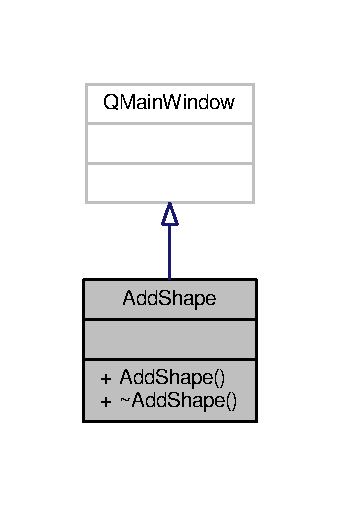
\includegraphics[width=163pt]{classAddShape__inherit__graph}
\end{center}
\end{figure}


Collaboration diagram for Add\+Shape\+:\nopagebreak
\begin{figure}[H]
\begin{center}
\leavevmode
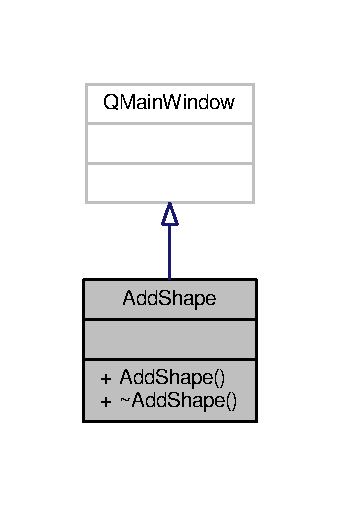
\includegraphics[width=163pt]{classAddShape__coll__graph}
\end{center}
\end{figure}
\subsection*{Signals}
\begin{DoxyCompactItemize}
\item 
void \hyperlink{classAddShape_a6f79ea980ff8d6e7001c0b9b48d5ddb4}{update\+\_\+\+Window} ()
\begin{DoxyCompactList}\small\item\em This calls an update in the window. \end{DoxyCompactList}\end{DoxyCompactItemize}
\subsection*{Public Member Functions}
\begin{DoxyCompactItemize}
\item 
\hyperlink{classAddShape_a7d99059cc9f818e4225803aa2c624723}{Add\+Shape} (Q\+Widget $\ast$parent, \hyperlink{classmyStd_1_1vector}{my\+Std\+::vector}$<$ \hyperlink{classShape}{Shape} $\ast$ $>$ \&, bool \&)
\begin{DoxyCompactList}\small\item\em Constructor for creating the pop-\/up for the \hyperlink{classAddShape}{Add\+Shape} button. \end{DoxyCompactList}\item 
\hyperlink{classAddShape_aefd175938403da086e12162e19705939}{$\sim$\+Add\+Shape} ()
\begin{DoxyCompactList}\small\item\em Destructor of \hyperlink{classAddShape}{Add\+Shape}. \end{DoxyCompactList}\end{DoxyCompactItemize}


\subsection{Detailed Description}
\hyperlink{classAddShape}{Add\+Shape} class that provides functionality for the add shape button. 

\subsection{Constructor \& Destructor Documentation}
\index{Add\+Shape@{Add\+Shape}!Add\+Shape@{Add\+Shape}}
\index{Add\+Shape@{Add\+Shape}!Add\+Shape@{Add\+Shape}}
\subsubsection[{\texorpdfstring{Add\+Shape(\+Q\+Widget $\ast$parent, my\+Std\+::vector$<$ Shape $\ast$ $>$ \&, bool \&)}{AddShape(QWidget *parent, myStd::vector< Shape * > &, bool &)}}]{\setlength{\rightskip}{0pt plus 5cm}Add\+Shape\+::\+Add\+Shape (
\begin{DoxyParamCaption}
\item[{Q\+Widget $\ast$}]{parent, }
\item[{{\bf my\+Std\+::vector}$<$ {\bf Shape} $\ast$ $>$ \&}]{shapes, }
\item[{bool \&}]{ok}
\end{DoxyParamCaption}
)\hspace{0.3cm}{\ttfamily [explicit]}}\hypertarget{classAddShape_a7d99059cc9f818e4225803aa2c624723}{}\label{classAddShape_a7d99059cc9f818e4225803aa2c624723}


Constructor for creating the pop-\/up for the \hyperlink{classAddShape}{Add\+Shape} button. 


\begin{DoxyParams}{Parameters}
{\em parent} & of the addshape window \\
\hline
\end{DoxyParams}
\index{Add\+Shape@{Add\+Shape}!````~Add\+Shape@{$\sim$\+Add\+Shape}}
\index{````~Add\+Shape@{$\sim$\+Add\+Shape}!Add\+Shape@{Add\+Shape}}
\subsubsection[{\texorpdfstring{$\sim$\+Add\+Shape()}{~AddShape()}}]{\setlength{\rightskip}{0pt plus 5cm}Add\+Shape\+::$\sim$\+Add\+Shape (
\begin{DoxyParamCaption}
{}
\end{DoxyParamCaption}
)}\hypertarget{classAddShape_aefd175938403da086e12162e19705939}{}\label{classAddShape_aefd175938403da086e12162e19705939}


Destructor of \hyperlink{classAddShape}{Add\+Shape}. 



\subsection{Member Function Documentation}
\index{Add\+Shape@{Add\+Shape}!update\+\_\+\+Window@{update\+\_\+\+Window}}
\index{update\+\_\+\+Window@{update\+\_\+\+Window}!Add\+Shape@{Add\+Shape}}
\subsubsection[{\texorpdfstring{update\+\_\+\+Window}{update_Window}}]{\setlength{\rightskip}{0pt plus 5cm}void Add\+Shape\+::update\+\_\+\+Window (
\begin{DoxyParamCaption}
{}
\end{DoxyParamCaption}
)\hspace{0.3cm}{\ttfamily [signal]}}\hypertarget{classAddShape_a6f79ea980ff8d6e7001c0b9b48d5ddb4}{}\label{classAddShape_a6f79ea980ff8d6e7001c0b9b48d5ddb4}


This calls an update in the window. 



The documentation for this class was generated from the following files\+:\begin{DoxyCompactItemize}
\item 
Group Project/\+Scrum\+Of\+The\+Earth/\hyperlink{addshape_8h}{addshape.\+h}\item 
Group Project/\+Scrum\+Of\+The\+Earth/\hyperlink{addshape_8cpp}{addshape.\+cpp}\end{DoxyCompactItemize}

\hypertarget{classCircle}{}\section{Circle Class Reference}
\label{classCircle}\index{Circle@{Circle}}


\hyperlink{classCircle}{Circle} class that Q\+Painter can draw.  




{\ttfamily \#include $<$circle.\+h$>$}



Inheritance diagram for Circle\+:\nopagebreak
\begin{figure}[H]
\begin{center}
\leavevmode
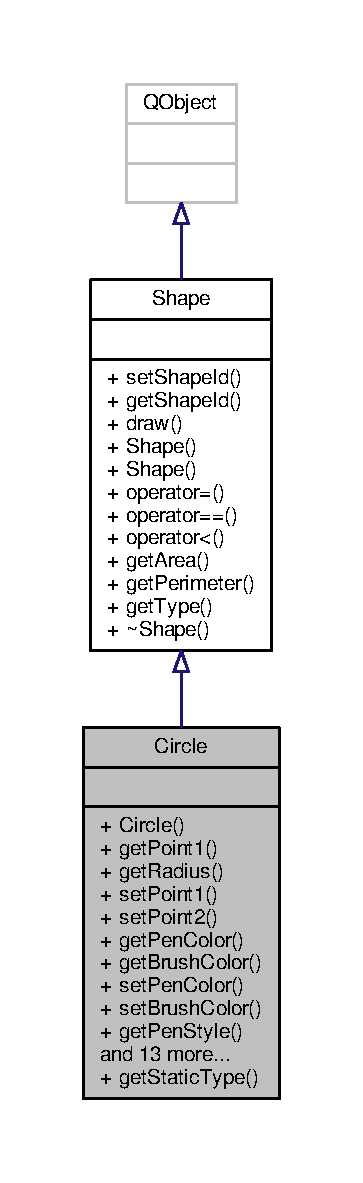
\includegraphics[height=550pt]{classCircle__inherit__graph}
\end{center}
\end{figure}


Collaboration diagram for Circle\+:\nopagebreak
\begin{figure}[H]
\begin{center}
\leavevmode
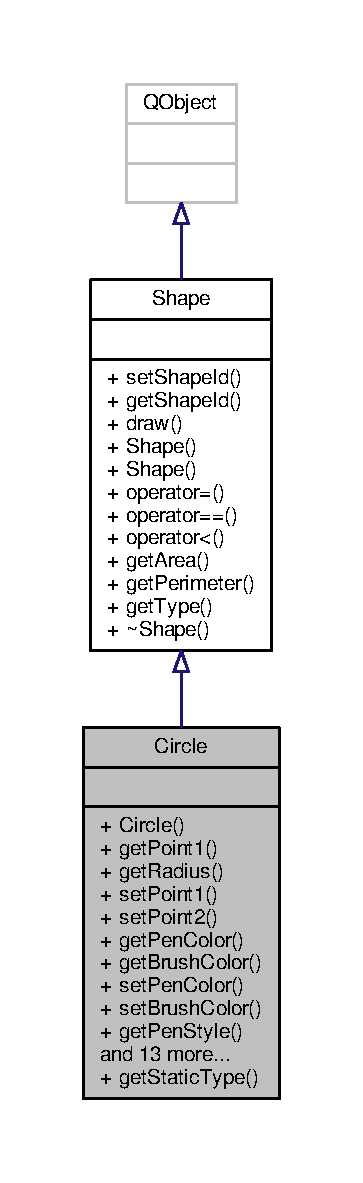
\includegraphics[height=550pt]{classCircle__coll__graph}
\end{center}
\end{figure}
\subsection*{Public Member Functions}
\begin{DoxyCompactItemize}
\item 
\hyperlink{classCircle_a40e653e2eecf4335d2125c97700dff3c}{Circle} (unsigned int i, int x, int y, int r, Qt\+::\+Global\+Color pc, Qt\+::\+Global\+Color bc, Qt\+::\+Pen\+Style ps, \hyperlink{shape__input__file__specs_8txt_a622efdcfef6789d4367974d2fe79019e}{Qt\+::\+Pen\+Cap\+Style} pcs, \hyperlink{shape__input__file__specs_8txt_a007db2043c6063881de2043c05c9c4a9}{Qt\+::\+Pen\+Join\+Style} pjs, \hyperlink{shape__input__file__specs_8txt_ad07f6fe6c28dcb0b3bdc324a72d0051f}{Qt\+::\+Brush\+Style} bs, int pw)
\begin{DoxyCompactList}\small\item\em All properties contructor. \end{DoxyCompactList}\item 
Q\+Point \hyperlink{classCircle_a363e30a4f7d06116167e77e271955998}{get\+Point1} ()
\begin{DoxyCompactList}\small\item\em Gets the center of the circle as a point. \end{DoxyCompactList}\item 
int \hyperlink{classCircle_adfc2e5e026f5d80215563cc42260a237}{get\+Radius} ()
\begin{DoxyCompactList}\small\item\em Gets the radius of the circle. \end{DoxyCompactList}\item 
void \hyperlink{classCircle_a60e5c24fe969240435725aa608bed3dd}{set\+Point1} (Q\+Point p1)
\begin{DoxyCompactList}\small\item\em Sets the center of the circle to the given point. \end{DoxyCompactList}\item 
void \hyperlink{classCircle_ad1c743962a2fc94b46cc80fbf88705ed}{set\+Point2} (int r)
\begin{DoxyCompactList}\small\item\em Sets the radius. \end{DoxyCompactList}\item 
Qt\+::\+Global\+Color \hyperlink{classCircle_a56a594eac870bedf7c268a024bbd92d3}{get\+Pen\+Color} ()
\begin{DoxyCompactList}\small\item\em Gets the pen color stored in this shape. \end{DoxyCompactList}\item 
Qt\+::\+Global\+Color \hyperlink{classCircle_a82bde4b53ba1026e640db30b1096d60b}{get\+Brush\+Color} ()
\begin{DoxyCompactList}\small\item\em Gets the Brush color stored in the \hyperlink{classShape}{Shape}. \end{DoxyCompactList}\item 
void \hyperlink{classCircle_ad7ea24061f3ac147c396ca258b132018}{set\+Pen\+Color} (Qt\+::\+Global\+Color pc)
\begin{DoxyCompactList}\small\item\em Sets the color of the pen to the given color. \end{DoxyCompactList}\item 
void \hyperlink{classCircle_adc5d39dd16a7f02a4142903d17b02744}{set\+Brush\+Color} (Qt\+::\+Global\+Color bc)
\begin{DoxyCompactList}\small\item\em Sets the color of the Brush to the given color. \end{DoxyCompactList}\item 
Qt\+::\+Pen\+Style \hyperlink{classCircle_aca52e370c08797fd90af17499bc33e5b}{get\+Pen\+Style} ()
\begin{DoxyCompactList}\small\item\em Gets the style of the pen stored in the shape. \end{DoxyCompactList}\item 
void \hyperlink{classCircle_a0eb4403f9655b48e774e2be89dd18088}{set\+Pen\+Style} (Qt\+::\+Pen\+Style ps)
\begin{DoxyCompactList}\small\item\em Sets the style of the pen to the given style. \end{DoxyCompactList}\item 
\hyperlink{shape__input__file__specs_8txt_a622efdcfef6789d4367974d2fe79019e}{Qt\+::\+Pen\+Cap\+Style} \hyperlink{classCircle_abaf3d67a11b83ba5df3ce7a8a382bbc1}{get\+Pen\+Cap\+Style} ()
\begin{DoxyCompactList}\small\item\em Gets the pen cap style that is stored in this \hyperlink{classShape}{Shape}. \end{DoxyCompactList}\item 
void \hyperlink{classCircle_ad93fa94177ed8bfbb9c695b6bab9d8b3}{set\+Pen\+Cap\+Style} (\hyperlink{shape__input__file__specs_8txt_a622efdcfef6789d4367974d2fe79019e}{Qt\+::\+Pen\+Cap\+Style} pcs)
\begin{DoxyCompactList}\small\item\em Sets the Pen Cap Style to the given Pen Cap Style. \end{DoxyCompactList}\item 
\hyperlink{shape__input__file__specs_8txt_a007db2043c6063881de2043c05c9c4a9}{Qt\+::\+Pen\+Join\+Style} \hyperlink{classCircle_ac4ecd23537522a25d55e9d7197c7d9b5}{get\+Pen\+Join\+Style} ()
\begin{DoxyCompactList}\small\item\em Gets the Pen Join Style. \end{DoxyCompactList}\item 
void \hyperlink{classCircle_a1b0c03d17c9fc49bbcb6e8708f9bd827}{set\+Pen\+Join\+Style} (\hyperlink{shape__input__file__specs_8txt_a007db2043c6063881de2043c05c9c4a9}{Qt\+::\+Pen\+Join\+Style} pjs)
\begin{DoxyCompactList}\small\item\em Sets the pen join style to the given style. \end{DoxyCompactList}\item 
\hyperlink{shape__input__file__specs_8txt_ad07f6fe6c28dcb0b3bdc324a72d0051f}{Qt\+::\+Brush\+Style} \hyperlink{classCircle_a4ec3092959992a2a6b2782e622617bda}{get\+Brush\+Style} ()
\begin{DoxyCompactList}\small\item\em Gets the Brush Style. \end{DoxyCompactList}\item 
void \hyperlink{classCircle_a8029072b1eea3ef62c9010f68257b112}{set\+Brush\+Style} (\hyperlink{shape__input__file__specs_8txt_ad07f6fe6c28dcb0b3bdc324a72d0051f}{Qt\+::\+Brush\+Style} bs)
\begin{DoxyCompactList}\small\item\em Sets the Brush Style to the given Brush Style. \end{DoxyCompactList}\item 
int \hyperlink{classCircle_ab7d1e660ddced5d2f6fd36290f06083a}{get\+Pen\+Width} ()
\begin{DoxyCompactList}\small\item\em Gets the width of the pen. \end{DoxyCompactList}\item 
void \hyperlink{classCircle_abe124577ed86f9d9bcf77b0a5fdaca73}{set\+Pen\+Width} (int pw)
\begin{DoxyCompactList}\small\item\em Sets the width of the pen to the given width. \end{DoxyCompactList}\item 
virtual void \hyperlink{classCircle_aebc2ff1cc810905bc557d54e76aef936}{draw} (Q\+Painter \&paint, bool)
\begin{DoxyCompactList}\small\item\em Virtual function to draw shapes. \end{DoxyCompactList}\item 
virtual int \hyperlink{classCircle_ac13b29eb5095b4fd8e6c25ba50dd9131}{get\+Type} ()
\begin{DoxyCompactList}\small\item\em Gets the type of the shape. \end{DoxyCompactList}\item 
virtual double \hyperlink{classCircle_ae770cbdb3a0148a9db411fb3b0f87b9a}{get\+Area} ()
\begin{DoxyCompactList}\small\item\em Gets the area of the given shape. \end{DoxyCompactList}\item 
virtual double \hyperlink{classCircle_af9a14f66b467788f8395ea587357a93f}{get\+Perimeter} ()
\begin{DoxyCompactList}\small\item\em Gets the perimeter of the given shape. \end{DoxyCompactList}\end{DoxyCompactItemize}
\subsection*{Static Public Member Functions}
\begin{DoxyCompactItemize}
\item 
static int \hyperlink{classCircle_ac5e287c2511f325888d340b6555d51b5}{get\+Static\+Type} ()
\begin{DoxyCompactList}\small\item\em Gets the type of object. \end{DoxyCompactList}\end{DoxyCompactItemize}


\subsection{Detailed Description}
\hyperlink{classCircle}{Circle} class that Q\+Painter can draw. 

\subsection{Constructor \& Destructor Documentation}
\index{Circle@{Circle}!Circle@{Circle}}
\index{Circle@{Circle}!Circle@{Circle}}
\subsubsection[{\texorpdfstring{Circle(unsigned int i, int x, int y, int r, Qt\+::\+Global\+Color pc, Qt\+::\+Global\+Color bc, Qt\+::\+Pen\+Style ps, Qt\+::\+Pen\+Cap\+Style pcs, Qt\+::\+Pen\+Join\+Style pjs, Qt\+::\+Brush\+Style bs, int pw)}{Circle(unsigned int i, int x, int y, int r, Qt::GlobalColor pc, Qt::GlobalColor bc, Qt::PenStyle ps, Qt::PenCapStyle pcs, Qt::PenJoinStyle pjs, Qt::BrushStyle bs, int pw)}}]{\setlength{\rightskip}{0pt plus 5cm}Circle\+::\+Circle (
\begin{DoxyParamCaption}
\item[{unsigned int}]{i, }
\item[{int}]{x, }
\item[{int}]{y, }
\item[{int}]{r, }
\item[{Qt\+::\+Global\+Color}]{pc, }
\item[{Qt\+::\+Global\+Color}]{bc, }
\item[{Qt\+::\+Pen\+Style}]{ps, }
\item[{{\bf Qt\+::\+Pen\+Cap\+Style}}]{pcs, }
\item[{{\bf Qt\+::\+Pen\+Join\+Style}}]{pjs, }
\item[{{\bf Qt\+::\+Brush\+Style}}]{bs, }
\item[{int}]{pw}
\end{DoxyParamCaption}
)}\hypertarget{classCircle_a40e653e2eecf4335d2125c97700dff3c}{}\label{classCircle_a40e653e2eecf4335d2125c97700dff3c}


All properties contructor. 


\begin{DoxyParams}{Parameters}
{\em id} & \\
\hline
{\em x} & coordinate \\
\hline
{\em y} & coordinate \\
\hline
{\em radius} & \\
\hline
{\em pen\+Color} & \\
\hline
{\em brush\+Color} & \\
\hline
{\em pen\+Style} & \\
\hline
{\em pen\+Cap\+Style} & \\
\hline
{\em pen\+Join\+Style} & \\
\hline
{\em brush\+Style} & \\
\hline
{\em pen\+Width} & \\
\hline
\end{DoxyParams}


\subsection{Member Function Documentation}
\index{Circle@{Circle}!draw@{draw}}
\index{draw@{draw}!Circle@{Circle}}
\subsubsection[{\texorpdfstring{draw(\+Q\+Painter \&paint, bool)}{draw(QPainter &paint, bool)}}]{\setlength{\rightskip}{0pt plus 5cm}void Circle\+::draw (
\begin{DoxyParamCaption}
\item[{Q\+Painter \&}]{, }
\item[{bool}]{}
\end{DoxyParamCaption}
)\hspace{0.3cm}{\ttfamily [virtual]}}\hypertarget{classCircle_aebc2ff1cc810905bc557d54e76aef936}{}\label{classCircle_aebc2ff1cc810905bc557d54e76aef936}


Virtual function to draw shapes. 



Implements \hyperlink{classShape_a47dae32819e64fb32f3357f31978293f}{Shape}.

\index{Circle@{Circle}!get\+Area@{get\+Area}}
\index{get\+Area@{get\+Area}!Circle@{Circle}}
\subsubsection[{\texorpdfstring{get\+Area()}{getArea()}}]{\setlength{\rightskip}{0pt plus 5cm}virtual double Circle\+::get\+Area (
\begin{DoxyParamCaption}
{}
\end{DoxyParamCaption}
)\hspace{0.3cm}{\ttfamily [inline]}, {\ttfamily [virtual]}}\hypertarget{classCircle_ae770cbdb3a0148a9db411fb3b0f87b9a}{}\label{classCircle_ae770cbdb3a0148a9db411fb3b0f87b9a}


Gets the area of the given shape. 

\begin{DoxyReturn}{Returns}
Area as a double 
\end{DoxyReturn}


Reimplemented from \hyperlink{classShape_ac29f8bce0d038c84470028c6819a79ab}{Shape}.

\index{Circle@{Circle}!get\+Brush\+Color@{get\+Brush\+Color}}
\index{get\+Brush\+Color@{get\+Brush\+Color}!Circle@{Circle}}
\subsubsection[{\texorpdfstring{get\+Brush\+Color()}{getBrushColor()}}]{\setlength{\rightskip}{0pt plus 5cm}Qt\+::\+Global\+Color Circle\+::get\+Brush\+Color (
\begin{DoxyParamCaption}
{}
\end{DoxyParamCaption}
)\hspace{0.3cm}{\ttfamily [inline]}}\hypertarget{classCircle_a82bde4b53ba1026e640db30b1096d60b}{}\label{classCircle_a82bde4b53ba1026e640db30b1096d60b}


Gets the Brush color stored in the \hyperlink{classShape}{Shape}. 

\begin{DoxyReturn}{Returns}
Color of the Brush 
\end{DoxyReturn}
\index{Circle@{Circle}!get\+Brush\+Style@{get\+Brush\+Style}}
\index{get\+Brush\+Style@{get\+Brush\+Style}!Circle@{Circle}}
\subsubsection[{\texorpdfstring{get\+Brush\+Style()}{getBrushStyle()}}]{\setlength{\rightskip}{0pt plus 5cm}{\bf Qt\+::\+Brush\+Style} Circle\+::get\+Brush\+Style (
\begin{DoxyParamCaption}
{}
\end{DoxyParamCaption}
)\hspace{0.3cm}{\ttfamily [inline]}}\hypertarget{classCircle_a4ec3092959992a2a6b2782e622617bda}{}\label{classCircle_a4ec3092959992a2a6b2782e622617bda}


Gets the Brush Style. 

\begin{DoxyReturn}{Returns}
Brush\+Style 
\end{DoxyReturn}
\index{Circle@{Circle}!get\+Pen\+Cap\+Style@{get\+Pen\+Cap\+Style}}
\index{get\+Pen\+Cap\+Style@{get\+Pen\+Cap\+Style}!Circle@{Circle}}
\subsubsection[{\texorpdfstring{get\+Pen\+Cap\+Style()}{getPenCapStyle()}}]{\setlength{\rightskip}{0pt plus 5cm}{\bf Qt\+::\+Pen\+Cap\+Style} Circle\+::get\+Pen\+Cap\+Style (
\begin{DoxyParamCaption}
{}
\end{DoxyParamCaption}
)\hspace{0.3cm}{\ttfamily [inline]}}\hypertarget{classCircle_abaf3d67a11b83ba5df3ce7a8a382bbc1}{}\label{classCircle_abaf3d67a11b83ba5df3ce7a8a382bbc1}


Gets the pen cap style that is stored in this \hyperlink{classShape}{Shape}. 

\begin{DoxyReturn}{Returns}
Pen\+Cap\+Style 
\end{DoxyReturn}
\index{Circle@{Circle}!get\+Pen\+Color@{get\+Pen\+Color}}
\index{get\+Pen\+Color@{get\+Pen\+Color}!Circle@{Circle}}
\subsubsection[{\texorpdfstring{get\+Pen\+Color()}{getPenColor()}}]{\setlength{\rightskip}{0pt plus 5cm}Qt\+::\+Global\+Color Circle\+::get\+Pen\+Color (
\begin{DoxyParamCaption}
{}
\end{DoxyParamCaption}
)\hspace{0.3cm}{\ttfamily [inline]}}\hypertarget{classCircle_a56a594eac870bedf7c268a024bbd92d3}{}\label{classCircle_a56a594eac870bedf7c268a024bbd92d3}


Gets the pen color stored in this shape. 

\begin{DoxyReturn}{Returns}
Color of the pen 
\end{DoxyReturn}
\index{Circle@{Circle}!get\+Pen\+Join\+Style@{get\+Pen\+Join\+Style}}
\index{get\+Pen\+Join\+Style@{get\+Pen\+Join\+Style}!Circle@{Circle}}
\subsubsection[{\texorpdfstring{get\+Pen\+Join\+Style()}{getPenJoinStyle()}}]{\setlength{\rightskip}{0pt plus 5cm}{\bf Qt\+::\+Pen\+Join\+Style} Circle\+::get\+Pen\+Join\+Style (
\begin{DoxyParamCaption}
{}
\end{DoxyParamCaption}
)\hspace{0.3cm}{\ttfamily [inline]}}\hypertarget{classCircle_ac4ecd23537522a25d55e9d7197c7d9b5}{}\label{classCircle_ac4ecd23537522a25d55e9d7197c7d9b5}


Gets the Pen Join Style. 

\begin{DoxyReturn}{Returns}
Pen\+Join\+Style 
\end{DoxyReturn}
\index{Circle@{Circle}!get\+Pen\+Style@{get\+Pen\+Style}}
\index{get\+Pen\+Style@{get\+Pen\+Style}!Circle@{Circle}}
\subsubsection[{\texorpdfstring{get\+Pen\+Style()}{getPenStyle()}}]{\setlength{\rightskip}{0pt plus 5cm}Qt\+::\+Pen\+Style Circle\+::get\+Pen\+Style (
\begin{DoxyParamCaption}
{}
\end{DoxyParamCaption}
)\hspace{0.3cm}{\ttfamily [inline]}}\hypertarget{classCircle_aca52e370c08797fd90af17499bc33e5b}{}\label{classCircle_aca52e370c08797fd90af17499bc33e5b}


Gets the style of the pen stored in the shape. 

\begin{DoxyReturn}{Returns}
Style of the pen 
\end{DoxyReturn}
\index{Circle@{Circle}!get\+Pen\+Width@{get\+Pen\+Width}}
\index{get\+Pen\+Width@{get\+Pen\+Width}!Circle@{Circle}}
\subsubsection[{\texorpdfstring{get\+Pen\+Width()}{getPenWidth()}}]{\setlength{\rightskip}{0pt plus 5cm}int Circle\+::get\+Pen\+Width (
\begin{DoxyParamCaption}
{}
\end{DoxyParamCaption}
)\hspace{0.3cm}{\ttfamily [inline]}}\hypertarget{classCircle_ab7d1e660ddced5d2f6fd36290f06083a}{}\label{classCircle_ab7d1e660ddced5d2f6fd36290f06083a}


Gets the width of the pen. 

\begin{DoxyReturn}{Returns}
pen\+Width 
\end{DoxyReturn}
\index{Circle@{Circle}!get\+Perimeter@{get\+Perimeter}}
\index{get\+Perimeter@{get\+Perimeter}!Circle@{Circle}}
\subsubsection[{\texorpdfstring{get\+Perimeter()}{getPerimeter()}}]{\setlength{\rightskip}{0pt plus 5cm}virtual double Circle\+::get\+Perimeter (
\begin{DoxyParamCaption}
{}
\end{DoxyParamCaption}
)\hspace{0.3cm}{\ttfamily [inline]}, {\ttfamily [virtual]}}\hypertarget{classCircle_af9a14f66b467788f8395ea587357a93f}{}\label{classCircle_af9a14f66b467788f8395ea587357a93f}


Gets the perimeter of the given shape. 

\begin{DoxyReturn}{Returns}
Perimeter as a double 
\end{DoxyReturn}


Reimplemented from \hyperlink{classShape_a391744b6bce96df044139dcbd1ae0aa8}{Shape}.

\index{Circle@{Circle}!get\+Point1@{get\+Point1}}
\index{get\+Point1@{get\+Point1}!Circle@{Circle}}
\subsubsection[{\texorpdfstring{get\+Point1()}{getPoint1()}}]{\setlength{\rightskip}{0pt plus 5cm}Q\+Point Circle\+::get\+Point1 (
\begin{DoxyParamCaption}
{}
\end{DoxyParamCaption}
)\hspace{0.3cm}{\ttfamily [inline]}}\hypertarget{classCircle_a363e30a4f7d06116167e77e271955998}{}\label{classCircle_a363e30a4f7d06116167e77e271955998}


Gets the center of the circle as a point. 

\begin{DoxyReturn}{Returns}
Center of circle as Q\+Point 
\end{DoxyReturn}
\index{Circle@{Circle}!get\+Radius@{get\+Radius}}
\index{get\+Radius@{get\+Radius}!Circle@{Circle}}
\subsubsection[{\texorpdfstring{get\+Radius()}{getRadius()}}]{\setlength{\rightskip}{0pt plus 5cm}int Circle\+::get\+Radius (
\begin{DoxyParamCaption}
{}
\end{DoxyParamCaption}
)\hspace{0.3cm}{\ttfamily [inline]}}\hypertarget{classCircle_adfc2e5e026f5d80215563cc42260a237}{}\label{classCircle_adfc2e5e026f5d80215563cc42260a237}


Gets the radius of the circle. 

\begin{DoxyReturn}{Returns}
radius 
\end{DoxyReturn}
\index{Circle@{Circle}!get\+Static\+Type@{get\+Static\+Type}}
\index{get\+Static\+Type@{get\+Static\+Type}!Circle@{Circle}}
\subsubsection[{\texorpdfstring{get\+Static\+Type()}{getStaticType()}}]{\setlength{\rightskip}{0pt plus 5cm}static int Circle\+::get\+Static\+Type (
\begin{DoxyParamCaption}
{}
\end{DoxyParamCaption}
)\hspace{0.3cm}{\ttfamily [inline]}, {\ttfamily [static]}}\hypertarget{classCircle_ac5e287c2511f325888d340b6555d51b5}{}\label{classCircle_ac5e287c2511f325888d340b6555d51b5}


Gets the type of object. 

\begin{DoxyReturn}{Returns}
Type as int 
\end{DoxyReturn}
\index{Circle@{Circle}!get\+Type@{get\+Type}}
\index{get\+Type@{get\+Type}!Circle@{Circle}}
\subsubsection[{\texorpdfstring{get\+Type()}{getType()}}]{\setlength{\rightskip}{0pt plus 5cm}virtual int Circle\+::get\+Type (
\begin{DoxyParamCaption}
{}
\end{DoxyParamCaption}
)\hspace{0.3cm}{\ttfamily [inline]}, {\ttfamily [virtual]}}\hypertarget{classCircle_ac13b29eb5095b4fd8e6c25ba50dd9131}{}\label{classCircle_ac13b29eb5095b4fd8e6c25ba50dd9131}


Gets the type of the shape. 

\begin{DoxyReturn}{Returns}
type as an int 
\end{DoxyReturn}


Implements \hyperlink{classShape_a3d15adf2a1d746928f9be98105096eda}{Shape}.

\index{Circle@{Circle}!set\+Brush\+Color@{set\+Brush\+Color}}
\index{set\+Brush\+Color@{set\+Brush\+Color}!Circle@{Circle}}
\subsubsection[{\texorpdfstring{set\+Brush\+Color(\+Qt\+::\+Global\+Color bc)}{setBrushColor(Qt::GlobalColor bc)}}]{\setlength{\rightskip}{0pt plus 5cm}void Circle\+::set\+Brush\+Color (
\begin{DoxyParamCaption}
\item[{Qt\+::\+Global\+Color}]{bc}
\end{DoxyParamCaption}
)\hspace{0.3cm}{\ttfamily [inline]}}\hypertarget{classCircle_adc5d39dd16a7f02a4142903d17b02744}{}\label{classCircle_adc5d39dd16a7f02a4142903d17b02744}


Sets the color of the Brush to the given color. 


\begin{DoxyParams}{Parameters}
{\em brush\+Color} & \\
\hline
\end{DoxyParams}
\index{Circle@{Circle}!set\+Brush\+Style@{set\+Brush\+Style}}
\index{set\+Brush\+Style@{set\+Brush\+Style}!Circle@{Circle}}
\subsubsection[{\texorpdfstring{set\+Brush\+Style(\+Qt\+::\+Brush\+Style bs)}{setBrushStyle(Qt::BrushStyle bs)}}]{\setlength{\rightskip}{0pt plus 5cm}void Circle\+::set\+Brush\+Style (
\begin{DoxyParamCaption}
\item[{{\bf Qt\+::\+Brush\+Style}}]{bs}
\end{DoxyParamCaption}
)\hspace{0.3cm}{\ttfamily [inline]}}\hypertarget{classCircle_a8029072b1eea3ef62c9010f68257b112}{}\label{classCircle_a8029072b1eea3ef62c9010f68257b112}


Sets the Brush Style to the given Brush Style. 


\begin{DoxyParams}{Parameters}
{\em brush\+Style} & \\
\hline
\end{DoxyParams}
\index{Circle@{Circle}!set\+Pen\+Cap\+Style@{set\+Pen\+Cap\+Style}}
\index{set\+Pen\+Cap\+Style@{set\+Pen\+Cap\+Style}!Circle@{Circle}}
\subsubsection[{\texorpdfstring{set\+Pen\+Cap\+Style(\+Qt\+::\+Pen\+Cap\+Style pcs)}{setPenCapStyle(Qt::PenCapStyle pcs)}}]{\setlength{\rightskip}{0pt plus 5cm}void Circle\+::set\+Pen\+Cap\+Style (
\begin{DoxyParamCaption}
\item[{{\bf Qt\+::\+Pen\+Cap\+Style}}]{pcs}
\end{DoxyParamCaption}
)\hspace{0.3cm}{\ttfamily [inline]}}\hypertarget{classCircle_ad93fa94177ed8bfbb9c695b6bab9d8b3}{}\label{classCircle_ad93fa94177ed8bfbb9c695b6bab9d8b3}


Sets the Pen Cap Style to the given Pen Cap Style. 


\begin{DoxyParams}{Parameters}
{\em pen\+Cap\+Style} & \\
\hline
\end{DoxyParams}
\index{Circle@{Circle}!set\+Pen\+Color@{set\+Pen\+Color}}
\index{set\+Pen\+Color@{set\+Pen\+Color}!Circle@{Circle}}
\subsubsection[{\texorpdfstring{set\+Pen\+Color(\+Qt\+::\+Global\+Color pc)}{setPenColor(Qt::GlobalColor pc)}}]{\setlength{\rightskip}{0pt plus 5cm}void Circle\+::set\+Pen\+Color (
\begin{DoxyParamCaption}
\item[{Qt\+::\+Global\+Color}]{pc}
\end{DoxyParamCaption}
)\hspace{0.3cm}{\ttfamily [inline]}}\hypertarget{classCircle_ad7ea24061f3ac147c396ca258b132018}{}\label{classCircle_ad7ea24061f3ac147c396ca258b132018}


Sets the color of the pen to the given color. 


\begin{DoxyParams}{Parameters}
{\em pen\+Color} & \\
\hline
\end{DoxyParams}
\index{Circle@{Circle}!set\+Pen\+Join\+Style@{set\+Pen\+Join\+Style}}
\index{set\+Pen\+Join\+Style@{set\+Pen\+Join\+Style}!Circle@{Circle}}
\subsubsection[{\texorpdfstring{set\+Pen\+Join\+Style(\+Qt\+::\+Pen\+Join\+Style pjs)}{setPenJoinStyle(Qt::PenJoinStyle pjs)}}]{\setlength{\rightskip}{0pt plus 5cm}void Circle\+::set\+Pen\+Join\+Style (
\begin{DoxyParamCaption}
\item[{{\bf Qt\+::\+Pen\+Join\+Style}}]{pjs}
\end{DoxyParamCaption}
)\hspace{0.3cm}{\ttfamily [inline]}}\hypertarget{classCircle_a1b0c03d17c9fc49bbcb6e8708f9bd827}{}\label{classCircle_a1b0c03d17c9fc49bbcb6e8708f9bd827}


Sets the pen join style to the given style. 


\begin{DoxyParams}{Parameters}
{\em pen\+Join\+Style} & \\
\hline
\end{DoxyParams}
\index{Circle@{Circle}!set\+Pen\+Style@{set\+Pen\+Style}}
\index{set\+Pen\+Style@{set\+Pen\+Style}!Circle@{Circle}}
\subsubsection[{\texorpdfstring{set\+Pen\+Style(\+Qt\+::\+Pen\+Style ps)}{setPenStyle(Qt::PenStyle ps)}}]{\setlength{\rightskip}{0pt plus 5cm}void Circle\+::set\+Pen\+Style (
\begin{DoxyParamCaption}
\item[{Qt\+::\+Pen\+Style}]{ps}
\end{DoxyParamCaption}
)\hspace{0.3cm}{\ttfamily [inline]}}\hypertarget{classCircle_a0eb4403f9655b48e774e2be89dd18088}{}\label{classCircle_a0eb4403f9655b48e774e2be89dd18088}


Sets the style of the pen to the given style. 


\begin{DoxyParams}{Parameters}
{\em pen\+Style} & \\
\hline
\end{DoxyParams}
\index{Circle@{Circle}!set\+Pen\+Width@{set\+Pen\+Width}}
\index{set\+Pen\+Width@{set\+Pen\+Width}!Circle@{Circle}}
\subsubsection[{\texorpdfstring{set\+Pen\+Width(int pw)}{setPenWidth(int pw)}}]{\setlength{\rightskip}{0pt plus 5cm}void Circle\+::set\+Pen\+Width (
\begin{DoxyParamCaption}
\item[{int}]{pw}
\end{DoxyParamCaption}
)\hspace{0.3cm}{\ttfamily [inline]}}\hypertarget{classCircle_abe124577ed86f9d9bcf77b0a5fdaca73}{}\label{classCircle_abe124577ed86f9d9bcf77b0a5fdaca73}


Sets the width of the pen to the given width. 


\begin{DoxyParams}{Parameters}
{\em pen\+Width} & \\
\hline
\end{DoxyParams}
\index{Circle@{Circle}!set\+Point1@{set\+Point1}}
\index{set\+Point1@{set\+Point1}!Circle@{Circle}}
\subsubsection[{\texorpdfstring{set\+Point1(\+Q\+Point p1)}{setPoint1(QPoint p1)}}]{\setlength{\rightskip}{0pt plus 5cm}void Circle\+::set\+Point1 (
\begin{DoxyParamCaption}
\item[{Q\+Point}]{p1}
\end{DoxyParamCaption}
)\hspace{0.3cm}{\ttfamily [inline]}}\hypertarget{classCircle_a60e5c24fe969240435725aa608bed3dd}{}\label{classCircle_a60e5c24fe969240435725aa608bed3dd}


Sets the center of the circle to the given point. 


\begin{DoxyParams}{Parameters}
{\em Center} & Point \\
\hline
\end{DoxyParams}
\index{Circle@{Circle}!set\+Point2@{set\+Point2}}
\index{set\+Point2@{set\+Point2}!Circle@{Circle}}
\subsubsection[{\texorpdfstring{set\+Point2(int r)}{setPoint2(int r)}}]{\setlength{\rightskip}{0pt plus 5cm}void Circle\+::set\+Point2 (
\begin{DoxyParamCaption}
\item[{int}]{r}
\end{DoxyParamCaption}
)\hspace{0.3cm}{\ttfamily [inline]}}\hypertarget{classCircle_ad1c743962a2fc94b46cc80fbf88705ed}{}\label{classCircle_ad1c743962a2fc94b46cc80fbf88705ed}


Sets the radius. 


\begin{DoxyParams}{Parameters}
{\em radius} & \\
\hline
\end{DoxyParams}


The documentation for this class was generated from the following files\+:\begin{DoxyCompactItemize}
\item 
Group Project/\+Scrum\+Of\+The\+Earth/\hyperlink{circle_8h}{circle.\+h}\item 
Group Project/\+Scrum\+Of\+The\+Earth/\hyperlink{circle_8cpp}{circle.\+cpp}\end{DoxyCompactItemize}

\hypertarget{classContactUs}{}\section{Contact\+Us Class Reference}
\label{classContactUs}\index{Contact\+Us@{Contact\+Us}}


The \hyperlink{classContactUs}{Contact\+Us} class provides functionality for the contact us window.  




{\ttfamily \#include $<$contactus.\+h$>$}



Inheritance diagram for Contact\+Us\+:\nopagebreak
\begin{figure}[H]
\begin{center}
\leavevmode
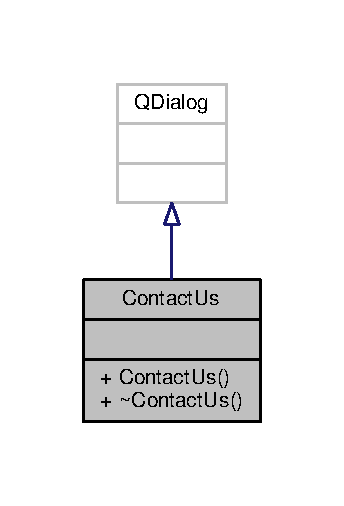
\includegraphics[width=165pt]{classContactUs__inherit__graph}
\end{center}
\end{figure}


Collaboration diagram for Contact\+Us\+:\nopagebreak
\begin{figure}[H]
\begin{center}
\leavevmode
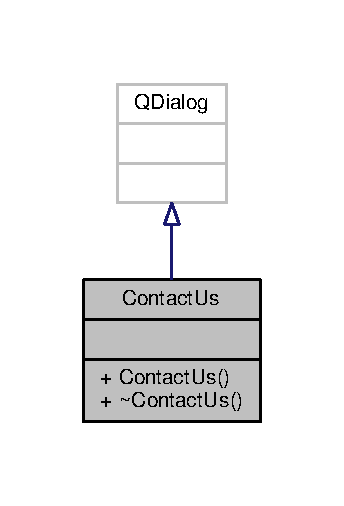
\includegraphics[width=165pt]{classContactUs__coll__graph}
\end{center}
\end{figure}
\subsection*{Public Member Functions}
\begin{DoxyCompactItemize}
\item 
\hyperlink{classContactUs_a6e20fc1c353d994a2f0bf13df4580232}{Contact\+Us} (Q\+Widget $\ast$parent=nullptr)
\begin{DoxyCompactList}\small\item\em \hyperlink{classContactUs}{Contact\+Us} constructor creates a window for the contact us information. \end{DoxyCompactList}\item 
\hyperlink{classContactUs_a44bd80bbb4908c913bb07019a609c5ba}{$\sim$\+Contact\+Us} ()
\begin{DoxyCompactList}\small\item\em Destructor for \hyperlink{classContactUs}{Contact\+Us}. \end{DoxyCompactList}\end{DoxyCompactItemize}


\subsection{Detailed Description}
The \hyperlink{classContactUs}{Contact\+Us} class provides functionality for the contact us window. 

\subsection{Constructor \& Destructor Documentation}
\index{Contact\+Us@{Contact\+Us}!Contact\+Us@{Contact\+Us}}
\index{Contact\+Us@{Contact\+Us}!Contact\+Us@{Contact\+Us}}
\subsubsection[{\texorpdfstring{Contact\+Us(\+Q\+Widget $\ast$parent=nullptr)}{ContactUs(QWidget *parent=nullptr)}}]{\setlength{\rightskip}{0pt plus 5cm}Contact\+Us\+::\+Contact\+Us (
\begin{DoxyParamCaption}
\item[{Q\+Widget $\ast$}]{parent = {\ttfamily nullptr}}
\end{DoxyParamCaption}
)\hspace{0.3cm}{\ttfamily [explicit]}}\hypertarget{classContactUs_a6e20fc1c353d994a2f0bf13df4580232}{}\label{classContactUs_a6e20fc1c353d994a2f0bf13df4580232}


\hyperlink{classContactUs}{Contact\+Us} constructor creates a window for the contact us information. 


\begin{DoxyParams}{Parameters}
{\em parent} & window \\
\hline
\end{DoxyParams}
\index{Contact\+Us@{Contact\+Us}!````~Contact\+Us@{$\sim$\+Contact\+Us}}
\index{````~Contact\+Us@{$\sim$\+Contact\+Us}!Contact\+Us@{Contact\+Us}}
\subsubsection[{\texorpdfstring{$\sim$\+Contact\+Us()}{~ContactUs()}}]{\setlength{\rightskip}{0pt plus 5cm}Contact\+Us\+::$\sim$\+Contact\+Us (
\begin{DoxyParamCaption}
{}
\end{DoxyParamCaption}
)}\hypertarget{classContactUs_a44bd80bbb4908c913bb07019a609c5ba}{}\label{classContactUs_a44bd80bbb4908c913bb07019a609c5ba}


Destructor for \hyperlink{classContactUs}{Contact\+Us}. 



The documentation for this class was generated from the following files\+:\begin{DoxyCompactItemize}
\item 
Group Project/\+Scrum\+Of\+The\+Earth/\hyperlink{contactus_8h}{contactus.\+h}\item 
Group Project/\+Scrum\+Of\+The\+Earth/\hyperlink{contactus_8cpp}{contactus.\+cpp}\end{DoxyCompactItemize}

\hypertarget{classEllipse}{}\section{Ellipse Class Reference}
\label{classEllipse}\index{Ellipse@{Ellipse}}


\hyperlink{classEllipse}{Ellipse} class that Q\+Painter can draw.  




{\ttfamily \#include $<$ellipse.\+h$>$}



Inheritance diagram for Ellipse\+:\nopagebreak
\begin{figure}[H]
\begin{center}
\leavevmode
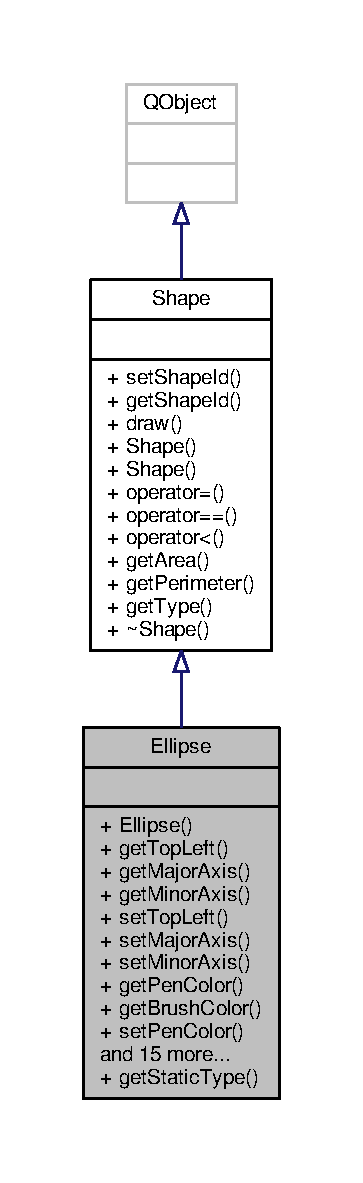
\includegraphics[height=550pt]{classEllipse__inherit__graph}
\end{center}
\end{figure}


Collaboration diagram for Ellipse\+:\nopagebreak
\begin{figure}[H]
\begin{center}
\leavevmode
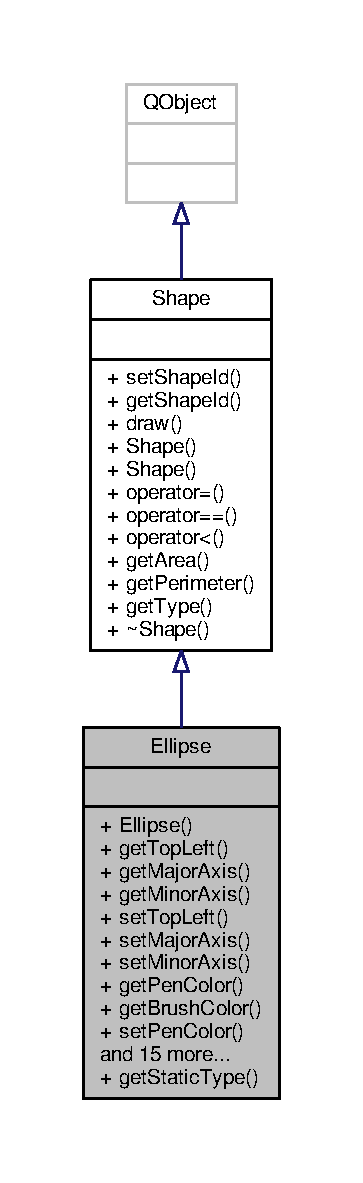
\includegraphics[height=550pt]{classEllipse__coll__graph}
\end{center}
\end{figure}
\subsection*{Public Member Functions}
\begin{DoxyCompactItemize}
\item 
\hyperlink{classEllipse_a76a451f8817fbfb5cd750621e3548cf7}{Ellipse} (unsigned int, int, int, int, int, Qt\+::\+Global\+Color, Qt\+::\+Global\+Color, Qt\+::\+Pen\+Style, \hyperlink{shape__input__file__specs_8txt_a622efdcfef6789d4367974d2fe79019e}{Qt\+::\+Pen\+Cap\+Style}, \hyperlink{shape__input__file__specs_8txt_a007db2043c6063881de2043c05c9c4a9}{Qt\+::\+Pen\+Join\+Style}, \hyperlink{shape__input__file__specs_8txt_ad07f6fe6c28dcb0b3bdc324a72d0051f}{Qt\+::\+Brush\+Style}, int)
\begin{DoxyCompactList}\small\item\em All element contructor. \end{DoxyCompactList}\item 
Q\+Point \hyperlink{classEllipse_a8d67061c0516c89e5bbcd17e1b2b22c9}{get\+Top\+Left} ()
\begin{DoxyCompactList}\small\item\em Gets the point to the top left corner. \end{DoxyCompactList}\item 
int \hyperlink{classEllipse_a4cb6a9a3ef286098d0ab36f8fecb2091}{get\+Major\+Axis} ()
\begin{DoxyCompactList}\small\item\em Gets the length of the semimajor axis. \end{DoxyCompactList}\item 
int \hyperlink{classEllipse_aa8d0c595dfee2a27dd3f44caf8f398b1}{get\+Minor\+Axis} ()
\begin{DoxyCompactList}\small\item\em Gets the length of the semiminor axis. \end{DoxyCompactList}\item 
void \hyperlink{classEllipse_a29a934608fd3cad24c5f6de9d9abb9c4}{set\+Top\+Left} (Q\+Point p)
\begin{DoxyCompactList}\small\item\em Sets the coordinates of the top left corner of the drawing rectangle. \end{DoxyCompactList}\item 
void \hyperlink{classEllipse_a0418b6a8b64b02d3f31c0389a0c6371f}{set\+Major\+Axis} (int j)
\begin{DoxyCompactList}\small\item\em Sets the length of the semimajor axis. \end{DoxyCompactList}\item 
void \hyperlink{classEllipse_ac0bd465b71501780ba71e2c4b1942100}{set\+Minor\+Axis} (int n)
\begin{DoxyCompactList}\small\item\em Sets the length of the semiminor axis. \end{DoxyCompactList}\item 
Qt\+::\+Global\+Color \hyperlink{classEllipse_a695959f0218a53af7758d671189ce558}{get\+Pen\+Color} ()
\begin{DoxyCompactList}\small\item\em Gets the pen color stored in this shape. \end{DoxyCompactList}\item 
Qt\+::\+Global\+Color \hyperlink{classEllipse_ad170f1cfd8af739d7202144b92a25861}{get\+Brush\+Color} ()
\begin{DoxyCompactList}\small\item\em Gets the Brush color stored in the \hyperlink{classShape}{Shape}. \end{DoxyCompactList}\item 
void \hyperlink{classEllipse_a764a1e1ea8fb7db3fca39cf36a8fec35}{set\+Pen\+Color} (Qt\+::\+Global\+Color pc)
\begin{DoxyCompactList}\small\item\em Sets the color of the pen to the given color. \end{DoxyCompactList}\item 
void \hyperlink{classEllipse_a504988b087ad3619c764469ee5506025}{set\+Brush\+Color} (Qt\+::\+Global\+Color bc)
\begin{DoxyCompactList}\small\item\em Sets the color of the Brush to the given color. \end{DoxyCompactList}\item 
Qt\+::\+Pen\+Style \hyperlink{classEllipse_ad62330c89dd6f3ebc7e08378aebf6518}{get\+Pen\+Style} ()
\begin{DoxyCompactList}\small\item\em Gets the style of the pen stored in the shape. \end{DoxyCompactList}\item 
void \hyperlink{classEllipse_ae96699413a5bef290c19a552ab7271d9}{set\+Pen\+Style} (Qt\+::\+Pen\+Style ps)
\begin{DoxyCompactList}\small\item\em Sets the style of the pen to the given style. \end{DoxyCompactList}\item 
\hyperlink{shape__input__file__specs_8txt_a622efdcfef6789d4367974d2fe79019e}{Qt\+::\+Pen\+Cap\+Style} \hyperlink{classEllipse_a31f27784ade1471b1c48e23d0c4dcfc3}{get\+Pen\+Cap\+Style} ()
\begin{DoxyCompactList}\small\item\em Gets the pen cap style that is stored in this \hyperlink{classShape}{Shape}. \end{DoxyCompactList}\item 
void \hyperlink{classEllipse_a7e97c7286539aee8a6b23af78a5f450c}{set\+Pen\+Cap\+Style} (\hyperlink{shape__input__file__specs_8txt_a622efdcfef6789d4367974d2fe79019e}{Qt\+::\+Pen\+Cap\+Style} pcs)
\begin{DoxyCompactList}\small\item\em Sets the Pen Cap Style to the given Pen Cap Style. \end{DoxyCompactList}\item 
\hyperlink{shape__input__file__specs_8txt_a007db2043c6063881de2043c05c9c4a9}{Qt\+::\+Pen\+Join\+Style} \hyperlink{classEllipse_a0f6832606831fd3399a84b0f3174249a}{get\+Pen\+Join\+Style} ()
\begin{DoxyCompactList}\small\item\em Gets the Pen Join Style. \end{DoxyCompactList}\item 
void \hyperlink{classEllipse_a3d6f6123f1cdfa3bb8c6e8964052d139}{set\+Pen\+Join\+Style} (\hyperlink{shape__input__file__specs_8txt_a007db2043c6063881de2043c05c9c4a9}{Qt\+::\+Pen\+Join\+Style} pjs)
\begin{DoxyCompactList}\small\item\em Sets the pen join style to the given style. \end{DoxyCompactList}\item 
\hyperlink{shape__input__file__specs_8txt_ad07f6fe6c28dcb0b3bdc324a72d0051f}{Qt\+::\+Brush\+Style} \hyperlink{classEllipse_ab3c8a9b4e1cb554f1ad8677a407ac398}{get\+Brush\+Style} ()
\begin{DoxyCompactList}\small\item\em Gets the Brush Style. \end{DoxyCompactList}\item 
void \hyperlink{classEllipse_ab7948b55080ea45bc7cbf14cb7d432b8}{set\+Brush\+Style} (\hyperlink{shape__input__file__specs_8txt_ad07f6fe6c28dcb0b3bdc324a72d0051f}{Qt\+::\+Brush\+Style} bs)
\begin{DoxyCompactList}\small\item\em Sets the Brush Style to the given Brush Style. \end{DoxyCompactList}\item 
int \hyperlink{classEllipse_a8d3e931715310a529b6690d3dc711181}{get\+Pen\+Width} ()
\begin{DoxyCompactList}\small\item\em Gets the width of the pen. \end{DoxyCompactList}\item 
void \hyperlink{classEllipse_ad36ab08a7eddb0df1709e89fbeda0831}{set\+Pen\+Width} (int pw)
\begin{DoxyCompactList}\small\item\em Sets the width of the pen to the given width. \end{DoxyCompactList}\item 
virtual void \hyperlink{classEllipse_a807da0badc3cc332ba408e6d94333a36}{draw} (Q\+Painter \&paint, bool)
\begin{DoxyCompactList}\small\item\em Virtual function to draw shapes. \end{DoxyCompactList}\item 
virtual int \hyperlink{classEllipse_af8a6e2834d811a632d323cc3d9cb5b31}{get\+Type} ()
\begin{DoxyCompactList}\small\item\em Gets the type of the shape. \end{DoxyCompactList}\item 
virtual double \hyperlink{classEllipse_aa9aff42aee3c6188e017dfa9d6a0590a}{get\+Area} ()
\begin{DoxyCompactList}\small\item\em Gets the area of the given shape. \end{DoxyCompactList}\item 
virtual double \hyperlink{classEllipse_afc43182b486fb25e7ba9fd344cfee5d4}{get\+Perimeter} ()
\begin{DoxyCompactList}\small\item\em Gets the perimeter of the given shape. \end{DoxyCompactList}\end{DoxyCompactItemize}
\subsection*{Static Public Member Functions}
\begin{DoxyCompactItemize}
\item 
static int \hyperlink{classEllipse_a05cf0c6c09a47baaaed6c2d0df922dfb}{get\+Static\+Type} ()
\begin{DoxyCompactList}\small\item\em gets the Type of object \end{DoxyCompactList}\end{DoxyCompactItemize}


\subsection{Detailed Description}
\hyperlink{classEllipse}{Ellipse} class that Q\+Painter can draw. 

\subsection{Constructor \& Destructor Documentation}
\index{Ellipse@{Ellipse}!Ellipse@{Ellipse}}
\index{Ellipse@{Ellipse}!Ellipse@{Ellipse}}
\subsubsection[{\texorpdfstring{Ellipse(unsigned int, int, int, int, int, Qt\+::\+Global\+Color, Qt\+::\+Global\+Color, Qt\+::\+Pen\+Style, Qt\+::\+Pen\+Cap\+Style, Qt\+::\+Pen\+Join\+Style, Qt\+::\+Brush\+Style, int)}{Ellipse(unsigned int, int, int, int, int, Qt::GlobalColor, Qt::GlobalColor, Qt::PenStyle, Qt::PenCapStyle, Qt::PenJoinStyle, Qt::BrushStyle, int)}}]{\setlength{\rightskip}{0pt plus 5cm}Ellipse\+::\+Ellipse (
\begin{DoxyParamCaption}
\item[{unsigned int}]{i, }
\item[{int}]{x, }
\item[{int}]{y, }
\item[{int}]{a, }
\item[{int}]{b, }
\item[{Qt\+::\+Global\+Color}]{pc, }
\item[{Qt\+::\+Global\+Color}]{bc, }
\item[{Qt\+::\+Pen\+Style}]{ps, }
\item[{{\bf Qt\+::\+Pen\+Cap\+Style}}]{pcs, }
\item[{{\bf Qt\+::\+Pen\+Join\+Style}}]{pjs, }
\item[{{\bf Qt\+::\+Brush\+Style}}]{bs, }
\item[{int}]{pw}
\end{DoxyParamCaption}
)}\hypertarget{classEllipse_a76a451f8817fbfb5cd750621e3548cf7}{}\label{classEllipse_a76a451f8817fbfb5cd750621e3548cf7}


All element contructor. 



\subsection{Member Function Documentation}
\index{Ellipse@{Ellipse}!draw@{draw}}
\index{draw@{draw}!Ellipse@{Ellipse}}
\subsubsection[{\texorpdfstring{draw(\+Q\+Painter \&paint, bool)}{draw(QPainter &paint, bool)}}]{\setlength{\rightskip}{0pt plus 5cm}void Ellipse\+::draw (
\begin{DoxyParamCaption}
\item[{Q\+Painter \&}]{, }
\item[{bool}]{}
\end{DoxyParamCaption}
)\hspace{0.3cm}{\ttfamily [virtual]}}\hypertarget{classEllipse_a807da0badc3cc332ba408e6d94333a36}{}\label{classEllipse_a807da0badc3cc332ba408e6d94333a36}


Virtual function to draw shapes. 



Implements \hyperlink{classShape_a47dae32819e64fb32f3357f31978293f}{Shape}.

\index{Ellipse@{Ellipse}!get\+Area@{get\+Area}}
\index{get\+Area@{get\+Area}!Ellipse@{Ellipse}}
\subsubsection[{\texorpdfstring{get\+Area()}{getArea()}}]{\setlength{\rightskip}{0pt plus 5cm}virtual double Ellipse\+::get\+Area (
\begin{DoxyParamCaption}
{}
\end{DoxyParamCaption}
)\hspace{0.3cm}{\ttfamily [inline]}, {\ttfamily [virtual]}}\hypertarget{classEllipse_aa9aff42aee3c6188e017dfa9d6a0590a}{}\label{classEllipse_aa9aff42aee3c6188e017dfa9d6a0590a}


Gets the area of the given shape. 

\begin{DoxyReturn}{Returns}
Area as a double 
\end{DoxyReturn}


Reimplemented from \hyperlink{classShape_ac29f8bce0d038c84470028c6819a79ab}{Shape}.

\index{Ellipse@{Ellipse}!get\+Brush\+Color@{get\+Brush\+Color}}
\index{get\+Brush\+Color@{get\+Brush\+Color}!Ellipse@{Ellipse}}
\subsubsection[{\texorpdfstring{get\+Brush\+Color()}{getBrushColor()}}]{\setlength{\rightskip}{0pt plus 5cm}Qt\+::\+Global\+Color Ellipse\+::get\+Brush\+Color (
\begin{DoxyParamCaption}
{}
\end{DoxyParamCaption}
)\hspace{0.3cm}{\ttfamily [inline]}}\hypertarget{classEllipse_ad170f1cfd8af739d7202144b92a25861}{}\label{classEllipse_ad170f1cfd8af739d7202144b92a25861}


Gets the Brush color stored in the \hyperlink{classShape}{Shape}. 

\begin{DoxyReturn}{Returns}
Color of the Brush 
\end{DoxyReturn}
\index{Ellipse@{Ellipse}!get\+Brush\+Style@{get\+Brush\+Style}}
\index{get\+Brush\+Style@{get\+Brush\+Style}!Ellipse@{Ellipse}}
\subsubsection[{\texorpdfstring{get\+Brush\+Style()}{getBrushStyle()}}]{\setlength{\rightskip}{0pt plus 5cm}{\bf Qt\+::\+Brush\+Style} Ellipse\+::get\+Brush\+Style (
\begin{DoxyParamCaption}
{}
\end{DoxyParamCaption}
)\hspace{0.3cm}{\ttfamily [inline]}}\hypertarget{classEllipse_ab3c8a9b4e1cb554f1ad8677a407ac398}{}\label{classEllipse_ab3c8a9b4e1cb554f1ad8677a407ac398}


Gets the Brush Style. 

\begin{DoxyReturn}{Returns}
Brush\+Style 
\end{DoxyReturn}
\index{Ellipse@{Ellipse}!get\+Major\+Axis@{get\+Major\+Axis}}
\index{get\+Major\+Axis@{get\+Major\+Axis}!Ellipse@{Ellipse}}
\subsubsection[{\texorpdfstring{get\+Major\+Axis()}{getMajorAxis()}}]{\setlength{\rightskip}{0pt plus 5cm}int Ellipse\+::get\+Major\+Axis (
\begin{DoxyParamCaption}
{}
\end{DoxyParamCaption}
)\hspace{0.3cm}{\ttfamily [inline]}}\hypertarget{classEllipse_a4cb6a9a3ef286098d0ab36f8fecb2091}{}\label{classEllipse_a4cb6a9a3ef286098d0ab36f8fecb2091}


Gets the length of the semimajor axis. 

\begin{DoxyReturn}{Returns}
length of semimajor axis 
\end{DoxyReturn}
\index{Ellipse@{Ellipse}!get\+Minor\+Axis@{get\+Minor\+Axis}}
\index{get\+Minor\+Axis@{get\+Minor\+Axis}!Ellipse@{Ellipse}}
\subsubsection[{\texorpdfstring{get\+Minor\+Axis()}{getMinorAxis()}}]{\setlength{\rightskip}{0pt plus 5cm}int Ellipse\+::get\+Minor\+Axis (
\begin{DoxyParamCaption}
{}
\end{DoxyParamCaption}
)\hspace{0.3cm}{\ttfamily [inline]}}\hypertarget{classEllipse_aa8d0c595dfee2a27dd3f44caf8f398b1}{}\label{classEllipse_aa8d0c595dfee2a27dd3f44caf8f398b1}


Gets the length of the semiminor axis. 

\begin{DoxyReturn}{Returns}
length of semiminor axis 
\end{DoxyReturn}
\index{Ellipse@{Ellipse}!get\+Pen\+Cap\+Style@{get\+Pen\+Cap\+Style}}
\index{get\+Pen\+Cap\+Style@{get\+Pen\+Cap\+Style}!Ellipse@{Ellipse}}
\subsubsection[{\texorpdfstring{get\+Pen\+Cap\+Style()}{getPenCapStyle()}}]{\setlength{\rightskip}{0pt plus 5cm}{\bf Qt\+::\+Pen\+Cap\+Style} Ellipse\+::get\+Pen\+Cap\+Style (
\begin{DoxyParamCaption}
{}
\end{DoxyParamCaption}
)\hspace{0.3cm}{\ttfamily [inline]}}\hypertarget{classEllipse_a31f27784ade1471b1c48e23d0c4dcfc3}{}\label{classEllipse_a31f27784ade1471b1c48e23d0c4dcfc3}


Gets the pen cap style that is stored in this \hyperlink{classShape}{Shape}. 

\begin{DoxyReturn}{Returns}
Pen\+Cap\+Style 
\end{DoxyReturn}
\index{Ellipse@{Ellipse}!get\+Pen\+Color@{get\+Pen\+Color}}
\index{get\+Pen\+Color@{get\+Pen\+Color}!Ellipse@{Ellipse}}
\subsubsection[{\texorpdfstring{get\+Pen\+Color()}{getPenColor()}}]{\setlength{\rightskip}{0pt plus 5cm}Qt\+::\+Global\+Color Ellipse\+::get\+Pen\+Color (
\begin{DoxyParamCaption}
{}
\end{DoxyParamCaption}
)\hspace{0.3cm}{\ttfamily [inline]}}\hypertarget{classEllipse_a695959f0218a53af7758d671189ce558}{}\label{classEllipse_a695959f0218a53af7758d671189ce558}


Gets the pen color stored in this shape. 

\begin{DoxyReturn}{Returns}
Color of the pen 
\end{DoxyReturn}
\index{Ellipse@{Ellipse}!get\+Pen\+Join\+Style@{get\+Pen\+Join\+Style}}
\index{get\+Pen\+Join\+Style@{get\+Pen\+Join\+Style}!Ellipse@{Ellipse}}
\subsubsection[{\texorpdfstring{get\+Pen\+Join\+Style()}{getPenJoinStyle()}}]{\setlength{\rightskip}{0pt plus 5cm}{\bf Qt\+::\+Pen\+Join\+Style} Ellipse\+::get\+Pen\+Join\+Style (
\begin{DoxyParamCaption}
{}
\end{DoxyParamCaption}
)\hspace{0.3cm}{\ttfamily [inline]}}\hypertarget{classEllipse_a0f6832606831fd3399a84b0f3174249a}{}\label{classEllipse_a0f6832606831fd3399a84b0f3174249a}


Gets the Pen Join Style. 

\begin{DoxyReturn}{Returns}
Pen\+Join\+Style 
\end{DoxyReturn}
\index{Ellipse@{Ellipse}!get\+Pen\+Style@{get\+Pen\+Style}}
\index{get\+Pen\+Style@{get\+Pen\+Style}!Ellipse@{Ellipse}}
\subsubsection[{\texorpdfstring{get\+Pen\+Style()}{getPenStyle()}}]{\setlength{\rightskip}{0pt plus 5cm}Qt\+::\+Pen\+Style Ellipse\+::get\+Pen\+Style (
\begin{DoxyParamCaption}
{}
\end{DoxyParamCaption}
)\hspace{0.3cm}{\ttfamily [inline]}}\hypertarget{classEllipse_ad62330c89dd6f3ebc7e08378aebf6518}{}\label{classEllipse_ad62330c89dd6f3ebc7e08378aebf6518}


Gets the style of the pen stored in the shape. 

\begin{DoxyReturn}{Returns}
Style of the pen 
\end{DoxyReturn}
\index{Ellipse@{Ellipse}!get\+Pen\+Width@{get\+Pen\+Width}}
\index{get\+Pen\+Width@{get\+Pen\+Width}!Ellipse@{Ellipse}}
\subsubsection[{\texorpdfstring{get\+Pen\+Width()}{getPenWidth()}}]{\setlength{\rightskip}{0pt plus 5cm}int Ellipse\+::get\+Pen\+Width (
\begin{DoxyParamCaption}
{}
\end{DoxyParamCaption}
)\hspace{0.3cm}{\ttfamily [inline]}}\hypertarget{classEllipse_a8d3e931715310a529b6690d3dc711181}{}\label{classEllipse_a8d3e931715310a529b6690d3dc711181}


Gets the width of the pen. 

\begin{DoxyReturn}{Returns}
pen\+Width 
\end{DoxyReturn}
\index{Ellipse@{Ellipse}!get\+Perimeter@{get\+Perimeter}}
\index{get\+Perimeter@{get\+Perimeter}!Ellipse@{Ellipse}}
\subsubsection[{\texorpdfstring{get\+Perimeter()}{getPerimeter()}}]{\setlength{\rightskip}{0pt plus 5cm}virtual double Ellipse\+::get\+Perimeter (
\begin{DoxyParamCaption}
{}
\end{DoxyParamCaption}
)\hspace{0.3cm}{\ttfamily [inline]}, {\ttfamily [virtual]}}\hypertarget{classEllipse_afc43182b486fb25e7ba9fd344cfee5d4}{}\label{classEllipse_afc43182b486fb25e7ba9fd344cfee5d4}


Gets the perimeter of the given shape. 

\begin{DoxyReturn}{Returns}
Perimeter as a double 
\end{DoxyReturn}


Reimplemented from \hyperlink{classShape_a391744b6bce96df044139dcbd1ae0aa8}{Shape}.

\index{Ellipse@{Ellipse}!get\+Static\+Type@{get\+Static\+Type}}
\index{get\+Static\+Type@{get\+Static\+Type}!Ellipse@{Ellipse}}
\subsubsection[{\texorpdfstring{get\+Static\+Type()}{getStaticType()}}]{\setlength{\rightskip}{0pt plus 5cm}static int Ellipse\+::get\+Static\+Type (
\begin{DoxyParamCaption}
{}
\end{DoxyParamCaption}
)\hspace{0.3cm}{\ttfamily [inline]}, {\ttfamily [static]}}\hypertarget{classEllipse_a05cf0c6c09a47baaaed6c2d0df922dfb}{}\label{classEllipse_a05cf0c6c09a47baaaed6c2d0df922dfb}


gets the Type of object 

\begin{DoxyReturn}{Returns}
Type as int 
\end{DoxyReturn}
\index{Ellipse@{Ellipse}!get\+Top\+Left@{get\+Top\+Left}}
\index{get\+Top\+Left@{get\+Top\+Left}!Ellipse@{Ellipse}}
\subsubsection[{\texorpdfstring{get\+Top\+Left()}{getTopLeft()}}]{\setlength{\rightskip}{0pt plus 5cm}Q\+Point Ellipse\+::get\+Top\+Left (
\begin{DoxyParamCaption}
{}
\end{DoxyParamCaption}
)\hspace{0.3cm}{\ttfamily [inline]}}\hypertarget{classEllipse_a8d67061c0516c89e5bbcd17e1b2b22c9}{}\label{classEllipse_a8d67061c0516c89e5bbcd17e1b2b22c9}


Gets the point to the top left corner. 

\begin{DoxyReturn}{Returns}
Q\+Point of the top left corner of the drawing rectangle 
\end{DoxyReturn}
\index{Ellipse@{Ellipse}!get\+Type@{get\+Type}}
\index{get\+Type@{get\+Type}!Ellipse@{Ellipse}}
\subsubsection[{\texorpdfstring{get\+Type()}{getType()}}]{\setlength{\rightskip}{0pt plus 5cm}virtual int Ellipse\+::get\+Type (
\begin{DoxyParamCaption}
{}
\end{DoxyParamCaption}
)\hspace{0.3cm}{\ttfamily [inline]}, {\ttfamily [virtual]}}\hypertarget{classEllipse_af8a6e2834d811a632d323cc3d9cb5b31}{}\label{classEllipse_af8a6e2834d811a632d323cc3d9cb5b31}


Gets the type of the shape. 

\begin{DoxyReturn}{Returns}
type as an int 
\end{DoxyReturn}


Implements \hyperlink{classShape_a3d15adf2a1d746928f9be98105096eda}{Shape}.

\index{Ellipse@{Ellipse}!set\+Brush\+Color@{set\+Brush\+Color}}
\index{set\+Brush\+Color@{set\+Brush\+Color}!Ellipse@{Ellipse}}
\subsubsection[{\texorpdfstring{set\+Brush\+Color(\+Qt\+::\+Global\+Color bc)}{setBrushColor(Qt::GlobalColor bc)}}]{\setlength{\rightskip}{0pt plus 5cm}void Ellipse\+::set\+Brush\+Color (
\begin{DoxyParamCaption}
\item[{Qt\+::\+Global\+Color}]{bc}
\end{DoxyParamCaption}
)\hspace{0.3cm}{\ttfamily [inline]}}\hypertarget{classEllipse_a504988b087ad3619c764469ee5506025}{}\label{classEllipse_a504988b087ad3619c764469ee5506025}


Sets the color of the Brush to the given color. 


\begin{DoxyParams}{Parameters}
{\em brush\+Color} & \\
\hline
\end{DoxyParams}
\index{Ellipse@{Ellipse}!set\+Brush\+Style@{set\+Brush\+Style}}
\index{set\+Brush\+Style@{set\+Brush\+Style}!Ellipse@{Ellipse}}
\subsubsection[{\texorpdfstring{set\+Brush\+Style(\+Qt\+::\+Brush\+Style bs)}{setBrushStyle(Qt::BrushStyle bs)}}]{\setlength{\rightskip}{0pt plus 5cm}void Ellipse\+::set\+Brush\+Style (
\begin{DoxyParamCaption}
\item[{{\bf Qt\+::\+Brush\+Style}}]{bs}
\end{DoxyParamCaption}
)\hspace{0.3cm}{\ttfamily [inline]}}\hypertarget{classEllipse_ab7948b55080ea45bc7cbf14cb7d432b8}{}\label{classEllipse_ab7948b55080ea45bc7cbf14cb7d432b8}


Sets the Brush Style to the given Brush Style. 


\begin{DoxyParams}{Parameters}
{\em brush\+Style} & \\
\hline
\end{DoxyParams}
\index{Ellipse@{Ellipse}!set\+Major\+Axis@{set\+Major\+Axis}}
\index{set\+Major\+Axis@{set\+Major\+Axis}!Ellipse@{Ellipse}}
\subsubsection[{\texorpdfstring{set\+Major\+Axis(int j)}{setMajorAxis(int j)}}]{\setlength{\rightskip}{0pt plus 5cm}void Ellipse\+::set\+Major\+Axis (
\begin{DoxyParamCaption}
\item[{int}]{j}
\end{DoxyParamCaption}
)\hspace{0.3cm}{\ttfamily [inline]}}\hypertarget{classEllipse_a0418b6a8b64b02d3f31c0389a0c6371f}{}\label{classEllipse_a0418b6a8b64b02d3f31c0389a0c6371f}


Sets the length of the semimajor axis. 


\begin{DoxyParams}{Parameters}
{\em length} & of semimajor axis \\
\hline
\end{DoxyParams}
\index{Ellipse@{Ellipse}!set\+Minor\+Axis@{set\+Minor\+Axis}}
\index{set\+Minor\+Axis@{set\+Minor\+Axis}!Ellipse@{Ellipse}}
\subsubsection[{\texorpdfstring{set\+Minor\+Axis(int n)}{setMinorAxis(int n)}}]{\setlength{\rightskip}{0pt plus 5cm}void Ellipse\+::set\+Minor\+Axis (
\begin{DoxyParamCaption}
\item[{int}]{n}
\end{DoxyParamCaption}
)\hspace{0.3cm}{\ttfamily [inline]}}\hypertarget{classEllipse_ac0bd465b71501780ba71e2c4b1942100}{}\label{classEllipse_ac0bd465b71501780ba71e2c4b1942100}


Sets the length of the semiminor axis. 


\begin{DoxyParams}{Parameters}
{\em length} & of semiminor axis \\
\hline
\end{DoxyParams}
\index{Ellipse@{Ellipse}!set\+Pen\+Cap\+Style@{set\+Pen\+Cap\+Style}}
\index{set\+Pen\+Cap\+Style@{set\+Pen\+Cap\+Style}!Ellipse@{Ellipse}}
\subsubsection[{\texorpdfstring{set\+Pen\+Cap\+Style(\+Qt\+::\+Pen\+Cap\+Style pcs)}{setPenCapStyle(Qt::PenCapStyle pcs)}}]{\setlength{\rightskip}{0pt plus 5cm}void Ellipse\+::set\+Pen\+Cap\+Style (
\begin{DoxyParamCaption}
\item[{{\bf Qt\+::\+Pen\+Cap\+Style}}]{pcs}
\end{DoxyParamCaption}
)\hspace{0.3cm}{\ttfamily [inline]}}\hypertarget{classEllipse_a7e97c7286539aee8a6b23af78a5f450c}{}\label{classEllipse_a7e97c7286539aee8a6b23af78a5f450c}


Sets the Pen Cap Style to the given Pen Cap Style. 


\begin{DoxyParams}{Parameters}
{\em pen\+Cap\+Style} & \\
\hline
\end{DoxyParams}
\index{Ellipse@{Ellipse}!set\+Pen\+Color@{set\+Pen\+Color}}
\index{set\+Pen\+Color@{set\+Pen\+Color}!Ellipse@{Ellipse}}
\subsubsection[{\texorpdfstring{set\+Pen\+Color(\+Qt\+::\+Global\+Color pc)}{setPenColor(Qt::GlobalColor pc)}}]{\setlength{\rightskip}{0pt plus 5cm}void Ellipse\+::set\+Pen\+Color (
\begin{DoxyParamCaption}
\item[{Qt\+::\+Global\+Color}]{pc}
\end{DoxyParamCaption}
)\hspace{0.3cm}{\ttfamily [inline]}}\hypertarget{classEllipse_a764a1e1ea8fb7db3fca39cf36a8fec35}{}\label{classEllipse_a764a1e1ea8fb7db3fca39cf36a8fec35}


Sets the color of the pen to the given color. 


\begin{DoxyParams}{Parameters}
{\em pen\+Color} & \\
\hline
\end{DoxyParams}
\index{Ellipse@{Ellipse}!set\+Pen\+Join\+Style@{set\+Pen\+Join\+Style}}
\index{set\+Pen\+Join\+Style@{set\+Pen\+Join\+Style}!Ellipse@{Ellipse}}
\subsubsection[{\texorpdfstring{set\+Pen\+Join\+Style(\+Qt\+::\+Pen\+Join\+Style pjs)}{setPenJoinStyle(Qt::PenJoinStyle pjs)}}]{\setlength{\rightskip}{0pt plus 5cm}void Ellipse\+::set\+Pen\+Join\+Style (
\begin{DoxyParamCaption}
\item[{{\bf Qt\+::\+Pen\+Join\+Style}}]{pjs}
\end{DoxyParamCaption}
)\hspace{0.3cm}{\ttfamily [inline]}}\hypertarget{classEllipse_a3d6f6123f1cdfa3bb8c6e8964052d139}{}\label{classEllipse_a3d6f6123f1cdfa3bb8c6e8964052d139}


Sets the pen join style to the given style. 


\begin{DoxyParams}{Parameters}
{\em pen\+Join\+Style} & \\
\hline
\end{DoxyParams}
\index{Ellipse@{Ellipse}!set\+Pen\+Style@{set\+Pen\+Style}}
\index{set\+Pen\+Style@{set\+Pen\+Style}!Ellipse@{Ellipse}}
\subsubsection[{\texorpdfstring{set\+Pen\+Style(\+Qt\+::\+Pen\+Style ps)}{setPenStyle(Qt::PenStyle ps)}}]{\setlength{\rightskip}{0pt plus 5cm}void Ellipse\+::set\+Pen\+Style (
\begin{DoxyParamCaption}
\item[{Qt\+::\+Pen\+Style}]{ps}
\end{DoxyParamCaption}
)\hspace{0.3cm}{\ttfamily [inline]}}\hypertarget{classEllipse_ae96699413a5bef290c19a552ab7271d9}{}\label{classEllipse_ae96699413a5bef290c19a552ab7271d9}


Sets the style of the pen to the given style. 


\begin{DoxyParams}{Parameters}
{\em pen\+Style} & \\
\hline
\end{DoxyParams}
\index{Ellipse@{Ellipse}!set\+Pen\+Width@{set\+Pen\+Width}}
\index{set\+Pen\+Width@{set\+Pen\+Width}!Ellipse@{Ellipse}}
\subsubsection[{\texorpdfstring{set\+Pen\+Width(int pw)}{setPenWidth(int pw)}}]{\setlength{\rightskip}{0pt plus 5cm}void Ellipse\+::set\+Pen\+Width (
\begin{DoxyParamCaption}
\item[{int}]{pw}
\end{DoxyParamCaption}
)\hspace{0.3cm}{\ttfamily [inline]}}\hypertarget{classEllipse_ad36ab08a7eddb0df1709e89fbeda0831}{}\label{classEllipse_ad36ab08a7eddb0df1709e89fbeda0831}


Sets the width of the pen to the given width. 


\begin{DoxyParams}{Parameters}
{\em pen\+Width} & \\
\hline
\end{DoxyParams}
\index{Ellipse@{Ellipse}!set\+Top\+Left@{set\+Top\+Left}}
\index{set\+Top\+Left@{set\+Top\+Left}!Ellipse@{Ellipse}}
\subsubsection[{\texorpdfstring{set\+Top\+Left(\+Q\+Point p)}{setTopLeft(QPoint p)}}]{\setlength{\rightskip}{0pt plus 5cm}void Ellipse\+::set\+Top\+Left (
\begin{DoxyParamCaption}
\item[{Q\+Point}]{p}
\end{DoxyParamCaption}
)\hspace{0.3cm}{\ttfamily [inline]}}\hypertarget{classEllipse_a29a934608fd3cad24c5f6de9d9abb9c4}{}\label{classEllipse_a29a934608fd3cad24c5f6de9d9abb9c4}


Sets the coordinates of the top left corner of the drawing rectangle. 


\begin{DoxyParams}{Parameters}
{\em Q\+Point} & of top left corner \\
\hline
\end{DoxyParams}


The documentation for this class was generated from the following files\+:\begin{DoxyCompactItemize}
\item 
Group Project/\+Scrum\+Of\+The\+Earth/\hyperlink{ellipse_8h}{ellipse.\+h}\item 
Group Project/\+Scrum\+Of\+The\+Earth/\hyperlink{ellipse_8cpp}{ellipse.\+cpp}\end{DoxyCompactItemize}

\hypertarget{classLine}{}\section{Line Class Reference}
\label{classLine}\index{Line@{Line}}


\hyperlink{classLine}{Line} class that Q\+Painter can draw.  




{\ttfamily \#include $<$line.\+h$>$}



Inheritance diagram for Line\+:\nopagebreak
\begin{figure}[H]
\begin{center}
\leavevmode
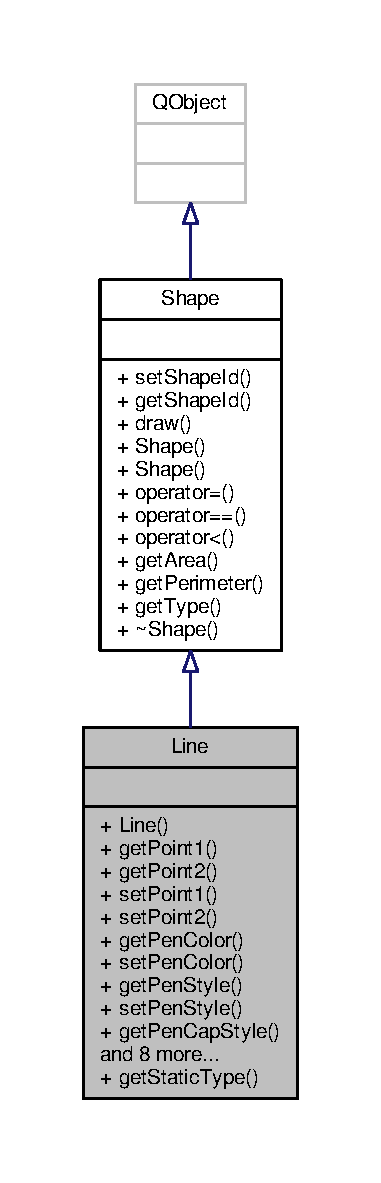
\includegraphics[height=550pt]{classLine__inherit__graph}
\end{center}
\end{figure}


Collaboration diagram for Line\+:\nopagebreak
\begin{figure}[H]
\begin{center}
\leavevmode
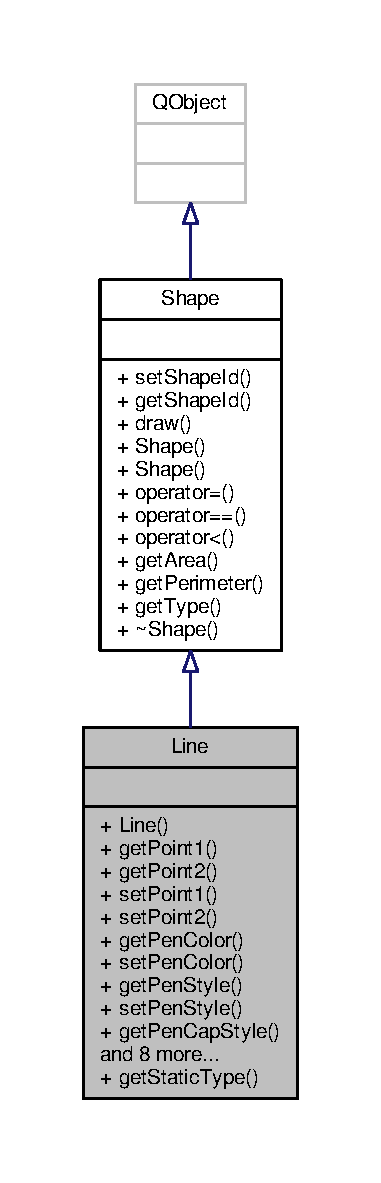
\includegraphics[height=550pt]{classLine__coll__graph}
\end{center}
\end{figure}
\subsection*{Public Member Functions}
\begin{DoxyCompactItemize}
\item 
\hyperlink{classLine_abcc71f5940d76af54fb2a8406418dd44}{Line} (unsigned int, int, int, int, int, Qt\+::\+Global\+Color, Qt\+::\+Pen\+Style, \hyperlink{shape__input__file__specs_8txt_a622efdcfef6789d4367974d2fe79019e}{Qt\+::\+Pen\+Cap\+Style}, \hyperlink{shape__input__file__specs_8txt_a007db2043c6063881de2043c05c9c4a9}{Qt\+::\+Pen\+Join\+Style}, int)
\begin{DoxyCompactList}\small\item\em All parameter constructor for \hyperlink{classLine}{Line}. \end{DoxyCompactList}\item 
Q\+Point \hyperlink{classLine_ad0f6a573ebd8220236e7de8202717f97}{get\+Point1} ()
\begin{DoxyCompactList}\small\item\em Gets the first point of the line. \end{DoxyCompactList}\item 
Q\+Point \hyperlink{classLine_aa64a85c213850620e2ca3df153fe7846}{get\+Point2} ()
\begin{DoxyCompactList}\small\item\em Gets the second point of the line. \end{DoxyCompactList}\item 
void \hyperlink{classLine_a671e977e9b5cb104016def1e9e99c5aa}{set\+Point1} (Q\+Point p1)
\begin{DoxyCompactList}\small\item\em Sets the first point to the given point. \end{DoxyCompactList}\item 
void \hyperlink{classLine_acd4ccc2b472817c45f52297c99a8cbf9}{set\+Point2} (Q\+Point p2)
\begin{DoxyCompactList}\small\item\em Sets the second point to the given point. \end{DoxyCompactList}\item 
Qt\+::\+Global\+Color \hyperlink{classLine_a2d9f0fdcc2da8a29ba39660579150863}{get\+Pen\+Color} ()
\begin{DoxyCompactList}\small\item\em Gets the pen color stored in this shape. \end{DoxyCompactList}\item 
void \hyperlink{classLine_a22f3c1710429e1dd2e883562feba090e}{set\+Pen\+Color} (Qt\+::\+Global\+Color pc)
\begin{DoxyCompactList}\small\item\em Sets the color of the pen to the given color. \end{DoxyCompactList}\item 
Qt\+::\+Pen\+Style \hyperlink{classLine_ab461e7db1a107472e97af08183fccc19}{get\+Pen\+Style} ()
\begin{DoxyCompactList}\small\item\em Gets the style of the pen stored in the shape. \end{DoxyCompactList}\item 
void \hyperlink{classLine_ad0c29864440d59e221d4e4af1c3f2899}{set\+Pen\+Style} (Qt\+::\+Pen\+Style ps)
\begin{DoxyCompactList}\small\item\em Sets the style of the pen to the given style. \end{DoxyCompactList}\item 
\hyperlink{shape__input__file__specs_8txt_a622efdcfef6789d4367974d2fe79019e}{Qt\+::\+Pen\+Cap\+Style} \hyperlink{classLine_afee8c712228659e647752e7198d6891c}{get\+Pen\+Cap\+Style} ()
\begin{DoxyCompactList}\small\item\em Gets the pen cap style that is stored in this \hyperlink{classShape}{Shape}. \end{DoxyCompactList}\item 
void \hyperlink{classLine_a2a3fa8792f5f8e582a6cb902514fcc9c}{set\+Pen\+Cap\+Style} (\hyperlink{shape__input__file__specs_8txt_a622efdcfef6789d4367974d2fe79019e}{Qt\+::\+Pen\+Cap\+Style} pcs)
\begin{DoxyCompactList}\small\item\em Sets the Pen Cap Style to the given Pen Cap Style. \end{DoxyCompactList}\item 
\hyperlink{shape__input__file__specs_8txt_a007db2043c6063881de2043c05c9c4a9}{Qt\+::\+Pen\+Join\+Style} \hyperlink{classLine_a070564edc368231e089c8275ccc2e72d}{get\+Pen\+Join\+Style} ()
\begin{DoxyCompactList}\small\item\em Gets the Pen Join Style. \end{DoxyCompactList}\item 
void \hyperlink{classLine_ae996ba09d0e9c4d06360955486b00f84}{set\+Pen\+Join\+Style} (\hyperlink{shape__input__file__specs_8txt_a007db2043c6063881de2043c05c9c4a9}{Qt\+::\+Pen\+Join\+Style} pjs)
\begin{DoxyCompactList}\small\item\em Sets the pen join style to the given style. \end{DoxyCompactList}\item 
int \hyperlink{classLine_aedbb24685047a4f591fab1b8b7d39125}{get\+Pen\+Width} ()
\begin{DoxyCompactList}\small\item\em Gets the width of the pen. \end{DoxyCompactList}\item 
void \hyperlink{classLine_ade580b43a443e60b77bef50ae98493a2}{set\+Pen\+Width} (int pw)
\begin{DoxyCompactList}\small\item\em Sets the width of the pen to the given width. \end{DoxyCompactList}\item 
virtual void \hyperlink{classLine_a3bcbb11a1d79a7f9a60cc1aac3ab1bb5}{draw} (Q\+Painter \&paint, bool)
\begin{DoxyCompactList}\small\item\em Virtual function to draw shapes. \end{DoxyCompactList}\item 
virtual int \hyperlink{classLine_a249b46f2c7dab063ac4754dbae444468}{get\+Type} ()
\begin{DoxyCompactList}\small\item\em Gets the type of the shape. \end{DoxyCompactList}\item 
virtual double \hyperlink{classLine_ad63a55614d118000935e585f3551f630}{get\+Perimeter} ()
\begin{DoxyCompactList}\small\item\em Gets the perimeter of the given shape. \end{DoxyCompactList}\end{DoxyCompactItemize}
\subsection*{Static Public Member Functions}
\begin{DoxyCompactItemize}
\item 
static int \hyperlink{classLine_aec5465504d5c944920fd96a7d81c8472}{get\+Static\+Type} ()
\begin{DoxyCompactList}\small\item\em gets the Type of object \end{DoxyCompactList}\end{DoxyCompactItemize}


\subsection{Detailed Description}
\hyperlink{classLine}{Line} class that Q\+Painter can draw. 

\subsection{Constructor \& Destructor Documentation}
\index{Line@{Line}!Line@{Line}}
\index{Line@{Line}!Line@{Line}}
\subsubsection[{\texorpdfstring{Line(unsigned int, int, int, int, int, Qt\+::\+Global\+Color, Qt\+::\+Pen\+Style, Qt\+::\+Pen\+Cap\+Style, Qt\+::\+Pen\+Join\+Style, int)}{Line(unsigned int, int, int, int, int, Qt::GlobalColor, Qt::PenStyle, Qt::PenCapStyle, Qt::PenJoinStyle, int)}}]{\setlength{\rightskip}{0pt plus 5cm}Line\+::\+Line (
\begin{DoxyParamCaption}
\item[{unsigned int}]{i, }
\item[{int}]{x1, }
\item[{int}]{y1, }
\item[{int}]{x2, }
\item[{int}]{y2, }
\item[{Qt\+::\+Global\+Color}]{pc, }
\item[{Qt\+::\+Pen\+Style}]{ps, }
\item[{{\bf Qt\+::\+Pen\+Cap\+Style}}]{pcs, }
\item[{{\bf Qt\+::\+Pen\+Join\+Style}}]{pjs, }
\item[{int}]{pw}
\end{DoxyParamCaption}
)}\hypertarget{classLine_abcc71f5940d76af54fb2a8406418dd44}{}\label{classLine_abcc71f5940d76af54fb2a8406418dd44}


All parameter constructor for \hyperlink{classLine}{Line}. 



\subsection{Member Function Documentation}
\index{Line@{Line}!draw@{draw}}
\index{draw@{draw}!Line@{Line}}
\subsubsection[{\texorpdfstring{draw(\+Q\+Painter \&paint, bool)}{draw(QPainter &paint, bool)}}]{\setlength{\rightskip}{0pt plus 5cm}void Line\+::draw (
\begin{DoxyParamCaption}
\item[{Q\+Painter \&}]{, }
\item[{bool}]{}
\end{DoxyParamCaption}
)\hspace{0.3cm}{\ttfamily [virtual]}}\hypertarget{classLine_a3bcbb11a1d79a7f9a60cc1aac3ab1bb5}{}\label{classLine_a3bcbb11a1d79a7f9a60cc1aac3ab1bb5}


Virtual function to draw shapes. 



Implements \hyperlink{classShape_a47dae32819e64fb32f3357f31978293f}{Shape}.

\index{Line@{Line}!get\+Pen\+Cap\+Style@{get\+Pen\+Cap\+Style}}
\index{get\+Pen\+Cap\+Style@{get\+Pen\+Cap\+Style}!Line@{Line}}
\subsubsection[{\texorpdfstring{get\+Pen\+Cap\+Style()}{getPenCapStyle()}}]{\setlength{\rightskip}{0pt plus 5cm}{\bf Qt\+::\+Pen\+Cap\+Style} Line\+::get\+Pen\+Cap\+Style (
\begin{DoxyParamCaption}
{}
\end{DoxyParamCaption}
)\hspace{0.3cm}{\ttfamily [inline]}}\hypertarget{classLine_afee8c712228659e647752e7198d6891c}{}\label{classLine_afee8c712228659e647752e7198d6891c}


Gets the pen cap style that is stored in this \hyperlink{classShape}{Shape}. 

\begin{DoxyReturn}{Returns}
Pen\+Cap\+Style 
\end{DoxyReturn}
\index{Line@{Line}!get\+Pen\+Color@{get\+Pen\+Color}}
\index{get\+Pen\+Color@{get\+Pen\+Color}!Line@{Line}}
\subsubsection[{\texorpdfstring{get\+Pen\+Color()}{getPenColor()}}]{\setlength{\rightskip}{0pt plus 5cm}Qt\+::\+Global\+Color Line\+::get\+Pen\+Color (
\begin{DoxyParamCaption}
{}
\end{DoxyParamCaption}
)\hspace{0.3cm}{\ttfamily [inline]}}\hypertarget{classLine_a2d9f0fdcc2da8a29ba39660579150863}{}\label{classLine_a2d9f0fdcc2da8a29ba39660579150863}


Gets the pen color stored in this shape. 

\begin{DoxyReturn}{Returns}
Color of the pen 
\end{DoxyReturn}
\index{Line@{Line}!get\+Pen\+Join\+Style@{get\+Pen\+Join\+Style}}
\index{get\+Pen\+Join\+Style@{get\+Pen\+Join\+Style}!Line@{Line}}
\subsubsection[{\texorpdfstring{get\+Pen\+Join\+Style()}{getPenJoinStyle()}}]{\setlength{\rightskip}{0pt plus 5cm}{\bf Qt\+::\+Pen\+Join\+Style} Line\+::get\+Pen\+Join\+Style (
\begin{DoxyParamCaption}
{}
\end{DoxyParamCaption}
)\hspace{0.3cm}{\ttfamily [inline]}}\hypertarget{classLine_a070564edc368231e089c8275ccc2e72d}{}\label{classLine_a070564edc368231e089c8275ccc2e72d}


Gets the Pen Join Style. 

\begin{DoxyReturn}{Returns}
Pen\+Join\+Style 
\end{DoxyReturn}
\index{Line@{Line}!get\+Pen\+Style@{get\+Pen\+Style}}
\index{get\+Pen\+Style@{get\+Pen\+Style}!Line@{Line}}
\subsubsection[{\texorpdfstring{get\+Pen\+Style()}{getPenStyle()}}]{\setlength{\rightskip}{0pt plus 5cm}Qt\+::\+Pen\+Style Line\+::get\+Pen\+Style (
\begin{DoxyParamCaption}
{}
\end{DoxyParamCaption}
)\hspace{0.3cm}{\ttfamily [inline]}}\hypertarget{classLine_ab461e7db1a107472e97af08183fccc19}{}\label{classLine_ab461e7db1a107472e97af08183fccc19}


Gets the style of the pen stored in the shape. 

\begin{DoxyReturn}{Returns}
Style of the pen 
\end{DoxyReturn}
\index{Line@{Line}!get\+Pen\+Width@{get\+Pen\+Width}}
\index{get\+Pen\+Width@{get\+Pen\+Width}!Line@{Line}}
\subsubsection[{\texorpdfstring{get\+Pen\+Width()}{getPenWidth()}}]{\setlength{\rightskip}{0pt plus 5cm}int Line\+::get\+Pen\+Width (
\begin{DoxyParamCaption}
{}
\end{DoxyParamCaption}
)\hspace{0.3cm}{\ttfamily [inline]}}\hypertarget{classLine_aedbb24685047a4f591fab1b8b7d39125}{}\label{classLine_aedbb24685047a4f591fab1b8b7d39125}


Gets the width of the pen. 

\begin{DoxyReturn}{Returns}
pen\+Width 
\end{DoxyReturn}
\index{Line@{Line}!get\+Perimeter@{get\+Perimeter}}
\index{get\+Perimeter@{get\+Perimeter}!Line@{Line}}
\subsubsection[{\texorpdfstring{get\+Perimeter()}{getPerimeter()}}]{\setlength{\rightskip}{0pt plus 5cm}virtual double Line\+::get\+Perimeter (
\begin{DoxyParamCaption}
{}
\end{DoxyParamCaption}
)\hspace{0.3cm}{\ttfamily [inline]}, {\ttfamily [virtual]}}\hypertarget{classLine_ad63a55614d118000935e585f3551f630}{}\label{classLine_ad63a55614d118000935e585f3551f630}


Gets the perimeter of the given shape. 

\begin{DoxyReturn}{Returns}
Perimeter as a double 
\end{DoxyReturn}


Reimplemented from \hyperlink{classShape_a391744b6bce96df044139dcbd1ae0aa8}{Shape}.

\index{Line@{Line}!get\+Point1@{get\+Point1}}
\index{get\+Point1@{get\+Point1}!Line@{Line}}
\subsubsection[{\texorpdfstring{get\+Point1()}{getPoint1()}}]{\setlength{\rightskip}{0pt plus 5cm}Q\+Point Line\+::get\+Point1 (
\begin{DoxyParamCaption}
{}
\end{DoxyParamCaption}
)\hspace{0.3cm}{\ttfamily [inline]}}\hypertarget{classLine_ad0f6a573ebd8220236e7de8202717f97}{}\label{classLine_ad0f6a573ebd8220236e7de8202717f97}


Gets the first point of the line. 

\begin{DoxyReturn}{Returns}
Q\+Point of the first point 
\end{DoxyReturn}
\index{Line@{Line}!get\+Point2@{get\+Point2}}
\index{get\+Point2@{get\+Point2}!Line@{Line}}
\subsubsection[{\texorpdfstring{get\+Point2()}{getPoint2()}}]{\setlength{\rightskip}{0pt plus 5cm}Q\+Point Line\+::get\+Point2 (
\begin{DoxyParamCaption}
{}
\end{DoxyParamCaption}
)\hspace{0.3cm}{\ttfamily [inline]}}\hypertarget{classLine_aa64a85c213850620e2ca3df153fe7846}{}\label{classLine_aa64a85c213850620e2ca3df153fe7846}


Gets the second point of the line. 

\begin{DoxyReturn}{Returns}
Q\+Point of the second point 
\end{DoxyReturn}
\index{Line@{Line}!get\+Static\+Type@{get\+Static\+Type}}
\index{get\+Static\+Type@{get\+Static\+Type}!Line@{Line}}
\subsubsection[{\texorpdfstring{get\+Static\+Type()}{getStaticType()}}]{\setlength{\rightskip}{0pt plus 5cm}static int Line\+::get\+Static\+Type (
\begin{DoxyParamCaption}
{}
\end{DoxyParamCaption}
)\hspace{0.3cm}{\ttfamily [inline]}, {\ttfamily [static]}}\hypertarget{classLine_aec5465504d5c944920fd96a7d81c8472}{}\label{classLine_aec5465504d5c944920fd96a7d81c8472}


gets the Type of object 

\begin{DoxyReturn}{Returns}
Type as int 
\end{DoxyReturn}
\index{Line@{Line}!get\+Type@{get\+Type}}
\index{get\+Type@{get\+Type}!Line@{Line}}
\subsubsection[{\texorpdfstring{get\+Type()}{getType()}}]{\setlength{\rightskip}{0pt plus 5cm}virtual int Line\+::get\+Type (
\begin{DoxyParamCaption}
{}
\end{DoxyParamCaption}
)\hspace{0.3cm}{\ttfamily [inline]}, {\ttfamily [virtual]}}\hypertarget{classLine_a249b46f2c7dab063ac4754dbae444468}{}\label{classLine_a249b46f2c7dab063ac4754dbae444468}


Gets the type of the shape. 

\begin{DoxyReturn}{Returns}
type as an int 
\end{DoxyReturn}


Implements \hyperlink{classShape_a3d15adf2a1d746928f9be98105096eda}{Shape}.

\index{Line@{Line}!set\+Pen\+Cap\+Style@{set\+Pen\+Cap\+Style}}
\index{set\+Pen\+Cap\+Style@{set\+Pen\+Cap\+Style}!Line@{Line}}
\subsubsection[{\texorpdfstring{set\+Pen\+Cap\+Style(\+Qt\+::\+Pen\+Cap\+Style pcs)}{setPenCapStyle(Qt::PenCapStyle pcs)}}]{\setlength{\rightskip}{0pt plus 5cm}void Line\+::set\+Pen\+Cap\+Style (
\begin{DoxyParamCaption}
\item[{{\bf Qt\+::\+Pen\+Cap\+Style}}]{pcs}
\end{DoxyParamCaption}
)\hspace{0.3cm}{\ttfamily [inline]}}\hypertarget{classLine_a2a3fa8792f5f8e582a6cb902514fcc9c}{}\label{classLine_a2a3fa8792f5f8e582a6cb902514fcc9c}


Sets the Pen Cap Style to the given Pen Cap Style. 


\begin{DoxyParams}{Parameters}
{\em pen\+Cap\+Style} & \\
\hline
\end{DoxyParams}
\index{Line@{Line}!set\+Pen\+Color@{set\+Pen\+Color}}
\index{set\+Pen\+Color@{set\+Pen\+Color}!Line@{Line}}
\subsubsection[{\texorpdfstring{set\+Pen\+Color(\+Qt\+::\+Global\+Color pc)}{setPenColor(Qt::GlobalColor pc)}}]{\setlength{\rightskip}{0pt plus 5cm}void Line\+::set\+Pen\+Color (
\begin{DoxyParamCaption}
\item[{Qt\+::\+Global\+Color}]{pc}
\end{DoxyParamCaption}
)\hspace{0.3cm}{\ttfamily [inline]}}\hypertarget{classLine_a22f3c1710429e1dd2e883562feba090e}{}\label{classLine_a22f3c1710429e1dd2e883562feba090e}


Sets the color of the pen to the given color. 


\begin{DoxyParams}{Parameters}
{\em pen\+Color} & \\
\hline
\end{DoxyParams}
\index{Line@{Line}!set\+Pen\+Join\+Style@{set\+Pen\+Join\+Style}}
\index{set\+Pen\+Join\+Style@{set\+Pen\+Join\+Style}!Line@{Line}}
\subsubsection[{\texorpdfstring{set\+Pen\+Join\+Style(\+Qt\+::\+Pen\+Join\+Style pjs)}{setPenJoinStyle(Qt::PenJoinStyle pjs)}}]{\setlength{\rightskip}{0pt plus 5cm}void Line\+::set\+Pen\+Join\+Style (
\begin{DoxyParamCaption}
\item[{{\bf Qt\+::\+Pen\+Join\+Style}}]{pjs}
\end{DoxyParamCaption}
)\hspace{0.3cm}{\ttfamily [inline]}}\hypertarget{classLine_ae996ba09d0e9c4d06360955486b00f84}{}\label{classLine_ae996ba09d0e9c4d06360955486b00f84}


Sets the pen join style to the given style. 


\begin{DoxyParams}{Parameters}
{\em pen\+Join\+Style} & \\
\hline
\end{DoxyParams}
\index{Line@{Line}!set\+Pen\+Style@{set\+Pen\+Style}}
\index{set\+Pen\+Style@{set\+Pen\+Style}!Line@{Line}}
\subsubsection[{\texorpdfstring{set\+Pen\+Style(\+Qt\+::\+Pen\+Style ps)}{setPenStyle(Qt::PenStyle ps)}}]{\setlength{\rightskip}{0pt plus 5cm}void Line\+::set\+Pen\+Style (
\begin{DoxyParamCaption}
\item[{Qt\+::\+Pen\+Style}]{ps}
\end{DoxyParamCaption}
)\hspace{0.3cm}{\ttfamily [inline]}}\hypertarget{classLine_ad0c29864440d59e221d4e4af1c3f2899}{}\label{classLine_ad0c29864440d59e221d4e4af1c3f2899}


Sets the style of the pen to the given style. 


\begin{DoxyParams}{Parameters}
{\em pen\+Style} & \\
\hline
\end{DoxyParams}
\index{Line@{Line}!set\+Pen\+Width@{set\+Pen\+Width}}
\index{set\+Pen\+Width@{set\+Pen\+Width}!Line@{Line}}
\subsubsection[{\texorpdfstring{set\+Pen\+Width(int pw)}{setPenWidth(int pw)}}]{\setlength{\rightskip}{0pt plus 5cm}void Line\+::set\+Pen\+Width (
\begin{DoxyParamCaption}
\item[{int}]{pw}
\end{DoxyParamCaption}
)\hspace{0.3cm}{\ttfamily [inline]}}\hypertarget{classLine_ade580b43a443e60b77bef50ae98493a2}{}\label{classLine_ade580b43a443e60b77bef50ae98493a2}


Sets the width of the pen to the given width. 


\begin{DoxyParams}{Parameters}
{\em pen\+Width} & \\
\hline
\end{DoxyParams}
\index{Line@{Line}!set\+Point1@{set\+Point1}}
\index{set\+Point1@{set\+Point1}!Line@{Line}}
\subsubsection[{\texorpdfstring{set\+Point1(\+Q\+Point p1)}{setPoint1(QPoint p1)}}]{\setlength{\rightskip}{0pt plus 5cm}void Line\+::set\+Point1 (
\begin{DoxyParamCaption}
\item[{Q\+Point}]{p1}
\end{DoxyParamCaption}
)\hspace{0.3cm}{\ttfamily [inline]}}\hypertarget{classLine_a671e977e9b5cb104016def1e9e99c5aa}{}\label{classLine_a671e977e9b5cb104016def1e9e99c5aa}


Sets the first point to the given point. 


\begin{DoxyParams}{Parameters}
{\em Q\+Point} & for the first point \\
\hline
\end{DoxyParams}
\index{Line@{Line}!set\+Point2@{set\+Point2}}
\index{set\+Point2@{set\+Point2}!Line@{Line}}
\subsubsection[{\texorpdfstring{set\+Point2(\+Q\+Point p2)}{setPoint2(QPoint p2)}}]{\setlength{\rightskip}{0pt plus 5cm}void Line\+::set\+Point2 (
\begin{DoxyParamCaption}
\item[{Q\+Point}]{p2}
\end{DoxyParamCaption}
)\hspace{0.3cm}{\ttfamily [inline]}}\hypertarget{classLine_acd4ccc2b472817c45f52297c99a8cbf9}{}\label{classLine_acd4ccc2b472817c45f52297c99a8cbf9}


Sets the second point to the given point. 


\begin{DoxyParams}{Parameters}
{\em Q\+Point} & of the second point \\
\hline
\end{DoxyParams}


The documentation for this class was generated from the following files\+:\begin{DoxyCompactItemize}
\item 
Group Project/\+Scrum\+Of\+The\+Earth/\hyperlink{line_8h}{line.\+h}\item 
Group Project/\+Scrum\+Of\+The\+Earth/\hyperlink{line_8cpp}{line.\+cpp}\end{DoxyCompactItemize}

\hypertarget{classMainWindow}{}\section{Main\+Window Class Reference}
\label{classMainWindow}\index{Main\+Window@{Main\+Window}}


The \hyperlink{classMainWindow}{Main\+Window} class provides the environment for the \hyperlink{classRenderArea}{Render\+Area}, Tables, and Buttons.  




{\ttfamily \#include $<$mainwindow.\+h$>$}



Inheritance diagram for Main\+Window\+:\nopagebreak
\begin{figure}[H]
\begin{center}
\leavevmode
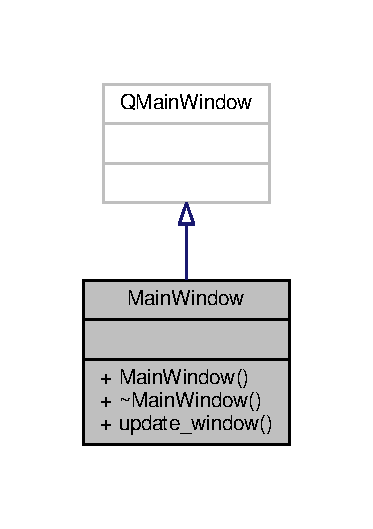
\includegraphics[width=179pt]{classMainWindow__inherit__graph}
\end{center}
\end{figure}


Collaboration diagram for Main\+Window\+:\nopagebreak
\begin{figure}[H]
\begin{center}
\leavevmode
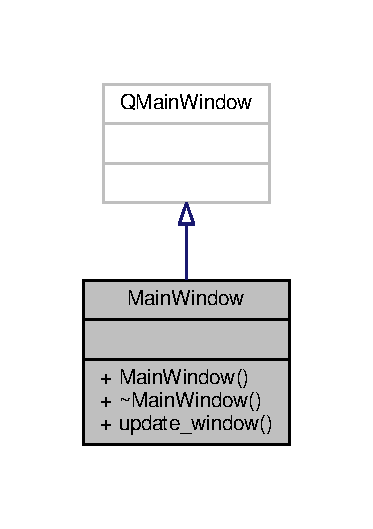
\includegraphics[width=179pt]{classMainWindow__coll__graph}
\end{center}
\end{figure}
\subsection*{Public Slots}
\begin{DoxyCompactItemize}
\item 
void \hyperlink{classMainWindow_a59351bdf1235b640a416121e7b8d89d3}{update\+\_\+window} ()
\begin{DoxyCompactList}\small\item\em Slot update\+\_\+window updates the render area and the tables from its vector. \end{DoxyCompactList}\end{DoxyCompactItemize}
\subsection*{Public Member Functions}
\begin{DoxyCompactItemize}
\item 
\hyperlink{classMainWindow_a16bf19588e7e7cb601b4e01661a9141b}{Main\+Window} (Q\+Widget $\ast$parent=nullptr, bool admin=false)
\begin{DoxyCompactList}\small\item\em \hyperlink{classMainWindow}{Main\+Window} constructor. \end{DoxyCompactList}\item 
\hyperlink{classMainWindow_ae98d00a93bc118200eeef9f9bba1dba7}{$\sim$\+Main\+Window} ()
\begin{DoxyCompactList}\small\item\em \hyperlink{classMainWindow}{Main\+Window} Destructor. \end{DoxyCompactList}\end{DoxyCompactItemize}


\subsection{Detailed Description}
The \hyperlink{classMainWindow}{Main\+Window} class provides the environment for the \hyperlink{classRenderArea}{Render\+Area}, Tables, and Buttons. 

\subsection{Constructor \& Destructor Documentation}
\index{Main\+Window@{Main\+Window}!Main\+Window@{Main\+Window}}
\index{Main\+Window@{Main\+Window}!Main\+Window@{Main\+Window}}
\subsubsection[{\texorpdfstring{Main\+Window(\+Q\+Widget $\ast$parent=nullptr, bool admin=false)}{MainWindow(QWidget *parent=nullptr, bool admin=false)}}]{\setlength{\rightskip}{0pt plus 5cm}Main\+Window\+::\+Main\+Window (
\begin{DoxyParamCaption}
\item[{Q\+Widget $\ast$}]{parent = {\ttfamily nullptr}, }
\item[{bool}]{admin = {\ttfamily false}}
\end{DoxyParamCaption}
)\hspace{0.3cm}{\ttfamily [explicit]}}\hypertarget{classMainWindow_a16bf19588e7e7cb601b4e01661a9141b}{}\label{classMainWindow_a16bf19588e7e7cb601b4e01661a9141b}


\hyperlink{classMainWindow}{Main\+Window} constructor. 


\begin{DoxyParams}{Parameters}
{\em parent} & window \\
\hline
{\em admin} & bool \\
\hline
\end{DoxyParams}
\index{Main\+Window@{Main\+Window}!````~Main\+Window@{$\sim$\+Main\+Window}}
\index{````~Main\+Window@{$\sim$\+Main\+Window}!Main\+Window@{Main\+Window}}
\subsubsection[{\texorpdfstring{$\sim$\+Main\+Window()}{~MainWindow()}}]{\setlength{\rightskip}{0pt plus 5cm}Main\+Window\+::$\sim$\+Main\+Window (
\begin{DoxyParamCaption}
{}
\end{DoxyParamCaption}
)}\hypertarget{classMainWindow_ae98d00a93bc118200eeef9f9bba1dba7}{}\label{classMainWindow_ae98d00a93bc118200eeef9f9bba1dba7}


\hyperlink{classMainWindow}{Main\+Window} Destructor. 



\subsection{Member Function Documentation}
\index{Main\+Window@{Main\+Window}!update\+\_\+window@{update\+\_\+window}}
\index{update\+\_\+window@{update\+\_\+window}!Main\+Window@{Main\+Window}}
\subsubsection[{\texorpdfstring{update\+\_\+window}{update_window}}]{\setlength{\rightskip}{0pt plus 5cm}void Main\+Window\+::update\+\_\+window (
\begin{DoxyParamCaption}
{}
\end{DoxyParamCaption}
)\hspace{0.3cm}{\ttfamily [slot]}}\hypertarget{classMainWindow_a59351bdf1235b640a416121e7b8d89d3}{}\label{classMainWindow_a59351bdf1235b640a416121e7b8d89d3}


Slot update\+\_\+window updates the render area and the tables from its vector. 



The documentation for this class was generated from the following files\+:\begin{DoxyCompactItemize}
\item 
Group Project/\+Scrum\+Of\+The\+Earth/\hyperlink{mainwindow_8h}{mainwindow.\+h}\item 
Group Project/\+Scrum\+Of\+The\+Earth/\hyperlink{mainwindow_8cpp}{mainwindow.\+cpp}\end{DoxyCompactItemize}

\hypertarget{classMoveShape}{}\section{Move\+Shape Class Reference}
\label{classMoveShape}\index{Move\+Shape@{Move\+Shape}}


The \hyperlink{classMoveShape}{Move\+Shape} class provides the interface and functionality for moving shapes.  




{\ttfamily \#include $<$moveshape.\+h$>$}



Inheritance diagram for Move\+Shape\+:\nopagebreak
\begin{figure}[H]
\begin{center}
\leavevmode
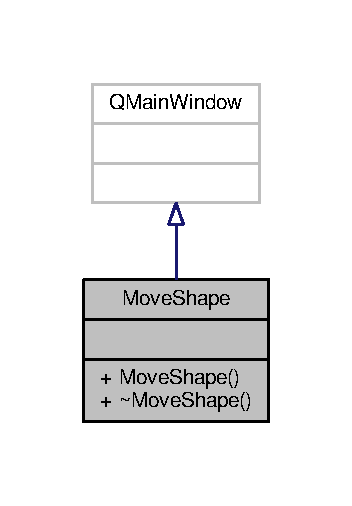
\includegraphics[width=169pt]{classMoveShape__inherit__graph}
\end{center}
\end{figure}


Collaboration diagram for Move\+Shape\+:\nopagebreak
\begin{figure}[H]
\begin{center}
\leavevmode
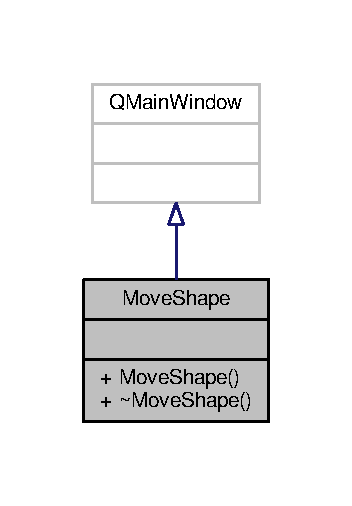
\includegraphics[width=169pt]{classMoveShape__coll__graph}
\end{center}
\end{figure}
\subsection*{Signals}
\begin{DoxyCompactItemize}
\item 
void \hyperlink{classMoveShape_a020f54b76f345cc9fa83ba8deb4af9c6}{update\+\_\+win} ()
\begin{DoxyCompactList}\small\item\em Updates window whenever a shape is added. \end{DoxyCompactList}\end{DoxyCompactItemize}
\subsection*{Public Member Functions}
\begin{DoxyCompactItemize}
\item 
\hyperlink{classMoveShape_a475fca3688eb29093886a0508f8e9b83}{Move\+Shape} (Q\+Widget $\ast$parent, \hyperlink{classmyStd_1_1vector}{my\+Std\+::vector}$<$ \hyperlink{classShape}{Shape} $\ast$ $>$ \&shapes)
\begin{DoxyCompactList}\small\item\em \hyperlink{classMoveShape}{Move\+Shape} constructor. \end{DoxyCompactList}\item 
\hyperlink{classMoveShape_a9790764b1e1ec53da191338e6fa763ac}{$\sim$\+Move\+Shape} ()
\end{DoxyCompactItemize}


\subsection{Detailed Description}
The \hyperlink{classMoveShape}{Move\+Shape} class provides the interface and functionality for moving shapes. 

\subsection{Constructor \& Destructor Documentation}
\index{Move\+Shape@{Move\+Shape}!Move\+Shape@{Move\+Shape}}
\index{Move\+Shape@{Move\+Shape}!Move\+Shape@{Move\+Shape}}
\subsubsection[{\texorpdfstring{Move\+Shape(\+Q\+Widget $\ast$parent, my\+Std\+::vector$<$ Shape $\ast$ $>$ \&shapes)}{MoveShape(QWidget *parent, myStd::vector< Shape * > &shapes)}}]{\setlength{\rightskip}{0pt plus 5cm}Move\+Shape\+::\+Move\+Shape (
\begin{DoxyParamCaption}
\item[{Q\+Widget $\ast$}]{parent, }
\item[{{\bf my\+Std\+::vector}$<$ {\bf Shape} $\ast$ $>$ \&}]{shapes}
\end{DoxyParamCaption}
)\hspace{0.3cm}{\ttfamily [explicit]}}\hypertarget{classMoveShape_a475fca3688eb29093886a0508f8e9b83}{}\label{classMoveShape_a475fca3688eb29093886a0508f8e9b83}


\hyperlink{classMoveShape}{Move\+Shape} constructor. 


\begin{DoxyParams}{Parameters}
{\em parent} & window \\
\hline
{\em shapes} & pointer vector \\
\hline
\end{DoxyParams}
\index{Move\+Shape@{Move\+Shape}!````~Move\+Shape@{$\sim$\+Move\+Shape}}
\index{````~Move\+Shape@{$\sim$\+Move\+Shape}!Move\+Shape@{Move\+Shape}}
\subsubsection[{\texorpdfstring{$\sim$\+Move\+Shape()}{~MoveShape()}}]{\setlength{\rightskip}{0pt plus 5cm}Move\+Shape\+::$\sim$\+Move\+Shape (
\begin{DoxyParamCaption}
{}
\end{DoxyParamCaption}
)}\hypertarget{classMoveShape_a9790764b1e1ec53da191338e6fa763ac}{}\label{classMoveShape_a9790764b1e1ec53da191338e6fa763ac}


\subsection{Member Function Documentation}
\index{Move\+Shape@{Move\+Shape}!update\+\_\+win@{update\+\_\+win}}
\index{update\+\_\+win@{update\+\_\+win}!Move\+Shape@{Move\+Shape}}
\subsubsection[{\texorpdfstring{update\+\_\+win}{update_win}}]{\setlength{\rightskip}{0pt plus 5cm}void Move\+Shape\+::update\+\_\+win (
\begin{DoxyParamCaption}
{}
\end{DoxyParamCaption}
)\hspace{0.3cm}{\ttfamily [signal]}}\hypertarget{classMoveShape_a020f54b76f345cc9fa83ba8deb4af9c6}{}\label{classMoveShape_a020f54b76f345cc9fa83ba8deb4af9c6}


Updates window whenever a shape is added. 



The documentation for this class was generated from the following files\+:\begin{DoxyCompactItemize}
\item 
Group Project/\+Scrum\+Of\+The\+Earth/\hyperlink{moveshape_8h}{moveshape.\+h}\item 
Group Project/\+Scrum\+Of\+The\+Earth/\hyperlink{moveshape_8cpp}{moveshape.\+cpp}\end{DoxyCompactItemize}

\hypertarget{classPolygon}{}\section{Polygon Class Reference}
\label{classPolygon}\index{Polygon@{Polygon}}


\hyperlink{classPolygon}{Polygon} class that Q\+Painter can draw.  




{\ttfamily \#include $<$polygon.\+h$>$}



Inheritance diagram for Polygon\+:\nopagebreak
\begin{figure}[H]
\begin{center}
\leavevmode
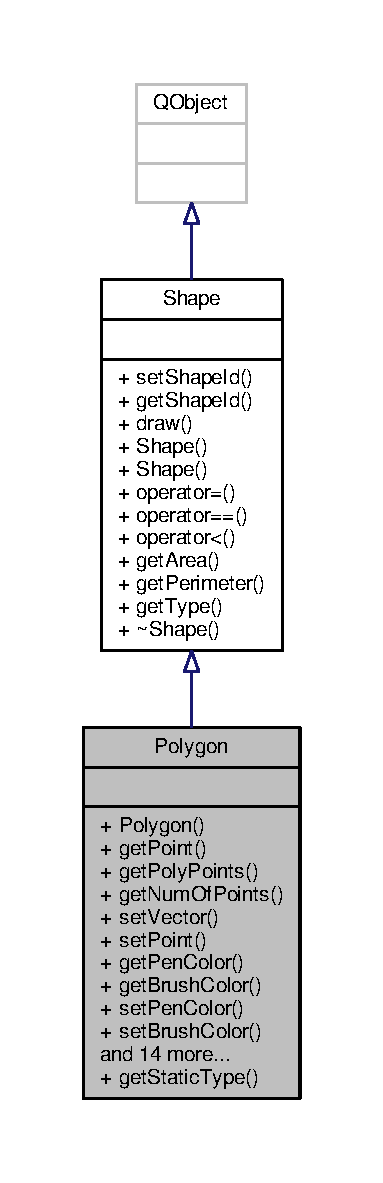
\includegraphics[height=550pt]{classPolygon__inherit__graph}
\end{center}
\end{figure}


Collaboration diagram for Polygon\+:\nopagebreak
\begin{figure}[H]
\begin{center}
\leavevmode
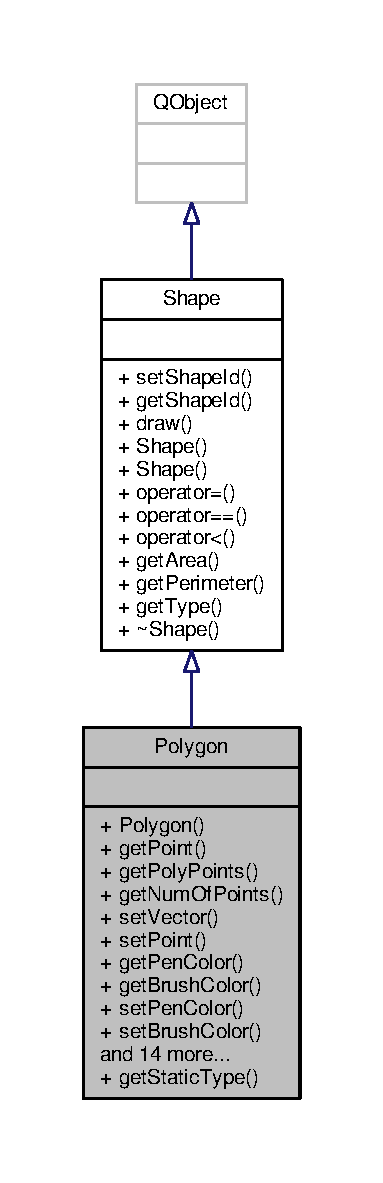
\includegraphics[height=550pt]{classPolygon__coll__graph}
\end{center}
\end{figure}
\subsection*{Public Member Functions}
\begin{DoxyCompactItemize}
\item 
\hyperlink{classPolygon_ad85ab576e63cdafd2d0a821a7cebd40a}{Polygon} (unsigned int, \hyperlink{classmyStd_1_1vector}{my\+Std\+::vector}$<$ Q\+Point $>$, Qt\+::\+Global\+Color, Qt\+::\+Global\+Color, Qt\+::\+Pen\+Style, \hyperlink{shape__input__file__specs_8txt_a622efdcfef6789d4367974d2fe79019e}{Qt\+::\+Pen\+Cap\+Style}, \hyperlink{shape__input__file__specs_8txt_a007db2043c6063881de2043c05c9c4a9}{Qt\+::\+Pen\+Join\+Style}, \hyperlink{shape__input__file__specs_8txt_ad07f6fe6c28dcb0b3bdc324a72d0051f}{Qt\+::\+Brush\+Style}, int)
\begin{DoxyCompactList}\small\item\em All parameter constructor. \end{DoxyCompactList}\item 
Q\+Point \hyperlink{classPolygon_ad7e1a7964733cb80b095b7dd66fb0551}{get\+Point} (int i)
\begin{DoxyCompactList}\small\item\em Gets the i-\/th point of the polygon. \end{DoxyCompactList}\item 
Q\+Point $\ast$ \hyperlink{classPolygon_a254935fca8f07c8b337ae96e19283464}{get\+Poly\+Points} ()
\begin{DoxyCompactList}\small\item\em Gets an array of Q\+Points that contain the corners of the polygon. \end{DoxyCompactList}\item 
int \hyperlink{classPolygon_aaa21d89b5cdf770f421d19524e82734c}{get\+Num\+Of\+Points} ()
\begin{DoxyCompactList}\small\item\em Gets the number of points. \end{DoxyCompactList}\item 
void \hyperlink{classPolygon_aa7f5e838167b0c1b57320fd418325b8c}{set\+Vector} (\hyperlink{classmyStd_1_1vector}{my\+Std\+::vector}$<$ Q\+Point $>$ v)
\begin{DoxyCompactList}\small\item\em Sets the vector of Q\+Points to the given vector. \end{DoxyCompactList}\item 
void \hyperlink{classPolygon_a19e111329052166c5eeb2d6933066774}{set\+Point} (Q\+Point p, int i)
\begin{DoxyCompactList}\small\item\em Sets the i-\/th point of the polygon to the given point. \end{DoxyCompactList}\item 
Qt\+::\+Global\+Color \hyperlink{classPolygon_a495a1a0d772def2064a1c19762b769c2}{get\+Pen\+Color} ()
\begin{DoxyCompactList}\small\item\em Gets the pen color stored in this shape. \end{DoxyCompactList}\item 
Qt\+::\+Global\+Color \hyperlink{classPolygon_a201ddc5bb4071243ec497028f70b6d51}{get\+Brush\+Color} ()
\begin{DoxyCompactList}\small\item\em Gets the Brush color stored in the \hyperlink{classShape}{Shape}. \end{DoxyCompactList}\item 
void \hyperlink{classPolygon_aa5e4c1ec34f061e201ab5ff38b55f945}{set\+Pen\+Color} (Qt\+::\+Global\+Color pc)
\begin{DoxyCompactList}\small\item\em Sets the color of the pen to the given color. \end{DoxyCompactList}\item 
void \hyperlink{classPolygon_a09d905fcc1c8fd0b25772d54d1d5c831}{set\+Brush\+Color} (Qt\+::\+Global\+Color bc)
\begin{DoxyCompactList}\small\item\em Sets the color of the Brush to the given color. \end{DoxyCompactList}\item 
Qt\+::\+Pen\+Style \hyperlink{classPolygon_ad17a682e3a31c185086a56ac36b1a732}{get\+Pen\+Style} ()
\begin{DoxyCompactList}\small\item\em Gets the style of the pen stored in the shape. \end{DoxyCompactList}\item 
void \hyperlink{classPolygon_afd47f455b19d368bea8a198d4fcfa81f}{set\+Pen\+Style} (Qt\+::\+Pen\+Style ps)
\begin{DoxyCompactList}\small\item\em Sets the style of the pen to the given style. \end{DoxyCompactList}\item 
\hyperlink{shape__input__file__specs_8txt_a622efdcfef6789d4367974d2fe79019e}{Qt\+::\+Pen\+Cap\+Style} \hyperlink{classPolygon_a6a87aa5a647a925d520fb3462e3450dc}{get\+Pen\+Cap\+Style} ()
\begin{DoxyCompactList}\small\item\em Gets the pen cap style that is stored in this \hyperlink{classShape}{Shape}. \end{DoxyCompactList}\item 
void \hyperlink{classPolygon_a9bffdd7d7b4f98fdb14fcba435ff4857}{set\+Pen\+Cap\+Style} (\hyperlink{shape__input__file__specs_8txt_a622efdcfef6789d4367974d2fe79019e}{Qt\+::\+Pen\+Cap\+Style} pcs)
\begin{DoxyCompactList}\small\item\em Sets the Pen Cap Style to the given Pen Cap Style. \end{DoxyCompactList}\item 
\hyperlink{shape__input__file__specs_8txt_a007db2043c6063881de2043c05c9c4a9}{Qt\+::\+Pen\+Join\+Style} \hyperlink{classPolygon_a1472bbc12cc60b90b666d509ffefaf47}{get\+Pen\+Join\+Style} ()
\begin{DoxyCompactList}\small\item\em Gets the Pen Join Style. \end{DoxyCompactList}\item 
void \hyperlink{classPolygon_a1dbd55cf600447893405712943f01a95}{set\+Pen\+Join\+Style} (\hyperlink{shape__input__file__specs_8txt_a007db2043c6063881de2043c05c9c4a9}{Qt\+::\+Pen\+Join\+Style} pjs)
\begin{DoxyCompactList}\small\item\em Sets the pen join style to the given style. \end{DoxyCompactList}\item 
\hyperlink{shape__input__file__specs_8txt_ad07f6fe6c28dcb0b3bdc324a72d0051f}{Qt\+::\+Brush\+Style} \hyperlink{classPolygon_a8a827f50a6b4f1a3233cc343b26e5bf4}{get\+Brush\+Style} ()
\begin{DoxyCompactList}\small\item\em Gets the Brush Style. \end{DoxyCompactList}\item 
void \hyperlink{classPolygon_a8c373e3f2f22b4e25adc081dfba4c007}{set\+Brush\+Style} (\hyperlink{shape__input__file__specs_8txt_ad07f6fe6c28dcb0b3bdc324a72d0051f}{Qt\+::\+Brush\+Style} bs)
\begin{DoxyCompactList}\small\item\em Sets the Brush Style to the given Brush Style. \end{DoxyCompactList}\item 
int \hyperlink{classPolygon_af05a6abd65de0aba9704b9acbbba80c5}{get\+Pen\+Width} ()
\begin{DoxyCompactList}\small\item\em Gets the width of the pen. \end{DoxyCompactList}\item 
void \hyperlink{classPolygon_a4078d739e8bcfcef4402077afa24a687}{set\+Pen\+Width} (int pw)
\begin{DoxyCompactList}\small\item\em Sets the width of the pen to the given width. \end{DoxyCompactList}\item 
virtual void \hyperlink{classPolygon_a324e212e7f096a104f84fb854be50215}{draw} (Q\+Painter \&, bool)
\begin{DoxyCompactList}\small\item\em Virtual function to draw shapes. \end{DoxyCompactList}\item 
virtual int \hyperlink{classPolygon_aa17e86eda9587c95a0e498e60033dfa3}{get\+Type} ()
\begin{DoxyCompactList}\small\item\em Gets the type of the shape. \end{DoxyCompactList}\item 
virtual double \hyperlink{classPolygon_a31c8c5320acfb934bce0441efb0fe837}{get\+Area} ()
\begin{DoxyCompactList}\small\item\em Gets the area of the given shape. \end{DoxyCompactList}\item 
virtual double \hyperlink{classPolygon_a295ef7fe3b5ed921ae15a757680b159a}{get\+Perimeter} ()
\begin{DoxyCompactList}\small\item\em Gets the perimeter of the given shape. \end{DoxyCompactList}\end{DoxyCompactItemize}
\subsection*{Static Public Member Functions}
\begin{DoxyCompactItemize}
\item 
static int \hyperlink{classPolygon_a8aeea28a673b2ef2df1dd150ebb4f8d9}{get\+Static\+Type} ()
\begin{DoxyCompactList}\small\item\em gets the Type of object \end{DoxyCompactList}\end{DoxyCompactItemize}


\subsection{Detailed Description}
\hyperlink{classPolygon}{Polygon} class that Q\+Painter can draw. 

\subsection{Constructor \& Destructor Documentation}
\index{Polygon@{Polygon}!Polygon@{Polygon}}
\index{Polygon@{Polygon}!Polygon@{Polygon}}
\subsubsection[{\texorpdfstring{Polygon(unsigned int, my\+Std\+::vector$<$ Q\+Point $>$, Qt\+::\+Global\+Color, Qt\+::\+Global\+Color, Qt\+::\+Pen\+Style, Qt\+::\+Pen\+Cap\+Style, Qt\+::\+Pen\+Join\+Style, Qt\+::\+Brush\+Style, int)}{Polygon(unsigned int, myStd::vector< QPoint >, Qt::GlobalColor, Qt::GlobalColor, Qt::PenStyle, Qt::PenCapStyle, Qt::PenJoinStyle, Qt::BrushStyle, int)}}]{\setlength{\rightskip}{0pt plus 5cm}Polygon\+::\+Polygon (
\begin{DoxyParamCaption}
\item[{unsigned int}]{i, }
\item[{{\bf my\+Std\+::vector}$<$ Q\+Point $>$}]{vec, }
\item[{Qt\+::\+Global\+Color}]{pc, }
\item[{Qt\+::\+Global\+Color}]{bc, }
\item[{Qt\+::\+Pen\+Style}]{ps, }
\item[{{\bf Qt\+::\+Pen\+Cap\+Style}}]{pcs, }
\item[{{\bf Qt\+::\+Pen\+Join\+Style}}]{pjs, }
\item[{{\bf Qt\+::\+Brush\+Style}}]{bs, }
\item[{int}]{pw}
\end{DoxyParamCaption}
)}\hypertarget{classPolygon_ad85ab576e63cdafd2d0a821a7cebd40a}{}\label{classPolygon_ad85ab576e63cdafd2d0a821a7cebd40a}


All parameter constructor. 



\subsection{Member Function Documentation}
\index{Polygon@{Polygon}!draw@{draw}}
\index{draw@{draw}!Polygon@{Polygon}}
\subsubsection[{\texorpdfstring{draw(\+Q\+Painter \&, bool)}{draw(QPainter &, bool)}}]{\setlength{\rightskip}{0pt plus 5cm}void Polygon\+::draw (
\begin{DoxyParamCaption}
\item[{Q\+Painter \&}]{, }
\item[{bool}]{}
\end{DoxyParamCaption}
)\hspace{0.3cm}{\ttfamily [virtual]}}\hypertarget{classPolygon_a324e212e7f096a104f84fb854be50215}{}\label{classPolygon_a324e212e7f096a104f84fb854be50215}


Virtual function to draw shapes. 



Implements \hyperlink{classShape_a47dae32819e64fb32f3357f31978293f}{Shape}.

\index{Polygon@{Polygon}!get\+Area@{get\+Area}}
\index{get\+Area@{get\+Area}!Polygon@{Polygon}}
\subsubsection[{\texorpdfstring{get\+Area()}{getArea()}}]{\setlength{\rightskip}{0pt plus 5cm}virtual double Polygon\+::get\+Area (
\begin{DoxyParamCaption}
{}
\end{DoxyParamCaption}
)\hspace{0.3cm}{\ttfamily [inline]}, {\ttfamily [virtual]}}\hypertarget{classPolygon_a31c8c5320acfb934bce0441efb0fe837}{}\label{classPolygon_a31c8c5320acfb934bce0441efb0fe837}


Gets the area of the given shape. 

\begin{DoxyReturn}{Returns}
Area as a double 
\end{DoxyReturn}


Reimplemented from \hyperlink{classShape_ac29f8bce0d038c84470028c6819a79ab}{Shape}.

\index{Polygon@{Polygon}!get\+Brush\+Color@{get\+Brush\+Color}}
\index{get\+Brush\+Color@{get\+Brush\+Color}!Polygon@{Polygon}}
\subsubsection[{\texorpdfstring{get\+Brush\+Color()}{getBrushColor()}}]{\setlength{\rightskip}{0pt plus 5cm}Qt\+::\+Global\+Color Polygon\+::get\+Brush\+Color (
\begin{DoxyParamCaption}
{}
\end{DoxyParamCaption}
)\hspace{0.3cm}{\ttfamily [inline]}}\hypertarget{classPolygon_a201ddc5bb4071243ec497028f70b6d51}{}\label{classPolygon_a201ddc5bb4071243ec497028f70b6d51}


Gets the Brush color stored in the \hyperlink{classShape}{Shape}. 

\begin{DoxyReturn}{Returns}
Color of the Brush 
\end{DoxyReturn}
\index{Polygon@{Polygon}!get\+Brush\+Style@{get\+Brush\+Style}}
\index{get\+Brush\+Style@{get\+Brush\+Style}!Polygon@{Polygon}}
\subsubsection[{\texorpdfstring{get\+Brush\+Style()}{getBrushStyle()}}]{\setlength{\rightskip}{0pt plus 5cm}{\bf Qt\+::\+Brush\+Style} Polygon\+::get\+Brush\+Style (
\begin{DoxyParamCaption}
{}
\end{DoxyParamCaption}
)\hspace{0.3cm}{\ttfamily [inline]}}\hypertarget{classPolygon_a8a827f50a6b4f1a3233cc343b26e5bf4}{}\label{classPolygon_a8a827f50a6b4f1a3233cc343b26e5bf4}


Gets the Brush Style. 

\begin{DoxyReturn}{Returns}
Brush\+Style 
\end{DoxyReturn}
\index{Polygon@{Polygon}!get\+Num\+Of\+Points@{get\+Num\+Of\+Points}}
\index{get\+Num\+Of\+Points@{get\+Num\+Of\+Points}!Polygon@{Polygon}}
\subsubsection[{\texorpdfstring{get\+Num\+Of\+Points()}{getNumOfPoints()}}]{\setlength{\rightskip}{0pt plus 5cm}int Polygon\+::get\+Num\+Of\+Points (
\begin{DoxyParamCaption}
{}
\end{DoxyParamCaption}
)\hspace{0.3cm}{\ttfamily [inline]}}\hypertarget{classPolygon_aaa21d89b5cdf770f421d19524e82734c}{}\label{classPolygon_aaa21d89b5cdf770f421d19524e82734c}


Gets the number of points. 

\begin{DoxyReturn}{Returns}
int points of polygon 
\end{DoxyReturn}
\index{Polygon@{Polygon}!get\+Pen\+Cap\+Style@{get\+Pen\+Cap\+Style}}
\index{get\+Pen\+Cap\+Style@{get\+Pen\+Cap\+Style}!Polygon@{Polygon}}
\subsubsection[{\texorpdfstring{get\+Pen\+Cap\+Style()}{getPenCapStyle()}}]{\setlength{\rightskip}{0pt plus 5cm}{\bf Qt\+::\+Pen\+Cap\+Style} Polygon\+::get\+Pen\+Cap\+Style (
\begin{DoxyParamCaption}
{}
\end{DoxyParamCaption}
)\hspace{0.3cm}{\ttfamily [inline]}}\hypertarget{classPolygon_a6a87aa5a647a925d520fb3462e3450dc}{}\label{classPolygon_a6a87aa5a647a925d520fb3462e3450dc}


Gets the pen cap style that is stored in this \hyperlink{classShape}{Shape}. 

\begin{DoxyReturn}{Returns}
Pen\+Cap\+Style 
\end{DoxyReturn}
\index{Polygon@{Polygon}!get\+Pen\+Color@{get\+Pen\+Color}}
\index{get\+Pen\+Color@{get\+Pen\+Color}!Polygon@{Polygon}}
\subsubsection[{\texorpdfstring{get\+Pen\+Color()}{getPenColor()}}]{\setlength{\rightskip}{0pt plus 5cm}Qt\+::\+Global\+Color Polygon\+::get\+Pen\+Color (
\begin{DoxyParamCaption}
{}
\end{DoxyParamCaption}
)\hspace{0.3cm}{\ttfamily [inline]}}\hypertarget{classPolygon_a495a1a0d772def2064a1c19762b769c2}{}\label{classPolygon_a495a1a0d772def2064a1c19762b769c2}


Gets the pen color stored in this shape. 

\begin{DoxyReturn}{Returns}
Color of the pen 
\end{DoxyReturn}
\index{Polygon@{Polygon}!get\+Pen\+Join\+Style@{get\+Pen\+Join\+Style}}
\index{get\+Pen\+Join\+Style@{get\+Pen\+Join\+Style}!Polygon@{Polygon}}
\subsubsection[{\texorpdfstring{get\+Pen\+Join\+Style()}{getPenJoinStyle()}}]{\setlength{\rightskip}{0pt plus 5cm}{\bf Qt\+::\+Pen\+Join\+Style} Polygon\+::get\+Pen\+Join\+Style (
\begin{DoxyParamCaption}
{}
\end{DoxyParamCaption}
)\hspace{0.3cm}{\ttfamily [inline]}}\hypertarget{classPolygon_a1472bbc12cc60b90b666d509ffefaf47}{}\label{classPolygon_a1472bbc12cc60b90b666d509ffefaf47}


Gets the Pen Join Style. 

\begin{DoxyReturn}{Returns}
Pen\+Join\+Style 
\end{DoxyReturn}
\index{Polygon@{Polygon}!get\+Pen\+Style@{get\+Pen\+Style}}
\index{get\+Pen\+Style@{get\+Pen\+Style}!Polygon@{Polygon}}
\subsubsection[{\texorpdfstring{get\+Pen\+Style()}{getPenStyle()}}]{\setlength{\rightskip}{0pt plus 5cm}Qt\+::\+Pen\+Style Polygon\+::get\+Pen\+Style (
\begin{DoxyParamCaption}
{}
\end{DoxyParamCaption}
)\hspace{0.3cm}{\ttfamily [inline]}}\hypertarget{classPolygon_ad17a682e3a31c185086a56ac36b1a732}{}\label{classPolygon_ad17a682e3a31c185086a56ac36b1a732}


Gets the style of the pen stored in the shape. 

\begin{DoxyReturn}{Returns}
Style of the pen 
\end{DoxyReturn}
\index{Polygon@{Polygon}!get\+Pen\+Width@{get\+Pen\+Width}}
\index{get\+Pen\+Width@{get\+Pen\+Width}!Polygon@{Polygon}}
\subsubsection[{\texorpdfstring{get\+Pen\+Width()}{getPenWidth()}}]{\setlength{\rightskip}{0pt plus 5cm}int Polygon\+::get\+Pen\+Width (
\begin{DoxyParamCaption}
{}
\end{DoxyParamCaption}
)\hspace{0.3cm}{\ttfamily [inline]}}\hypertarget{classPolygon_af05a6abd65de0aba9704b9acbbba80c5}{}\label{classPolygon_af05a6abd65de0aba9704b9acbbba80c5}


Gets the width of the pen. 

\begin{DoxyReturn}{Returns}
pen\+Width 
\end{DoxyReturn}
\index{Polygon@{Polygon}!get\+Perimeter@{get\+Perimeter}}
\index{get\+Perimeter@{get\+Perimeter}!Polygon@{Polygon}}
\subsubsection[{\texorpdfstring{get\+Perimeter()}{getPerimeter()}}]{\setlength{\rightskip}{0pt plus 5cm}virtual double Polygon\+::get\+Perimeter (
\begin{DoxyParamCaption}
{}
\end{DoxyParamCaption}
)\hspace{0.3cm}{\ttfamily [inline]}, {\ttfamily [virtual]}}\hypertarget{classPolygon_a295ef7fe3b5ed921ae15a757680b159a}{}\label{classPolygon_a295ef7fe3b5ed921ae15a757680b159a}


Gets the perimeter of the given shape. 

\begin{DoxyReturn}{Returns}
Perimeter as a double 
\end{DoxyReturn}


Reimplemented from \hyperlink{classShape_a391744b6bce96df044139dcbd1ae0aa8}{Shape}.

\index{Polygon@{Polygon}!get\+Point@{get\+Point}}
\index{get\+Point@{get\+Point}!Polygon@{Polygon}}
\subsubsection[{\texorpdfstring{get\+Point(int i)}{getPoint(int i)}}]{\setlength{\rightskip}{0pt plus 5cm}Q\+Point Polygon\+::get\+Point (
\begin{DoxyParamCaption}
\item[{int}]{i}
\end{DoxyParamCaption}
)\hspace{0.3cm}{\ttfamily [inline]}}\hypertarget{classPolygon_ad7e1a7964733cb80b095b7dd66fb0551}{}\label{classPolygon_ad7e1a7964733cb80b095b7dd66fb0551}


Gets the i-\/th point of the polygon. 


\begin{DoxyParams}{Parameters}
{\em i} & index for point \\
\hline
\end{DoxyParams}
\begin{DoxyReturn}{Returns}
Q\+Point of i-\/th point 
\end{DoxyReturn}
\index{Polygon@{Polygon}!get\+Poly\+Points@{get\+Poly\+Points}}
\index{get\+Poly\+Points@{get\+Poly\+Points}!Polygon@{Polygon}}
\subsubsection[{\texorpdfstring{get\+Poly\+Points()}{getPolyPoints()}}]{\setlength{\rightskip}{0pt plus 5cm}Q\+Point$\ast$ Polygon\+::get\+Poly\+Points (
\begin{DoxyParamCaption}
{}
\end{DoxyParamCaption}
)\hspace{0.3cm}{\ttfamily [inline]}}\hypertarget{classPolygon_a254935fca8f07c8b337ae96e19283464}{}\label{classPolygon_a254935fca8f07c8b337ae96e19283464}


Gets an array of Q\+Points that contain the corners of the polygon. 

\begin{DoxyReturn}{Returns}
Q\+Point array of polygon\textquotesingle{}s corner points 
\end{DoxyReturn}
\index{Polygon@{Polygon}!get\+Static\+Type@{get\+Static\+Type}}
\index{get\+Static\+Type@{get\+Static\+Type}!Polygon@{Polygon}}
\subsubsection[{\texorpdfstring{get\+Static\+Type()}{getStaticType()}}]{\setlength{\rightskip}{0pt plus 5cm}static int Polygon\+::get\+Static\+Type (
\begin{DoxyParamCaption}
{}
\end{DoxyParamCaption}
)\hspace{0.3cm}{\ttfamily [inline]}, {\ttfamily [static]}}\hypertarget{classPolygon_a8aeea28a673b2ef2df1dd150ebb4f8d9}{}\label{classPolygon_a8aeea28a673b2ef2df1dd150ebb4f8d9}


gets the Type of object 

\begin{DoxyReturn}{Returns}
Type as int 
\end{DoxyReturn}
\index{Polygon@{Polygon}!get\+Type@{get\+Type}}
\index{get\+Type@{get\+Type}!Polygon@{Polygon}}
\subsubsection[{\texorpdfstring{get\+Type()}{getType()}}]{\setlength{\rightskip}{0pt plus 5cm}virtual int Polygon\+::get\+Type (
\begin{DoxyParamCaption}
{}
\end{DoxyParamCaption}
)\hspace{0.3cm}{\ttfamily [inline]}, {\ttfamily [virtual]}}\hypertarget{classPolygon_aa17e86eda9587c95a0e498e60033dfa3}{}\label{classPolygon_aa17e86eda9587c95a0e498e60033dfa3}


Gets the type of the shape. 

\begin{DoxyReturn}{Returns}
type as an int 
\end{DoxyReturn}


Implements \hyperlink{classShape_a3d15adf2a1d746928f9be98105096eda}{Shape}.

\index{Polygon@{Polygon}!set\+Brush\+Color@{set\+Brush\+Color}}
\index{set\+Brush\+Color@{set\+Brush\+Color}!Polygon@{Polygon}}
\subsubsection[{\texorpdfstring{set\+Brush\+Color(\+Qt\+::\+Global\+Color bc)}{setBrushColor(Qt::GlobalColor bc)}}]{\setlength{\rightskip}{0pt plus 5cm}void Polygon\+::set\+Brush\+Color (
\begin{DoxyParamCaption}
\item[{Qt\+::\+Global\+Color}]{bc}
\end{DoxyParamCaption}
)\hspace{0.3cm}{\ttfamily [inline]}}\hypertarget{classPolygon_a09d905fcc1c8fd0b25772d54d1d5c831}{}\label{classPolygon_a09d905fcc1c8fd0b25772d54d1d5c831}


Sets the color of the Brush to the given color. 


\begin{DoxyParams}{Parameters}
{\em brush\+Color} & \\
\hline
\end{DoxyParams}
\index{Polygon@{Polygon}!set\+Brush\+Style@{set\+Brush\+Style}}
\index{set\+Brush\+Style@{set\+Brush\+Style}!Polygon@{Polygon}}
\subsubsection[{\texorpdfstring{set\+Brush\+Style(\+Qt\+::\+Brush\+Style bs)}{setBrushStyle(Qt::BrushStyle bs)}}]{\setlength{\rightskip}{0pt plus 5cm}void Polygon\+::set\+Brush\+Style (
\begin{DoxyParamCaption}
\item[{{\bf Qt\+::\+Brush\+Style}}]{bs}
\end{DoxyParamCaption}
)\hspace{0.3cm}{\ttfamily [inline]}}\hypertarget{classPolygon_a8c373e3f2f22b4e25adc081dfba4c007}{}\label{classPolygon_a8c373e3f2f22b4e25adc081dfba4c007}


Sets the Brush Style to the given Brush Style. 


\begin{DoxyParams}{Parameters}
{\em brush\+Style} & \\
\hline
\end{DoxyParams}
\index{Polygon@{Polygon}!set\+Pen\+Cap\+Style@{set\+Pen\+Cap\+Style}}
\index{set\+Pen\+Cap\+Style@{set\+Pen\+Cap\+Style}!Polygon@{Polygon}}
\subsubsection[{\texorpdfstring{set\+Pen\+Cap\+Style(\+Qt\+::\+Pen\+Cap\+Style pcs)}{setPenCapStyle(Qt::PenCapStyle pcs)}}]{\setlength{\rightskip}{0pt plus 5cm}void Polygon\+::set\+Pen\+Cap\+Style (
\begin{DoxyParamCaption}
\item[{{\bf Qt\+::\+Pen\+Cap\+Style}}]{pcs}
\end{DoxyParamCaption}
)\hspace{0.3cm}{\ttfamily [inline]}}\hypertarget{classPolygon_a9bffdd7d7b4f98fdb14fcba435ff4857}{}\label{classPolygon_a9bffdd7d7b4f98fdb14fcba435ff4857}


Sets the Pen Cap Style to the given Pen Cap Style. 


\begin{DoxyParams}{Parameters}
{\em pen\+Cap\+Style} & \\
\hline
\end{DoxyParams}
\index{Polygon@{Polygon}!set\+Pen\+Color@{set\+Pen\+Color}}
\index{set\+Pen\+Color@{set\+Pen\+Color}!Polygon@{Polygon}}
\subsubsection[{\texorpdfstring{set\+Pen\+Color(\+Qt\+::\+Global\+Color pc)}{setPenColor(Qt::GlobalColor pc)}}]{\setlength{\rightskip}{0pt plus 5cm}void Polygon\+::set\+Pen\+Color (
\begin{DoxyParamCaption}
\item[{Qt\+::\+Global\+Color}]{pc}
\end{DoxyParamCaption}
)\hspace{0.3cm}{\ttfamily [inline]}}\hypertarget{classPolygon_aa5e4c1ec34f061e201ab5ff38b55f945}{}\label{classPolygon_aa5e4c1ec34f061e201ab5ff38b55f945}


Sets the color of the pen to the given color. 


\begin{DoxyParams}{Parameters}
{\em pen\+Color} & \\
\hline
\end{DoxyParams}
\index{Polygon@{Polygon}!set\+Pen\+Join\+Style@{set\+Pen\+Join\+Style}}
\index{set\+Pen\+Join\+Style@{set\+Pen\+Join\+Style}!Polygon@{Polygon}}
\subsubsection[{\texorpdfstring{set\+Pen\+Join\+Style(\+Qt\+::\+Pen\+Join\+Style pjs)}{setPenJoinStyle(Qt::PenJoinStyle pjs)}}]{\setlength{\rightskip}{0pt plus 5cm}void Polygon\+::set\+Pen\+Join\+Style (
\begin{DoxyParamCaption}
\item[{{\bf Qt\+::\+Pen\+Join\+Style}}]{pjs}
\end{DoxyParamCaption}
)\hspace{0.3cm}{\ttfamily [inline]}}\hypertarget{classPolygon_a1dbd55cf600447893405712943f01a95}{}\label{classPolygon_a1dbd55cf600447893405712943f01a95}


Sets the pen join style to the given style. 


\begin{DoxyParams}{Parameters}
{\em pen\+Join\+Style} & \\
\hline
\end{DoxyParams}
\index{Polygon@{Polygon}!set\+Pen\+Style@{set\+Pen\+Style}}
\index{set\+Pen\+Style@{set\+Pen\+Style}!Polygon@{Polygon}}
\subsubsection[{\texorpdfstring{set\+Pen\+Style(\+Qt\+::\+Pen\+Style ps)}{setPenStyle(Qt::PenStyle ps)}}]{\setlength{\rightskip}{0pt plus 5cm}void Polygon\+::set\+Pen\+Style (
\begin{DoxyParamCaption}
\item[{Qt\+::\+Pen\+Style}]{ps}
\end{DoxyParamCaption}
)\hspace{0.3cm}{\ttfamily [inline]}}\hypertarget{classPolygon_afd47f455b19d368bea8a198d4fcfa81f}{}\label{classPolygon_afd47f455b19d368bea8a198d4fcfa81f}


Sets the style of the pen to the given style. 


\begin{DoxyParams}{Parameters}
{\em pen\+Style} & \\
\hline
\end{DoxyParams}
\index{Polygon@{Polygon}!set\+Pen\+Width@{set\+Pen\+Width}}
\index{set\+Pen\+Width@{set\+Pen\+Width}!Polygon@{Polygon}}
\subsubsection[{\texorpdfstring{set\+Pen\+Width(int pw)}{setPenWidth(int pw)}}]{\setlength{\rightskip}{0pt plus 5cm}void Polygon\+::set\+Pen\+Width (
\begin{DoxyParamCaption}
\item[{int}]{pw}
\end{DoxyParamCaption}
)\hspace{0.3cm}{\ttfamily [inline]}}\hypertarget{classPolygon_a4078d739e8bcfcef4402077afa24a687}{}\label{classPolygon_a4078d739e8bcfcef4402077afa24a687}


Sets the width of the pen to the given width. 


\begin{DoxyParams}{Parameters}
{\em pen\+Width} & \\
\hline
\end{DoxyParams}
\index{Polygon@{Polygon}!set\+Point@{set\+Point}}
\index{set\+Point@{set\+Point}!Polygon@{Polygon}}
\subsubsection[{\texorpdfstring{set\+Point(\+Q\+Point p, int i)}{setPoint(QPoint p, int i)}}]{\setlength{\rightskip}{0pt plus 5cm}void Polygon\+::set\+Point (
\begin{DoxyParamCaption}
\item[{Q\+Point}]{p, }
\item[{int}]{i}
\end{DoxyParamCaption}
)\hspace{0.3cm}{\ttfamily [inline]}}\hypertarget{classPolygon_a19e111329052166c5eeb2d6933066774}{}\label{classPolygon_a19e111329052166c5eeb2d6933066774}


Sets the i-\/th point of the polygon to the given point. 


\begin{DoxyParams}{Parameters}
{\em p} & Point tot set \\
\hline
{\em i} & index of point \\
\hline
\end{DoxyParams}
\index{Polygon@{Polygon}!set\+Vector@{set\+Vector}}
\index{set\+Vector@{set\+Vector}!Polygon@{Polygon}}
\subsubsection[{\texorpdfstring{set\+Vector(my\+Std\+::vector$<$ Q\+Point $>$ v)}{setVector(myStd::vector< QPoint > v)}}]{\setlength{\rightskip}{0pt plus 5cm}void Polygon\+::set\+Vector (
\begin{DoxyParamCaption}
\item[{{\bf my\+Std\+::vector}$<$ Q\+Point $>$}]{v}
\end{DoxyParamCaption}
)\hspace{0.3cm}{\ttfamily [inline]}}\hypertarget{classPolygon_aa7f5e838167b0c1b57320fd418325b8c}{}\label{classPolygon_aa7f5e838167b0c1b57320fd418325b8c}


Sets the vector of Q\+Points to the given vector. 


\begin{DoxyParams}{Parameters}
{\em v} & vector of Q\+Points \\
\hline
\end{DoxyParams}


The documentation for this class was generated from the following files\+:\begin{DoxyCompactItemize}
\item 
Group Project/\+Scrum\+Of\+The\+Earth/\hyperlink{polygon_8h}{polygon.\+h}\item 
Group Project/\+Scrum\+Of\+The\+Earth/\hyperlink{polygon_8cpp}{polygon.\+cpp}\end{DoxyCompactItemize}

\hypertarget{classPolyline}{}\section{Polyline Class Reference}
\label{classPolyline}\index{Polyline@{Polyline}}


\hyperlink{classPolyline}{Polyline} class that Q\+Painter can draw.  




{\ttfamily \#include $<$polyline.\+h$>$}



Inheritance diagram for Polyline\+:\nopagebreak
\begin{figure}[H]
\begin{center}
\leavevmode
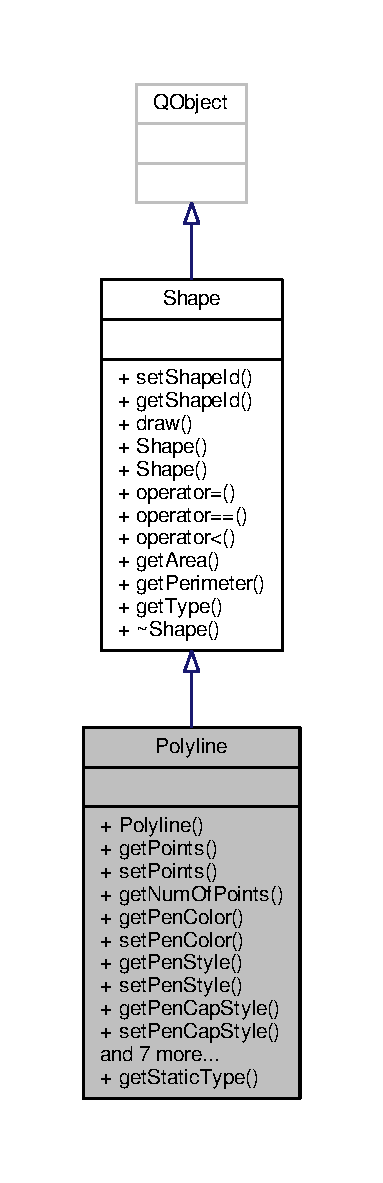
\includegraphics[height=550pt]{classPolyline__inherit__graph}
\end{center}
\end{figure}


Collaboration diagram for Polyline\+:\nopagebreak
\begin{figure}[H]
\begin{center}
\leavevmode
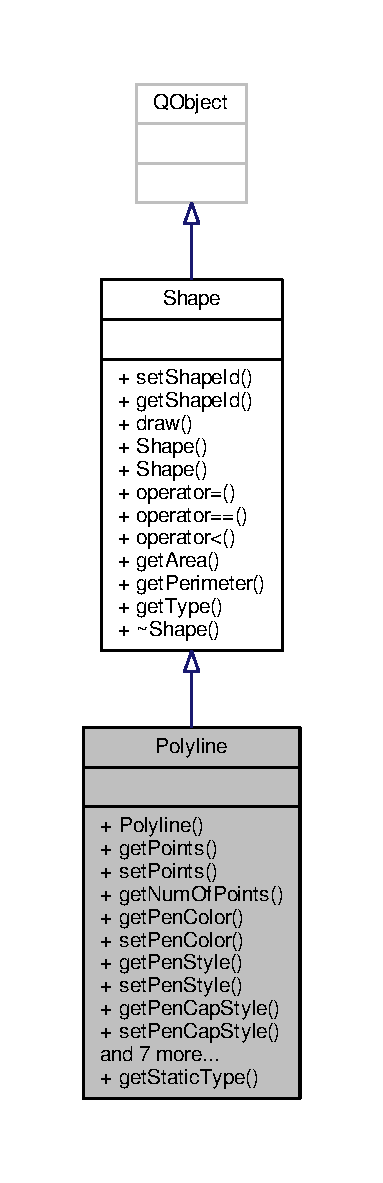
\includegraphics[height=550pt]{classPolyline__coll__graph}
\end{center}
\end{figure}
\subsection*{Public Member Functions}
\begin{DoxyCompactItemize}
\item 
\hyperlink{classPolyline_aaea9368c2e2bfc26ecaa36c7e125ac5e}{Polyline} (unsigned int, \hyperlink{classmyStd_1_1vector}{my\+Std\+::vector}$<$ Q\+Point $>$ \&, Qt\+::\+Global\+Color, Qt\+::\+Pen\+Style, \hyperlink{shape__input__file__specs_8txt_a622efdcfef6789d4367974d2fe79019e}{Qt\+::\+Pen\+Cap\+Style}, \hyperlink{shape__input__file__specs_8txt_a007db2043c6063881de2043c05c9c4a9}{Qt\+::\+Pen\+Join\+Style}, int)
\begin{DoxyCompactList}\small\item\em All parameter constructor. \end{DoxyCompactList}\item 
\hyperlink{classmyStd_1_1vector}{my\+Std\+::vector}$<$ Q\+Point $>$ \& \hyperlink{classPolyline_ae38a1e1f4d3a0506cac0afcee0cbf93e}{get\+Points} ()
\begin{DoxyCompactList}\small\item\em Gets the vector of Q\+Points that make up the polyline. \end{DoxyCompactList}\item 
void \hyperlink{classPolyline_a39d80ee69de06bb2037e6d73a21643b3}{set\+Points} (const \hyperlink{classmyStd_1_1vector}{my\+Std\+::vector}$<$ Q\+Point $>$ \&pts)
\begin{DoxyCompactList}\small\item\em Sets the vector of Q\+Points that make up the polyline to the given vector of Q\+Points. \end{DoxyCompactList}\item 
int \hyperlink{classPolyline_ac81ab6c46f172b381cc7b6ed4d6ec942}{get\+Num\+Of\+Points} ()
\begin{DoxyCompactList}\small\item\em Gets the number of points that make up the polyline. \end{DoxyCompactList}\item 
Qt\+::\+Global\+Color \hyperlink{classPolyline_a334e86d5b90a0f90649c64d37e95cff9}{get\+Pen\+Color} ()
\begin{DoxyCompactList}\small\item\em Gets the pen color stored in this shape. \end{DoxyCompactList}\item 
void \hyperlink{classPolyline_a69a07839c0f7c67efe10701bd7d7cf8e}{set\+Pen\+Color} (Qt\+::\+Global\+Color pc)
\begin{DoxyCompactList}\small\item\em Sets the color of the pen to the given color. \end{DoxyCompactList}\item 
Qt\+::\+Pen\+Style \hyperlink{classPolyline_aefe298425b83dbc94724ab5cb215bba3}{get\+Pen\+Style} ()
\begin{DoxyCompactList}\small\item\em Gets the style of the pen stored in the shape. \end{DoxyCompactList}\item 
void \hyperlink{classPolyline_ae5af058a4a94979fa88c2c3267da9087}{set\+Pen\+Style} (Qt\+::\+Pen\+Style ps)
\begin{DoxyCompactList}\small\item\em Sets the style of the pen to the given style. \end{DoxyCompactList}\item 
\hyperlink{shape__input__file__specs_8txt_a622efdcfef6789d4367974d2fe79019e}{Qt\+::\+Pen\+Cap\+Style} \hyperlink{classPolyline_acd78e365c667da035656279076bf5fe1}{get\+Pen\+Cap\+Style} ()
\begin{DoxyCompactList}\small\item\em Gets the pen cap style that is stored in this \hyperlink{classShape}{Shape}. \end{DoxyCompactList}\item 
void \hyperlink{classPolyline_a34510d4e398ec607c0ec125f380f30ff}{set\+Pen\+Cap\+Style} (\hyperlink{shape__input__file__specs_8txt_a622efdcfef6789d4367974d2fe79019e}{Qt\+::\+Pen\+Cap\+Style} pcs)
\begin{DoxyCompactList}\small\item\em Sets the Pen Cap Style to the given Pen Cap Style. \end{DoxyCompactList}\item 
\hyperlink{shape__input__file__specs_8txt_a007db2043c6063881de2043c05c9c4a9}{Qt\+::\+Pen\+Join\+Style} \hyperlink{classPolyline_a6bd520d9c7fef132bc43cbf61168917c}{get\+Pen\+Join\+Style} ()
\begin{DoxyCompactList}\small\item\em Gets the Pen Join Style. \end{DoxyCompactList}\item 
void \hyperlink{classPolyline_a3e792c8055d6c064afd6d6d07c7d8843}{set\+Pen\+Join\+Style} (\hyperlink{shape__input__file__specs_8txt_a007db2043c6063881de2043c05c9c4a9}{Qt\+::\+Pen\+Join\+Style} pjs)
\begin{DoxyCompactList}\small\item\em Sets the pen join style to the given style. \end{DoxyCompactList}\item 
int \hyperlink{classPolyline_ab01dd06f45e43dc9e6617596065fee70}{get\+Pen\+Width} ()
\begin{DoxyCompactList}\small\item\em Gets the width of the pen. \end{DoxyCompactList}\item 
void \hyperlink{classPolyline_aeb5424c425e44adff787367a497fc024}{set\+Pen\+Width} (int pw)
\begin{DoxyCompactList}\small\item\em Sets the width of the pen to the given width. \end{DoxyCompactList}\item 
virtual void \hyperlink{classPolyline_ac5b5a4ac26b140a7dc30cc293638e3ee}{draw} (Q\+Painter \&, bool)
\begin{DoxyCompactList}\small\item\em Virtual function to draw shapes. \end{DoxyCompactList}\item 
virtual int \hyperlink{classPolyline_a6138f6313141e81d989622806476c3d2}{get\+Type} ()
\begin{DoxyCompactList}\small\item\em Gets the type of the shape. \end{DoxyCompactList}\item 
virtual double \hyperlink{classPolyline_ad5425297b32d53a0f74eda253d4540f7}{get\+Perimeter} ()
\begin{DoxyCompactList}\small\item\em Gets the perimeter of the given shape. \end{DoxyCompactList}\end{DoxyCompactItemize}
\subsection*{Static Public Member Functions}
\begin{DoxyCompactItemize}
\item 
static int \hyperlink{classPolyline_abe58d8a06186437737d4c2f856328855}{get\+Static\+Type} ()
\begin{DoxyCompactList}\small\item\em gets the Type of object \end{DoxyCompactList}\end{DoxyCompactItemize}


\subsection{Detailed Description}
\hyperlink{classPolyline}{Polyline} class that Q\+Painter can draw. 

\subsection{Constructor \& Destructor Documentation}
\index{Polyline@{Polyline}!Polyline@{Polyline}}
\index{Polyline@{Polyline}!Polyline@{Polyline}}
\subsubsection[{\texorpdfstring{Polyline(unsigned int, my\+Std\+::vector$<$ Q\+Point $>$ \&, Qt\+::\+Global\+Color, Qt\+::\+Pen\+Style, Qt\+::\+Pen\+Cap\+Style, Qt\+::\+Pen\+Join\+Style, int)}{Polyline(unsigned int, myStd::vector< QPoint > &, Qt::GlobalColor, Qt::PenStyle, Qt::PenCapStyle, Qt::PenJoinStyle, int)}}]{\setlength{\rightskip}{0pt plus 5cm}Polyline\+::\+Polyline (
\begin{DoxyParamCaption}
\item[{unsigned int}]{i, }
\item[{{\bf my\+Std\+::vector}$<$ Q\+Point $>$ \&}]{vec, }
\item[{Qt\+::\+Global\+Color}]{pc, }
\item[{Qt\+::\+Pen\+Style}]{ps, }
\item[{{\bf Qt\+::\+Pen\+Cap\+Style}}]{pcs, }
\item[{{\bf Qt\+::\+Pen\+Join\+Style}}]{pjs, }
\item[{int}]{pw}
\end{DoxyParamCaption}
)}\hypertarget{classPolyline_aaea9368c2e2bfc26ecaa36c7e125ac5e}{}\label{classPolyline_aaea9368c2e2bfc26ecaa36c7e125ac5e}


All parameter constructor. 



\subsection{Member Function Documentation}
\index{Polyline@{Polyline}!draw@{draw}}
\index{draw@{draw}!Polyline@{Polyline}}
\subsubsection[{\texorpdfstring{draw(\+Q\+Painter \&, bool)}{draw(QPainter &, bool)}}]{\setlength{\rightskip}{0pt plus 5cm}void Polyline\+::draw (
\begin{DoxyParamCaption}
\item[{Q\+Painter \&}]{, }
\item[{bool}]{}
\end{DoxyParamCaption}
)\hspace{0.3cm}{\ttfamily [virtual]}}\hypertarget{classPolyline_ac5b5a4ac26b140a7dc30cc293638e3ee}{}\label{classPolyline_ac5b5a4ac26b140a7dc30cc293638e3ee}


Virtual function to draw shapes. 



Implements \hyperlink{classShape_a47dae32819e64fb32f3357f31978293f}{Shape}.

\index{Polyline@{Polyline}!get\+Num\+Of\+Points@{get\+Num\+Of\+Points}}
\index{get\+Num\+Of\+Points@{get\+Num\+Of\+Points}!Polyline@{Polyline}}
\subsubsection[{\texorpdfstring{get\+Num\+Of\+Points()}{getNumOfPoints()}}]{\setlength{\rightskip}{0pt plus 5cm}int Polyline\+::get\+Num\+Of\+Points (
\begin{DoxyParamCaption}
{}
\end{DoxyParamCaption}
)\hspace{0.3cm}{\ttfamily [inline]}}\hypertarget{classPolyline_ac81ab6c46f172b381cc7b6ed4d6ec942}{}\label{classPolyline_ac81ab6c46f172b381cc7b6ed4d6ec942}


Gets the number of points that make up the polyline. 

\begin{DoxyReturn}{Returns}
int number of Q\+Points 
\end{DoxyReturn}
\index{Polyline@{Polyline}!get\+Pen\+Cap\+Style@{get\+Pen\+Cap\+Style}}
\index{get\+Pen\+Cap\+Style@{get\+Pen\+Cap\+Style}!Polyline@{Polyline}}
\subsubsection[{\texorpdfstring{get\+Pen\+Cap\+Style()}{getPenCapStyle()}}]{\setlength{\rightskip}{0pt plus 5cm}{\bf Qt\+::\+Pen\+Cap\+Style} Polyline\+::get\+Pen\+Cap\+Style (
\begin{DoxyParamCaption}
{}
\end{DoxyParamCaption}
)\hspace{0.3cm}{\ttfamily [inline]}}\hypertarget{classPolyline_acd78e365c667da035656279076bf5fe1}{}\label{classPolyline_acd78e365c667da035656279076bf5fe1}


Gets the pen cap style that is stored in this \hyperlink{classShape}{Shape}. 

\begin{DoxyReturn}{Returns}
Pen\+Cap\+Style 
\end{DoxyReturn}
\index{Polyline@{Polyline}!get\+Pen\+Color@{get\+Pen\+Color}}
\index{get\+Pen\+Color@{get\+Pen\+Color}!Polyline@{Polyline}}
\subsubsection[{\texorpdfstring{get\+Pen\+Color()}{getPenColor()}}]{\setlength{\rightskip}{0pt plus 5cm}Qt\+::\+Global\+Color Polyline\+::get\+Pen\+Color (
\begin{DoxyParamCaption}
{}
\end{DoxyParamCaption}
)\hspace{0.3cm}{\ttfamily [inline]}}\hypertarget{classPolyline_a334e86d5b90a0f90649c64d37e95cff9}{}\label{classPolyline_a334e86d5b90a0f90649c64d37e95cff9}


Gets the pen color stored in this shape. 

\begin{DoxyReturn}{Returns}
Color of the pen 
\end{DoxyReturn}
\index{Polyline@{Polyline}!get\+Pen\+Join\+Style@{get\+Pen\+Join\+Style}}
\index{get\+Pen\+Join\+Style@{get\+Pen\+Join\+Style}!Polyline@{Polyline}}
\subsubsection[{\texorpdfstring{get\+Pen\+Join\+Style()}{getPenJoinStyle()}}]{\setlength{\rightskip}{0pt plus 5cm}{\bf Qt\+::\+Pen\+Join\+Style} Polyline\+::get\+Pen\+Join\+Style (
\begin{DoxyParamCaption}
{}
\end{DoxyParamCaption}
)\hspace{0.3cm}{\ttfamily [inline]}}\hypertarget{classPolyline_a6bd520d9c7fef132bc43cbf61168917c}{}\label{classPolyline_a6bd520d9c7fef132bc43cbf61168917c}


Gets the Pen Join Style. 

\begin{DoxyReturn}{Returns}
Pen\+Join\+Style 
\end{DoxyReturn}
\index{Polyline@{Polyline}!get\+Pen\+Style@{get\+Pen\+Style}}
\index{get\+Pen\+Style@{get\+Pen\+Style}!Polyline@{Polyline}}
\subsubsection[{\texorpdfstring{get\+Pen\+Style()}{getPenStyle()}}]{\setlength{\rightskip}{0pt plus 5cm}Qt\+::\+Pen\+Style Polyline\+::get\+Pen\+Style (
\begin{DoxyParamCaption}
{}
\end{DoxyParamCaption}
)\hspace{0.3cm}{\ttfamily [inline]}}\hypertarget{classPolyline_aefe298425b83dbc94724ab5cb215bba3}{}\label{classPolyline_aefe298425b83dbc94724ab5cb215bba3}


Gets the style of the pen stored in the shape. 

\begin{DoxyReturn}{Returns}
Style of the pen 
\end{DoxyReturn}
\index{Polyline@{Polyline}!get\+Pen\+Width@{get\+Pen\+Width}}
\index{get\+Pen\+Width@{get\+Pen\+Width}!Polyline@{Polyline}}
\subsubsection[{\texorpdfstring{get\+Pen\+Width()}{getPenWidth()}}]{\setlength{\rightskip}{0pt plus 5cm}int Polyline\+::get\+Pen\+Width (
\begin{DoxyParamCaption}
{}
\end{DoxyParamCaption}
)\hspace{0.3cm}{\ttfamily [inline]}}\hypertarget{classPolyline_ab01dd06f45e43dc9e6617596065fee70}{}\label{classPolyline_ab01dd06f45e43dc9e6617596065fee70}


Gets the width of the pen. 

\begin{DoxyReturn}{Returns}
pen\+Width 
\end{DoxyReturn}
\index{Polyline@{Polyline}!get\+Perimeter@{get\+Perimeter}}
\index{get\+Perimeter@{get\+Perimeter}!Polyline@{Polyline}}
\subsubsection[{\texorpdfstring{get\+Perimeter()}{getPerimeter()}}]{\setlength{\rightskip}{0pt plus 5cm}virtual double Polyline\+::get\+Perimeter (
\begin{DoxyParamCaption}
{}
\end{DoxyParamCaption}
)\hspace{0.3cm}{\ttfamily [inline]}, {\ttfamily [virtual]}}\hypertarget{classPolyline_ad5425297b32d53a0f74eda253d4540f7}{}\label{classPolyline_ad5425297b32d53a0f74eda253d4540f7}


Gets the perimeter of the given shape. 

\begin{DoxyReturn}{Returns}
Perimeter as a double 
\end{DoxyReturn}


Reimplemented from \hyperlink{classShape_a391744b6bce96df044139dcbd1ae0aa8}{Shape}.

\index{Polyline@{Polyline}!get\+Points@{get\+Points}}
\index{get\+Points@{get\+Points}!Polyline@{Polyline}}
\subsubsection[{\texorpdfstring{get\+Points()}{getPoints()}}]{\setlength{\rightskip}{0pt plus 5cm}{\bf my\+Std\+::vector}$<$Q\+Point$>$\& Polyline\+::get\+Points (
\begin{DoxyParamCaption}
{}
\end{DoxyParamCaption}
)\hspace{0.3cm}{\ttfamily [inline]}}\hypertarget{classPolyline_ae38a1e1f4d3a0506cac0afcee0cbf93e}{}\label{classPolyline_ae38a1e1f4d3a0506cac0afcee0cbf93e}


Gets the vector of Q\+Points that make up the polyline. 

\begin{DoxyReturn}{Returns}
vector of Q\+Points 
\end{DoxyReturn}
\index{Polyline@{Polyline}!get\+Static\+Type@{get\+Static\+Type}}
\index{get\+Static\+Type@{get\+Static\+Type}!Polyline@{Polyline}}
\subsubsection[{\texorpdfstring{get\+Static\+Type()}{getStaticType()}}]{\setlength{\rightskip}{0pt plus 5cm}static int Polyline\+::get\+Static\+Type (
\begin{DoxyParamCaption}
{}
\end{DoxyParamCaption}
)\hspace{0.3cm}{\ttfamily [inline]}, {\ttfamily [static]}}\hypertarget{classPolyline_abe58d8a06186437737d4c2f856328855}{}\label{classPolyline_abe58d8a06186437737d4c2f856328855}


gets the Type of object 

\begin{DoxyReturn}{Returns}
Type as int 
\end{DoxyReturn}
\index{Polyline@{Polyline}!get\+Type@{get\+Type}}
\index{get\+Type@{get\+Type}!Polyline@{Polyline}}
\subsubsection[{\texorpdfstring{get\+Type()}{getType()}}]{\setlength{\rightskip}{0pt plus 5cm}virtual int Polyline\+::get\+Type (
\begin{DoxyParamCaption}
{}
\end{DoxyParamCaption}
)\hspace{0.3cm}{\ttfamily [inline]}, {\ttfamily [virtual]}}\hypertarget{classPolyline_a6138f6313141e81d989622806476c3d2}{}\label{classPolyline_a6138f6313141e81d989622806476c3d2}


Gets the type of the shape. 

\begin{DoxyReturn}{Returns}
type as an int 
\end{DoxyReturn}


Implements \hyperlink{classShape_a3d15adf2a1d746928f9be98105096eda}{Shape}.

\index{Polyline@{Polyline}!set\+Pen\+Cap\+Style@{set\+Pen\+Cap\+Style}}
\index{set\+Pen\+Cap\+Style@{set\+Pen\+Cap\+Style}!Polyline@{Polyline}}
\subsubsection[{\texorpdfstring{set\+Pen\+Cap\+Style(\+Qt\+::\+Pen\+Cap\+Style pcs)}{setPenCapStyle(Qt::PenCapStyle pcs)}}]{\setlength{\rightskip}{0pt plus 5cm}void Polyline\+::set\+Pen\+Cap\+Style (
\begin{DoxyParamCaption}
\item[{{\bf Qt\+::\+Pen\+Cap\+Style}}]{pcs}
\end{DoxyParamCaption}
)\hspace{0.3cm}{\ttfamily [inline]}}\hypertarget{classPolyline_a34510d4e398ec607c0ec125f380f30ff}{}\label{classPolyline_a34510d4e398ec607c0ec125f380f30ff}


Sets the Pen Cap Style to the given Pen Cap Style. 


\begin{DoxyParams}{Parameters}
{\em pen\+Cap\+Style} & \\
\hline
\end{DoxyParams}
\index{Polyline@{Polyline}!set\+Pen\+Color@{set\+Pen\+Color}}
\index{set\+Pen\+Color@{set\+Pen\+Color}!Polyline@{Polyline}}
\subsubsection[{\texorpdfstring{set\+Pen\+Color(\+Qt\+::\+Global\+Color pc)}{setPenColor(Qt::GlobalColor pc)}}]{\setlength{\rightskip}{0pt plus 5cm}void Polyline\+::set\+Pen\+Color (
\begin{DoxyParamCaption}
\item[{Qt\+::\+Global\+Color}]{pc}
\end{DoxyParamCaption}
)\hspace{0.3cm}{\ttfamily [inline]}}\hypertarget{classPolyline_a69a07839c0f7c67efe10701bd7d7cf8e}{}\label{classPolyline_a69a07839c0f7c67efe10701bd7d7cf8e}


Sets the color of the pen to the given color. 


\begin{DoxyParams}{Parameters}
{\em pen\+Color} & \\
\hline
\end{DoxyParams}
\index{Polyline@{Polyline}!set\+Pen\+Join\+Style@{set\+Pen\+Join\+Style}}
\index{set\+Pen\+Join\+Style@{set\+Pen\+Join\+Style}!Polyline@{Polyline}}
\subsubsection[{\texorpdfstring{set\+Pen\+Join\+Style(\+Qt\+::\+Pen\+Join\+Style pjs)}{setPenJoinStyle(Qt::PenJoinStyle pjs)}}]{\setlength{\rightskip}{0pt plus 5cm}void Polyline\+::set\+Pen\+Join\+Style (
\begin{DoxyParamCaption}
\item[{{\bf Qt\+::\+Pen\+Join\+Style}}]{pjs}
\end{DoxyParamCaption}
)\hspace{0.3cm}{\ttfamily [inline]}}\hypertarget{classPolyline_a3e792c8055d6c064afd6d6d07c7d8843}{}\label{classPolyline_a3e792c8055d6c064afd6d6d07c7d8843}


Sets the pen join style to the given style. 


\begin{DoxyParams}{Parameters}
{\em pen\+Join\+Style} & \\
\hline
\end{DoxyParams}
\index{Polyline@{Polyline}!set\+Pen\+Style@{set\+Pen\+Style}}
\index{set\+Pen\+Style@{set\+Pen\+Style}!Polyline@{Polyline}}
\subsubsection[{\texorpdfstring{set\+Pen\+Style(\+Qt\+::\+Pen\+Style ps)}{setPenStyle(Qt::PenStyle ps)}}]{\setlength{\rightskip}{0pt plus 5cm}void Polyline\+::set\+Pen\+Style (
\begin{DoxyParamCaption}
\item[{Qt\+::\+Pen\+Style}]{ps}
\end{DoxyParamCaption}
)\hspace{0.3cm}{\ttfamily [inline]}}\hypertarget{classPolyline_ae5af058a4a94979fa88c2c3267da9087}{}\label{classPolyline_ae5af058a4a94979fa88c2c3267da9087}


Sets the style of the pen to the given style. 


\begin{DoxyParams}{Parameters}
{\em pen\+Style} & \\
\hline
\end{DoxyParams}
\index{Polyline@{Polyline}!set\+Pen\+Width@{set\+Pen\+Width}}
\index{set\+Pen\+Width@{set\+Pen\+Width}!Polyline@{Polyline}}
\subsubsection[{\texorpdfstring{set\+Pen\+Width(int pw)}{setPenWidth(int pw)}}]{\setlength{\rightskip}{0pt plus 5cm}void Polyline\+::set\+Pen\+Width (
\begin{DoxyParamCaption}
\item[{int}]{pw}
\end{DoxyParamCaption}
)\hspace{0.3cm}{\ttfamily [inline]}}\hypertarget{classPolyline_aeb5424c425e44adff787367a497fc024}{}\label{classPolyline_aeb5424c425e44adff787367a497fc024}


Sets the width of the pen to the given width. 


\begin{DoxyParams}{Parameters}
{\em pen\+Width} & \\
\hline
\end{DoxyParams}
\index{Polyline@{Polyline}!set\+Points@{set\+Points}}
\index{set\+Points@{set\+Points}!Polyline@{Polyline}}
\subsubsection[{\texorpdfstring{set\+Points(const my\+Std\+::vector$<$ Q\+Point $>$ \&pts)}{setPoints(const myStd::vector< QPoint > &pts)}}]{\setlength{\rightskip}{0pt plus 5cm}void Polyline\+::set\+Points (
\begin{DoxyParamCaption}
\item[{const {\bf my\+Std\+::vector}$<$ Q\+Point $>$ \&}]{pts}
\end{DoxyParamCaption}
)\hspace{0.3cm}{\ttfamily [inline]}}\hypertarget{classPolyline_a39d80ee69de06bb2037e6d73a21643b3}{}\label{classPolyline_a39d80ee69de06bb2037e6d73a21643b3}


Sets the vector of Q\+Points that make up the polyline to the given vector of Q\+Points. 


\begin{DoxyParams}{Parameters}
{\em pts} & vector of Q\+Points \\
\hline
\end{DoxyParams}


The documentation for this class was generated from the following files\+:\begin{DoxyCompactItemize}
\item 
Group Project/\+Scrum\+Of\+The\+Earth/\hyperlink{polyline_8h}{polyline.\+h}\item 
Group Project/\+Scrum\+Of\+The\+Earth/\hyperlink{polyline_8cpp}{polyline.\+cpp}\end{DoxyCompactItemize}

\hypertarget{classRectangle}{}\section{Rectangle Class Reference}
\label{classRectangle}\index{Rectangle@{Rectangle}}


\hyperlink{classRectangle}{Rectangle} class that Q\+Painter can draw.  




{\ttfamily \#include $<$rectangle.\+h$>$}



Inheritance diagram for Rectangle\+:\nopagebreak
\begin{figure}[H]
\begin{center}
\leavevmode
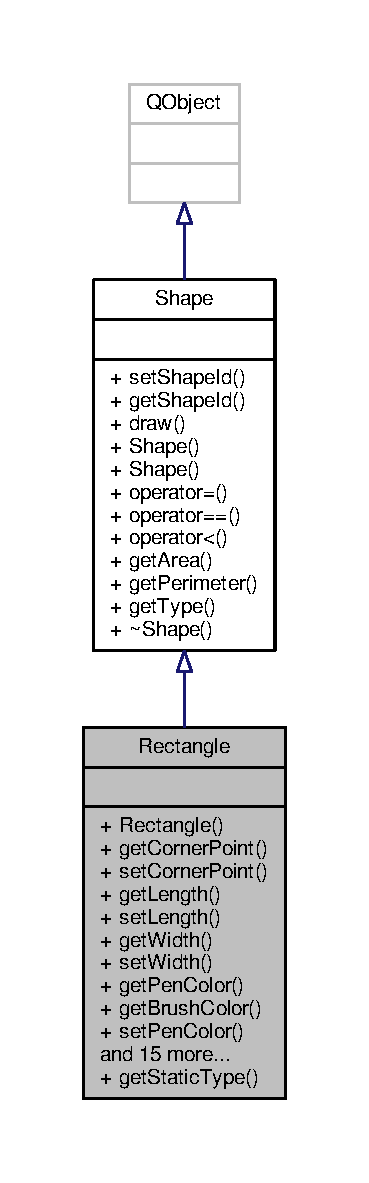
\includegraphics[height=550pt]{classRectangle__inherit__graph}
\end{center}
\end{figure}


Collaboration diagram for Rectangle\+:\nopagebreak
\begin{figure}[H]
\begin{center}
\leavevmode
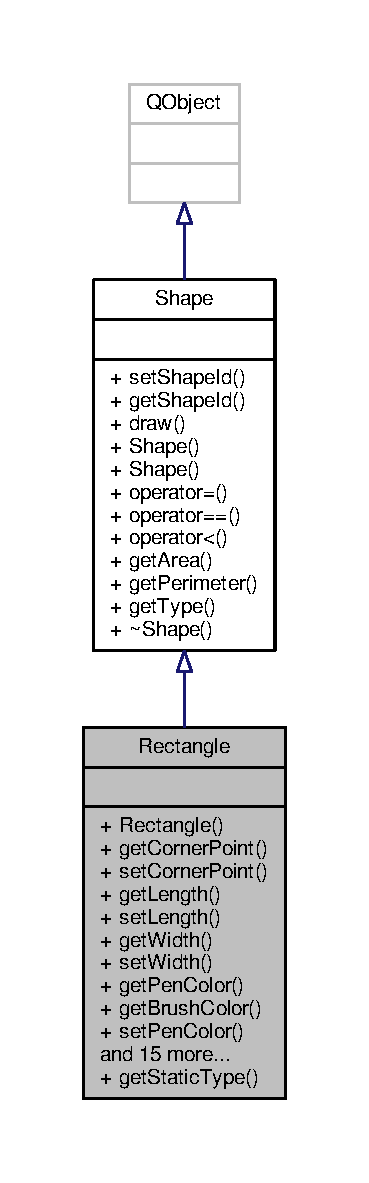
\includegraphics[height=550pt]{classRectangle__coll__graph}
\end{center}
\end{figure}
\subsection*{Public Member Functions}
\begin{DoxyCompactItemize}
\item 
\hyperlink{classRectangle_a1dca3e66dc1317df74dda6c1984728ff}{Rectangle} (unsigned int, int, int, int, int, Qt\+::\+Global\+Color, Qt\+::\+Global\+Color, Qt\+::\+Pen\+Style, \hyperlink{shape__input__file__specs_8txt_a622efdcfef6789d4367974d2fe79019e}{Qt\+::\+Pen\+Cap\+Style}, \hyperlink{shape__input__file__specs_8txt_a007db2043c6063881de2043c05c9c4a9}{Qt\+::\+Pen\+Join\+Style}, \hyperlink{shape__input__file__specs_8txt_ad07f6fe6c28dcb0b3bdc324a72d0051f}{Qt\+::\+Brush\+Style}, int)
\begin{DoxyCompactList}\small\item\em All parameter constructor. \end{DoxyCompactList}\item 
Q\+Point \hyperlink{classRectangle_a934ec26d7cff08b196e6e2db94508d5d}{get\+Corner\+Point} ()
\begin{DoxyCompactList}\small\item\em Gets the top left corner point of the rectangle. \end{DoxyCompactList}\item 
void \hyperlink{classRectangle_a34488ca08ac813751dba8c57c80985fa}{set\+Corner\+Point} (Q\+Point p1)
\begin{DoxyCompactList}\small\item\em Sets the top left corner point to the given point. \end{DoxyCompactList}\item 
int \hyperlink{classRectangle_a58c26a2910e8982b49fafd02d1d3aa47}{get\+Length} ()
\begin{DoxyCompactList}\small\item\em Gets the length of the rectangle. \end{DoxyCompactList}\item 
void \hyperlink{classRectangle_a8186780b0db41885ed04c45c9caafe96}{set\+Length} (int \hyperlink{shape__input__file__specs_8txt_a2e02238fe11bc76d2a69c565c7391545}{l})
\begin{DoxyCompactList}\small\item\em Sets the length of the rectangle to the given length. \end{DoxyCompactList}\item 
int \hyperlink{classRectangle_ab750e4f0666df9c303ad649342bf3efd}{get\+Width} ()
\begin{DoxyCompactList}\small\item\em Gets the width of the rectangle. \end{DoxyCompactList}\item 
void \hyperlink{classRectangle_a4b2a528eff1c42b1a46148b2f5562c7b}{set\+Width} (int w)
\begin{DoxyCompactList}\small\item\em Sets the width of the rectangle. \end{DoxyCompactList}\item 
Qt\+::\+Global\+Color \hyperlink{classRectangle_a260ef02e14a452e25b1ebddc805928c8}{get\+Pen\+Color} ()
\begin{DoxyCompactList}\small\item\em Gets the pen color stored in this shape. \end{DoxyCompactList}\item 
Qt\+::\+Global\+Color \hyperlink{classRectangle_af105857f6e7bda45c45d0ce1309a032e}{get\+Brush\+Color} ()
\begin{DoxyCompactList}\small\item\em Gets the Brush color stored in the \hyperlink{classShape}{Shape}. \end{DoxyCompactList}\item 
void \hyperlink{classRectangle_a489b9d60a05a4d2f6ee01d7989b30c22}{set\+Pen\+Color} (Qt\+::\+Global\+Color pc)
\begin{DoxyCompactList}\small\item\em Sets the color of the pen to the given color. \end{DoxyCompactList}\item 
void \hyperlink{classRectangle_a645117a96beb4782f2ffc00d0ab865e1}{set\+Brush\+Color} (Qt\+::\+Global\+Color bc)
\begin{DoxyCompactList}\small\item\em Sets the color of the Brush to the given color. \end{DoxyCompactList}\item 
Qt\+::\+Pen\+Style \hyperlink{classRectangle_abb61dc270e5b2b4ae3323e097e6fb7ce}{get\+Pen\+Style} ()
\begin{DoxyCompactList}\small\item\em Gets the style of the pen stored in the shape. \end{DoxyCompactList}\item 
void \hyperlink{classRectangle_a598da91b42f1f3541f687d6c35c23d23}{set\+Pen\+Style} (Qt\+::\+Pen\+Style ps)
\begin{DoxyCompactList}\small\item\em Sets the style of the pen to the given style. \end{DoxyCompactList}\item 
\hyperlink{shape__input__file__specs_8txt_a622efdcfef6789d4367974d2fe79019e}{Qt\+::\+Pen\+Cap\+Style} \hyperlink{classRectangle_a7e42f496cbaa93545c370a1a4aef4d42}{get\+Pen\+Cap\+Style} ()
\begin{DoxyCompactList}\small\item\em Gets the pen cap style that is stored in this \hyperlink{classShape}{Shape}. \end{DoxyCompactList}\item 
void \hyperlink{classRectangle_a18f32cd496f2298ca9165231943c3bae}{set\+Pen\+Cap\+Style} (\hyperlink{shape__input__file__specs_8txt_a622efdcfef6789d4367974d2fe79019e}{Qt\+::\+Pen\+Cap\+Style} pcs)
\begin{DoxyCompactList}\small\item\em Sets the Pen Cap Style to the given Pen Cap Style. \end{DoxyCompactList}\item 
\hyperlink{shape__input__file__specs_8txt_a007db2043c6063881de2043c05c9c4a9}{Qt\+::\+Pen\+Join\+Style} \hyperlink{classRectangle_aaeb26e28ee7b37e166caeb1bf4ea7ec4}{get\+Pen\+Join\+Style} ()
\begin{DoxyCompactList}\small\item\em Gets the Pen Join Style. \end{DoxyCompactList}\item 
void \hyperlink{classRectangle_acdb9bcb2c87a84c84b33a4a99c239de6}{set\+Pen\+Join\+Style} (\hyperlink{shape__input__file__specs_8txt_a007db2043c6063881de2043c05c9c4a9}{Qt\+::\+Pen\+Join\+Style} pjs)
\begin{DoxyCompactList}\small\item\em Sets the pen join style to the given style. \end{DoxyCompactList}\item 
\hyperlink{shape__input__file__specs_8txt_ad07f6fe6c28dcb0b3bdc324a72d0051f}{Qt\+::\+Brush\+Style} \hyperlink{classRectangle_aaa486dcefcdd7e59e63d92c105876724}{get\+Brush\+Style} ()
\begin{DoxyCompactList}\small\item\em Gets the Brush Style. \end{DoxyCompactList}\item 
void \hyperlink{classRectangle_a4d5dff9ac01e605872f80d110015041b}{set\+Brush\+Style} (\hyperlink{shape__input__file__specs_8txt_ad07f6fe6c28dcb0b3bdc324a72d0051f}{Qt\+::\+Brush\+Style} bs)
\begin{DoxyCompactList}\small\item\em Sets the Brush Style to the given Brush Style. \end{DoxyCompactList}\item 
int \hyperlink{classRectangle_a45243b7fbe88527e6aed399b37863305}{get\+Pen\+Width} ()
\begin{DoxyCompactList}\small\item\em Gets the width of the pen. \end{DoxyCompactList}\item 
void \hyperlink{classRectangle_aa4e06745d54628776b1ac0f85c1e9867}{set\+Pen\+Width} (int pw)
\begin{DoxyCompactList}\small\item\em Sets the width of the pen to the given width. \end{DoxyCompactList}\item 
virtual void \hyperlink{classRectangle_a6734cad19e207a212dcb042e1006a7f1}{draw} (Q\+Painter \&, bool)
\begin{DoxyCompactList}\small\item\em Virtual function to draw shapes. \end{DoxyCompactList}\item 
virtual int \hyperlink{classRectangle_a0098e1642c4ff1180c1243b802caca5a}{get\+Type} ()
\begin{DoxyCompactList}\small\item\em Gets the type of the shape. \end{DoxyCompactList}\item 
virtual double \hyperlink{classRectangle_a5405044e619a5ba1a52c0b9607c9f166}{get\+Area} ()
\begin{DoxyCompactList}\small\item\em Gets the area of the given shape. \end{DoxyCompactList}\item 
virtual double \hyperlink{classRectangle_aba6936b3c376465edff938cd4affc914}{get\+Perimeter} ()
\begin{DoxyCompactList}\small\item\em Gets the perimeter of the given shape. \end{DoxyCompactList}\end{DoxyCompactItemize}
\subsection*{Static Public Member Functions}
\begin{DoxyCompactItemize}
\item 
static int \hyperlink{classRectangle_ac9e18cf57224bfbc584547c0ee6d1ce3}{get\+Static\+Type} ()
\begin{DoxyCompactList}\small\item\em gets the Type of object \end{DoxyCompactList}\end{DoxyCompactItemize}


\subsection{Detailed Description}
\hyperlink{classRectangle}{Rectangle} class that Q\+Painter can draw. 

\subsection{Constructor \& Destructor Documentation}
\index{Rectangle@{Rectangle}!Rectangle@{Rectangle}}
\index{Rectangle@{Rectangle}!Rectangle@{Rectangle}}
\subsubsection[{\texorpdfstring{Rectangle(unsigned int, int, int, int, int, Qt\+::\+Global\+Color, Qt\+::\+Global\+Color, Qt\+::\+Pen\+Style, Qt\+::\+Pen\+Cap\+Style, Qt\+::\+Pen\+Join\+Style, Qt\+::\+Brush\+Style, int)}{Rectangle(unsigned int, int, int, int, int, Qt::GlobalColor, Qt::GlobalColor, Qt::PenStyle, Qt::PenCapStyle, Qt::PenJoinStyle, Qt::BrushStyle, int)}}]{\setlength{\rightskip}{0pt plus 5cm}Rectangle\+::\+Rectangle (
\begin{DoxyParamCaption}
\item[{unsigned int}]{i, }
\item[{int}]{x, }
\item[{int}]{y, }
\item[{int}]{l, }
\item[{int}]{w, }
\item[{Qt\+::\+Global\+Color}]{pc, }
\item[{Qt\+::\+Global\+Color}]{bc, }
\item[{Qt\+::\+Pen\+Style}]{ps, }
\item[{{\bf Qt\+::\+Pen\+Cap\+Style}}]{pcs, }
\item[{{\bf Qt\+::\+Pen\+Join\+Style}}]{pjs, }
\item[{{\bf Qt\+::\+Brush\+Style}}]{bs, }
\item[{int}]{pw}
\end{DoxyParamCaption}
)}\hypertarget{classRectangle_a1dca3e66dc1317df74dda6c1984728ff}{}\label{classRectangle_a1dca3e66dc1317df74dda6c1984728ff}


All parameter constructor. 



\subsection{Member Function Documentation}
\index{Rectangle@{Rectangle}!draw@{draw}}
\index{draw@{draw}!Rectangle@{Rectangle}}
\subsubsection[{\texorpdfstring{draw(\+Q\+Painter \&, bool)}{draw(QPainter &, bool)}}]{\setlength{\rightskip}{0pt plus 5cm}void Rectangle\+::draw (
\begin{DoxyParamCaption}
\item[{Q\+Painter \&}]{, }
\item[{bool}]{}
\end{DoxyParamCaption}
)\hspace{0.3cm}{\ttfamily [virtual]}}\hypertarget{classRectangle_a6734cad19e207a212dcb042e1006a7f1}{}\label{classRectangle_a6734cad19e207a212dcb042e1006a7f1}


Virtual function to draw shapes. 



Implements \hyperlink{classShape_a47dae32819e64fb32f3357f31978293f}{Shape}.

\index{Rectangle@{Rectangle}!get\+Area@{get\+Area}}
\index{get\+Area@{get\+Area}!Rectangle@{Rectangle}}
\subsubsection[{\texorpdfstring{get\+Area()}{getArea()}}]{\setlength{\rightskip}{0pt plus 5cm}virtual double Rectangle\+::get\+Area (
\begin{DoxyParamCaption}
{}
\end{DoxyParamCaption}
)\hspace{0.3cm}{\ttfamily [inline]}, {\ttfamily [virtual]}}\hypertarget{classRectangle_a5405044e619a5ba1a52c0b9607c9f166}{}\label{classRectangle_a5405044e619a5ba1a52c0b9607c9f166}


Gets the area of the given shape. 

\begin{DoxyReturn}{Returns}
Area as a double 
\end{DoxyReturn}


Reimplemented from \hyperlink{classShape_ac29f8bce0d038c84470028c6819a79ab}{Shape}.

\index{Rectangle@{Rectangle}!get\+Brush\+Color@{get\+Brush\+Color}}
\index{get\+Brush\+Color@{get\+Brush\+Color}!Rectangle@{Rectangle}}
\subsubsection[{\texorpdfstring{get\+Brush\+Color()}{getBrushColor()}}]{\setlength{\rightskip}{0pt plus 5cm}Qt\+::\+Global\+Color Rectangle\+::get\+Brush\+Color (
\begin{DoxyParamCaption}
{}
\end{DoxyParamCaption}
)\hspace{0.3cm}{\ttfamily [inline]}}\hypertarget{classRectangle_af105857f6e7bda45c45d0ce1309a032e}{}\label{classRectangle_af105857f6e7bda45c45d0ce1309a032e}


Gets the Brush color stored in the \hyperlink{classShape}{Shape}. 

\begin{DoxyReturn}{Returns}
Color of the Brush 
\end{DoxyReturn}
\index{Rectangle@{Rectangle}!get\+Brush\+Style@{get\+Brush\+Style}}
\index{get\+Brush\+Style@{get\+Brush\+Style}!Rectangle@{Rectangle}}
\subsubsection[{\texorpdfstring{get\+Brush\+Style()}{getBrushStyle()}}]{\setlength{\rightskip}{0pt plus 5cm}{\bf Qt\+::\+Brush\+Style} Rectangle\+::get\+Brush\+Style (
\begin{DoxyParamCaption}
{}
\end{DoxyParamCaption}
)\hspace{0.3cm}{\ttfamily [inline]}}\hypertarget{classRectangle_aaa486dcefcdd7e59e63d92c105876724}{}\label{classRectangle_aaa486dcefcdd7e59e63d92c105876724}


Gets the Brush Style. 

\begin{DoxyReturn}{Returns}
Brush\+Style 
\end{DoxyReturn}
\index{Rectangle@{Rectangle}!get\+Corner\+Point@{get\+Corner\+Point}}
\index{get\+Corner\+Point@{get\+Corner\+Point}!Rectangle@{Rectangle}}
\subsubsection[{\texorpdfstring{get\+Corner\+Point()}{getCornerPoint()}}]{\setlength{\rightskip}{0pt plus 5cm}Q\+Point Rectangle\+::get\+Corner\+Point (
\begin{DoxyParamCaption}
{}
\end{DoxyParamCaption}
)\hspace{0.3cm}{\ttfamily [inline]}}\hypertarget{classRectangle_a934ec26d7cff08b196e6e2db94508d5d}{}\label{classRectangle_a934ec26d7cff08b196e6e2db94508d5d}


Gets the top left corner point of the rectangle. 

\begin{DoxyReturn}{Returns}
Q\+Point of the top left point 
\end{DoxyReturn}
\index{Rectangle@{Rectangle}!get\+Length@{get\+Length}}
\index{get\+Length@{get\+Length}!Rectangle@{Rectangle}}
\subsubsection[{\texorpdfstring{get\+Length()}{getLength()}}]{\setlength{\rightskip}{0pt plus 5cm}int Rectangle\+::get\+Length (
\begin{DoxyParamCaption}
{}
\end{DoxyParamCaption}
)\hspace{0.3cm}{\ttfamily [inline]}}\hypertarget{classRectangle_a58c26a2910e8982b49fafd02d1d3aa47}{}\label{classRectangle_a58c26a2910e8982b49fafd02d1d3aa47}


Gets the length of the rectangle. 

\begin{DoxyReturn}{Returns}
int length of rectangle 
\end{DoxyReturn}
\index{Rectangle@{Rectangle}!get\+Pen\+Cap\+Style@{get\+Pen\+Cap\+Style}}
\index{get\+Pen\+Cap\+Style@{get\+Pen\+Cap\+Style}!Rectangle@{Rectangle}}
\subsubsection[{\texorpdfstring{get\+Pen\+Cap\+Style()}{getPenCapStyle()}}]{\setlength{\rightskip}{0pt plus 5cm}{\bf Qt\+::\+Pen\+Cap\+Style} Rectangle\+::get\+Pen\+Cap\+Style (
\begin{DoxyParamCaption}
{}
\end{DoxyParamCaption}
)\hspace{0.3cm}{\ttfamily [inline]}}\hypertarget{classRectangle_a7e42f496cbaa93545c370a1a4aef4d42}{}\label{classRectangle_a7e42f496cbaa93545c370a1a4aef4d42}


Gets the pen cap style that is stored in this \hyperlink{classShape}{Shape}. 

\begin{DoxyReturn}{Returns}
Pen\+Cap\+Style 
\end{DoxyReturn}
\index{Rectangle@{Rectangle}!get\+Pen\+Color@{get\+Pen\+Color}}
\index{get\+Pen\+Color@{get\+Pen\+Color}!Rectangle@{Rectangle}}
\subsubsection[{\texorpdfstring{get\+Pen\+Color()}{getPenColor()}}]{\setlength{\rightskip}{0pt plus 5cm}Qt\+::\+Global\+Color Rectangle\+::get\+Pen\+Color (
\begin{DoxyParamCaption}
{}
\end{DoxyParamCaption}
)\hspace{0.3cm}{\ttfamily [inline]}}\hypertarget{classRectangle_a260ef02e14a452e25b1ebddc805928c8}{}\label{classRectangle_a260ef02e14a452e25b1ebddc805928c8}


Gets the pen color stored in this shape. 

\begin{DoxyReturn}{Returns}
Color of the pen 
\end{DoxyReturn}
\index{Rectangle@{Rectangle}!get\+Pen\+Join\+Style@{get\+Pen\+Join\+Style}}
\index{get\+Pen\+Join\+Style@{get\+Pen\+Join\+Style}!Rectangle@{Rectangle}}
\subsubsection[{\texorpdfstring{get\+Pen\+Join\+Style()}{getPenJoinStyle()}}]{\setlength{\rightskip}{0pt plus 5cm}{\bf Qt\+::\+Pen\+Join\+Style} Rectangle\+::get\+Pen\+Join\+Style (
\begin{DoxyParamCaption}
{}
\end{DoxyParamCaption}
)\hspace{0.3cm}{\ttfamily [inline]}}\hypertarget{classRectangle_aaeb26e28ee7b37e166caeb1bf4ea7ec4}{}\label{classRectangle_aaeb26e28ee7b37e166caeb1bf4ea7ec4}


Gets the Pen Join Style. 

\begin{DoxyReturn}{Returns}
Pen\+Join\+Style 
\end{DoxyReturn}
\index{Rectangle@{Rectangle}!get\+Pen\+Style@{get\+Pen\+Style}}
\index{get\+Pen\+Style@{get\+Pen\+Style}!Rectangle@{Rectangle}}
\subsubsection[{\texorpdfstring{get\+Pen\+Style()}{getPenStyle()}}]{\setlength{\rightskip}{0pt plus 5cm}Qt\+::\+Pen\+Style Rectangle\+::get\+Pen\+Style (
\begin{DoxyParamCaption}
{}
\end{DoxyParamCaption}
)\hspace{0.3cm}{\ttfamily [inline]}}\hypertarget{classRectangle_abb61dc270e5b2b4ae3323e097e6fb7ce}{}\label{classRectangle_abb61dc270e5b2b4ae3323e097e6fb7ce}


Gets the style of the pen stored in the shape. 

\begin{DoxyReturn}{Returns}
Style of the pen 
\end{DoxyReturn}
\index{Rectangle@{Rectangle}!get\+Pen\+Width@{get\+Pen\+Width}}
\index{get\+Pen\+Width@{get\+Pen\+Width}!Rectangle@{Rectangle}}
\subsubsection[{\texorpdfstring{get\+Pen\+Width()}{getPenWidth()}}]{\setlength{\rightskip}{0pt plus 5cm}int Rectangle\+::get\+Pen\+Width (
\begin{DoxyParamCaption}
{}
\end{DoxyParamCaption}
)\hspace{0.3cm}{\ttfamily [inline]}}\hypertarget{classRectangle_a45243b7fbe88527e6aed399b37863305}{}\label{classRectangle_a45243b7fbe88527e6aed399b37863305}


Gets the width of the pen. 

\begin{DoxyReturn}{Returns}
pen\+Width 
\end{DoxyReturn}
\index{Rectangle@{Rectangle}!get\+Perimeter@{get\+Perimeter}}
\index{get\+Perimeter@{get\+Perimeter}!Rectangle@{Rectangle}}
\subsubsection[{\texorpdfstring{get\+Perimeter()}{getPerimeter()}}]{\setlength{\rightskip}{0pt plus 5cm}virtual double Rectangle\+::get\+Perimeter (
\begin{DoxyParamCaption}
{}
\end{DoxyParamCaption}
)\hspace{0.3cm}{\ttfamily [inline]}, {\ttfamily [virtual]}}\hypertarget{classRectangle_aba6936b3c376465edff938cd4affc914}{}\label{classRectangle_aba6936b3c376465edff938cd4affc914}


Gets the perimeter of the given shape. 

\begin{DoxyReturn}{Returns}
Perimeter as a double 
\end{DoxyReturn}


Reimplemented from \hyperlink{classShape_a391744b6bce96df044139dcbd1ae0aa8}{Shape}.

\index{Rectangle@{Rectangle}!get\+Static\+Type@{get\+Static\+Type}}
\index{get\+Static\+Type@{get\+Static\+Type}!Rectangle@{Rectangle}}
\subsubsection[{\texorpdfstring{get\+Static\+Type()}{getStaticType()}}]{\setlength{\rightskip}{0pt plus 5cm}static int Rectangle\+::get\+Static\+Type (
\begin{DoxyParamCaption}
{}
\end{DoxyParamCaption}
)\hspace{0.3cm}{\ttfamily [inline]}, {\ttfamily [static]}}\hypertarget{classRectangle_ac9e18cf57224bfbc584547c0ee6d1ce3}{}\label{classRectangle_ac9e18cf57224bfbc584547c0ee6d1ce3}


gets the Type of object 

\begin{DoxyReturn}{Returns}
Type as int 
\end{DoxyReturn}
\index{Rectangle@{Rectangle}!get\+Type@{get\+Type}}
\index{get\+Type@{get\+Type}!Rectangle@{Rectangle}}
\subsubsection[{\texorpdfstring{get\+Type()}{getType()}}]{\setlength{\rightskip}{0pt plus 5cm}virtual int Rectangle\+::get\+Type (
\begin{DoxyParamCaption}
{}
\end{DoxyParamCaption}
)\hspace{0.3cm}{\ttfamily [inline]}, {\ttfamily [virtual]}}\hypertarget{classRectangle_a0098e1642c4ff1180c1243b802caca5a}{}\label{classRectangle_a0098e1642c4ff1180c1243b802caca5a}


Gets the type of the shape. 

\begin{DoxyReturn}{Returns}
type as an int 
\end{DoxyReturn}


Implements \hyperlink{classShape_a3d15adf2a1d746928f9be98105096eda}{Shape}.

\index{Rectangle@{Rectangle}!get\+Width@{get\+Width}}
\index{get\+Width@{get\+Width}!Rectangle@{Rectangle}}
\subsubsection[{\texorpdfstring{get\+Width()}{getWidth()}}]{\setlength{\rightskip}{0pt plus 5cm}int Rectangle\+::get\+Width (
\begin{DoxyParamCaption}
{}
\end{DoxyParamCaption}
)\hspace{0.3cm}{\ttfamily [inline]}}\hypertarget{classRectangle_ab750e4f0666df9c303ad649342bf3efd}{}\label{classRectangle_ab750e4f0666df9c303ad649342bf3efd}


Gets the width of the rectangle. 

\begin{DoxyReturn}{Returns}
int width of rectangle 
\end{DoxyReturn}
\index{Rectangle@{Rectangle}!set\+Brush\+Color@{set\+Brush\+Color}}
\index{set\+Brush\+Color@{set\+Brush\+Color}!Rectangle@{Rectangle}}
\subsubsection[{\texorpdfstring{set\+Brush\+Color(\+Qt\+::\+Global\+Color bc)}{setBrushColor(Qt::GlobalColor bc)}}]{\setlength{\rightskip}{0pt plus 5cm}void Rectangle\+::set\+Brush\+Color (
\begin{DoxyParamCaption}
\item[{Qt\+::\+Global\+Color}]{bc}
\end{DoxyParamCaption}
)\hspace{0.3cm}{\ttfamily [inline]}}\hypertarget{classRectangle_a645117a96beb4782f2ffc00d0ab865e1}{}\label{classRectangle_a645117a96beb4782f2ffc00d0ab865e1}


Sets the color of the Brush to the given color. 


\begin{DoxyParams}{Parameters}
{\em brush\+Color} & \\
\hline
\end{DoxyParams}
\index{Rectangle@{Rectangle}!set\+Brush\+Style@{set\+Brush\+Style}}
\index{set\+Brush\+Style@{set\+Brush\+Style}!Rectangle@{Rectangle}}
\subsubsection[{\texorpdfstring{set\+Brush\+Style(\+Qt\+::\+Brush\+Style bs)}{setBrushStyle(Qt::BrushStyle bs)}}]{\setlength{\rightskip}{0pt plus 5cm}void Rectangle\+::set\+Brush\+Style (
\begin{DoxyParamCaption}
\item[{{\bf Qt\+::\+Brush\+Style}}]{bs}
\end{DoxyParamCaption}
)\hspace{0.3cm}{\ttfamily [inline]}}\hypertarget{classRectangle_a4d5dff9ac01e605872f80d110015041b}{}\label{classRectangle_a4d5dff9ac01e605872f80d110015041b}


Sets the Brush Style to the given Brush Style. 


\begin{DoxyParams}{Parameters}
{\em brush\+Style} & \\
\hline
\end{DoxyParams}
\index{Rectangle@{Rectangle}!set\+Corner\+Point@{set\+Corner\+Point}}
\index{set\+Corner\+Point@{set\+Corner\+Point}!Rectangle@{Rectangle}}
\subsubsection[{\texorpdfstring{set\+Corner\+Point(\+Q\+Point p1)}{setCornerPoint(QPoint p1)}}]{\setlength{\rightskip}{0pt plus 5cm}void Rectangle\+::set\+Corner\+Point (
\begin{DoxyParamCaption}
\item[{Q\+Point}]{p1}
\end{DoxyParamCaption}
)\hspace{0.3cm}{\ttfamily [inline]}}\hypertarget{classRectangle_a34488ca08ac813751dba8c57c80985fa}{}\label{classRectangle_a34488ca08ac813751dba8c57c80985fa}


Sets the top left corner point to the given point. 


\begin{DoxyParams}{Parameters}
{\em Q\+Point} & of the top left point \\
\hline
\end{DoxyParams}
\index{Rectangle@{Rectangle}!set\+Length@{set\+Length}}
\index{set\+Length@{set\+Length}!Rectangle@{Rectangle}}
\subsubsection[{\texorpdfstring{set\+Length(int l)}{setLength(int l)}}]{\setlength{\rightskip}{0pt plus 5cm}void Rectangle\+::set\+Length (
\begin{DoxyParamCaption}
\item[{int}]{l}
\end{DoxyParamCaption}
)\hspace{0.3cm}{\ttfamily [inline]}}\hypertarget{classRectangle_a8186780b0db41885ed04c45c9caafe96}{}\label{classRectangle_a8186780b0db41885ed04c45c9caafe96}


Sets the length of the rectangle to the given length. 


\begin{DoxyParams}{Parameters}
{\em l} & length of rectangle \\
\hline
\end{DoxyParams}
\index{Rectangle@{Rectangle}!set\+Pen\+Cap\+Style@{set\+Pen\+Cap\+Style}}
\index{set\+Pen\+Cap\+Style@{set\+Pen\+Cap\+Style}!Rectangle@{Rectangle}}
\subsubsection[{\texorpdfstring{set\+Pen\+Cap\+Style(\+Qt\+::\+Pen\+Cap\+Style pcs)}{setPenCapStyle(Qt::PenCapStyle pcs)}}]{\setlength{\rightskip}{0pt plus 5cm}void Rectangle\+::set\+Pen\+Cap\+Style (
\begin{DoxyParamCaption}
\item[{{\bf Qt\+::\+Pen\+Cap\+Style}}]{pcs}
\end{DoxyParamCaption}
)\hspace{0.3cm}{\ttfamily [inline]}}\hypertarget{classRectangle_a18f32cd496f2298ca9165231943c3bae}{}\label{classRectangle_a18f32cd496f2298ca9165231943c3bae}


Sets the Pen Cap Style to the given Pen Cap Style. 


\begin{DoxyParams}{Parameters}
{\em pen\+Cap\+Style} & \\
\hline
\end{DoxyParams}
\index{Rectangle@{Rectangle}!set\+Pen\+Color@{set\+Pen\+Color}}
\index{set\+Pen\+Color@{set\+Pen\+Color}!Rectangle@{Rectangle}}
\subsubsection[{\texorpdfstring{set\+Pen\+Color(\+Qt\+::\+Global\+Color pc)}{setPenColor(Qt::GlobalColor pc)}}]{\setlength{\rightskip}{0pt plus 5cm}void Rectangle\+::set\+Pen\+Color (
\begin{DoxyParamCaption}
\item[{Qt\+::\+Global\+Color}]{pc}
\end{DoxyParamCaption}
)\hspace{0.3cm}{\ttfamily [inline]}}\hypertarget{classRectangle_a489b9d60a05a4d2f6ee01d7989b30c22}{}\label{classRectangle_a489b9d60a05a4d2f6ee01d7989b30c22}


Sets the color of the pen to the given color. 


\begin{DoxyParams}{Parameters}
{\em pen\+Color} & \\
\hline
\end{DoxyParams}
\index{Rectangle@{Rectangle}!set\+Pen\+Join\+Style@{set\+Pen\+Join\+Style}}
\index{set\+Pen\+Join\+Style@{set\+Pen\+Join\+Style}!Rectangle@{Rectangle}}
\subsubsection[{\texorpdfstring{set\+Pen\+Join\+Style(\+Qt\+::\+Pen\+Join\+Style pjs)}{setPenJoinStyle(Qt::PenJoinStyle pjs)}}]{\setlength{\rightskip}{0pt plus 5cm}void Rectangle\+::set\+Pen\+Join\+Style (
\begin{DoxyParamCaption}
\item[{{\bf Qt\+::\+Pen\+Join\+Style}}]{pjs}
\end{DoxyParamCaption}
)\hspace{0.3cm}{\ttfamily [inline]}}\hypertarget{classRectangle_acdb9bcb2c87a84c84b33a4a99c239de6}{}\label{classRectangle_acdb9bcb2c87a84c84b33a4a99c239de6}


Sets the pen join style to the given style. 


\begin{DoxyParams}{Parameters}
{\em pen\+Join\+Style} & \\
\hline
\end{DoxyParams}
\index{Rectangle@{Rectangle}!set\+Pen\+Style@{set\+Pen\+Style}}
\index{set\+Pen\+Style@{set\+Pen\+Style}!Rectangle@{Rectangle}}
\subsubsection[{\texorpdfstring{set\+Pen\+Style(\+Qt\+::\+Pen\+Style ps)}{setPenStyle(Qt::PenStyle ps)}}]{\setlength{\rightskip}{0pt plus 5cm}void Rectangle\+::set\+Pen\+Style (
\begin{DoxyParamCaption}
\item[{Qt\+::\+Pen\+Style}]{ps}
\end{DoxyParamCaption}
)\hspace{0.3cm}{\ttfamily [inline]}}\hypertarget{classRectangle_a598da91b42f1f3541f687d6c35c23d23}{}\label{classRectangle_a598da91b42f1f3541f687d6c35c23d23}


Sets the style of the pen to the given style. 


\begin{DoxyParams}{Parameters}
{\em pen\+Style} & \\
\hline
\end{DoxyParams}
\index{Rectangle@{Rectangle}!set\+Pen\+Width@{set\+Pen\+Width}}
\index{set\+Pen\+Width@{set\+Pen\+Width}!Rectangle@{Rectangle}}
\subsubsection[{\texorpdfstring{set\+Pen\+Width(int pw)}{setPenWidth(int pw)}}]{\setlength{\rightskip}{0pt plus 5cm}void Rectangle\+::set\+Pen\+Width (
\begin{DoxyParamCaption}
\item[{int}]{pw}
\end{DoxyParamCaption}
)\hspace{0.3cm}{\ttfamily [inline]}}\hypertarget{classRectangle_aa4e06745d54628776b1ac0f85c1e9867}{}\label{classRectangle_aa4e06745d54628776b1ac0f85c1e9867}


Sets the width of the pen to the given width. 


\begin{DoxyParams}{Parameters}
{\em pen\+Width} & \\
\hline
\end{DoxyParams}
\index{Rectangle@{Rectangle}!set\+Width@{set\+Width}}
\index{set\+Width@{set\+Width}!Rectangle@{Rectangle}}
\subsubsection[{\texorpdfstring{set\+Width(int w)}{setWidth(int w)}}]{\setlength{\rightskip}{0pt plus 5cm}void Rectangle\+::set\+Width (
\begin{DoxyParamCaption}
\item[{int}]{w}
\end{DoxyParamCaption}
)\hspace{0.3cm}{\ttfamily [inline]}}\hypertarget{classRectangle_a4b2a528eff1c42b1a46148b2f5562c7b}{}\label{classRectangle_a4b2a528eff1c42b1a46148b2f5562c7b}


Sets the width of the rectangle. 


\begin{DoxyParams}{Parameters}
{\em w} & width of the rectangle \\
\hline
\end{DoxyParams}


The documentation for this class was generated from the following files\+:\begin{DoxyCompactItemize}
\item 
Group Project/\+Scrum\+Of\+The\+Earth/\hyperlink{rectangle_8h}{rectangle.\+h}\item 
Group Project/\+Scrum\+Of\+The\+Earth/\hyperlink{rectangle_8cpp}{rectangle.\+cpp}\end{DoxyCompactItemize}

\hypertarget{classRenderArea}{}\section{Render\+Area Class Reference}
\label{classRenderArea}\index{Render\+Area@{Render\+Area}}


The \hyperlink{classRenderArea}{Render\+Area} class provides the environment for drawing shapes.  




{\ttfamily \#include $<$renderarea.\+h$>$}



Inheritance diagram for Render\+Area\+:\nopagebreak
\begin{figure}[H]
\begin{center}
\leavevmode
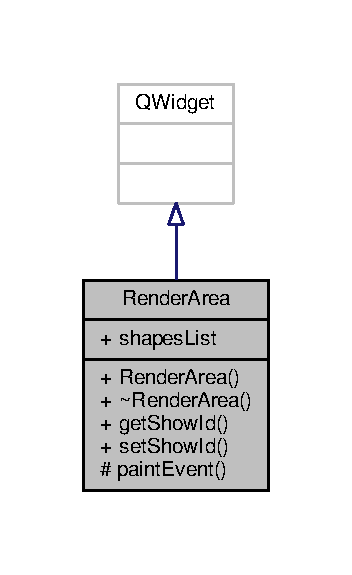
\includegraphics[width=169pt]{classRenderArea__inherit__graph}
\end{center}
\end{figure}


Collaboration diagram for Render\+Area\+:
\nopagebreak
\begin{figure}[H]
\begin{center}
\leavevmode
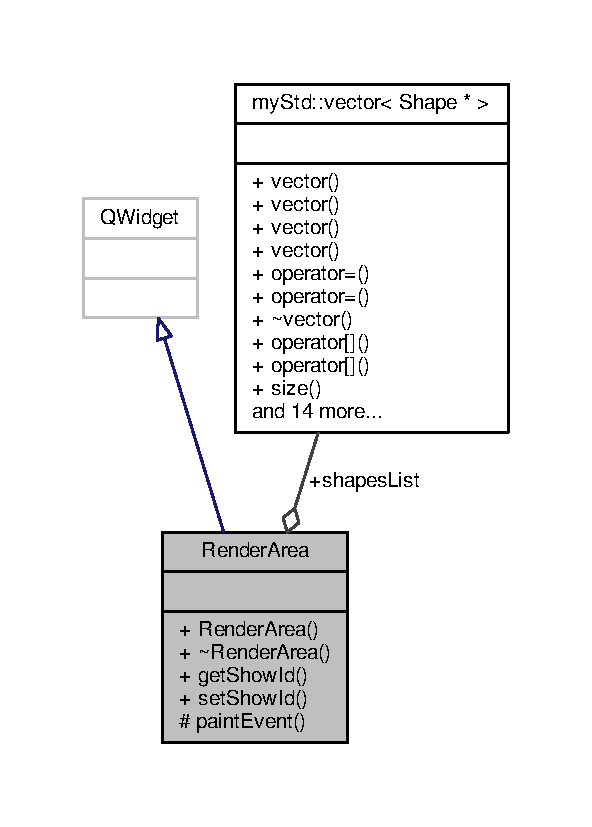
\includegraphics[width=284pt]{classRenderArea__coll__graph}
\end{center}
\end{figure}
\subsection*{Public Member Functions}
\begin{DoxyCompactItemize}
\item 
\hyperlink{classRenderArea_a71baad4c7f205d8f3c7fa2b1c7483448}{Render\+Area} (Q\+Widget $\ast$parent)
\begin{DoxyCompactList}\small\item\em \hyperlink{classRenderArea}{Render\+Area} constructor. \end{DoxyCompactList}\item 
virtual \hyperlink{classRenderArea_ade92334d3441242827d5a96fc9cd5f42}{$\sim$\+Render\+Area} ()
\item 
bool \hyperlink{classRenderArea_aff78d4f340f879fb5effa9830e4d77b9}{get\+Show\+Id} ()
\begin{DoxyCompactList}\small\item\em Gets a bool of whether to show the ids when rendering or not. \end{DoxyCompactList}\item 
const void \hyperlink{classRenderArea_a460a86b0f462ad0fd99ae30688754583}{set\+Show\+Id} (bool t)
\begin{DoxyCompactList}\small\item\em Sets the bool to signify if the shapes should be rendered with an id or not. \end{DoxyCompactList}\end{DoxyCompactItemize}
\subsection*{Public Attributes}
\begin{DoxyCompactItemize}
\item 
\hyperlink{classmyStd_1_1vector}{my\+Std\+::vector}$<$ \hyperlink{classShape}{Shape} $\ast$ $>$ \hyperlink{classRenderArea_a3502e321d5130cd9029c45c7238979e6}{shapes\+List}
\begin{DoxyCompactList}\small\item\em shapes\+List vector of Shape$\ast$ that \hyperlink{classRenderArea}{Render\+Area} draws \end{DoxyCompactList}\end{DoxyCompactItemize}
\subsection*{Protected Member Functions}
\begin{DoxyCompactItemize}
\item 
void \hyperlink{classRenderArea_ae9b5a1573f3b06590c717c7598ffaae4}{paint\+Event} (Q\+Paint\+Event $\ast$event) override
\begin{DoxyCompactList}\small\item\em paint\+Event calls draw on all of the shapes and draws them inside the \hyperlink{classRenderArea}{Render\+Area} \end{DoxyCompactList}\end{DoxyCompactItemize}


\subsection{Detailed Description}
The \hyperlink{classRenderArea}{Render\+Area} class provides the environment for drawing shapes. 

\subsection{Constructor \& Destructor Documentation}
\index{Render\+Area@{Render\+Area}!Render\+Area@{Render\+Area}}
\index{Render\+Area@{Render\+Area}!Render\+Area@{Render\+Area}}
\subsubsection[{\texorpdfstring{Render\+Area(\+Q\+Widget $\ast$parent)}{RenderArea(QWidget *parent)}}]{\setlength{\rightskip}{0pt plus 5cm}Render\+Area\+::\+Render\+Area (
\begin{DoxyParamCaption}
\item[{Q\+Widget $\ast$}]{parent}
\end{DoxyParamCaption}
)\hspace{0.3cm}{\ttfamily [inline]}}\hypertarget{classRenderArea_a71baad4c7f205d8f3c7fa2b1c7483448}{}\label{classRenderArea_a71baad4c7f205d8f3c7fa2b1c7483448}


\hyperlink{classRenderArea}{Render\+Area} constructor. 


\begin{DoxyParams}{Parameters}
{\em parent} & widget \\
\hline
\end{DoxyParams}
\index{Render\+Area@{Render\+Area}!````~Render\+Area@{$\sim$\+Render\+Area}}
\index{````~Render\+Area@{$\sim$\+Render\+Area}!Render\+Area@{Render\+Area}}
\subsubsection[{\texorpdfstring{$\sim$\+Render\+Area()}{~RenderArea()}}]{\setlength{\rightskip}{0pt plus 5cm}virtual Render\+Area\+::$\sim$\+Render\+Area (
\begin{DoxyParamCaption}
{}
\end{DoxyParamCaption}
)\hspace{0.3cm}{\ttfamily [inline]}, {\ttfamily [virtual]}}\hypertarget{classRenderArea_ade92334d3441242827d5a96fc9cd5f42}{}\label{classRenderArea_ade92334d3441242827d5a96fc9cd5f42}


\subsection{Member Function Documentation}
\index{Render\+Area@{Render\+Area}!get\+Show\+Id@{get\+Show\+Id}}
\index{get\+Show\+Id@{get\+Show\+Id}!Render\+Area@{Render\+Area}}
\subsubsection[{\texorpdfstring{get\+Show\+Id()}{getShowId()}}]{\setlength{\rightskip}{0pt plus 5cm}bool Render\+Area\+::get\+Show\+Id (
\begin{DoxyParamCaption}
{}
\end{DoxyParamCaption}
)\hspace{0.3cm}{\ttfamily [inline]}}\hypertarget{classRenderArea_aff78d4f340f879fb5effa9830e4d77b9}{}\label{classRenderArea_aff78d4f340f879fb5effa9830e4d77b9}


Gets a bool of whether to show the ids when rendering or not. 

\begin{DoxyReturn}{Returns}

\end{DoxyReturn}
\index{Render\+Area@{Render\+Area}!paint\+Event@{paint\+Event}}
\index{paint\+Event@{paint\+Event}!Render\+Area@{Render\+Area}}
\subsubsection[{\texorpdfstring{paint\+Event(\+Q\+Paint\+Event $\ast$event) override}{paintEvent(QPaintEvent *event) override}}]{\setlength{\rightskip}{0pt plus 5cm}void Render\+Area\+::paint\+Event (
\begin{DoxyParamCaption}
\item[{Q\+Paint\+Event $\ast$}]{event}
\end{DoxyParamCaption}
)\hspace{0.3cm}{\ttfamily [inline]}, {\ttfamily [override]}, {\ttfamily [protected]}}\hypertarget{classRenderArea_ae9b5a1573f3b06590c717c7598ffaae4}{}\label{classRenderArea_ae9b5a1573f3b06590c717c7598ffaae4}


paint\+Event calls draw on all of the shapes and draws them inside the \hyperlink{classRenderArea}{Render\+Area} 


\begin{DoxyParams}{Parameters}
{\em event} & Q\+Paint\+Event used to signify that it is a paint event \\
\hline
\end{DoxyParams}
\index{Render\+Area@{Render\+Area}!set\+Show\+Id@{set\+Show\+Id}}
\index{set\+Show\+Id@{set\+Show\+Id}!Render\+Area@{Render\+Area}}
\subsubsection[{\texorpdfstring{set\+Show\+Id(bool t)}{setShowId(bool t)}}]{\setlength{\rightskip}{0pt plus 5cm}const void Render\+Area\+::set\+Show\+Id (
\begin{DoxyParamCaption}
\item[{bool}]{t}
\end{DoxyParamCaption}
)\hspace{0.3cm}{\ttfamily [inline]}}\hypertarget{classRenderArea_a460a86b0f462ad0fd99ae30688754583}{}\label{classRenderArea_a460a86b0f462ad0fd99ae30688754583}


Sets the bool to signify if the shapes should be rendered with an id or not. 


\begin{DoxyParams}{Parameters}
{\em t} & bool of show\+Id condition \\
\hline
\end{DoxyParams}


\subsection{Member Data Documentation}
\index{Render\+Area@{Render\+Area}!shapes\+List@{shapes\+List}}
\index{shapes\+List@{shapes\+List}!Render\+Area@{Render\+Area}}
\subsubsection[{\texorpdfstring{shapes\+List}{shapesList}}]{\setlength{\rightskip}{0pt plus 5cm}{\bf my\+Std\+::vector}$<${\bf Shape}$\ast$$>$ Render\+Area\+::shapes\+List}\hypertarget{classRenderArea_a3502e321d5130cd9029c45c7238979e6}{}\label{classRenderArea_a3502e321d5130cd9029c45c7238979e6}


shapes\+List vector of Shape$\ast$ that \hyperlink{classRenderArea}{Render\+Area} draws 



The documentation for this class was generated from the following file\+:\begin{DoxyCompactItemize}
\item 
Group Project/\+Scrum\+Of\+The\+Earth/\hyperlink{renderarea_8h}{renderarea.\+h}\end{DoxyCompactItemize}

\hypertarget{classShape}{}\section{Shape Class Reference}
\label{classShape}\index{Shape@{Shape}}


Abstract Base Class for shapes that get rendered by the Q\+Painter.  




{\ttfamily \#include $<$shape.\+h$>$}



Inheritance diagram for Shape\+:\nopagebreak
\begin{figure}[H]
\begin{center}
\leavevmode
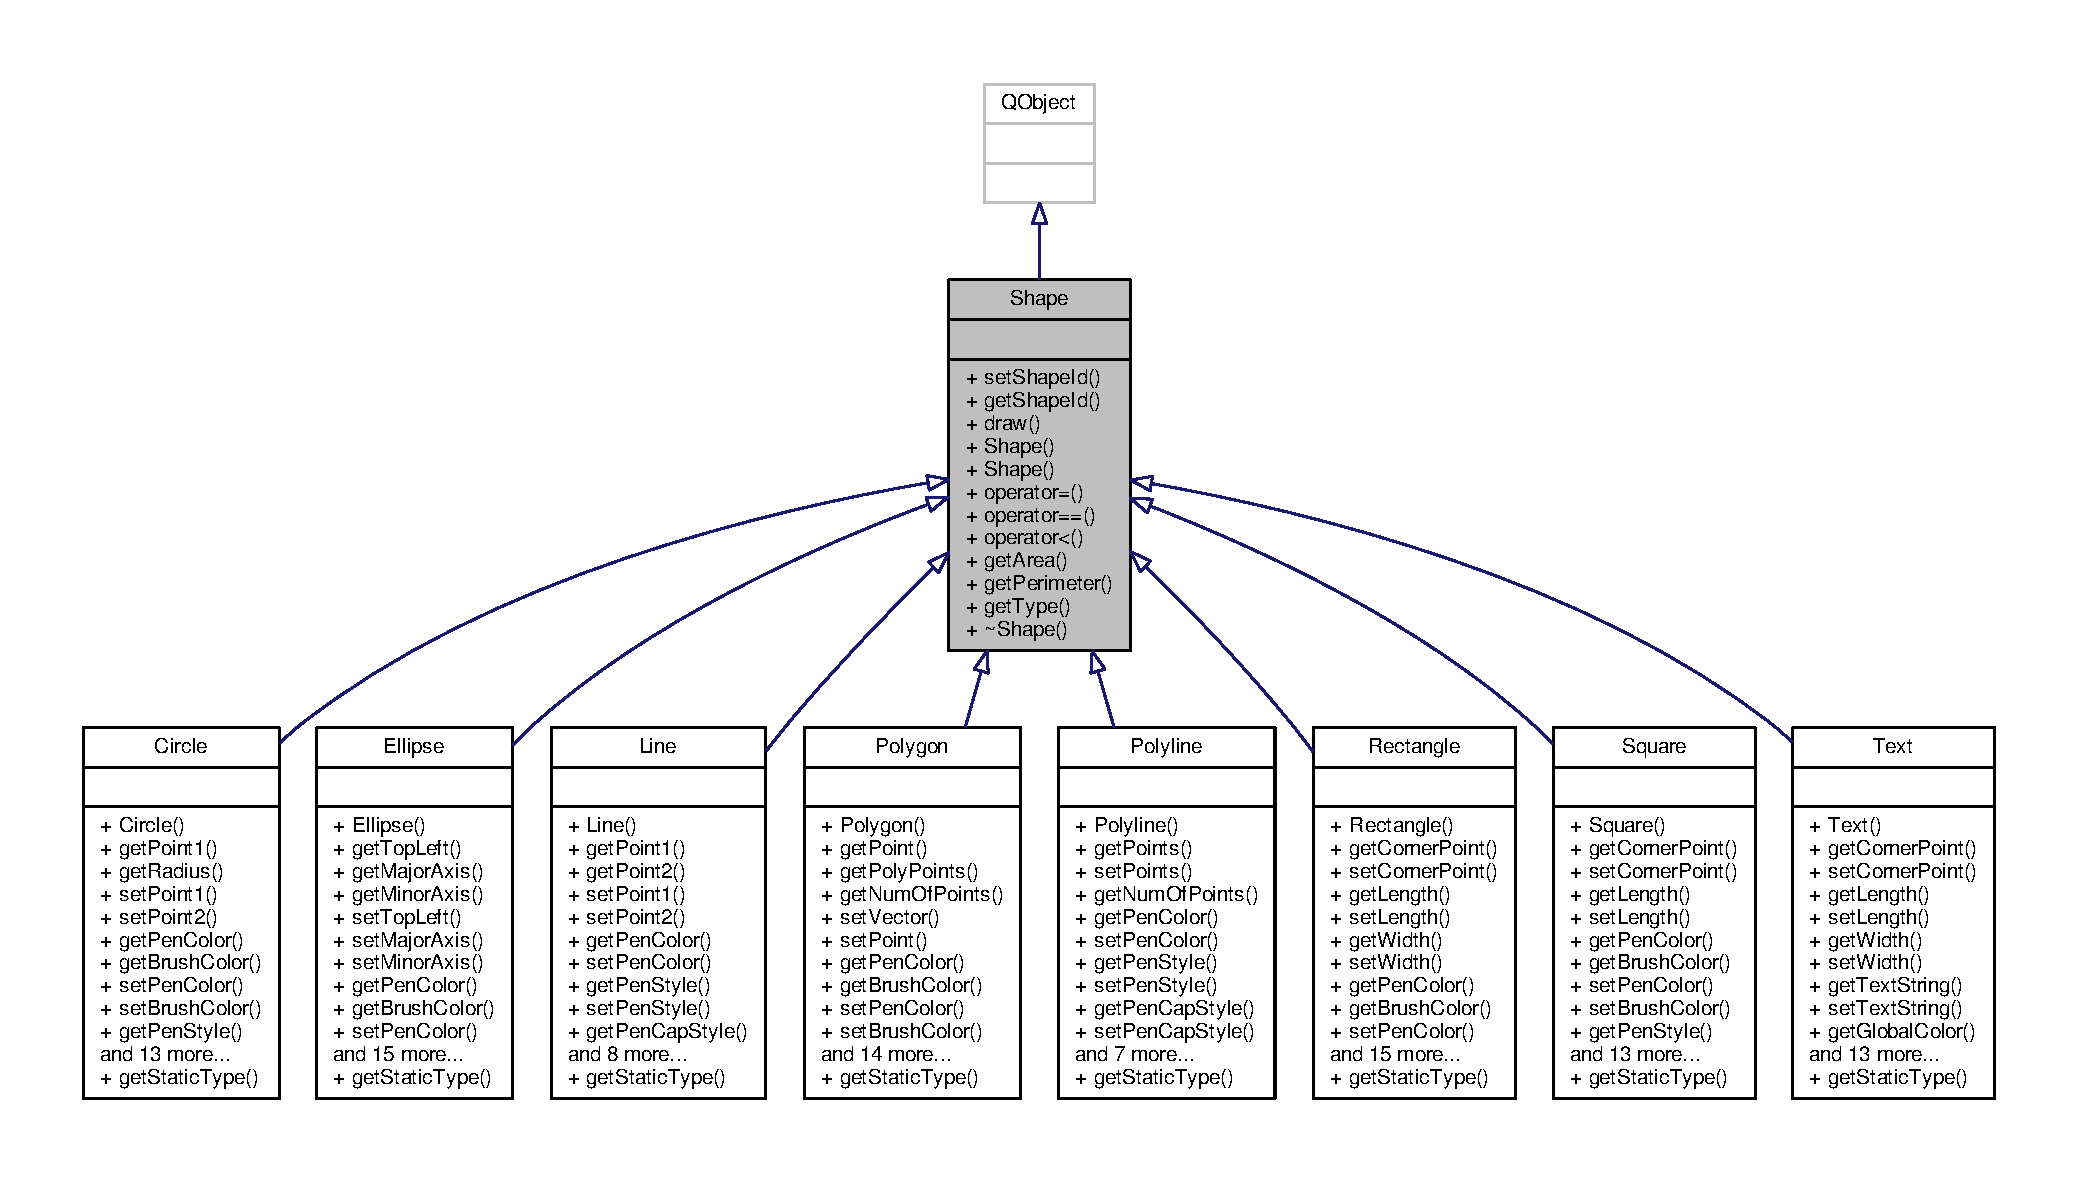
\includegraphics[width=350pt]{classShape__inherit__graph}
\end{center}
\end{figure}


Collaboration diagram for Shape\+:\nopagebreak
\begin{figure}[H]
\begin{center}
\leavevmode
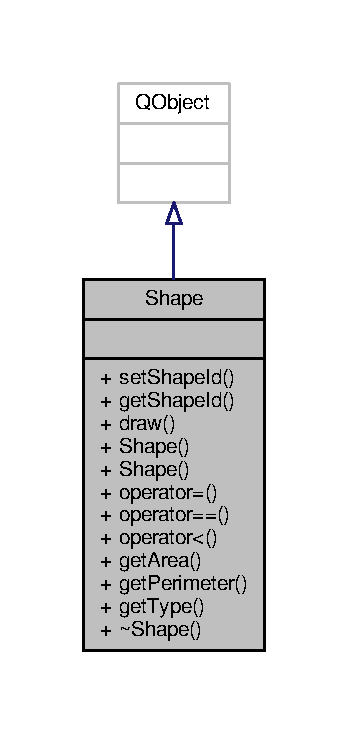
\includegraphics[width=167pt]{classShape__coll__graph}
\end{center}
\end{figure}
\subsection*{Public Member Functions}
\begin{DoxyCompactItemize}
\item 
void \hyperlink{classShape_a95f42a7833e43572d684455c2ee232ec}{set\+Shape\+Id} (unsigned int i)
\begin{DoxyCompactList}\small\item\em Sets the shape id to the given id. \end{DoxyCompactList}\item 
unsigned int \hyperlink{classShape_a3ac221427e91b0acc53a2f3764a8f01b}{get\+Shape\+Id} ()
\begin{DoxyCompactList}\small\item\em Gets the shape id of the \hyperlink{classShape}{Shape}. \end{DoxyCompactList}\item 
virtual void \hyperlink{classShape_a47dae32819e64fb32f3357f31978293f}{draw} (Q\+Painter \&, bool)=0
\begin{DoxyCompactList}\small\item\em Virtual function to draw shapes. \end{DoxyCompactList}\item 
\hyperlink{classShape_a3bb93456832521010106172a095e22ca}{Shape} (unsigned int id)
\begin{DoxyCompactList}\small\item\em \hyperlink{classShape}{Shape} constructor with id. \end{DoxyCompactList}\item 
\hyperlink{classShape_a44d91c7621d4d7af60fe3320a2e07279}{Shape} (const \hyperlink{classShape}{Shape} \&)=delete
\begin{DoxyCompactList}\small\item\em \hyperlink{classShape}{Shape} copy constructor (Disabled) \end{DoxyCompactList}\item 
\hyperlink{classShape}{Shape} \& \hyperlink{classShape_a9b9942917d6e6c359a8751156ed52423}{operator=} (const \hyperlink{classShape}{Shape} \&)=delete
\begin{DoxyCompactList}\small\item\em operator = copy assignment (disabled) \end{DoxyCompactList}\item 
bool \hyperlink{classShape_a1e81a927f61ea4d12daafc1d9295e00a}{operator==} (const \hyperlink{classShape}{Shape} \&s2)
\begin{DoxyCompactList}\small\item\em Checks to see if two \hyperlink{classShape}{Shape} ids are equal. \end{DoxyCompactList}\item 
bool \hyperlink{classShape_a0d2732ef366fa236a534351f6a0d96e5}{operator$<$} (const \hyperlink{classShape}{Shape} \&s2)
\begin{DoxyCompactList}\small\item\em Checks to see if \hyperlink{classShape}{Shape} 1\textquotesingle{}s id is less than \hyperlink{classShape}{Shape} 2\textquotesingle{}s id. \end{DoxyCompactList}\item 
virtual double \hyperlink{classShape_ac29f8bce0d038c84470028c6819a79ab}{get\+Area} ()
\begin{DoxyCompactList}\small\item\em Gets the area of the given shape. \end{DoxyCompactList}\item 
virtual double \hyperlink{classShape_a391744b6bce96df044139dcbd1ae0aa8}{get\+Perimeter} ()
\begin{DoxyCompactList}\small\item\em Gets the perimeter of the given shape. \end{DoxyCompactList}\item 
virtual int \hyperlink{classShape_a3d15adf2a1d746928f9be98105096eda}{get\+Type} ()=0
\begin{DoxyCompactList}\small\item\em Gets the type of the shape. \end{DoxyCompactList}\item 
virtual \hyperlink{classShape_ac3b9fc48965274893f25b18aa14ba665}{$\sim$\+Shape} ()
\begin{DoxyCompactList}\small\item\em $\sim$\+Shape \end{DoxyCompactList}\end{DoxyCompactItemize}


\subsection{Detailed Description}
Abstract Base Class for shapes that get rendered by the Q\+Painter. 

\subsection{Constructor \& Destructor Documentation}
\index{Shape@{Shape}!Shape@{Shape}}
\index{Shape@{Shape}!Shape@{Shape}}
\subsubsection[{\texorpdfstring{Shape(unsigned int id)}{Shape(unsigned int id)}}]{\setlength{\rightskip}{0pt plus 5cm}Shape\+::\+Shape (
\begin{DoxyParamCaption}
\item[{unsigned int}]{id}
\end{DoxyParamCaption}
)\hspace{0.3cm}{\ttfamily [inline]}}\hypertarget{classShape_a3bb93456832521010106172a095e22ca}{}\label{classShape_a3bb93456832521010106172a095e22ca}


\hyperlink{classShape}{Shape} constructor with id. 


\begin{DoxyParams}{Parameters}
{\em id} & \\
\hline
\end{DoxyParams}
\index{Shape@{Shape}!Shape@{Shape}}
\index{Shape@{Shape}!Shape@{Shape}}
\subsubsection[{\texorpdfstring{Shape(const Shape \&)=delete}{Shape(const Shape &)=delete}}]{\setlength{\rightskip}{0pt plus 5cm}Shape\+::\+Shape (
\begin{DoxyParamCaption}
\item[{const {\bf Shape} \&}]{}
\end{DoxyParamCaption}
)\hspace{0.3cm}{\ttfamily [delete]}}\hypertarget{classShape_a44d91c7621d4d7af60fe3320a2e07279}{}\label{classShape_a44d91c7621d4d7af60fe3320a2e07279}


\hyperlink{classShape}{Shape} copy constructor (Disabled) 

\index{Shape@{Shape}!````~Shape@{$\sim$\+Shape}}
\index{````~Shape@{$\sim$\+Shape}!Shape@{Shape}}
\subsubsection[{\texorpdfstring{$\sim$\+Shape()}{~Shape()}}]{\setlength{\rightskip}{0pt plus 5cm}virtual Shape\+::$\sim$\+Shape (
\begin{DoxyParamCaption}
{}
\end{DoxyParamCaption}
)\hspace{0.3cm}{\ttfamily [inline]}, {\ttfamily [virtual]}}\hypertarget{classShape_ac3b9fc48965274893f25b18aa14ba665}{}\label{classShape_ac3b9fc48965274893f25b18aa14ba665}


$\sim$\+Shape 



\subsection{Member Function Documentation}
\index{Shape@{Shape}!draw@{draw}}
\index{draw@{draw}!Shape@{Shape}}
\subsubsection[{\texorpdfstring{draw(\+Q\+Painter \&, bool)=0}{draw(QPainter &, bool)=0}}]{\setlength{\rightskip}{0pt plus 5cm}virtual void Shape\+::draw (
\begin{DoxyParamCaption}
\item[{Q\+Painter \&}]{, }
\item[{bool}]{}
\end{DoxyParamCaption}
)\hspace{0.3cm}{\ttfamily [pure virtual]}}\hypertarget{classShape_a47dae32819e64fb32f3357f31978293f}{}\label{classShape_a47dae32819e64fb32f3357f31978293f}


Virtual function to draw shapes. 



Implemented in \hyperlink{classCircle_aebc2ff1cc810905bc557d54e76aef936}{Circle}, \hyperlink{classEllipse_a807da0badc3cc332ba408e6d94333a36}{Ellipse}, \hyperlink{classRectangle_a6734cad19e207a212dcb042e1006a7f1}{Rectangle}, \hyperlink{classPolygon_a324e212e7f096a104f84fb854be50215}{Polygon}, \hyperlink{classSquare_acea142797dc1540a4fea5d343b7f1e82}{Square}, \hyperlink{classText_a54e8085e0b04abba6b4a09232ff21449}{Text}, \hyperlink{classLine_a3bcbb11a1d79a7f9a60cc1aac3ab1bb5}{Line}, and \hyperlink{classPolyline_ac5b5a4ac26b140a7dc30cc293638e3ee}{Polyline}.

\index{Shape@{Shape}!get\+Area@{get\+Area}}
\index{get\+Area@{get\+Area}!Shape@{Shape}}
\subsubsection[{\texorpdfstring{get\+Area()}{getArea()}}]{\setlength{\rightskip}{0pt plus 5cm}virtual double Shape\+::get\+Area (
\begin{DoxyParamCaption}
{}
\end{DoxyParamCaption}
)\hspace{0.3cm}{\ttfamily [inline]}, {\ttfamily [virtual]}}\hypertarget{classShape_ac29f8bce0d038c84470028c6819a79ab}{}\label{classShape_ac29f8bce0d038c84470028c6819a79ab}


Gets the area of the given shape. 

\begin{DoxyReturn}{Returns}
Area as a double 
\end{DoxyReturn}


Reimplemented in \hyperlink{classCircle_ae770cbdb3a0148a9db411fb3b0f87b9a}{Circle}, \hyperlink{classEllipse_aa9aff42aee3c6188e017dfa9d6a0590a}{Ellipse}, \hyperlink{classRectangle_a5405044e619a5ba1a52c0b9607c9f166}{Rectangle}, \hyperlink{classPolygon_a31c8c5320acfb934bce0441efb0fe837}{Polygon}, and \hyperlink{classSquare_a9a97feb159f85721b661b10ace6a8b3b}{Square}.

\index{Shape@{Shape}!get\+Perimeter@{get\+Perimeter}}
\index{get\+Perimeter@{get\+Perimeter}!Shape@{Shape}}
\subsubsection[{\texorpdfstring{get\+Perimeter()}{getPerimeter()}}]{\setlength{\rightskip}{0pt plus 5cm}virtual double Shape\+::get\+Perimeter (
\begin{DoxyParamCaption}
{}
\end{DoxyParamCaption}
)\hspace{0.3cm}{\ttfamily [inline]}, {\ttfamily [virtual]}}\hypertarget{classShape_a391744b6bce96df044139dcbd1ae0aa8}{}\label{classShape_a391744b6bce96df044139dcbd1ae0aa8}


Gets the perimeter of the given shape. 

\begin{DoxyReturn}{Returns}
Perimeter as a double 
\end{DoxyReturn}


Reimplemented in \hyperlink{classPolygon_a295ef7fe3b5ed921ae15a757680b159a}{Polygon}, \hyperlink{classCircle_af9a14f66b467788f8395ea587357a93f}{Circle}, \hyperlink{classEllipse_afc43182b486fb25e7ba9fd344cfee5d4}{Ellipse}, \hyperlink{classRectangle_aba6936b3c376465edff938cd4affc914}{Rectangle}, \hyperlink{classSquare_ae1d360c45a7970da83c3ad2acbf81dc2}{Square}, \hyperlink{classLine_ad63a55614d118000935e585f3551f630}{Line}, and \hyperlink{classPolyline_ad5425297b32d53a0f74eda253d4540f7}{Polyline}.

\index{Shape@{Shape}!get\+Shape\+Id@{get\+Shape\+Id}}
\index{get\+Shape\+Id@{get\+Shape\+Id}!Shape@{Shape}}
\subsubsection[{\texorpdfstring{get\+Shape\+Id()}{getShapeId()}}]{\setlength{\rightskip}{0pt plus 5cm}unsigned int Shape\+::get\+Shape\+Id (
\begin{DoxyParamCaption}
{}
\end{DoxyParamCaption}
)\hspace{0.3cm}{\ttfamily [inline]}}\hypertarget{classShape_a3ac221427e91b0acc53a2f3764a8f01b}{}\label{classShape_a3ac221427e91b0acc53a2f3764a8f01b}


Gets the shape id of the \hyperlink{classShape}{Shape}. 

\begin{DoxyReturn}{Returns}
id 
\end{DoxyReturn}
\index{Shape@{Shape}!get\+Type@{get\+Type}}
\index{get\+Type@{get\+Type}!Shape@{Shape}}
\subsubsection[{\texorpdfstring{get\+Type()=0}{getType()=0}}]{\setlength{\rightskip}{0pt plus 5cm}virtual int Shape\+::get\+Type (
\begin{DoxyParamCaption}
{}
\end{DoxyParamCaption}
)\hspace{0.3cm}{\ttfamily [pure virtual]}}\hypertarget{classShape_a3d15adf2a1d746928f9be98105096eda}{}\label{classShape_a3d15adf2a1d746928f9be98105096eda}


Gets the type of the shape. 

\begin{DoxyReturn}{Returns}
type as an int 
\end{DoxyReturn}


Implemented in \hyperlink{classCircle_ac13b29eb5095b4fd8e6c25ba50dd9131}{Circle}, \hyperlink{classEllipse_af8a6e2834d811a632d323cc3d9cb5b31}{Ellipse}, \hyperlink{classRectangle_a0098e1642c4ff1180c1243b802caca5a}{Rectangle}, \hyperlink{classPolygon_aa17e86eda9587c95a0e498e60033dfa3}{Polygon}, \hyperlink{classSquare_a1d225d79fc799bc98f9ad4d23e33a7d2}{Square}, \hyperlink{classText_a701eda01498e972823f4c833ed0e8811}{Text}, \hyperlink{classLine_a249b46f2c7dab063ac4754dbae444468}{Line}, and \hyperlink{classPolyline_a6138f6313141e81d989622806476c3d2}{Polyline}.

\index{Shape@{Shape}!operator$<$@{operator$<$}}
\index{operator$<$@{operator$<$}!Shape@{Shape}}
\subsubsection[{\texorpdfstring{operator$<$(const Shape \&s2)}{operator<(const Shape &s2)}}]{\setlength{\rightskip}{0pt plus 5cm}bool Shape\+::operator$<$ (
\begin{DoxyParamCaption}
\item[{const {\bf Shape} \&}]{s2}
\end{DoxyParamCaption}
)\hspace{0.3cm}{\ttfamily [inline]}}\hypertarget{classShape_a0d2732ef366fa236a534351f6a0d96e5}{}\label{classShape_a0d2732ef366fa236a534351f6a0d96e5}


Checks to see if \hyperlink{classShape}{Shape} 1\textquotesingle{}s id is less than \hyperlink{classShape}{Shape} 2\textquotesingle{}s id. 


\begin{DoxyParams}{Parameters}
{\em \hyperlink{classShape}{Shape}} & 2 \\
\hline
\end{DoxyParams}
\begin{DoxyReturn}{Returns}
result of comparison 
\end{DoxyReturn}
\index{Shape@{Shape}!operator=@{operator=}}
\index{operator=@{operator=}!Shape@{Shape}}
\subsubsection[{\texorpdfstring{operator=(const Shape \&)=delete}{operator=(const Shape &)=delete}}]{\setlength{\rightskip}{0pt plus 5cm}{\bf Shape}\& Shape\+::operator= (
\begin{DoxyParamCaption}
\item[{const {\bf Shape} \&}]{}
\end{DoxyParamCaption}
)\hspace{0.3cm}{\ttfamily [delete]}}\hypertarget{classShape_a9b9942917d6e6c359a8751156ed52423}{}\label{classShape_a9b9942917d6e6c359a8751156ed52423}


operator = copy assignment (disabled) 

\begin{DoxyReturn}{Returns}
This \hyperlink{classShape}{Shape} 
\end{DoxyReturn}
\index{Shape@{Shape}!operator==@{operator==}}
\index{operator==@{operator==}!Shape@{Shape}}
\subsubsection[{\texorpdfstring{operator==(const Shape \&s2)}{operator==(const Shape &s2)}}]{\setlength{\rightskip}{0pt plus 5cm}bool Shape\+::operator== (
\begin{DoxyParamCaption}
\item[{const {\bf Shape} \&}]{s2}
\end{DoxyParamCaption}
)\hspace{0.3cm}{\ttfamily [inline]}}\hypertarget{classShape_a1e81a927f61ea4d12daafc1d9295e00a}{}\label{classShape_a1e81a927f61ea4d12daafc1d9295e00a}


Checks to see if two \hyperlink{classShape}{Shape} ids are equal. 


\begin{DoxyParams}{Parameters}
{\em \hyperlink{classShape}{Shape}} & 2 \\
\hline
\end{DoxyParams}
\begin{DoxyReturn}{Returns}
result of comparison 
\end{DoxyReturn}
\index{Shape@{Shape}!set\+Shape\+Id@{set\+Shape\+Id}}
\index{set\+Shape\+Id@{set\+Shape\+Id}!Shape@{Shape}}
\subsubsection[{\texorpdfstring{set\+Shape\+Id(unsigned int i)}{setShapeId(unsigned int i)}}]{\setlength{\rightskip}{0pt plus 5cm}void Shape\+::set\+Shape\+Id (
\begin{DoxyParamCaption}
\item[{unsigned int}]{i}
\end{DoxyParamCaption}
)\hspace{0.3cm}{\ttfamily [inline]}}\hypertarget{classShape_a95f42a7833e43572d684455c2ee232ec}{}\label{classShape_a95f42a7833e43572d684455c2ee232ec}


Sets the shape id to the given id. 


\begin{DoxyParams}{Parameters}
{\em id} & \\
\hline
\end{DoxyParams}


The documentation for this class was generated from the following file\+:\begin{DoxyCompactItemize}
\item 
Group Project/\+Scrum\+Of\+The\+Earth/\hyperlink{shape_8h}{shape.\+h}\end{DoxyCompactItemize}

\hypertarget{classSquare}{}\section{Square Class Reference}
\label{classSquare}\index{Square@{Square}}


\hyperlink{classSquare}{Square} class that Q\+Painter can draw.  




{\ttfamily \#include $<$square.\+h$>$}



Inheritance diagram for Square\+:\nopagebreak
\begin{figure}[H]
\begin{center}
\leavevmode
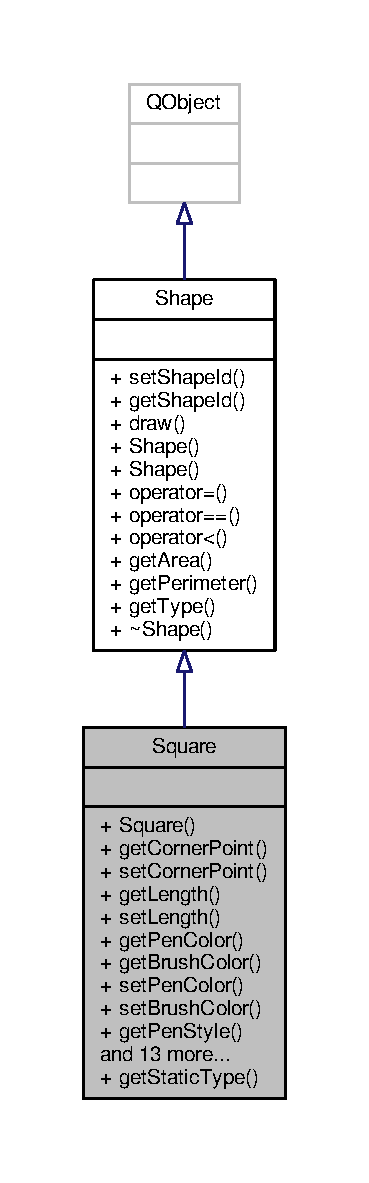
\includegraphics[height=550pt]{classSquare__inherit__graph}
\end{center}
\end{figure}


Collaboration diagram for Square\+:\nopagebreak
\begin{figure}[H]
\begin{center}
\leavevmode
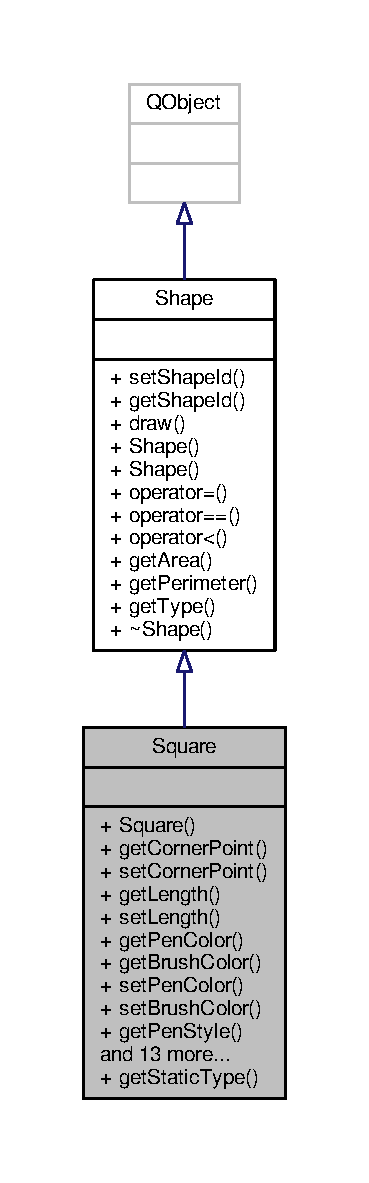
\includegraphics[height=550pt]{classSquare__coll__graph}
\end{center}
\end{figure}
\subsection*{Public Member Functions}
\begin{DoxyCompactItemize}
\item 
\hyperlink{classSquare_a2a877745d97b47cef1bb9473b183b074}{Square} (unsigned int, int, int, int, Qt\+::\+Global\+Color, Qt\+::\+Global\+Color, Qt\+::\+Pen\+Style, \hyperlink{shape__input__file__specs_8txt_a622efdcfef6789d4367974d2fe79019e}{Qt\+::\+Pen\+Cap\+Style}, \hyperlink{shape__input__file__specs_8txt_a007db2043c6063881de2043c05c9c4a9}{Qt\+::\+Pen\+Join\+Style}, \hyperlink{shape__input__file__specs_8txt_ad07f6fe6c28dcb0b3bdc324a72d0051f}{Qt\+::\+Brush\+Style}, int)
\begin{DoxyCompactList}\small\item\em \hyperlink{classSquare}{Square} all parameter constructor. \end{DoxyCompactList}\item 
Q\+Point \hyperlink{classSquare_a2fdd4544900c08c881c4bf4effe0b974}{get\+Corner\+Point} ()
\begin{DoxyCompactList}\small\item\em Gets the corner point of the square. \end{DoxyCompactList}\item 
void \hyperlink{classSquare_acfd205cb2fe02845e3ece8c9a1244943}{set\+Corner\+Point} (Q\+Point p1)
\begin{DoxyCompactList}\small\item\em Sets the corner point of the square to the given point. \end{DoxyCompactList}\item 
int \hyperlink{classSquare_a6d8a8d8ec4383ebefe4c274f189c6a79}{get\+Length} ()
\begin{DoxyCompactList}\small\item\em Gets the length of the square. \end{DoxyCompactList}\item 
void \hyperlink{classSquare_a6a04c5639dc3cd6501a1d80ad54f4171}{set\+Length} (int \hyperlink{shape__input__file__specs_8txt_a2e02238fe11bc76d2a69c565c7391545}{l})
\begin{DoxyCompactList}\small\item\em Sets the length of the square. \end{DoxyCompactList}\item 
Qt\+::\+Global\+Color \hyperlink{classSquare_a8e9f690383213cb901883ba0fd008818}{get\+Pen\+Color} ()
\begin{DoxyCompactList}\small\item\em Gets the pen color stored in this shape. \end{DoxyCompactList}\item 
Qt\+::\+Global\+Color \hyperlink{classSquare_a8f504b5de9fc6cbc7aedc90c6559cb58}{get\+Brush\+Color} ()
\begin{DoxyCompactList}\small\item\em Gets the Brush color stored in the \hyperlink{classShape}{Shape}. \end{DoxyCompactList}\item 
void \hyperlink{classSquare_aea0a3ccc55caacf339d9270d102b75c8}{set\+Pen\+Color} (Qt\+::\+Global\+Color pc)
\begin{DoxyCompactList}\small\item\em Sets the color of the pen to the given color. \end{DoxyCompactList}\item 
void \hyperlink{classSquare_ad649b56a35dba222144299a0a4e90483}{set\+Brush\+Color} (Qt\+::\+Global\+Color bc)
\begin{DoxyCompactList}\small\item\em Sets the color of the Brush to the given color. \end{DoxyCompactList}\item 
Qt\+::\+Pen\+Style \hyperlink{classSquare_a8acc57d1601adeb0800648799fc8beae}{get\+Pen\+Style} ()
\begin{DoxyCompactList}\small\item\em Gets the style of the pen stored in the shape. \end{DoxyCompactList}\item 
void \hyperlink{classSquare_a912efb5a33db0a697a275fccedf69523}{set\+Pen\+Style} (Qt\+::\+Pen\+Style ps)
\begin{DoxyCompactList}\small\item\em Sets the style of the pen to the given style. \end{DoxyCompactList}\item 
\hyperlink{shape__input__file__specs_8txt_a622efdcfef6789d4367974d2fe79019e}{Qt\+::\+Pen\+Cap\+Style} \hyperlink{classSquare_a3b91e8b3b03d2a6125836a5477cfc9be}{get\+Pen\+Cap\+Style} ()
\begin{DoxyCompactList}\small\item\em Gets the pen cap style that is stored in this \hyperlink{classShape}{Shape}. \end{DoxyCompactList}\item 
void \hyperlink{classSquare_a5b9e32153640bdb937b1140f1c45083e}{set\+Pen\+Cap\+Style} (\hyperlink{shape__input__file__specs_8txt_a622efdcfef6789d4367974d2fe79019e}{Qt\+::\+Pen\+Cap\+Style} pcs)
\begin{DoxyCompactList}\small\item\em Sets the Pen Cap Style to the given Pen Cap Style. \end{DoxyCompactList}\item 
\hyperlink{shape__input__file__specs_8txt_a007db2043c6063881de2043c05c9c4a9}{Qt\+::\+Pen\+Join\+Style} \hyperlink{classSquare_a6fd69d97012e009ffea95e457f3a845e}{get\+Pen\+Join\+Style} ()
\begin{DoxyCompactList}\small\item\em Gets the Pen Join Style. \end{DoxyCompactList}\item 
void \hyperlink{classSquare_a51ebefc5fc56435612188060b6088bd7}{set\+Pen\+Join\+Style} (\hyperlink{shape__input__file__specs_8txt_a007db2043c6063881de2043c05c9c4a9}{Qt\+::\+Pen\+Join\+Style} pjs)
\begin{DoxyCompactList}\small\item\em Sets the pen join style to the given style. \end{DoxyCompactList}\item 
\hyperlink{shape__input__file__specs_8txt_ad07f6fe6c28dcb0b3bdc324a72d0051f}{Qt\+::\+Brush\+Style} \hyperlink{classSquare_a63e121e72afaba2766f24a0d8816974f}{get\+Brush\+Style} ()
\begin{DoxyCompactList}\small\item\em Gets the Brush Style. \end{DoxyCompactList}\item 
void \hyperlink{classSquare_aec04ffe7d0b567be4a7221013add1d6d}{set\+Brush\+Style} (\hyperlink{shape__input__file__specs_8txt_ad07f6fe6c28dcb0b3bdc324a72d0051f}{Qt\+::\+Brush\+Style} bs)
\begin{DoxyCompactList}\small\item\em Sets the Brush Style to the given Brush Style. \end{DoxyCompactList}\item 
int \hyperlink{classSquare_ac6b3bedb6d43e5059840221331d802fd}{get\+Pen\+Width} ()
\begin{DoxyCompactList}\small\item\em Gets the width of the pen. \end{DoxyCompactList}\item 
void \hyperlink{classSquare_a26697e2c607e6cbda21a63e0f292e5e6}{set\+Pen\+Width} (int pw)
\begin{DoxyCompactList}\small\item\em Sets the width of the pen to the given width. \end{DoxyCompactList}\item 
virtual void \hyperlink{classSquare_acea142797dc1540a4fea5d343b7f1e82}{draw} (Q\+Painter \&, bool)
\begin{DoxyCompactList}\small\item\em Virtual function to draw shapes. \end{DoxyCompactList}\item 
virtual int \hyperlink{classSquare_a1d225d79fc799bc98f9ad4d23e33a7d2}{get\+Type} ()
\begin{DoxyCompactList}\small\item\em Gets the type of the shape. \end{DoxyCompactList}\item 
virtual double \hyperlink{classSquare_a9a97feb159f85721b661b10ace6a8b3b}{get\+Area} ()
\begin{DoxyCompactList}\small\item\em Gets the area of the given shape. \end{DoxyCompactList}\item 
virtual double \hyperlink{classSquare_ae1d360c45a7970da83c3ad2acbf81dc2}{get\+Perimeter} ()
\begin{DoxyCompactList}\small\item\em Gets the perimeter of the given shape. \end{DoxyCompactList}\end{DoxyCompactItemize}
\subsection*{Static Public Member Functions}
\begin{DoxyCompactItemize}
\item 
static int \hyperlink{classSquare_a5d6e510d07f465fefdd1cdbbd041db2f}{get\+Static\+Type} ()
\begin{DoxyCompactList}\small\item\em gets the Type of object \end{DoxyCompactList}\end{DoxyCompactItemize}


\subsection{Detailed Description}
\hyperlink{classSquare}{Square} class that Q\+Painter can draw. 

\subsection{Constructor \& Destructor Documentation}
\index{Square@{Square}!Square@{Square}}
\index{Square@{Square}!Square@{Square}}
\subsubsection[{\texorpdfstring{Square(unsigned int, int, int, int, Qt\+::\+Global\+Color, Qt\+::\+Global\+Color, Qt\+::\+Pen\+Style, Qt\+::\+Pen\+Cap\+Style, Qt\+::\+Pen\+Join\+Style, Qt\+::\+Brush\+Style, int)}{Square(unsigned int, int, int, int, Qt::GlobalColor, Qt::GlobalColor, Qt::PenStyle, Qt::PenCapStyle, Qt::PenJoinStyle, Qt::BrushStyle, int)}}]{\setlength{\rightskip}{0pt plus 5cm}Square\+::\+Square (
\begin{DoxyParamCaption}
\item[{unsigned int}]{i, }
\item[{int}]{x, }
\item[{int}]{y, }
\item[{int}]{l, }
\item[{Qt\+::\+Global\+Color}]{pc, }
\item[{Qt\+::\+Global\+Color}]{bc, }
\item[{Qt\+::\+Pen\+Style}]{ps, }
\item[{{\bf Qt\+::\+Pen\+Cap\+Style}}]{pcs, }
\item[{{\bf Qt\+::\+Pen\+Join\+Style}}]{pjs, }
\item[{{\bf Qt\+::\+Brush\+Style}}]{bs, }
\item[{int}]{pw}
\end{DoxyParamCaption}
)}\hypertarget{classSquare_a2a877745d97b47cef1bb9473b183b074}{}\label{classSquare_a2a877745d97b47cef1bb9473b183b074}


\hyperlink{classSquare}{Square} all parameter constructor. 



\subsection{Member Function Documentation}
\index{Square@{Square}!draw@{draw}}
\index{draw@{draw}!Square@{Square}}
\subsubsection[{\texorpdfstring{draw(\+Q\+Painter \&, bool)}{draw(QPainter &, bool)}}]{\setlength{\rightskip}{0pt plus 5cm}void Square\+::draw (
\begin{DoxyParamCaption}
\item[{Q\+Painter \&}]{, }
\item[{bool}]{}
\end{DoxyParamCaption}
)\hspace{0.3cm}{\ttfamily [virtual]}}\hypertarget{classSquare_acea142797dc1540a4fea5d343b7f1e82}{}\label{classSquare_acea142797dc1540a4fea5d343b7f1e82}


Virtual function to draw shapes. 



Implements \hyperlink{classShape_a47dae32819e64fb32f3357f31978293f}{Shape}.

\index{Square@{Square}!get\+Area@{get\+Area}}
\index{get\+Area@{get\+Area}!Square@{Square}}
\subsubsection[{\texorpdfstring{get\+Area()}{getArea()}}]{\setlength{\rightskip}{0pt plus 5cm}virtual double Square\+::get\+Area (
\begin{DoxyParamCaption}
{}
\end{DoxyParamCaption}
)\hspace{0.3cm}{\ttfamily [inline]}, {\ttfamily [virtual]}}\hypertarget{classSquare_a9a97feb159f85721b661b10ace6a8b3b}{}\label{classSquare_a9a97feb159f85721b661b10ace6a8b3b}


Gets the area of the given shape. 

\begin{DoxyReturn}{Returns}
Area as a double 
\end{DoxyReturn}


Reimplemented from \hyperlink{classShape_ac29f8bce0d038c84470028c6819a79ab}{Shape}.

\index{Square@{Square}!get\+Brush\+Color@{get\+Brush\+Color}}
\index{get\+Brush\+Color@{get\+Brush\+Color}!Square@{Square}}
\subsubsection[{\texorpdfstring{get\+Brush\+Color()}{getBrushColor()}}]{\setlength{\rightskip}{0pt plus 5cm}Qt\+::\+Global\+Color Square\+::get\+Brush\+Color (
\begin{DoxyParamCaption}
{}
\end{DoxyParamCaption}
)\hspace{0.3cm}{\ttfamily [inline]}}\hypertarget{classSquare_a8f504b5de9fc6cbc7aedc90c6559cb58}{}\label{classSquare_a8f504b5de9fc6cbc7aedc90c6559cb58}


Gets the Brush color stored in the \hyperlink{classShape}{Shape}. 

\begin{DoxyReturn}{Returns}
Color of the Brush 
\end{DoxyReturn}
\index{Square@{Square}!get\+Brush\+Style@{get\+Brush\+Style}}
\index{get\+Brush\+Style@{get\+Brush\+Style}!Square@{Square}}
\subsubsection[{\texorpdfstring{get\+Brush\+Style()}{getBrushStyle()}}]{\setlength{\rightskip}{0pt plus 5cm}{\bf Qt\+::\+Brush\+Style} Square\+::get\+Brush\+Style (
\begin{DoxyParamCaption}
{}
\end{DoxyParamCaption}
)\hspace{0.3cm}{\ttfamily [inline]}}\hypertarget{classSquare_a63e121e72afaba2766f24a0d8816974f}{}\label{classSquare_a63e121e72afaba2766f24a0d8816974f}


Gets the Brush Style. 

\begin{DoxyReturn}{Returns}
Brush\+Style 
\end{DoxyReturn}
\index{Square@{Square}!get\+Corner\+Point@{get\+Corner\+Point}}
\index{get\+Corner\+Point@{get\+Corner\+Point}!Square@{Square}}
\subsubsection[{\texorpdfstring{get\+Corner\+Point()}{getCornerPoint()}}]{\setlength{\rightskip}{0pt plus 5cm}Q\+Point Square\+::get\+Corner\+Point (
\begin{DoxyParamCaption}
{}
\end{DoxyParamCaption}
)\hspace{0.3cm}{\ttfamily [inline]}}\hypertarget{classSquare_a2fdd4544900c08c881c4bf4effe0b974}{}\label{classSquare_a2fdd4544900c08c881c4bf4effe0b974}


Gets the corner point of the square. 

\begin{DoxyReturn}{Returns}
Q\+Point of the top left corner 
\end{DoxyReturn}
\index{Square@{Square}!get\+Length@{get\+Length}}
\index{get\+Length@{get\+Length}!Square@{Square}}
\subsubsection[{\texorpdfstring{get\+Length()}{getLength()}}]{\setlength{\rightskip}{0pt plus 5cm}int Square\+::get\+Length (
\begin{DoxyParamCaption}
{}
\end{DoxyParamCaption}
)\hspace{0.3cm}{\ttfamily [inline]}}\hypertarget{classSquare_a6d8a8d8ec4383ebefe4c274f189c6a79}{}\label{classSquare_a6d8a8d8ec4383ebefe4c274f189c6a79}


Gets the length of the square. 

\begin{DoxyReturn}{Returns}
int length of square 
\end{DoxyReturn}
\index{Square@{Square}!get\+Pen\+Cap\+Style@{get\+Pen\+Cap\+Style}}
\index{get\+Pen\+Cap\+Style@{get\+Pen\+Cap\+Style}!Square@{Square}}
\subsubsection[{\texorpdfstring{get\+Pen\+Cap\+Style()}{getPenCapStyle()}}]{\setlength{\rightskip}{0pt plus 5cm}{\bf Qt\+::\+Pen\+Cap\+Style} Square\+::get\+Pen\+Cap\+Style (
\begin{DoxyParamCaption}
{}
\end{DoxyParamCaption}
)\hspace{0.3cm}{\ttfamily [inline]}}\hypertarget{classSquare_a3b91e8b3b03d2a6125836a5477cfc9be}{}\label{classSquare_a3b91e8b3b03d2a6125836a5477cfc9be}


Gets the pen cap style that is stored in this \hyperlink{classShape}{Shape}. 

\begin{DoxyReturn}{Returns}
Pen\+Cap\+Style 
\end{DoxyReturn}
\index{Square@{Square}!get\+Pen\+Color@{get\+Pen\+Color}}
\index{get\+Pen\+Color@{get\+Pen\+Color}!Square@{Square}}
\subsubsection[{\texorpdfstring{get\+Pen\+Color()}{getPenColor()}}]{\setlength{\rightskip}{0pt plus 5cm}Qt\+::\+Global\+Color Square\+::get\+Pen\+Color (
\begin{DoxyParamCaption}
{}
\end{DoxyParamCaption}
)\hspace{0.3cm}{\ttfamily [inline]}}\hypertarget{classSquare_a8e9f690383213cb901883ba0fd008818}{}\label{classSquare_a8e9f690383213cb901883ba0fd008818}


Gets the pen color stored in this shape. 

\begin{DoxyReturn}{Returns}
Color of the pen 
\end{DoxyReturn}
\index{Square@{Square}!get\+Pen\+Join\+Style@{get\+Pen\+Join\+Style}}
\index{get\+Pen\+Join\+Style@{get\+Pen\+Join\+Style}!Square@{Square}}
\subsubsection[{\texorpdfstring{get\+Pen\+Join\+Style()}{getPenJoinStyle()}}]{\setlength{\rightskip}{0pt plus 5cm}{\bf Qt\+::\+Pen\+Join\+Style} Square\+::get\+Pen\+Join\+Style (
\begin{DoxyParamCaption}
{}
\end{DoxyParamCaption}
)\hspace{0.3cm}{\ttfamily [inline]}}\hypertarget{classSquare_a6fd69d97012e009ffea95e457f3a845e}{}\label{classSquare_a6fd69d97012e009ffea95e457f3a845e}


Gets the Pen Join Style. 

\begin{DoxyReturn}{Returns}
Pen\+Join\+Style 
\end{DoxyReturn}
\index{Square@{Square}!get\+Pen\+Style@{get\+Pen\+Style}}
\index{get\+Pen\+Style@{get\+Pen\+Style}!Square@{Square}}
\subsubsection[{\texorpdfstring{get\+Pen\+Style()}{getPenStyle()}}]{\setlength{\rightskip}{0pt plus 5cm}Qt\+::\+Pen\+Style Square\+::get\+Pen\+Style (
\begin{DoxyParamCaption}
{}
\end{DoxyParamCaption}
)\hspace{0.3cm}{\ttfamily [inline]}}\hypertarget{classSquare_a8acc57d1601adeb0800648799fc8beae}{}\label{classSquare_a8acc57d1601adeb0800648799fc8beae}


Gets the style of the pen stored in the shape. 

\begin{DoxyReturn}{Returns}
Style of the pen 
\end{DoxyReturn}
\index{Square@{Square}!get\+Pen\+Width@{get\+Pen\+Width}}
\index{get\+Pen\+Width@{get\+Pen\+Width}!Square@{Square}}
\subsubsection[{\texorpdfstring{get\+Pen\+Width()}{getPenWidth()}}]{\setlength{\rightskip}{0pt plus 5cm}int Square\+::get\+Pen\+Width (
\begin{DoxyParamCaption}
{}
\end{DoxyParamCaption}
)\hspace{0.3cm}{\ttfamily [inline]}}\hypertarget{classSquare_ac6b3bedb6d43e5059840221331d802fd}{}\label{classSquare_ac6b3bedb6d43e5059840221331d802fd}


Gets the width of the pen. 

\begin{DoxyReturn}{Returns}
pen\+Width 
\end{DoxyReturn}
\index{Square@{Square}!get\+Perimeter@{get\+Perimeter}}
\index{get\+Perimeter@{get\+Perimeter}!Square@{Square}}
\subsubsection[{\texorpdfstring{get\+Perimeter()}{getPerimeter()}}]{\setlength{\rightskip}{0pt plus 5cm}virtual double Square\+::get\+Perimeter (
\begin{DoxyParamCaption}
{}
\end{DoxyParamCaption}
)\hspace{0.3cm}{\ttfamily [inline]}, {\ttfamily [virtual]}}\hypertarget{classSquare_ae1d360c45a7970da83c3ad2acbf81dc2}{}\label{classSquare_ae1d360c45a7970da83c3ad2acbf81dc2}


Gets the perimeter of the given shape. 

\begin{DoxyReturn}{Returns}
Perimeter as a double 
\end{DoxyReturn}


Reimplemented from \hyperlink{classShape_a391744b6bce96df044139dcbd1ae0aa8}{Shape}.

\index{Square@{Square}!get\+Static\+Type@{get\+Static\+Type}}
\index{get\+Static\+Type@{get\+Static\+Type}!Square@{Square}}
\subsubsection[{\texorpdfstring{get\+Static\+Type()}{getStaticType()}}]{\setlength{\rightskip}{0pt plus 5cm}static int Square\+::get\+Static\+Type (
\begin{DoxyParamCaption}
{}
\end{DoxyParamCaption}
)\hspace{0.3cm}{\ttfamily [inline]}, {\ttfamily [static]}}\hypertarget{classSquare_a5d6e510d07f465fefdd1cdbbd041db2f}{}\label{classSquare_a5d6e510d07f465fefdd1cdbbd041db2f}


gets the Type of object 

\begin{DoxyReturn}{Returns}
Type as int 
\end{DoxyReturn}
\index{Square@{Square}!get\+Type@{get\+Type}}
\index{get\+Type@{get\+Type}!Square@{Square}}
\subsubsection[{\texorpdfstring{get\+Type()}{getType()}}]{\setlength{\rightskip}{0pt plus 5cm}virtual int Square\+::get\+Type (
\begin{DoxyParamCaption}
{}
\end{DoxyParamCaption}
)\hspace{0.3cm}{\ttfamily [inline]}, {\ttfamily [virtual]}}\hypertarget{classSquare_a1d225d79fc799bc98f9ad4d23e33a7d2}{}\label{classSquare_a1d225d79fc799bc98f9ad4d23e33a7d2}


Gets the type of the shape. 

\begin{DoxyReturn}{Returns}
type as an int 
\end{DoxyReturn}


Implements \hyperlink{classShape_a3d15adf2a1d746928f9be98105096eda}{Shape}.

\index{Square@{Square}!set\+Brush\+Color@{set\+Brush\+Color}}
\index{set\+Brush\+Color@{set\+Brush\+Color}!Square@{Square}}
\subsubsection[{\texorpdfstring{set\+Brush\+Color(\+Qt\+::\+Global\+Color bc)}{setBrushColor(Qt::GlobalColor bc)}}]{\setlength{\rightskip}{0pt plus 5cm}void Square\+::set\+Brush\+Color (
\begin{DoxyParamCaption}
\item[{Qt\+::\+Global\+Color}]{bc}
\end{DoxyParamCaption}
)\hspace{0.3cm}{\ttfamily [inline]}}\hypertarget{classSquare_ad649b56a35dba222144299a0a4e90483}{}\label{classSquare_ad649b56a35dba222144299a0a4e90483}


Sets the color of the Brush to the given color. 


\begin{DoxyParams}{Parameters}
{\em brush\+Color} & \\
\hline
\end{DoxyParams}
\index{Square@{Square}!set\+Brush\+Style@{set\+Brush\+Style}}
\index{set\+Brush\+Style@{set\+Brush\+Style}!Square@{Square}}
\subsubsection[{\texorpdfstring{set\+Brush\+Style(\+Qt\+::\+Brush\+Style bs)}{setBrushStyle(Qt::BrushStyle bs)}}]{\setlength{\rightskip}{0pt plus 5cm}void Square\+::set\+Brush\+Style (
\begin{DoxyParamCaption}
\item[{{\bf Qt\+::\+Brush\+Style}}]{bs}
\end{DoxyParamCaption}
)\hspace{0.3cm}{\ttfamily [inline]}}\hypertarget{classSquare_aec04ffe7d0b567be4a7221013add1d6d}{}\label{classSquare_aec04ffe7d0b567be4a7221013add1d6d}


Sets the Brush Style to the given Brush Style. 


\begin{DoxyParams}{Parameters}
{\em brush\+Style} & \\
\hline
\end{DoxyParams}
\index{Square@{Square}!set\+Corner\+Point@{set\+Corner\+Point}}
\index{set\+Corner\+Point@{set\+Corner\+Point}!Square@{Square}}
\subsubsection[{\texorpdfstring{set\+Corner\+Point(\+Q\+Point p1)}{setCornerPoint(QPoint p1)}}]{\setlength{\rightskip}{0pt plus 5cm}void Square\+::set\+Corner\+Point (
\begin{DoxyParamCaption}
\item[{Q\+Point}]{p1}
\end{DoxyParamCaption}
)\hspace{0.3cm}{\ttfamily [inline]}}\hypertarget{classSquare_acfd205cb2fe02845e3ece8c9a1244943}{}\label{classSquare_acfd205cb2fe02845e3ece8c9a1244943}


Sets the corner point of the square to the given point. 


\begin{DoxyParams}{Parameters}
{\em p1} & Q\+Point of top left corner \\
\hline
\end{DoxyParams}
\index{Square@{Square}!set\+Length@{set\+Length}}
\index{set\+Length@{set\+Length}!Square@{Square}}
\subsubsection[{\texorpdfstring{set\+Length(int l)}{setLength(int l)}}]{\setlength{\rightskip}{0pt plus 5cm}void Square\+::set\+Length (
\begin{DoxyParamCaption}
\item[{int}]{l}
\end{DoxyParamCaption}
)\hspace{0.3cm}{\ttfamily [inline]}}\hypertarget{classSquare_a6a04c5639dc3cd6501a1d80ad54f4171}{}\label{classSquare_a6a04c5639dc3cd6501a1d80ad54f4171}


Sets the length of the square. 


\begin{DoxyParams}{Parameters}
{\em l} & length of square \\
\hline
\end{DoxyParams}
\index{Square@{Square}!set\+Pen\+Cap\+Style@{set\+Pen\+Cap\+Style}}
\index{set\+Pen\+Cap\+Style@{set\+Pen\+Cap\+Style}!Square@{Square}}
\subsubsection[{\texorpdfstring{set\+Pen\+Cap\+Style(\+Qt\+::\+Pen\+Cap\+Style pcs)}{setPenCapStyle(Qt::PenCapStyle pcs)}}]{\setlength{\rightskip}{0pt plus 5cm}void Square\+::set\+Pen\+Cap\+Style (
\begin{DoxyParamCaption}
\item[{{\bf Qt\+::\+Pen\+Cap\+Style}}]{pcs}
\end{DoxyParamCaption}
)\hspace{0.3cm}{\ttfamily [inline]}}\hypertarget{classSquare_a5b9e32153640bdb937b1140f1c45083e}{}\label{classSquare_a5b9e32153640bdb937b1140f1c45083e}


Sets the Pen Cap Style to the given Pen Cap Style. 


\begin{DoxyParams}{Parameters}
{\em pen\+Cap\+Style} & \\
\hline
\end{DoxyParams}
\index{Square@{Square}!set\+Pen\+Color@{set\+Pen\+Color}}
\index{set\+Pen\+Color@{set\+Pen\+Color}!Square@{Square}}
\subsubsection[{\texorpdfstring{set\+Pen\+Color(\+Qt\+::\+Global\+Color pc)}{setPenColor(Qt::GlobalColor pc)}}]{\setlength{\rightskip}{0pt plus 5cm}void Square\+::set\+Pen\+Color (
\begin{DoxyParamCaption}
\item[{Qt\+::\+Global\+Color}]{pc}
\end{DoxyParamCaption}
)\hspace{0.3cm}{\ttfamily [inline]}}\hypertarget{classSquare_aea0a3ccc55caacf339d9270d102b75c8}{}\label{classSquare_aea0a3ccc55caacf339d9270d102b75c8}


Sets the color of the pen to the given color. 


\begin{DoxyParams}{Parameters}
{\em pen\+Color} & \\
\hline
\end{DoxyParams}
\index{Square@{Square}!set\+Pen\+Join\+Style@{set\+Pen\+Join\+Style}}
\index{set\+Pen\+Join\+Style@{set\+Pen\+Join\+Style}!Square@{Square}}
\subsubsection[{\texorpdfstring{set\+Pen\+Join\+Style(\+Qt\+::\+Pen\+Join\+Style pjs)}{setPenJoinStyle(Qt::PenJoinStyle pjs)}}]{\setlength{\rightskip}{0pt plus 5cm}void Square\+::set\+Pen\+Join\+Style (
\begin{DoxyParamCaption}
\item[{{\bf Qt\+::\+Pen\+Join\+Style}}]{pjs}
\end{DoxyParamCaption}
)\hspace{0.3cm}{\ttfamily [inline]}}\hypertarget{classSquare_a51ebefc5fc56435612188060b6088bd7}{}\label{classSquare_a51ebefc5fc56435612188060b6088bd7}


Sets the pen join style to the given style. 


\begin{DoxyParams}{Parameters}
{\em pen\+Join\+Style} & \\
\hline
\end{DoxyParams}
\index{Square@{Square}!set\+Pen\+Style@{set\+Pen\+Style}}
\index{set\+Pen\+Style@{set\+Pen\+Style}!Square@{Square}}
\subsubsection[{\texorpdfstring{set\+Pen\+Style(\+Qt\+::\+Pen\+Style ps)}{setPenStyle(Qt::PenStyle ps)}}]{\setlength{\rightskip}{0pt plus 5cm}void Square\+::set\+Pen\+Style (
\begin{DoxyParamCaption}
\item[{Qt\+::\+Pen\+Style}]{ps}
\end{DoxyParamCaption}
)\hspace{0.3cm}{\ttfamily [inline]}}\hypertarget{classSquare_a912efb5a33db0a697a275fccedf69523}{}\label{classSquare_a912efb5a33db0a697a275fccedf69523}


Sets the style of the pen to the given style. 


\begin{DoxyParams}{Parameters}
{\em pen\+Style} & \\
\hline
\end{DoxyParams}
\index{Square@{Square}!set\+Pen\+Width@{set\+Pen\+Width}}
\index{set\+Pen\+Width@{set\+Pen\+Width}!Square@{Square}}
\subsubsection[{\texorpdfstring{set\+Pen\+Width(int pw)}{setPenWidth(int pw)}}]{\setlength{\rightskip}{0pt plus 5cm}void Square\+::set\+Pen\+Width (
\begin{DoxyParamCaption}
\item[{int}]{pw}
\end{DoxyParamCaption}
)\hspace{0.3cm}{\ttfamily [inline]}}\hypertarget{classSquare_a26697e2c607e6cbda21a63e0f292e5e6}{}\label{classSquare_a26697e2c607e6cbda21a63e0f292e5e6}


Sets the width of the pen to the given width. 


\begin{DoxyParams}{Parameters}
{\em pen\+Width} & \\
\hline
\end{DoxyParams}


The documentation for this class was generated from the following files\+:\begin{DoxyCompactItemize}
\item 
Group Project/\+Scrum\+Of\+The\+Earth/\hyperlink{square_8h}{square.\+h}\item 
Group Project/\+Scrum\+Of\+The\+Earth/\hyperlink{square_8cpp}{square.\+cpp}\end{DoxyCompactItemize}

\hypertarget{classText}{}\section{Text Class Reference}
\label{classText}\index{Text@{Text}}


\hyperlink{classText}{Text} class that Q\+Painter can draw.  




{\ttfamily \#include $<$text.\+h$>$}



Inheritance diagram for Text\+:\nopagebreak
\begin{figure}[H]
\begin{center}
\leavevmode
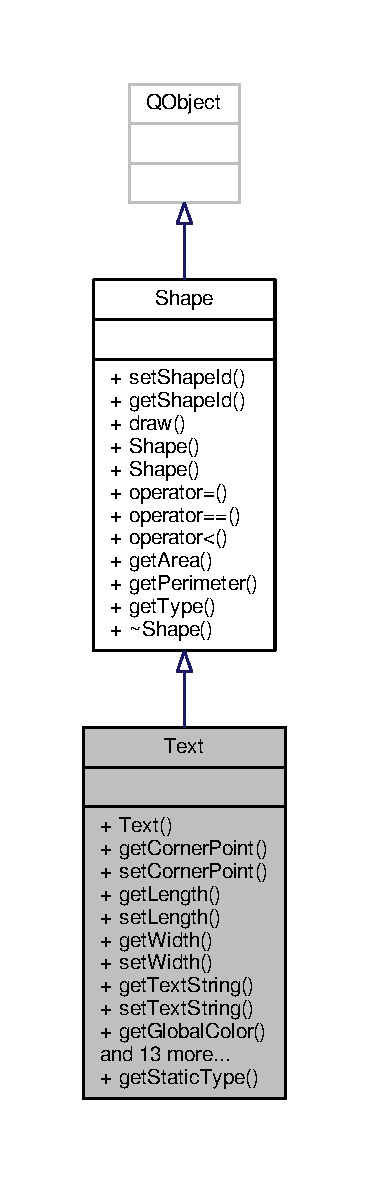
\includegraphics[height=550pt]{classText__inherit__graph}
\end{center}
\end{figure}


Collaboration diagram for Text\+:\nopagebreak
\begin{figure}[H]
\begin{center}
\leavevmode
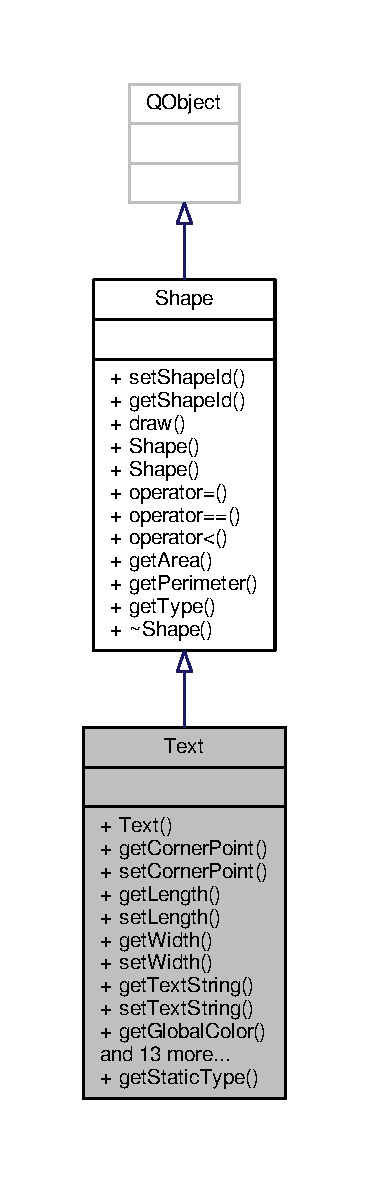
\includegraphics[height=550pt]{classText__coll__graph}
\end{center}
\end{figure}
\subsection*{Public Member Functions}
\begin{DoxyCompactItemize}
\item 
\hyperlink{classText_a2af2490841998a368bccb3eaed6d3698}{Text} (unsigned int, int, int, int, int, Q\+String, Qt\+::\+Global\+Color, Qt\+::\+Alignment\+Flag, int, Q\+String, Q\+Font\+::\+Style, Q\+Font\+::\+Weight)
\begin{DoxyCompactList}\small\item\em \hyperlink{classText}{Text} all parameter constructor. \end{DoxyCompactList}\item 
Q\+Point \hyperlink{classText_a599aa1ac67ad501551a851f2dbc1d90a}{get\+Corner\+Point} ()
\begin{DoxyCompactList}\small\item\em Gets the top left corner of the text drawing rectangle. \end{DoxyCompactList}\item 
void \hyperlink{classText_a8a8424a8e6386a0626cba6ddfa1a91c2}{set\+Corner\+Point} (Q\+Point p1)
\begin{DoxyCompactList}\small\item\em Sets the top left corner of the text drawing rectangle to the given Q\+Point. \end{DoxyCompactList}\item 
int \hyperlink{classText_a0d184f40401d7b4a8127470702bbe1ea}{get\+Length} ()
\begin{DoxyCompactList}\small\item\em Gets the length of the text drawing rectangle. \end{DoxyCompactList}\item 
void \hyperlink{classText_af833cfc1f38ddd0021ac7d1c65f0acb9}{set\+Length} (int \hyperlink{shape__input__file__specs_8txt_a2e02238fe11bc76d2a69c565c7391545}{l})
\begin{DoxyCompactList}\small\item\em Sets the length of the drawing rectangle. \end{DoxyCompactList}\item 
int \hyperlink{classText_aa426e679627149ff986a2c793b2ac71d}{get\+Width} ()
\begin{DoxyCompactList}\small\item\em Gets the width of the drawing rectangle. \end{DoxyCompactList}\item 
void \hyperlink{classText_adb7d8d7de01f5ee0d4de99092e728db6}{set\+Width} (int w)
\begin{DoxyCompactList}\small\item\em Sets the width of the drawing rectangle to the given width. \end{DoxyCompactList}\item 
Q\+String \hyperlink{classText_a873c6803659cfbc8282f746d6a15f158}{get\+Text\+String} ()
\begin{DoxyCompactList}\small\item\em Gets the string of text that is to be drawn. \end{DoxyCompactList}\item 
void \hyperlink{classText_a84348cf4792c9c9b31c50db0ff776784}{set\+Text\+String} (Q\+String ts)
\begin{DoxyCompactList}\small\item\em Sets the string of text to be drawn. \end{DoxyCompactList}\item 
Qt\+::\+Global\+Color \hyperlink{classText_ac6681a7e36595ab4465814caf87418e1}{get\+Global\+Color} ()
\begin{DoxyCompactList}\small\item\em Gets the color of the text. \end{DoxyCompactList}\item 
void \hyperlink{classText_afd3587da630468e7b7c78b4160cb2837}{set\+Global\+Color} (Qt\+::\+Global\+Color gc)
\begin{DoxyCompactList}\small\item\em Sets the color of the text. \end{DoxyCompactList}\item 
Qt\+::\+Alignment\+Flag \hyperlink{classText_a20c87e3d4ca218bdaae3181922091ca5}{get\+Alignment\+Flag} ()
\begin{DoxyCompactList}\small\item\em Gets the alignment flag of the text. \end{DoxyCompactList}\item 
void \hyperlink{classText_a7eddf71ff09b1b20499d2a05ac017dd7}{set\+Alignment\+Flag} (Qt\+::\+Alignment\+Flag af)
\begin{DoxyCompactList}\small\item\em Sets the Alignment of the text. \end{DoxyCompactList}\item 
int \hyperlink{classText_a14d8585dd9a39a1bfecd1b2b44131464}{get\+Text\+Point\+Size} ()
\begin{DoxyCompactList}\small\item\em Gets the point size of the text. \end{DoxyCompactList}\item 
void \hyperlink{classText_ad1e9aabbb6fc0aebc94b3855e32eea78}{set\+Text\+Point\+Size} (int ts)
\begin{DoxyCompactList}\small\item\em Sets the point size to the given point size. \end{DoxyCompactList}\item 
Q\+String \hyperlink{classText_ac72f905a25316d1c271674811e31f724}{get\+Text\+Font\+Family} ()
\begin{DoxyCompactList}\small\item\em Gets the font family of the text. \end{DoxyCompactList}\item 
void \hyperlink{classText_addb9d731d7822aa2d5956d9dc0201500}{set\+Text\+Font\+Family} (Q\+String tff)
\begin{DoxyCompactList}\small\item\em Sets the font family of the text to the given font family. \end{DoxyCompactList}\item 
Q\+Font\+::\+Style \hyperlink{classText_ad572034a19f008c64c63e858cf02a0a4}{get\+Text\+Font\+Style} ()
\begin{DoxyCompactList}\small\item\em Gets the Font Style of the text. \end{DoxyCompactList}\item 
void \hyperlink{classText_acd45f77b52ddeeeeec895fb06997784f}{set\+Text\+Font\+Style} (Q\+Font\+::\+Style tfs)
\begin{DoxyCompactList}\small\item\em Sets the font style of the text to the given font style. \end{DoxyCompactList}\item 
Q\+Font\+::\+Weight \hyperlink{classText_a633a61b274b66c47244430638cd57233}{get\+Text\+Font\+Weight} ()
\begin{DoxyCompactList}\small\item\em Gets the Font Weight of the text. \end{DoxyCompactList}\item 
void \hyperlink{classText_afc544d4b1e989b7386026c39f9413228}{set\+Text\+Font\+Weight} (Q\+Font\+::\+Weight tfw)
\begin{DoxyCompactList}\small\item\em Sets the Font Weight of the text to the given Font Weight. \end{DoxyCompactList}\item 
virtual void \hyperlink{classText_a54e8085e0b04abba6b4a09232ff21449}{draw} (Q\+Painter \&, bool)
\begin{DoxyCompactList}\small\item\em Virtual function to draw shapes. \end{DoxyCompactList}\item 
virtual int \hyperlink{classText_a701eda01498e972823f4c833ed0e8811}{get\+Type} ()
\begin{DoxyCompactList}\small\item\em Gets the type of the shape. \end{DoxyCompactList}\end{DoxyCompactItemize}
\subsection*{Static Public Member Functions}
\begin{DoxyCompactItemize}
\item 
static int \hyperlink{classText_aa63f66168dc6f0af547710743a52f9c9}{get\+Static\+Type} ()
\begin{DoxyCompactList}\small\item\em gets the Type of object \end{DoxyCompactList}\end{DoxyCompactItemize}


\subsection{Detailed Description}
\hyperlink{classText}{Text} class that Q\+Painter can draw. 

\subsection{Constructor \& Destructor Documentation}
\index{Text@{Text}!Text@{Text}}
\index{Text@{Text}!Text@{Text}}
\subsubsection[{\texorpdfstring{Text(unsigned int, int, int, int, int, Q\+String, Qt\+::\+Global\+Color, Qt\+::\+Alignment\+Flag, int, Q\+String, Q\+Font\+::\+Style, Q\+Font\+::\+Weight)}{Text(unsigned int, int, int, int, int, QString, Qt::GlobalColor, Qt::AlignmentFlag, int, QString, QFont::Style, QFont::Weight)}}]{\setlength{\rightskip}{0pt plus 5cm}Text\+::\+Text (
\begin{DoxyParamCaption}
\item[{unsigned int}]{i, }
\item[{int}]{x, }
\item[{int}]{y, }
\item[{int}]{l, }
\item[{int}]{w, }
\item[{Q\+String}]{txt, }
\item[{Qt\+::\+Global\+Color}]{tc, }
\item[{Qt\+::\+Alignment\+Flag}]{ta, }
\item[{int}]{tps, }
\item[{Q\+String}]{tff, }
\item[{Q\+Font\+::\+Style}]{tfs, }
\item[{Q\+Font\+::\+Weight}]{tfw}
\end{DoxyParamCaption}
)}\hypertarget{classText_a2af2490841998a368bccb3eaed6d3698}{}\label{classText_a2af2490841998a368bccb3eaed6d3698}


\hyperlink{classText}{Text} all parameter constructor. 



\subsection{Member Function Documentation}
\index{Text@{Text}!draw@{draw}}
\index{draw@{draw}!Text@{Text}}
\subsubsection[{\texorpdfstring{draw(\+Q\+Painter \&, bool)}{draw(QPainter &, bool)}}]{\setlength{\rightskip}{0pt plus 5cm}void Text\+::draw (
\begin{DoxyParamCaption}
\item[{Q\+Painter \&}]{, }
\item[{bool}]{}
\end{DoxyParamCaption}
)\hspace{0.3cm}{\ttfamily [virtual]}}\hypertarget{classText_a54e8085e0b04abba6b4a09232ff21449}{}\label{classText_a54e8085e0b04abba6b4a09232ff21449}


Virtual function to draw shapes. 



Implements \hyperlink{classShape_a47dae32819e64fb32f3357f31978293f}{Shape}.

\index{Text@{Text}!get\+Alignment\+Flag@{get\+Alignment\+Flag}}
\index{get\+Alignment\+Flag@{get\+Alignment\+Flag}!Text@{Text}}
\subsubsection[{\texorpdfstring{get\+Alignment\+Flag()}{getAlignmentFlag()}}]{\setlength{\rightskip}{0pt plus 5cm}Qt\+::\+Alignment\+Flag Text\+::get\+Alignment\+Flag (
\begin{DoxyParamCaption}
{}
\end{DoxyParamCaption}
)\hspace{0.3cm}{\ttfamily [inline]}}\hypertarget{classText_a20c87e3d4ca218bdaae3181922091ca5}{}\label{classText_a20c87e3d4ca218bdaae3181922091ca5}


Gets the alignment flag of the text. 

\begin{DoxyReturn}{Returns}
Qt\+::\+Alignment\+Flag alignment of text 
\end{DoxyReturn}
\index{Text@{Text}!get\+Corner\+Point@{get\+Corner\+Point}}
\index{get\+Corner\+Point@{get\+Corner\+Point}!Text@{Text}}
\subsubsection[{\texorpdfstring{get\+Corner\+Point()}{getCornerPoint()}}]{\setlength{\rightskip}{0pt plus 5cm}Q\+Point Text\+::get\+Corner\+Point (
\begin{DoxyParamCaption}
{}
\end{DoxyParamCaption}
)\hspace{0.3cm}{\ttfamily [inline]}}\hypertarget{classText_a599aa1ac67ad501551a851f2dbc1d90a}{}\label{classText_a599aa1ac67ad501551a851f2dbc1d90a}


Gets the top left corner of the text drawing rectangle. 

\begin{DoxyReturn}{Returns}
Q\+Point top left corner 
\end{DoxyReturn}
\index{Text@{Text}!get\+Global\+Color@{get\+Global\+Color}}
\index{get\+Global\+Color@{get\+Global\+Color}!Text@{Text}}
\subsubsection[{\texorpdfstring{get\+Global\+Color()}{getGlobalColor()}}]{\setlength{\rightskip}{0pt plus 5cm}Qt\+::\+Global\+Color Text\+::get\+Global\+Color (
\begin{DoxyParamCaption}
{}
\end{DoxyParamCaption}
)\hspace{0.3cm}{\ttfamily [inline]}}\hypertarget{classText_ac6681a7e36595ab4465814caf87418e1}{}\label{classText_ac6681a7e36595ab4465814caf87418e1}


Gets the color of the text. 

\begin{DoxyReturn}{Returns}
Qt\+::\+Global\+Color text color 
\end{DoxyReturn}
\index{Text@{Text}!get\+Length@{get\+Length}}
\index{get\+Length@{get\+Length}!Text@{Text}}
\subsubsection[{\texorpdfstring{get\+Length()}{getLength()}}]{\setlength{\rightskip}{0pt plus 5cm}int Text\+::get\+Length (
\begin{DoxyParamCaption}
{}
\end{DoxyParamCaption}
)\hspace{0.3cm}{\ttfamily [inline]}}\hypertarget{classText_a0d184f40401d7b4a8127470702bbe1ea}{}\label{classText_a0d184f40401d7b4a8127470702bbe1ea}


Gets the length of the text drawing rectangle. 

\begin{DoxyReturn}{Returns}
int length 
\end{DoxyReturn}
\index{Text@{Text}!get\+Static\+Type@{get\+Static\+Type}}
\index{get\+Static\+Type@{get\+Static\+Type}!Text@{Text}}
\subsubsection[{\texorpdfstring{get\+Static\+Type()}{getStaticType()}}]{\setlength{\rightskip}{0pt plus 5cm}static int Text\+::get\+Static\+Type (
\begin{DoxyParamCaption}
{}
\end{DoxyParamCaption}
)\hspace{0.3cm}{\ttfamily [inline]}, {\ttfamily [static]}}\hypertarget{classText_aa63f66168dc6f0af547710743a52f9c9}{}\label{classText_aa63f66168dc6f0af547710743a52f9c9}


gets the Type of object 

\begin{DoxyReturn}{Returns}
Type as int 
\end{DoxyReturn}
\index{Text@{Text}!get\+Text\+Font\+Family@{get\+Text\+Font\+Family}}
\index{get\+Text\+Font\+Family@{get\+Text\+Font\+Family}!Text@{Text}}
\subsubsection[{\texorpdfstring{get\+Text\+Font\+Family()}{getTextFontFamily()}}]{\setlength{\rightskip}{0pt plus 5cm}Q\+String Text\+::get\+Text\+Font\+Family (
\begin{DoxyParamCaption}
{}
\end{DoxyParamCaption}
)\hspace{0.3cm}{\ttfamily [inline]}}\hypertarget{classText_ac72f905a25316d1c271674811e31f724}{}\label{classText_ac72f905a25316d1c271674811e31f724}


Gets the font family of the text. 

\begin{DoxyReturn}{Returns}
Q\+String text font family 
\end{DoxyReturn}
\index{Text@{Text}!get\+Text\+Font\+Style@{get\+Text\+Font\+Style}}
\index{get\+Text\+Font\+Style@{get\+Text\+Font\+Style}!Text@{Text}}
\subsubsection[{\texorpdfstring{get\+Text\+Font\+Style()}{getTextFontStyle()}}]{\setlength{\rightskip}{0pt plus 5cm}Q\+Font\+::\+Style Text\+::get\+Text\+Font\+Style (
\begin{DoxyParamCaption}
{}
\end{DoxyParamCaption}
)\hspace{0.3cm}{\ttfamily [inline]}}\hypertarget{classText_ad572034a19f008c64c63e858cf02a0a4}{}\label{classText_ad572034a19f008c64c63e858cf02a0a4}


Gets the Font Style of the text. 

\begin{DoxyReturn}{Returns}
Q\+Font\+::\+Style 
\end{DoxyReturn}
\index{Text@{Text}!get\+Text\+Font\+Weight@{get\+Text\+Font\+Weight}}
\index{get\+Text\+Font\+Weight@{get\+Text\+Font\+Weight}!Text@{Text}}
\subsubsection[{\texorpdfstring{get\+Text\+Font\+Weight()}{getTextFontWeight()}}]{\setlength{\rightskip}{0pt plus 5cm}Q\+Font\+::\+Weight Text\+::get\+Text\+Font\+Weight (
\begin{DoxyParamCaption}
{}
\end{DoxyParamCaption}
)\hspace{0.3cm}{\ttfamily [inline]}}\hypertarget{classText_a633a61b274b66c47244430638cd57233}{}\label{classText_a633a61b274b66c47244430638cd57233}


Gets the Font Weight of the text. 

\begin{DoxyReturn}{Returns}
Q\+Font\+::\+Weight 
\end{DoxyReturn}
\index{Text@{Text}!get\+Text\+Point\+Size@{get\+Text\+Point\+Size}}
\index{get\+Text\+Point\+Size@{get\+Text\+Point\+Size}!Text@{Text}}
\subsubsection[{\texorpdfstring{get\+Text\+Point\+Size()}{getTextPointSize()}}]{\setlength{\rightskip}{0pt plus 5cm}int Text\+::get\+Text\+Point\+Size (
\begin{DoxyParamCaption}
{}
\end{DoxyParamCaption}
)\hspace{0.3cm}{\ttfamily [inline]}}\hypertarget{classText_a14d8585dd9a39a1bfecd1b2b44131464}{}\label{classText_a14d8585dd9a39a1bfecd1b2b44131464}


Gets the point size of the text. 

\begin{DoxyReturn}{Returns}
int point\+Size 
\end{DoxyReturn}
\index{Text@{Text}!get\+Text\+String@{get\+Text\+String}}
\index{get\+Text\+String@{get\+Text\+String}!Text@{Text}}
\subsubsection[{\texorpdfstring{get\+Text\+String()}{getTextString()}}]{\setlength{\rightskip}{0pt plus 5cm}Q\+String Text\+::get\+Text\+String (
\begin{DoxyParamCaption}
{}
\end{DoxyParamCaption}
)\hspace{0.3cm}{\ttfamily [inline]}}\hypertarget{classText_a873c6803659cfbc8282f746d6a15f158}{}\label{classText_a873c6803659cfbc8282f746d6a15f158}


Gets the string of text that is to be drawn. 

\begin{DoxyReturn}{Returns}
Q\+String text\+String 
\end{DoxyReturn}
\index{Text@{Text}!get\+Type@{get\+Type}}
\index{get\+Type@{get\+Type}!Text@{Text}}
\subsubsection[{\texorpdfstring{get\+Type()}{getType()}}]{\setlength{\rightskip}{0pt plus 5cm}virtual int Text\+::get\+Type (
\begin{DoxyParamCaption}
{}
\end{DoxyParamCaption}
)\hspace{0.3cm}{\ttfamily [inline]}, {\ttfamily [virtual]}}\hypertarget{classText_a701eda01498e972823f4c833ed0e8811}{}\label{classText_a701eda01498e972823f4c833ed0e8811}


Gets the type of the shape. 

\begin{DoxyReturn}{Returns}
type as an int 
\end{DoxyReturn}


Implements \hyperlink{classShape_a3d15adf2a1d746928f9be98105096eda}{Shape}.

\index{Text@{Text}!get\+Width@{get\+Width}}
\index{get\+Width@{get\+Width}!Text@{Text}}
\subsubsection[{\texorpdfstring{get\+Width()}{getWidth()}}]{\setlength{\rightskip}{0pt plus 5cm}int Text\+::get\+Width (
\begin{DoxyParamCaption}
{}
\end{DoxyParamCaption}
)\hspace{0.3cm}{\ttfamily [inline]}}\hypertarget{classText_aa426e679627149ff986a2c793b2ac71d}{}\label{classText_aa426e679627149ff986a2c793b2ac71d}


Gets the width of the drawing rectangle. 

\begin{DoxyReturn}{Returns}
int width of rectangle 
\end{DoxyReturn}
\index{Text@{Text}!set\+Alignment\+Flag@{set\+Alignment\+Flag}}
\index{set\+Alignment\+Flag@{set\+Alignment\+Flag}!Text@{Text}}
\subsubsection[{\texorpdfstring{set\+Alignment\+Flag(\+Qt\+::\+Alignment\+Flag af)}{setAlignmentFlag(Qt::AlignmentFlag af)}}]{\setlength{\rightskip}{0pt plus 5cm}void Text\+::set\+Alignment\+Flag (
\begin{DoxyParamCaption}
\item[{Qt\+::\+Alignment\+Flag}]{af}
\end{DoxyParamCaption}
)\hspace{0.3cm}{\ttfamily [inline]}}\hypertarget{classText_a7eddf71ff09b1b20499d2a05ac017dd7}{}\label{classText_a7eddf71ff09b1b20499d2a05ac017dd7}


Sets the Alignment of the text. 


\begin{DoxyParams}{Parameters}
{\em af} & Qt\+::\+A\+Lignment\+Flag \\
\hline
\end{DoxyParams}
\index{Text@{Text}!set\+Corner\+Point@{set\+Corner\+Point}}
\index{set\+Corner\+Point@{set\+Corner\+Point}!Text@{Text}}
\subsubsection[{\texorpdfstring{set\+Corner\+Point(\+Q\+Point p1)}{setCornerPoint(QPoint p1)}}]{\setlength{\rightskip}{0pt plus 5cm}void Text\+::set\+Corner\+Point (
\begin{DoxyParamCaption}
\item[{Q\+Point}]{p1}
\end{DoxyParamCaption}
)\hspace{0.3cm}{\ttfamily [inline]}}\hypertarget{classText_a8a8424a8e6386a0626cba6ddfa1a91c2}{}\label{classText_a8a8424a8e6386a0626cba6ddfa1a91c2}


Sets the top left corner of the text drawing rectangle to the given Q\+Point. 


\begin{DoxyParams}{Parameters}
{\em p1} & Q\+Point \\
\hline
\end{DoxyParams}
\index{Text@{Text}!set\+Global\+Color@{set\+Global\+Color}}
\index{set\+Global\+Color@{set\+Global\+Color}!Text@{Text}}
\subsubsection[{\texorpdfstring{set\+Global\+Color(\+Qt\+::\+Global\+Color gc)}{setGlobalColor(Qt::GlobalColor gc)}}]{\setlength{\rightskip}{0pt plus 5cm}void Text\+::set\+Global\+Color (
\begin{DoxyParamCaption}
\item[{Qt\+::\+Global\+Color}]{gc}
\end{DoxyParamCaption}
)\hspace{0.3cm}{\ttfamily [inline]}}\hypertarget{classText_afd3587da630468e7b7c78b4160cb2837}{}\label{classText_afd3587da630468e7b7c78b4160cb2837}


Sets the color of the text. 


\begin{DoxyParams}{Parameters}
{\em gc} & Qt\+::\+Global\+Color for the text color \\
\hline
\end{DoxyParams}
\index{Text@{Text}!set\+Length@{set\+Length}}
\index{set\+Length@{set\+Length}!Text@{Text}}
\subsubsection[{\texorpdfstring{set\+Length(int l)}{setLength(int l)}}]{\setlength{\rightskip}{0pt plus 5cm}void Text\+::set\+Length (
\begin{DoxyParamCaption}
\item[{int}]{l}
\end{DoxyParamCaption}
)\hspace{0.3cm}{\ttfamily [inline]}}\hypertarget{classText_af833cfc1f38ddd0021ac7d1c65f0acb9}{}\label{classText_af833cfc1f38ddd0021ac7d1c65f0acb9}


Sets the length of the drawing rectangle. 


\begin{DoxyParams}{Parameters}
{\em l} & length of drawing rectangle \\
\hline
\end{DoxyParams}
\index{Text@{Text}!set\+Text\+Font\+Family@{set\+Text\+Font\+Family}}
\index{set\+Text\+Font\+Family@{set\+Text\+Font\+Family}!Text@{Text}}
\subsubsection[{\texorpdfstring{set\+Text\+Font\+Family(\+Q\+String tff)}{setTextFontFamily(QString tff)}}]{\setlength{\rightskip}{0pt plus 5cm}void Text\+::set\+Text\+Font\+Family (
\begin{DoxyParamCaption}
\item[{Q\+String}]{tff}
\end{DoxyParamCaption}
)\hspace{0.3cm}{\ttfamily [inline]}}\hypertarget{classText_addb9d731d7822aa2d5956d9dc0201500}{}\label{classText_addb9d731d7822aa2d5956d9dc0201500}


Sets the font family of the text to the given font family. 


\begin{DoxyParams}{Parameters}
{\em tff} & Q\+String of the font family \\
\hline
\end{DoxyParams}
\index{Text@{Text}!set\+Text\+Font\+Style@{set\+Text\+Font\+Style}}
\index{set\+Text\+Font\+Style@{set\+Text\+Font\+Style}!Text@{Text}}
\subsubsection[{\texorpdfstring{set\+Text\+Font\+Style(\+Q\+Font\+::\+Style tfs)}{setTextFontStyle(QFont::Style tfs)}}]{\setlength{\rightskip}{0pt plus 5cm}void Text\+::set\+Text\+Font\+Style (
\begin{DoxyParamCaption}
\item[{Q\+Font\+::\+Style}]{tfs}
\end{DoxyParamCaption}
)\hspace{0.3cm}{\ttfamily [inline]}}\hypertarget{classText_acd45f77b52ddeeeeec895fb06997784f}{}\label{classText_acd45f77b52ddeeeeec895fb06997784f}


Sets the font style of the text to the given font style. 


\begin{DoxyParams}{Parameters}
{\em tfs} & Q\+Font\+::\+Style \\
\hline
\end{DoxyParams}
\index{Text@{Text}!set\+Text\+Font\+Weight@{set\+Text\+Font\+Weight}}
\index{set\+Text\+Font\+Weight@{set\+Text\+Font\+Weight}!Text@{Text}}
\subsubsection[{\texorpdfstring{set\+Text\+Font\+Weight(\+Q\+Font\+::\+Weight tfw)}{setTextFontWeight(QFont::Weight tfw)}}]{\setlength{\rightskip}{0pt plus 5cm}void Text\+::set\+Text\+Font\+Weight (
\begin{DoxyParamCaption}
\item[{Q\+Font\+::\+Weight}]{tfw}
\end{DoxyParamCaption}
)\hspace{0.3cm}{\ttfamily [inline]}}\hypertarget{classText_afc544d4b1e989b7386026c39f9413228}{}\label{classText_afc544d4b1e989b7386026c39f9413228}


Sets the Font Weight of the text to the given Font Weight. 


\begin{DoxyParams}{Parameters}
{\em tfw} & Q\+Font\+::\+Weight \\
\hline
\end{DoxyParams}
\index{Text@{Text}!set\+Text\+Point\+Size@{set\+Text\+Point\+Size}}
\index{set\+Text\+Point\+Size@{set\+Text\+Point\+Size}!Text@{Text}}
\subsubsection[{\texorpdfstring{set\+Text\+Point\+Size(int ts)}{setTextPointSize(int ts)}}]{\setlength{\rightskip}{0pt plus 5cm}void Text\+::set\+Text\+Point\+Size (
\begin{DoxyParamCaption}
\item[{int}]{ts}
\end{DoxyParamCaption}
)\hspace{0.3cm}{\ttfamily [inline]}}\hypertarget{classText_ad1e9aabbb6fc0aebc94b3855e32eea78}{}\label{classText_ad1e9aabbb6fc0aebc94b3855e32eea78}


Sets the point size to the given point size. 


\begin{DoxyParams}{Parameters}
{\em ts} & int Point size \\
\hline
\end{DoxyParams}
\index{Text@{Text}!set\+Text\+String@{set\+Text\+String}}
\index{set\+Text\+String@{set\+Text\+String}!Text@{Text}}
\subsubsection[{\texorpdfstring{set\+Text\+String(\+Q\+String ts)}{setTextString(QString ts)}}]{\setlength{\rightskip}{0pt plus 5cm}void Text\+::set\+Text\+String (
\begin{DoxyParamCaption}
\item[{Q\+String}]{ts}
\end{DoxyParamCaption}
)\hspace{0.3cm}{\ttfamily [inline]}}\hypertarget{classText_a84348cf4792c9c9b31c50db0ff776784}{}\label{classText_a84348cf4792c9c9b31c50db0ff776784}


Sets the string of text to be drawn. 


\begin{DoxyParams}{Parameters}
{\em ts} & Q\+String of the text \\
\hline
\end{DoxyParams}
\index{Text@{Text}!set\+Width@{set\+Width}}
\index{set\+Width@{set\+Width}!Text@{Text}}
\subsubsection[{\texorpdfstring{set\+Width(int w)}{setWidth(int w)}}]{\setlength{\rightskip}{0pt plus 5cm}void Text\+::set\+Width (
\begin{DoxyParamCaption}
\item[{int}]{w}
\end{DoxyParamCaption}
)\hspace{0.3cm}{\ttfamily [inline]}}\hypertarget{classText_adb7d8d7de01f5ee0d4de99092e728db6}{}\label{classText_adb7d8d7de01f5ee0d4de99092e728db6}


Sets the width of the drawing rectangle to the given width. 


\begin{DoxyParams}{Parameters}
{\em w} & width of drawing rectangle \\
\hline
\end{DoxyParams}


The documentation for this class was generated from the following files\+:\begin{DoxyCompactItemize}
\item 
Group Project/\+Scrum\+Of\+The\+Earth/\hyperlink{text_8h}{text.\+h}\item 
Group Project/\+Scrum\+Of\+The\+Earth/\hyperlink{text_8cpp}{text.\+cpp}\end{DoxyCompactItemize}

\hypertarget{classmyStd_1_1vector}{}\section{my\+Std\+:\+:vector$<$ T $>$ Class Template Reference}
\label{classmyStd_1_1vector}\index{my\+Std\+::vector$<$ T $>$@{my\+Std\+::vector$<$ T $>$}}


The vector class provides a templated dynamic array for use.  




{\ttfamily \#include $<$vector.\+h$>$}



Collaboration diagram for my\+Std\+:\+:vector$<$ T $>$\+:
\nopagebreak
\begin{figure}[H]
\begin{center}
\leavevmode
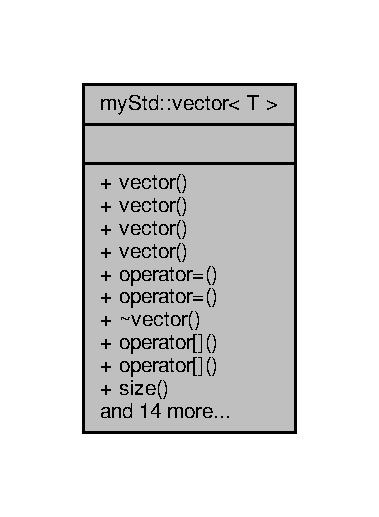
\includegraphics[width=182pt]{classmyStd_1_1vector__coll__graph}
\end{center}
\end{figure}
\subsection*{Public Types}
\begin{DoxyCompactItemize}
\item 
using \hyperlink{classmyStd_1_1vector_a667a65b093f1253d2229d06768aa3bf9}{iterator} = T $\ast$
\item 
using \hyperlink{classmyStd_1_1vector_ae8f53b1db01169b861f0299f9ced0e37}{const\+\_\+iterator} = const T $\ast$
\end{DoxyCompactItemize}
\subsection*{Public Member Functions}
\begin{DoxyCompactItemize}
\item 
\hyperlink{classmyStd_1_1vector_a40e5c01ceb5d0c2bc64b23005c21ba04}{vector} ()
\begin{DoxyCompactList}\small\item\em vector default constructor \end{DoxyCompactList}\item 
\hyperlink{classmyStd_1_1vector_a3f942029ffea510e3c6e67310c18abb7}{vector} (int s)
\begin{DoxyCompactList}\small\item\em vector constructor with size \end{DoxyCompactList}\item 
\hyperlink{classmyStd_1_1vector_ae425fb0a79cfa7870cf3603c8abe3369}{vector} (const \hyperlink{classmyStd_1_1vector}{vector} \&src)
\begin{DoxyCompactList}\small\item\em vector copy constructor \end{DoxyCompactList}\item 
\hyperlink{classmyStd_1_1vector_a76692ca684b66499d2877824e1404205}{vector} (\hyperlink{classmyStd_1_1vector}{vector} \&\&src)
\begin{DoxyCompactList}\small\item\em vector move constructor \end{DoxyCompactList}\item 
\hyperlink{classmyStd_1_1vector}{vector} \& \hyperlink{classmyStd_1_1vector_a5cbbf45fd8ead8b9cbf4b0c7acf5010f}{operator=} (const \hyperlink{classmyStd_1_1vector}{vector} \&src)
\begin{DoxyCompactList}\small\item\em operator = copy assignment \end{DoxyCompactList}\item 
\hyperlink{classmyStd_1_1vector}{vector} \& \hyperlink{classmyStd_1_1vector_a8aac18132c15abb44dea31300923ef3f}{operator=} (\hyperlink{classmyStd_1_1vector}{vector} \&\&src)
\begin{DoxyCompactList}\small\item\em operator = move assignment \end{DoxyCompactList}\item 
\hyperlink{classmyStd_1_1vector_aaf4331a544887b4358befcfbce2deab4}{$\sim$vector} ()
\begin{DoxyCompactList}\small\item\em Vector destructor (Does not delete pointed to data) \end{DoxyCompactList}\item 
T \& \hyperlink{classmyStd_1_1vector_a7840f76cb8fdb56e3a70506c7e0fbf5a}{operator\mbox{[}$\,$\mbox{]}} (int n)
\begin{DoxyCompactList}\small\item\em operator \mbox{[}\mbox{]} gets the element at the n-\/th position by reference \end{DoxyCompactList}\item 
const T \& \hyperlink{classmyStd_1_1vector_ac86fa3944b7d23fc127f5b739935b5d6}{operator\mbox{[}$\,$\mbox{]}} (int n) const 
\begin{DoxyCompactList}\small\item\em operator \mbox{[}\mbox{]} gets the element at the n-\/th position by value \end{DoxyCompactList}\item 
int \hyperlink{classmyStd_1_1vector_a33ebe4dab379f466c8d3a2f08d9aa554}{size} () const 
\begin{DoxyCompactList}\small\item\em size gets the number of elements in the vector \end{DoxyCompactList}\item 
int \hyperlink{classmyStd_1_1vector_ad388bb612c6b9945731d562aeae8695b}{capacity} () const 
\begin{DoxyCompactList}\small\item\em capacity Amount of elements that can be stored in vector \end{DoxyCompactList}\item 
void \hyperlink{classmyStd_1_1vector_aa54bd9c3d8d3b6191d7eb7f85490eadb}{resize} (int newsize)
\begin{DoxyCompactList}\small\item\em resize changes the size of the vector to the specified size \end{DoxyCompactList}\item 
void \hyperlink{classmyStd_1_1vector_a16a7791abc12b34fee94f4ef48a5e157}{push\+\_\+back} (T d)
\begin{DoxyCompactList}\small\item\em push\+\_\+back adds an element to the end of the vector \end{DoxyCompactList}\item 
void \hyperlink{classmyStd_1_1vector_a50e786a02a59e689999365037ae26b3a}{reserve} (int newalloc)
\begin{DoxyCompactList}\small\item\em reserve sets aside a new vector of the given size \end{DoxyCompactList}\item 
\hyperlink{classmyStd_1_1vector_a667a65b093f1253d2229d06768aa3bf9}{iterator} \hyperlink{classmyStd_1_1vector_adaa284b6b387f70d3244b4d6e64869c3}{begin} ()
\begin{DoxyCompactList}\small\item\em begin returns an iterator of the beginning of the vector \end{DoxyCompactList}\item 
\hyperlink{classmyStd_1_1vector_ae8f53b1db01169b861f0299f9ced0e37}{const\+\_\+iterator} \hyperlink{classmyStd_1_1vector_a71600f2a06ab5c279a469972d713d5d6}{begin} () const 
\begin{DoxyCompactList}\small\item\em begin returns a const\+\_\+iterator to the first element \end{DoxyCompactList}\item 
\hyperlink{classmyStd_1_1vector_a667a65b093f1253d2229d06768aa3bf9}{iterator} \hyperlink{classmyStd_1_1vector_a8fc7ec068c194f5ecb5a08e17a9c9ac4}{end} ()
\begin{DoxyCompactList}\small\item\em end returns an iterator to one past the last element \end{DoxyCompactList}\item 
\hyperlink{classmyStd_1_1vector_ae8f53b1db01169b861f0299f9ced0e37}{const\+\_\+iterator} \hyperlink{classmyStd_1_1vector_adecc27953fecd9a02c54f2b2d6a28cff}{end} () const 
\begin{DoxyCompactList}\small\item\em end returns a const\+\_\+iterator to one past the last element \end{DoxyCompactList}\item 
\hyperlink{classmyStd_1_1vector_a667a65b093f1253d2229d06768aa3bf9}{iterator} \hyperlink{classmyStd_1_1vector_a2dfafafc64febfbb0869be81f6bd4de7}{insert} (\hyperlink{classmyStd_1_1vector_a667a65b093f1253d2229d06768aa3bf9}{iterator} p, const T \&val)
\begin{DoxyCompactList}\small\item\em insert inserts a given value before the position p \end{DoxyCompactList}\item 
\hyperlink{classmyStd_1_1vector_a667a65b093f1253d2229d06768aa3bf9}{iterator} \hyperlink{classmyStd_1_1vector_aa4ecb71647140e3c5226299f84828984}{erase} (\hyperlink{classmyStd_1_1vector_a667a65b093f1253d2229d06768aa3bf9}{iterator} p)
\begin{DoxyCompactList}\small\item\em erase takes out the element at position p \end{DoxyCompactList}\item 
void \hyperlink{classmyStd_1_1vector_a67598296046328471d19ce1fc5be796f}{dealloc\+Ptr\+Data} ()
\begin{DoxyCompactList}\small\item\em dealloc\+Ptr\+Data deallocates all of the pointer data of the vector if the vector is a vector of pointers \end{DoxyCompactList}\item 
void \hyperlink{classmyStd_1_1vector_ab67c727d73d08372770562b4e4ae7a05}{dealloc\+Ptr\+Array\+Data} ()
\begin{DoxyCompactList}\small\item\em dealloc\+Ptr\+Array\+Data dellocates all pointed to arrays of the vector if the vector is a vector of dynamic arrays \end{DoxyCompactList}\item 
void \hyperlink{classmyStd_1_1vector_a794565e7ec67e8d2b90fe2247612a778}{delete\+List} ()
\begin{DoxyCompactList}\small\item\em delete\+List deletes the whole vector of pointed to data \end{DoxyCompactList}\item 
void \hyperlink{classmyStd_1_1vector_a6a0db76b04cb2c2bf8b7aa9d2a6f36c4}{delete\+Array\+List} ()
\begin{DoxyCompactList}\small\item\em delete\+Array\+List deletes the whole vector of pointed to arrays \end{DoxyCompactList}\end{DoxyCompactItemize}


\subsection{Detailed Description}
\subsubsection*{template$<$typename T$>$\\*
class my\+Std\+::vector$<$ T $>$}

The vector class provides a templated dynamic array for use. 

\subsection{Member Typedef Documentation}
\index{my\+Std\+::vector@{my\+Std\+::vector}!const\+\_\+iterator@{const\+\_\+iterator}}
\index{const\+\_\+iterator@{const\+\_\+iterator}!my\+Std\+::vector@{my\+Std\+::vector}}
\subsubsection[{\texorpdfstring{const\+\_\+iterator}{const_iterator}}]{\setlength{\rightskip}{0pt plus 5cm}template$<$typename T$>$ using {\bf my\+Std\+::vector}$<$ T $>$\+::{\bf const\+\_\+iterator} =  const T $\ast$}\hypertarget{classmyStd_1_1vector_ae8f53b1db01169b861f0299f9ced0e37}{}\label{classmyStd_1_1vector_ae8f53b1db01169b861f0299f9ced0e37}
\index{my\+Std\+::vector@{my\+Std\+::vector}!iterator@{iterator}}
\index{iterator@{iterator}!my\+Std\+::vector@{my\+Std\+::vector}}
\subsubsection[{\texorpdfstring{iterator}{iterator}}]{\setlength{\rightskip}{0pt plus 5cm}template$<$typename T$>$ using {\bf my\+Std\+::vector}$<$ T $>$\+::{\bf iterator} =  T $\ast$}\hypertarget{classmyStd_1_1vector_a667a65b093f1253d2229d06768aa3bf9}{}\label{classmyStd_1_1vector_a667a65b093f1253d2229d06768aa3bf9}


\subsection{Constructor \& Destructor Documentation}
\index{my\+Std\+::vector@{my\+Std\+::vector}!vector@{vector}}
\index{vector@{vector}!my\+Std\+::vector@{my\+Std\+::vector}}
\subsubsection[{\texorpdfstring{vector()}{vector()}}]{\setlength{\rightskip}{0pt plus 5cm}template$<$typename T$>$ {\bf my\+Std\+::vector}$<$ T $>$\+::{\bf vector} (
\begin{DoxyParamCaption}
{}
\end{DoxyParamCaption}
)\hspace{0.3cm}{\ttfamily [inline]}}\hypertarget{classmyStd_1_1vector_a40e5c01ceb5d0c2bc64b23005c21ba04}{}\label{classmyStd_1_1vector_a40e5c01ceb5d0c2bc64b23005c21ba04}


vector default constructor 

\index{my\+Std\+::vector@{my\+Std\+::vector}!vector@{vector}}
\index{vector@{vector}!my\+Std\+::vector@{my\+Std\+::vector}}
\subsubsection[{\texorpdfstring{vector(int s)}{vector(int s)}}]{\setlength{\rightskip}{0pt plus 5cm}template$<$typename T$>$ {\bf my\+Std\+::vector}$<$ T $>$\+::{\bf vector} (
\begin{DoxyParamCaption}
\item[{int}]{s}
\end{DoxyParamCaption}
)\hspace{0.3cm}{\ttfamily [inline]}, {\ttfamily [explicit]}}\hypertarget{classmyStd_1_1vector_a3f942029ffea510e3c6e67310c18abb7}{}\label{classmyStd_1_1vector_a3f942029ffea510e3c6e67310c18abb7}


vector constructor with size 


\begin{DoxyParams}{Parameters}
{\em s} & size of vector \\
\hline
\end{DoxyParams}
\index{my\+Std\+::vector@{my\+Std\+::vector}!vector@{vector}}
\index{vector@{vector}!my\+Std\+::vector@{my\+Std\+::vector}}
\subsubsection[{\texorpdfstring{vector(const vector \&src)}{vector(const vector &src)}}]{\setlength{\rightskip}{0pt plus 5cm}template$<$typename T$>$ {\bf my\+Std\+::vector}$<$ T $>$\+::{\bf vector} (
\begin{DoxyParamCaption}
\item[{const {\bf vector}$<$ T $>$ \&}]{src}
\end{DoxyParamCaption}
)\hspace{0.3cm}{\ttfamily [inline]}}\hypertarget{classmyStd_1_1vector_ae425fb0a79cfa7870cf3603c8abe3369}{}\label{classmyStd_1_1vector_ae425fb0a79cfa7870cf3603c8abe3369}


vector copy constructor 


\begin{DoxyParams}{Parameters}
{\em src} & vector to copy \\
\hline
\end{DoxyParams}
\index{my\+Std\+::vector@{my\+Std\+::vector}!vector@{vector}}
\index{vector@{vector}!my\+Std\+::vector@{my\+Std\+::vector}}
\subsubsection[{\texorpdfstring{vector(vector \&\&src)}{vector(vector &&src)}}]{\setlength{\rightskip}{0pt plus 5cm}template$<$typename T$>$ {\bf my\+Std\+::vector}$<$ T $>$\+::{\bf vector} (
\begin{DoxyParamCaption}
\item[{{\bf vector}$<$ T $>$ \&\&}]{src}
\end{DoxyParamCaption}
)\hspace{0.3cm}{\ttfamily [inline]}}\hypertarget{classmyStd_1_1vector_a76692ca684b66499d2877824e1404205}{}\label{classmyStd_1_1vector_a76692ca684b66499d2877824e1404205}


vector move constructor 


\begin{DoxyParams}{Parameters}
{\em src} & vector to steal contents of \\
\hline
\end{DoxyParams}
\index{my\+Std\+::vector@{my\+Std\+::vector}!````~vector@{$\sim$vector}}
\index{````~vector@{$\sim$vector}!my\+Std\+::vector@{my\+Std\+::vector}}
\subsubsection[{\texorpdfstring{$\sim$vector()}{~vector()}}]{\setlength{\rightskip}{0pt plus 5cm}template$<$typename T$>$ {\bf my\+Std\+::vector}$<$ T $>$\+::$\sim${\bf vector} (
\begin{DoxyParamCaption}
{}
\end{DoxyParamCaption}
)\hspace{0.3cm}{\ttfamily [inline]}}\hypertarget{classmyStd_1_1vector_aaf4331a544887b4358befcfbce2deab4}{}\label{classmyStd_1_1vector_aaf4331a544887b4358befcfbce2deab4}


Vector destructor (Does not delete pointed to data) 



\subsection{Member Function Documentation}
\index{my\+Std\+::vector@{my\+Std\+::vector}!begin@{begin}}
\index{begin@{begin}!my\+Std\+::vector@{my\+Std\+::vector}}
\subsubsection[{\texorpdfstring{begin()}{begin()}}]{\setlength{\rightskip}{0pt plus 5cm}template$<$typename T$>$ {\bf iterator} {\bf my\+Std\+::vector}$<$ T $>$\+::begin (
\begin{DoxyParamCaption}
{}
\end{DoxyParamCaption}
)\hspace{0.3cm}{\ttfamily [inline]}}\hypertarget{classmyStd_1_1vector_adaa284b6b387f70d3244b4d6e64869c3}{}\label{classmyStd_1_1vector_adaa284b6b387f70d3244b4d6e64869c3}


begin returns an iterator of the beginning of the vector 

\begin{DoxyReturn}{Returns}
iterator of the beginning 
\end{DoxyReturn}
\index{my\+Std\+::vector@{my\+Std\+::vector}!begin@{begin}}
\index{begin@{begin}!my\+Std\+::vector@{my\+Std\+::vector}}
\subsubsection[{\texorpdfstring{begin() const }{begin() const }}]{\setlength{\rightskip}{0pt plus 5cm}template$<$typename T$>$ {\bf const\+\_\+iterator} {\bf my\+Std\+::vector}$<$ T $>$\+::begin (
\begin{DoxyParamCaption}
{}
\end{DoxyParamCaption}
) const\hspace{0.3cm}{\ttfamily [inline]}}\hypertarget{classmyStd_1_1vector_a71600f2a06ab5c279a469972d713d5d6}{}\label{classmyStd_1_1vector_a71600f2a06ab5c279a469972d713d5d6}


begin returns a const\+\_\+iterator to the first element 

\begin{DoxyReturn}{Returns}
const\+\_\+iterator to first element 
\end{DoxyReturn}
\index{my\+Std\+::vector@{my\+Std\+::vector}!capacity@{capacity}}
\index{capacity@{capacity}!my\+Std\+::vector@{my\+Std\+::vector}}
\subsubsection[{\texorpdfstring{capacity() const }{capacity() const }}]{\setlength{\rightskip}{0pt plus 5cm}template$<$typename T$>$ int {\bf my\+Std\+::vector}$<$ T $>$\+::capacity (
\begin{DoxyParamCaption}
{}
\end{DoxyParamCaption}
) const\hspace{0.3cm}{\ttfamily [inline]}}\hypertarget{classmyStd_1_1vector_ad388bb612c6b9945731d562aeae8695b}{}\label{classmyStd_1_1vector_ad388bb612c6b9945731d562aeae8695b}


capacity Amount of elements that can be stored in vector 

\begin{DoxyReturn}{Returns}
int size of arrays 
\end{DoxyReturn}
\index{my\+Std\+::vector@{my\+Std\+::vector}!dealloc\+Ptr\+Array\+Data@{dealloc\+Ptr\+Array\+Data}}
\index{dealloc\+Ptr\+Array\+Data@{dealloc\+Ptr\+Array\+Data}!my\+Std\+::vector@{my\+Std\+::vector}}
\subsubsection[{\texorpdfstring{dealloc\+Ptr\+Array\+Data()}{deallocPtrArrayData()}}]{\setlength{\rightskip}{0pt plus 5cm}template$<$typename T$>$ void {\bf my\+Std\+::vector}$<$ T $>$\+::dealloc\+Ptr\+Array\+Data (
\begin{DoxyParamCaption}
{}
\end{DoxyParamCaption}
)\hspace{0.3cm}{\ttfamily [inline]}}\hypertarget{classmyStd_1_1vector_ab67c727d73d08372770562b4e4ae7a05}{}\label{classmyStd_1_1vector_ab67c727d73d08372770562b4e4ae7a05}


dealloc\+Ptr\+Array\+Data dellocates all pointed to arrays of the vector if the vector is a vector of dynamic arrays 

\index{my\+Std\+::vector@{my\+Std\+::vector}!dealloc\+Ptr\+Data@{dealloc\+Ptr\+Data}}
\index{dealloc\+Ptr\+Data@{dealloc\+Ptr\+Data}!my\+Std\+::vector@{my\+Std\+::vector}}
\subsubsection[{\texorpdfstring{dealloc\+Ptr\+Data()}{deallocPtrData()}}]{\setlength{\rightskip}{0pt plus 5cm}template$<$typename T$>$ void {\bf my\+Std\+::vector}$<$ T $>$\+::dealloc\+Ptr\+Data (
\begin{DoxyParamCaption}
{}
\end{DoxyParamCaption}
)\hspace{0.3cm}{\ttfamily [inline]}}\hypertarget{classmyStd_1_1vector_a67598296046328471d19ce1fc5be796f}{}\label{classmyStd_1_1vector_a67598296046328471d19ce1fc5be796f}


dealloc\+Ptr\+Data deallocates all of the pointer data of the vector if the vector is a vector of pointers 

\index{my\+Std\+::vector@{my\+Std\+::vector}!delete\+Array\+List@{delete\+Array\+List}}
\index{delete\+Array\+List@{delete\+Array\+List}!my\+Std\+::vector@{my\+Std\+::vector}}
\subsubsection[{\texorpdfstring{delete\+Array\+List()}{deleteArrayList()}}]{\setlength{\rightskip}{0pt plus 5cm}template$<$typename T$>$ void {\bf my\+Std\+::vector}$<$ T $>$\+::delete\+Array\+List (
\begin{DoxyParamCaption}
{}
\end{DoxyParamCaption}
)\hspace{0.3cm}{\ttfamily [inline]}}\hypertarget{classmyStd_1_1vector_a6a0db76b04cb2c2bf8b7aa9d2a6f36c4}{}\label{classmyStd_1_1vector_a6a0db76b04cb2c2bf8b7aa9d2a6f36c4}


delete\+Array\+List deletes the whole vector of pointed to arrays 

\index{my\+Std\+::vector@{my\+Std\+::vector}!delete\+List@{delete\+List}}
\index{delete\+List@{delete\+List}!my\+Std\+::vector@{my\+Std\+::vector}}
\subsubsection[{\texorpdfstring{delete\+List()}{deleteList()}}]{\setlength{\rightskip}{0pt plus 5cm}template$<$typename T$>$ void {\bf my\+Std\+::vector}$<$ T $>$\+::delete\+List (
\begin{DoxyParamCaption}
{}
\end{DoxyParamCaption}
)\hspace{0.3cm}{\ttfamily [inline]}}\hypertarget{classmyStd_1_1vector_a794565e7ec67e8d2b90fe2247612a778}{}\label{classmyStd_1_1vector_a794565e7ec67e8d2b90fe2247612a778}


delete\+List deletes the whole vector of pointed to data 

\index{my\+Std\+::vector@{my\+Std\+::vector}!end@{end}}
\index{end@{end}!my\+Std\+::vector@{my\+Std\+::vector}}
\subsubsection[{\texorpdfstring{end()}{end()}}]{\setlength{\rightskip}{0pt plus 5cm}template$<$typename T$>$ {\bf iterator} {\bf my\+Std\+::vector}$<$ T $>$\+::end (
\begin{DoxyParamCaption}
{}
\end{DoxyParamCaption}
)\hspace{0.3cm}{\ttfamily [inline]}}\hypertarget{classmyStd_1_1vector_a8fc7ec068c194f5ecb5a08e17a9c9ac4}{}\label{classmyStd_1_1vector_a8fc7ec068c194f5ecb5a08e17a9c9ac4}


end returns an iterator to one past the last element 

\begin{DoxyReturn}{Returns}
iterator to one past the last element 
\end{DoxyReturn}
\index{my\+Std\+::vector@{my\+Std\+::vector}!end@{end}}
\index{end@{end}!my\+Std\+::vector@{my\+Std\+::vector}}
\subsubsection[{\texorpdfstring{end() const }{end() const }}]{\setlength{\rightskip}{0pt plus 5cm}template$<$typename T$>$ {\bf const\+\_\+iterator} {\bf my\+Std\+::vector}$<$ T $>$\+::end (
\begin{DoxyParamCaption}
{}
\end{DoxyParamCaption}
) const\hspace{0.3cm}{\ttfamily [inline]}}\hypertarget{classmyStd_1_1vector_adecc27953fecd9a02c54f2b2d6a28cff}{}\label{classmyStd_1_1vector_adecc27953fecd9a02c54f2b2d6a28cff}


end returns a const\+\_\+iterator to one past the last element 

\begin{DoxyReturn}{Returns}
iterator to one past the last element 
\end{DoxyReturn}
\index{my\+Std\+::vector@{my\+Std\+::vector}!erase@{erase}}
\index{erase@{erase}!my\+Std\+::vector@{my\+Std\+::vector}}
\subsubsection[{\texorpdfstring{erase(iterator p)}{erase(iterator p)}}]{\setlength{\rightskip}{0pt plus 5cm}template$<$typename T$>$ {\bf iterator} {\bf my\+Std\+::vector}$<$ T $>$\+::erase (
\begin{DoxyParamCaption}
\item[{{\bf iterator}}]{p}
\end{DoxyParamCaption}
)\hspace{0.3cm}{\ttfamily [inline]}}\hypertarget{classmyStd_1_1vector_aa4ecb71647140e3c5226299f84828984}{}\label{classmyStd_1_1vector_aa4ecb71647140e3c5226299f84828984}


erase takes out the element at position p 


\begin{DoxyParams}{Parameters}
{\em p} & iterator to element at that position \\
\hline
\end{DoxyParams}
\begin{DoxyReturn}{Returns}

\end{DoxyReturn}
\index{my\+Std\+::vector@{my\+Std\+::vector}!insert@{insert}}
\index{insert@{insert}!my\+Std\+::vector@{my\+Std\+::vector}}
\subsubsection[{\texorpdfstring{insert(iterator p, const T \&val)}{insert(iterator p, const T &val)}}]{\setlength{\rightskip}{0pt plus 5cm}template$<$typename T$>$ {\bf iterator} {\bf my\+Std\+::vector}$<$ T $>$\+::insert (
\begin{DoxyParamCaption}
\item[{{\bf iterator}}]{p, }
\item[{const T \&}]{val}
\end{DoxyParamCaption}
)\hspace{0.3cm}{\ttfamily [inline]}}\hypertarget{classmyStd_1_1vector_a2dfafafc64febfbb0869be81f6bd4de7}{}\label{classmyStd_1_1vector_a2dfafafc64febfbb0869be81f6bd4de7}


insert inserts a given value before the position p 


\begin{DoxyParams}{Parameters}
{\em p} & iterator of place in vector \\
\hline
{\em val} & value to be inserted \\
\hline
\end{DoxyParams}
\begin{DoxyReturn}{Returns}

\end{DoxyReturn}
\index{my\+Std\+::vector@{my\+Std\+::vector}!operator=@{operator=}}
\index{operator=@{operator=}!my\+Std\+::vector@{my\+Std\+::vector}}
\subsubsection[{\texorpdfstring{operator=(const vector \&src)}{operator=(const vector &src)}}]{\setlength{\rightskip}{0pt plus 5cm}template$<$typename T$>$ {\bf vector}\& {\bf my\+Std\+::vector}$<$ T $>$\+::operator= (
\begin{DoxyParamCaption}
\item[{const {\bf vector}$<$ T $>$ \&}]{src}
\end{DoxyParamCaption}
)\hspace{0.3cm}{\ttfamily [inline]}}\hypertarget{classmyStd_1_1vector_a5cbbf45fd8ead8b9cbf4b0c7acf5010f}{}\label{classmyStd_1_1vector_a5cbbf45fd8ead8b9cbf4b0c7acf5010f}


operator = copy assignment 


\begin{DoxyParams}{Parameters}
{\em src} & vector to copy \\
\hline
\end{DoxyParams}
\begin{DoxyReturn}{Returns}
this vector 
\end{DoxyReturn}
\index{my\+Std\+::vector@{my\+Std\+::vector}!operator=@{operator=}}
\index{operator=@{operator=}!my\+Std\+::vector@{my\+Std\+::vector}}
\subsubsection[{\texorpdfstring{operator=(vector \&\&src)}{operator=(vector &&src)}}]{\setlength{\rightskip}{0pt plus 5cm}template$<$typename T$>$ {\bf vector}\& {\bf my\+Std\+::vector}$<$ T $>$\+::operator= (
\begin{DoxyParamCaption}
\item[{{\bf vector}$<$ T $>$ \&\&}]{src}
\end{DoxyParamCaption}
)\hspace{0.3cm}{\ttfamily [inline]}}\hypertarget{classmyStd_1_1vector_a8aac18132c15abb44dea31300923ef3f}{}\label{classmyStd_1_1vector_a8aac18132c15abb44dea31300923ef3f}


operator = move assignment 


\begin{DoxyParams}{Parameters}
{\em src} & vector to steal contents of \\
\hline
\end{DoxyParams}
\begin{DoxyReturn}{Returns}
this vector 
\end{DoxyReturn}
\index{my\+Std\+::vector@{my\+Std\+::vector}!operator\mbox{[}$\,$\mbox{]}@{operator[]}}
\index{operator\mbox{[}$\,$\mbox{]}@{operator[]}!my\+Std\+::vector@{my\+Std\+::vector}}
\subsubsection[{\texorpdfstring{operator[](int n)}{operator[](int n)}}]{\setlength{\rightskip}{0pt plus 5cm}template$<$typename T$>$ T\& {\bf my\+Std\+::vector}$<$ T $>$\+::operator\mbox{[}$\,$\mbox{]} (
\begin{DoxyParamCaption}
\item[{int}]{n}
\end{DoxyParamCaption}
)\hspace{0.3cm}{\ttfamily [inline]}}\hypertarget{classmyStd_1_1vector_a7840f76cb8fdb56e3a70506c7e0fbf5a}{}\label{classmyStd_1_1vector_a7840f76cb8fdb56e3a70506c7e0fbf5a}


operator \mbox{[}\mbox{]} gets the element at the n-\/th position by reference 


\begin{DoxyParams}{Parameters}
{\em n} & index of element \\
\hline
\end{DoxyParams}
\begin{DoxyReturn}{Returns}
element 
\end{DoxyReturn}
\index{my\+Std\+::vector@{my\+Std\+::vector}!operator\mbox{[}$\,$\mbox{]}@{operator[]}}
\index{operator\mbox{[}$\,$\mbox{]}@{operator[]}!my\+Std\+::vector@{my\+Std\+::vector}}
\subsubsection[{\texorpdfstring{operator[](int n) const }{operator[](int n) const }}]{\setlength{\rightskip}{0pt plus 5cm}template$<$typename T$>$ const T\& {\bf my\+Std\+::vector}$<$ T $>$\+::operator\mbox{[}$\,$\mbox{]} (
\begin{DoxyParamCaption}
\item[{int}]{n}
\end{DoxyParamCaption}
) const\hspace{0.3cm}{\ttfamily [inline]}}\hypertarget{classmyStd_1_1vector_ac86fa3944b7d23fc127f5b739935b5d6}{}\label{classmyStd_1_1vector_ac86fa3944b7d23fc127f5b739935b5d6}


operator \mbox{[}\mbox{]} gets the element at the n-\/th position by value 


\begin{DoxyParams}{Parameters}
{\em n} & index of element \\
\hline
\end{DoxyParams}
\begin{DoxyReturn}{Returns}
element 
\end{DoxyReturn}
\index{my\+Std\+::vector@{my\+Std\+::vector}!push\+\_\+back@{push\+\_\+back}}
\index{push\+\_\+back@{push\+\_\+back}!my\+Std\+::vector@{my\+Std\+::vector}}
\subsubsection[{\texorpdfstring{push\+\_\+back(\+T d)}{push_back(T d)}}]{\setlength{\rightskip}{0pt plus 5cm}template$<$typename T$>$ void {\bf my\+Std\+::vector}$<$ T $>$\+::push\+\_\+back (
\begin{DoxyParamCaption}
\item[{T}]{d}
\end{DoxyParamCaption}
)\hspace{0.3cm}{\ttfamily [inline]}}\hypertarget{classmyStd_1_1vector_a16a7791abc12b34fee94f4ef48a5e157}{}\label{classmyStd_1_1vector_a16a7791abc12b34fee94f4ef48a5e157}


push\+\_\+back adds an element to the end of the vector 


\begin{DoxyParams}{Parameters}
{\em d} & element to push back \\
\hline
\end{DoxyParams}
\index{my\+Std\+::vector@{my\+Std\+::vector}!reserve@{reserve}}
\index{reserve@{reserve}!my\+Std\+::vector@{my\+Std\+::vector}}
\subsubsection[{\texorpdfstring{reserve(int newalloc)}{reserve(int newalloc)}}]{\setlength{\rightskip}{0pt plus 5cm}template$<$typename T$>$ void {\bf my\+Std\+::vector}$<$ T $>$\+::reserve (
\begin{DoxyParamCaption}
\item[{int}]{newalloc}
\end{DoxyParamCaption}
)\hspace{0.3cm}{\ttfamily [inline]}}\hypertarget{classmyStd_1_1vector_a50e786a02a59e689999365037ae26b3a}{}\label{classmyStd_1_1vector_a50e786a02a59e689999365037ae26b3a}


reserve sets aside a new vector of the given size 


\begin{DoxyParams}{Parameters}
{\em newalloc} & size of new vector \\
\hline
\end{DoxyParams}
\index{my\+Std\+::vector@{my\+Std\+::vector}!resize@{resize}}
\index{resize@{resize}!my\+Std\+::vector@{my\+Std\+::vector}}
\subsubsection[{\texorpdfstring{resize(int newsize)}{resize(int newsize)}}]{\setlength{\rightskip}{0pt plus 5cm}template$<$typename T$>$ void {\bf my\+Std\+::vector}$<$ T $>$\+::resize (
\begin{DoxyParamCaption}
\item[{int}]{newsize}
\end{DoxyParamCaption}
)\hspace{0.3cm}{\ttfamily [inline]}}\hypertarget{classmyStd_1_1vector_aa54bd9c3d8d3b6191d7eb7f85490eadb}{}\label{classmyStd_1_1vector_aa54bd9c3d8d3b6191d7eb7f85490eadb}


resize changes the size of the vector to the specified size 


\begin{DoxyParams}{Parameters}
{\em newsize} & int new size of vector \\
\hline
\end{DoxyParams}
\index{my\+Std\+::vector@{my\+Std\+::vector}!size@{size}}
\index{size@{size}!my\+Std\+::vector@{my\+Std\+::vector}}
\subsubsection[{\texorpdfstring{size() const }{size() const }}]{\setlength{\rightskip}{0pt plus 5cm}template$<$typename T$>$ int {\bf my\+Std\+::vector}$<$ T $>$\+::size (
\begin{DoxyParamCaption}
{}
\end{DoxyParamCaption}
) const\hspace{0.3cm}{\ttfamily [inline]}}\hypertarget{classmyStd_1_1vector_a33ebe4dab379f466c8d3a2f08d9aa554}{}\label{classmyStd_1_1vector_a33ebe4dab379f466c8d3a2f08d9aa554}


size gets the number of elements in the vector 

\begin{DoxyReturn}{Returns}
int num of elements 
\end{DoxyReturn}


The documentation for this class was generated from the following file\+:\begin{DoxyCompactItemize}
\item 
Group Project/\+Scrum\+Of\+The\+Earth/\hyperlink{vector_8h}{vector.\+h}\end{DoxyCompactItemize}

\hypertarget{classWindow}{}\section{Window Class Reference}
\label{classWindow}\index{Window@{Window}}


The \hyperlink{classWindow}{Window} class displays the login window and provides functionality for it.  




{\ttfamily \#include $<$window.\+h$>$}



Inheritance diagram for Window\+:\nopagebreak
\begin{figure}[H]
\begin{center}
\leavevmode
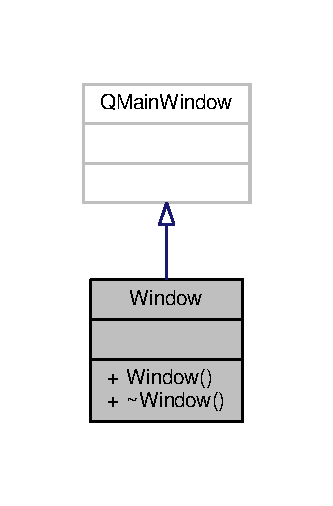
\includegraphics[width=160pt]{classWindow__inherit__graph}
\end{center}
\end{figure}


Collaboration diagram for Window\+:\nopagebreak
\begin{figure}[H]
\begin{center}
\leavevmode
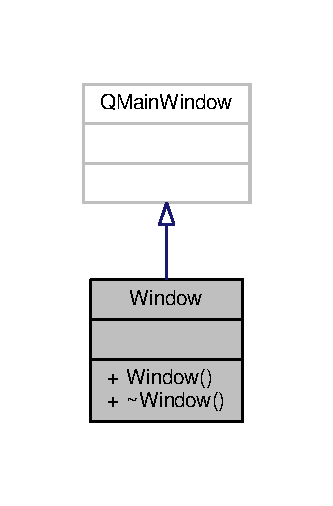
\includegraphics[width=160pt]{classWindow__coll__graph}
\end{center}
\end{figure}
\subsection*{Public Member Functions}
\begin{DoxyCompactItemize}
\item 
\hyperlink{classWindow_a8c86e48ef3180201cc97cb928abd66ca}{Window} (Q\+Widget $\ast$parent=nullptr)
\begin{DoxyCompactList}\small\item\em \hyperlink{classWindow}{Window} constructor. \end{DoxyCompactList}\item 
\hyperlink{classWindow_a245d821e6016fa1f6970ccbbedd635f6}{$\sim$\+Window} ()
\begin{DoxyCompactList}\small\item\em \hyperlink{classWindow}{Window} destructor. \end{DoxyCompactList}\end{DoxyCompactItemize}


\subsection{Detailed Description}
The \hyperlink{classWindow}{Window} class displays the login window and provides functionality for it. 

\subsection{Constructor \& Destructor Documentation}
\index{Window@{Window}!Window@{Window}}
\index{Window@{Window}!Window@{Window}}
\subsubsection[{\texorpdfstring{Window(\+Q\+Widget $\ast$parent=nullptr)}{Window(QWidget *parent=nullptr)}}]{\setlength{\rightskip}{0pt plus 5cm}Window\+::\+Window (
\begin{DoxyParamCaption}
\item[{Q\+Widget $\ast$}]{parent = {\ttfamily nullptr}}
\end{DoxyParamCaption}
)\hspace{0.3cm}{\ttfamily [explicit]}}\hypertarget{classWindow_a8c86e48ef3180201cc97cb928abd66ca}{}\label{classWindow_a8c86e48ef3180201cc97cb928abd66ca}


\hyperlink{classWindow}{Window} constructor. 


\begin{DoxyParams}{Parameters}
{\em parent} & window \\
\hline
\end{DoxyParams}
\index{Window@{Window}!````~Window@{$\sim$\+Window}}
\index{````~Window@{$\sim$\+Window}!Window@{Window}}
\subsubsection[{\texorpdfstring{$\sim$\+Window()}{~Window()}}]{\setlength{\rightskip}{0pt plus 5cm}Window\+::$\sim$\+Window (
\begin{DoxyParamCaption}
{}
\end{DoxyParamCaption}
)}\hypertarget{classWindow_a245d821e6016fa1f6970ccbbedd635f6}{}\label{classWindow_a245d821e6016fa1f6970ccbbedd635f6}


\hyperlink{classWindow}{Window} destructor. 



The documentation for this class was generated from the following files\+:\begin{DoxyCompactItemize}
\item 
Group Project/\+Scrum\+Of\+The\+Earth/\hyperlink{window_8h}{window.\+h}\item 
Group Project/\+Scrum\+Of\+The\+Earth/\hyperlink{admin__check_8cpp}{admin\+\_\+check.\+cpp}\item 
Group Project/\+Scrum\+Of\+The\+Earth/\hyperlink{create__login__file_8cpp}{create\+\_\+login\+\_\+file.\+cpp}\item 
Group Project/\+Scrum\+Of\+The\+Earth/\hyperlink{window_8cpp}{window.\+cpp}\end{DoxyCompactItemize}

\chapter{File Documentation}
\hypertarget{addshape_8cpp}{}\section{Group Project/\+Scrum\+Of\+The\+Earth/addshape.cpp File Reference}
\label{addshape_8cpp}\index{Group Project/\+Scrum\+Of\+The\+Earth/addshape.\+cpp@{Group Project/\+Scrum\+Of\+The\+Earth/addshape.\+cpp}}
{\ttfamily \#include \char`\"{}addshape.\+h\char`\"{}}\\*
{\ttfamily \#include \char`\"{}ui\+\_\+addshape.\+h\char`\"{}}\\*
{\ttfamily \#include \char`\"{}shape\+\_\+parser.\+h\char`\"{}}\\*
{\ttfamily \#include \char`\"{}getstrings.\+h\char`\"{}}\\*
Include dependency graph for addshape.\+cpp\+:\nopagebreak
\begin{figure}[H]
\begin{center}
\leavevmode
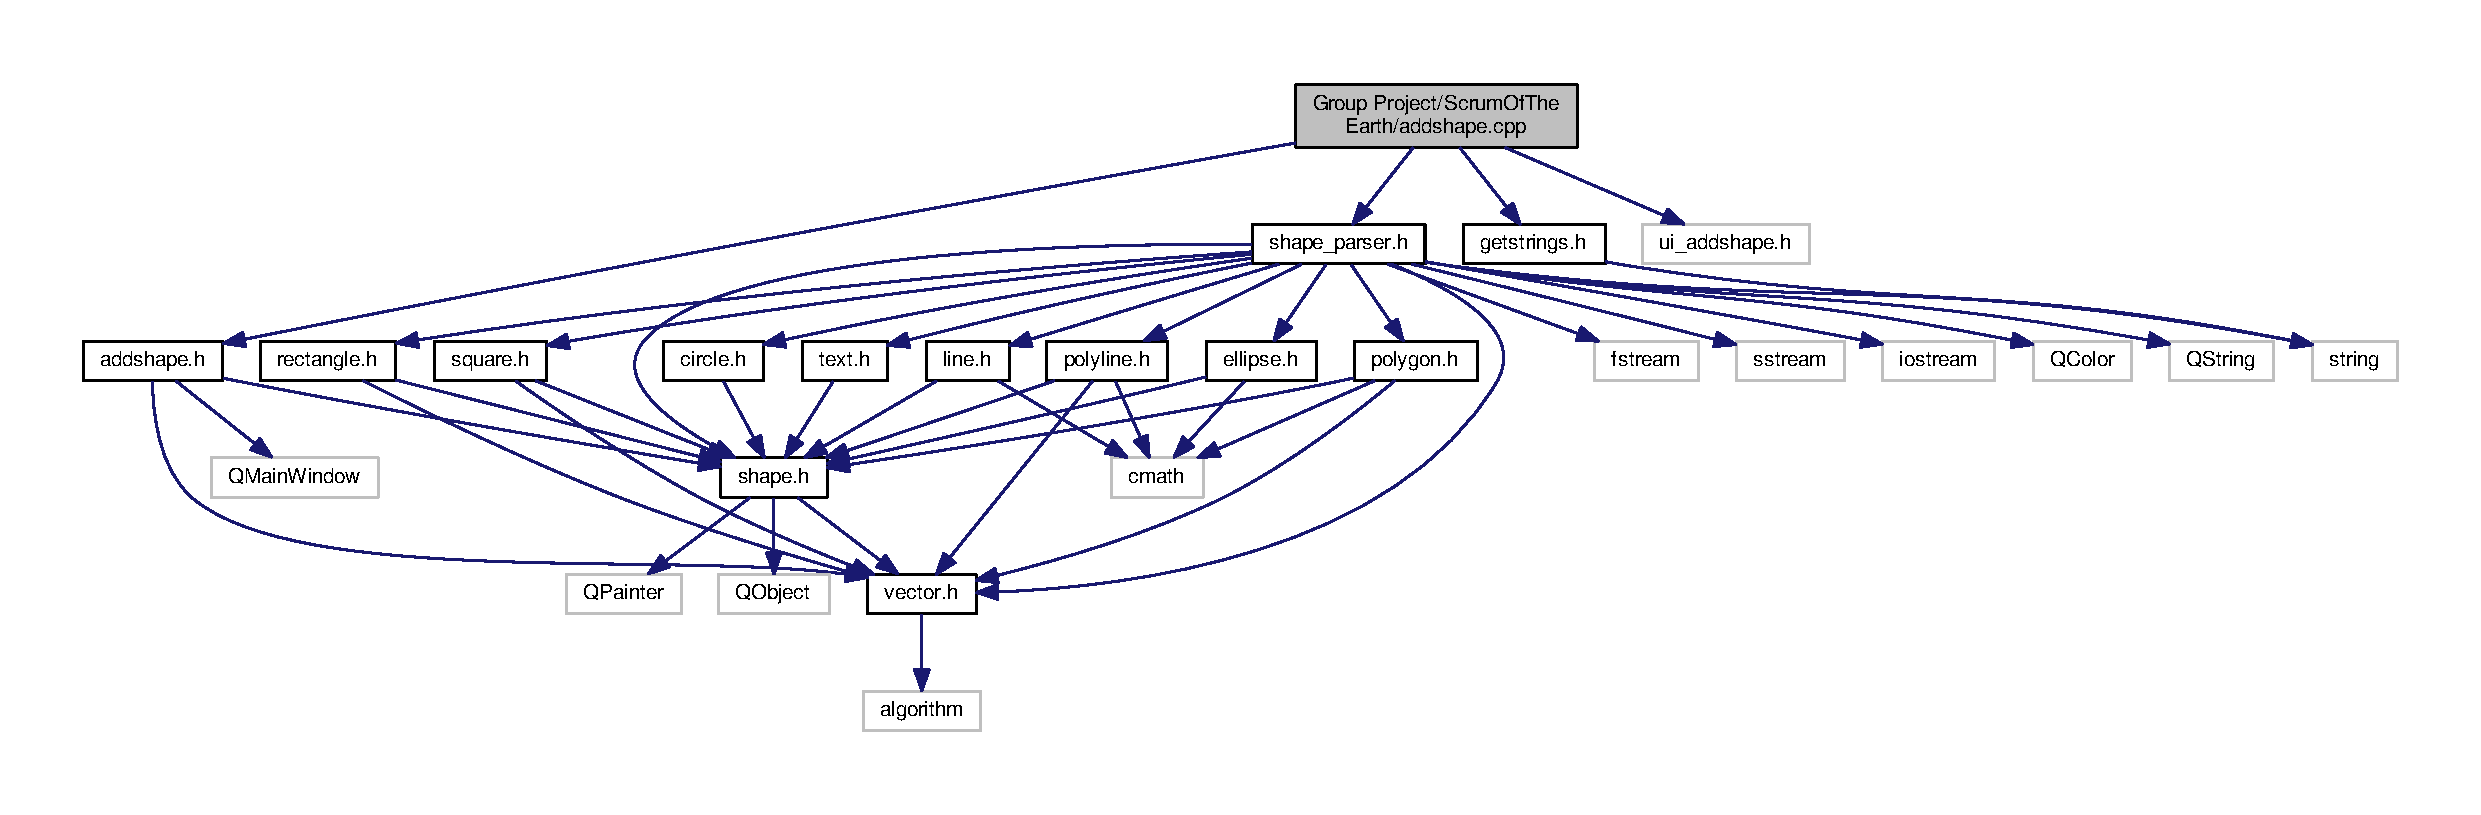
\includegraphics[width=350pt]{addshape_8cpp__incl}
\end{center}
\end{figure}

\hypertarget{addshape_8h}{}\section{Group Project/\+Scrum\+Of\+The\+Earth/addshape.h File Reference}
\label{addshape_8h}\index{Group Project/\+Scrum\+Of\+The\+Earth/addshape.\+h@{Group Project/\+Scrum\+Of\+The\+Earth/addshape.\+h}}
{\ttfamily \#include \char`\"{}vector.\+h\char`\"{}}\\*
{\ttfamily \#include \char`\"{}shape.\+h\char`\"{}}\\*
{\ttfamily \#include $<$Q\+Main\+Window$>$}\\*
Include dependency graph for addshape.\+h\+:\nopagebreak
\begin{figure}[H]
\begin{center}
\leavevmode
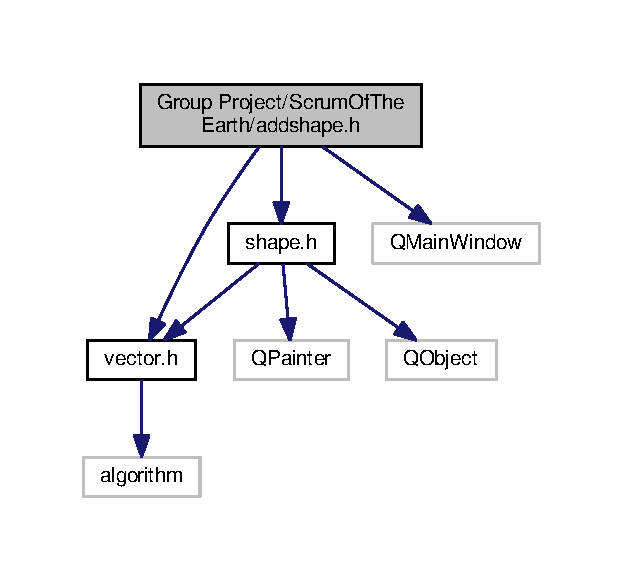
\includegraphics[width=299pt]{addshape_8h__incl}
\end{center}
\end{figure}
This graph shows which files directly or indirectly include this file\+:\nopagebreak
\begin{figure}[H]
\begin{center}
\leavevmode
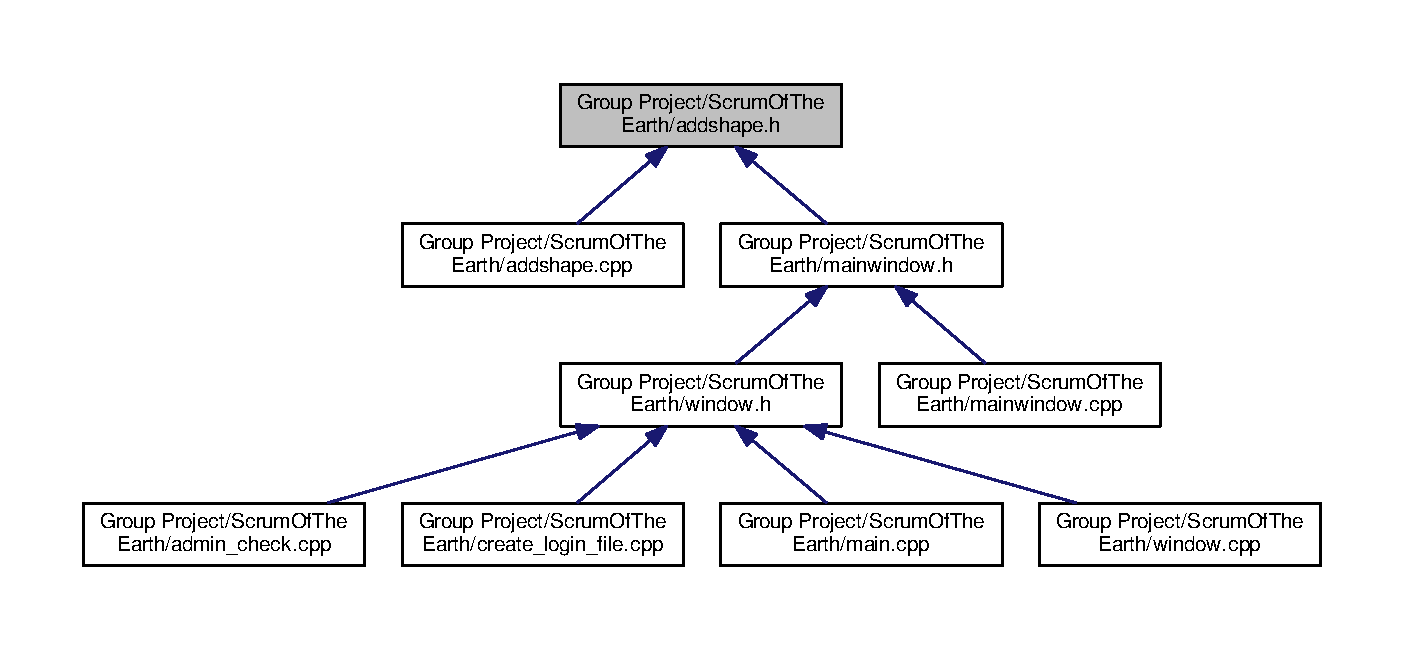
\includegraphics[width=350pt]{addshape_8h__dep__incl}
\end{center}
\end{figure}
\subsection*{Classes}
\begin{DoxyCompactItemize}
\item 
class \hyperlink{classAddShape}{Add\+Shape}
\begin{DoxyCompactList}\small\item\em \hyperlink{classAddShape}{Add\+Shape} class that provides functionality for the add shape button. \end{DoxyCompactList}\end{DoxyCompactItemize}
\subsection*{Namespaces}
\begin{DoxyCompactItemize}
\item 
 \hyperlink{namespaceUi}{Ui}
\end{DoxyCompactItemize}

\hypertarget{admin__check_8cpp}{}\section{Group Project/\+Scrum\+Of\+The\+Earth/admin\+\_\+check.cpp File Reference}
\label{admin__check_8cpp}\index{Group Project/\+Scrum\+Of\+The\+Earth/admin\+\_\+check.\+cpp@{Group Project/\+Scrum\+Of\+The\+Earth/admin\+\_\+check.\+cpp}}
{\ttfamily \#include \char`\"{}window.\+h\char`\"{}}\\*
{\ttfamily \#include $<$fstream$>$}\\*
Include dependency graph for admin\+\_\+check.\+cpp\+:\nopagebreak
\begin{figure}[H]
\begin{center}
\leavevmode
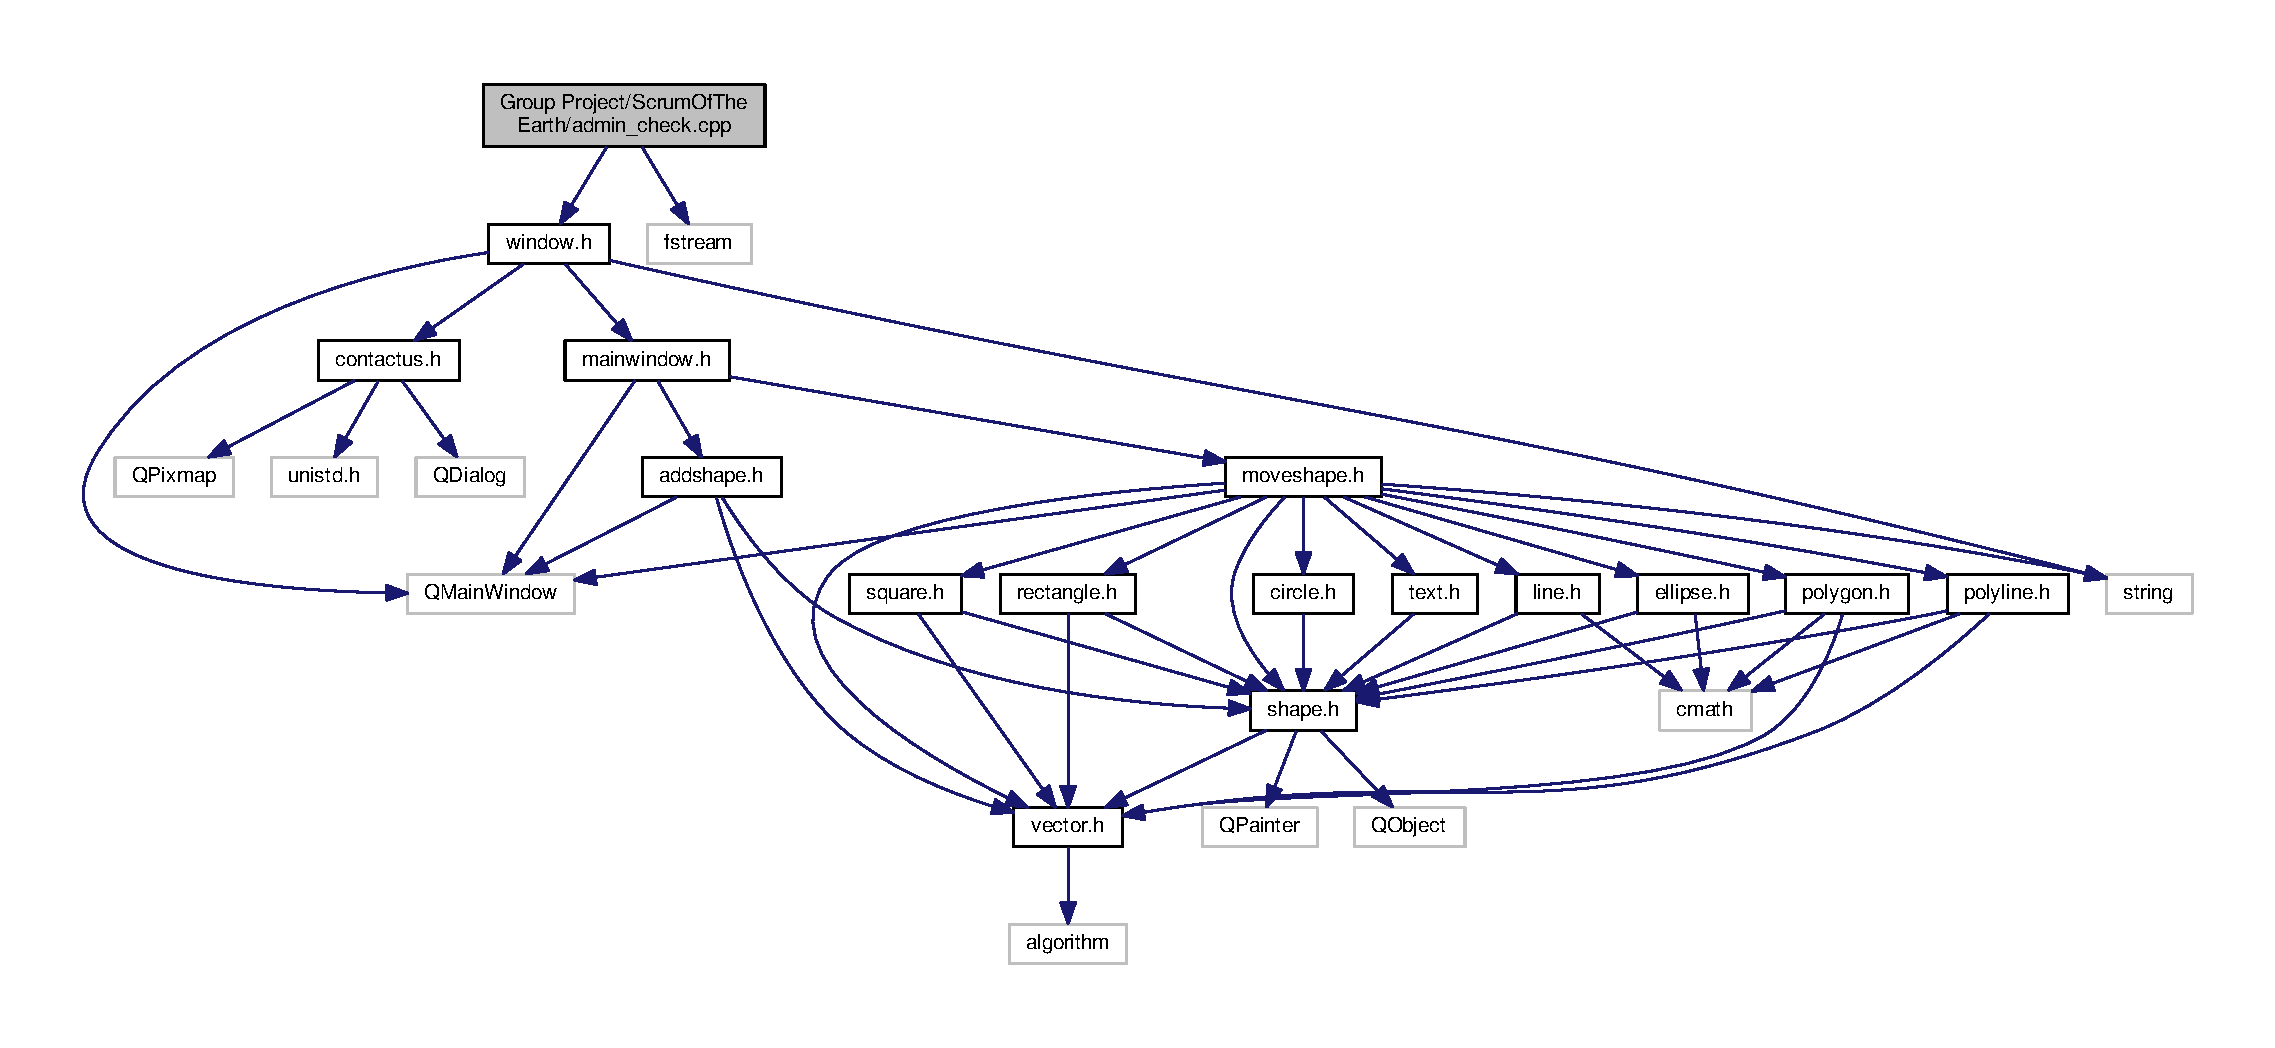
\includegraphics[width=350pt]{admin__check_8cpp__incl}
\end{center}
\end{figure}

\hypertarget{admin__list_8txt}{}\section{Group Project/\+Scrum\+Of\+The\+Earth/admin\+\_\+list.txt File Reference}
\label{admin__list_8txt}\index{Group Project/\+Scrum\+Of\+The\+Earth/admin\+\_\+list.\+txt@{Group Project/\+Scrum\+Of\+The\+Earth/admin\+\_\+list.\+txt}}

\hypertarget{circle_8cpp}{}\section{Group Project/\+Scrum\+Of\+The\+Earth/circle.cpp File Reference}
\label{circle_8cpp}\index{Group Project/\+Scrum\+Of\+The\+Earth/circle.\+cpp@{Group Project/\+Scrum\+Of\+The\+Earth/circle.\+cpp}}
{\ttfamily \#include \char`\"{}circle.\+h\char`\"{}}\\*
{\ttfamily \#include $<$string$>$}\\*
Include dependency graph for circle.\+cpp\+:\nopagebreak
\begin{figure}[H]
\begin{center}
\leavevmode
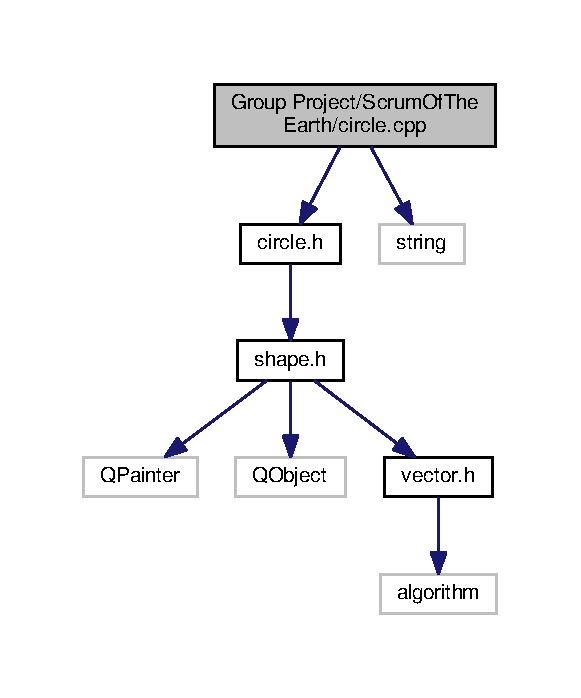
\includegraphics[width=279pt]{circle_8cpp__incl}
\end{center}
\end{figure}

\hypertarget{circle_8h}{}\section{Group Project/\+Scrum\+Of\+The\+Earth/circle.h File Reference}
\label{circle_8h}\index{Group Project/\+Scrum\+Of\+The\+Earth/circle.\+h@{Group Project/\+Scrum\+Of\+The\+Earth/circle.\+h}}
{\ttfamily \#include \char`\"{}shape.\+h\char`\"{}}\\*
Include dependency graph for circle.\+h\+:\nopagebreak
\begin{figure}[H]
\begin{center}
\leavevmode
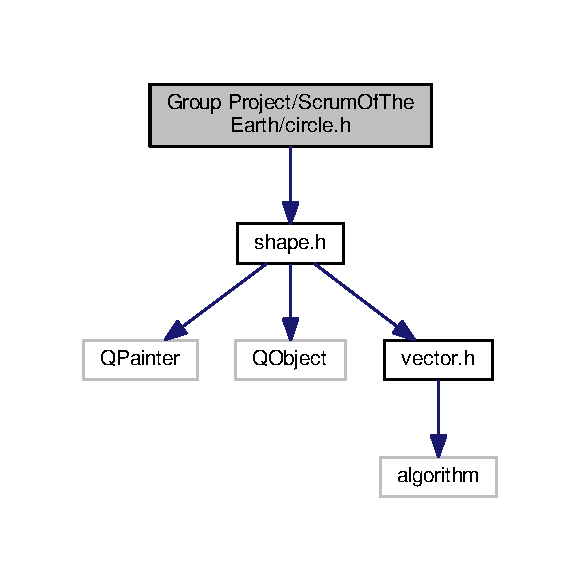
\includegraphics[width=279pt]{circle_8h__incl}
\end{center}
\end{figure}
This graph shows which files directly or indirectly include this file\+:\nopagebreak
\begin{figure}[H]
\begin{center}
\leavevmode
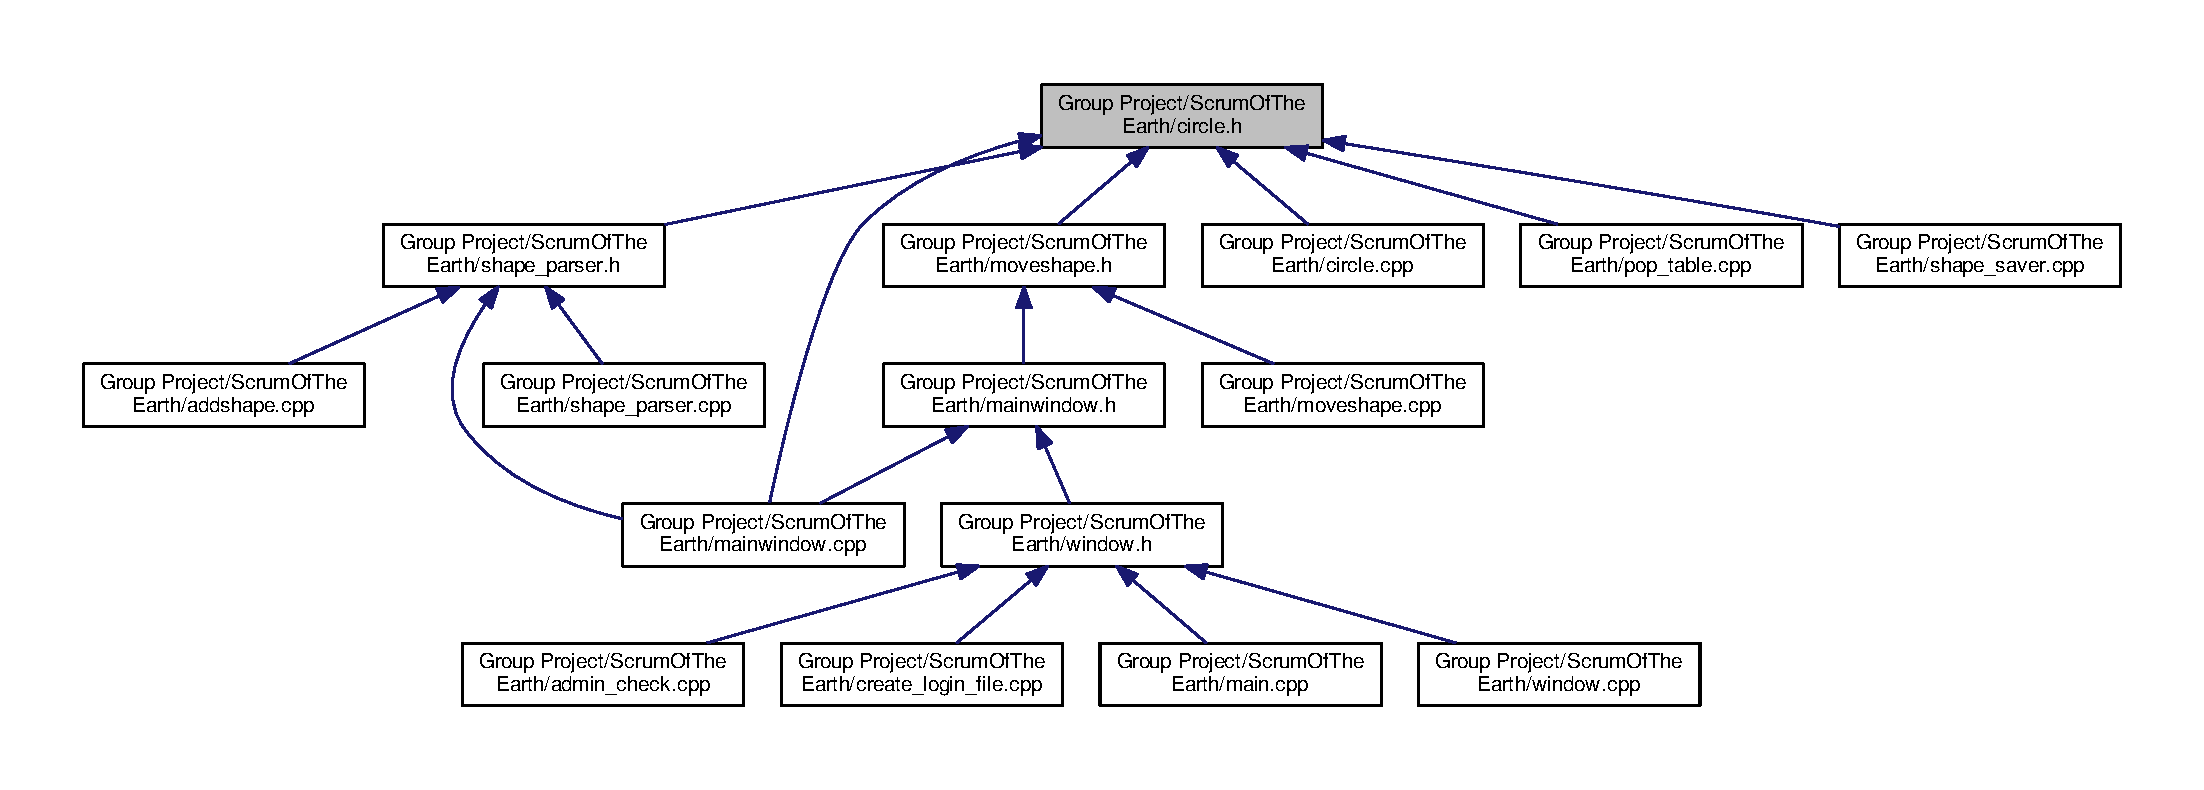
\includegraphics[width=350pt]{circle_8h__dep__incl}
\end{center}
\end{figure}
\subsection*{Classes}
\begin{DoxyCompactItemize}
\item 
class \hyperlink{classCircle}{Circle}
\begin{DoxyCompactList}\small\item\em \hyperlink{classCircle}{Circle} class that Q\+Painter can draw. \end{DoxyCompactList}\end{DoxyCompactItemize}

\hypertarget{contactus_8cpp}{}\section{Group Project/\+Scrum\+Of\+The\+Earth/contactus.cpp File Reference}
\label{contactus_8cpp}\index{Group Project/\+Scrum\+Of\+The\+Earth/contactus.\+cpp@{Group Project/\+Scrum\+Of\+The\+Earth/contactus.\+cpp}}
{\ttfamily \#include \char`\"{}contactus.\+h\char`\"{}}\\*
{\ttfamily \#include \char`\"{}ui\+\_\+contactus.\+h\char`\"{}}\\*
{\ttfamily \#include $<$limits.\+h$>$}\\*
{\ttfamily \#include $<$stdlib.\+h$>$}\\*
{\ttfamily \#include $<$string.\+h$>$}\\*
Include dependency graph for contactus.\+cpp\+:\nopagebreak
\begin{figure}[H]
\begin{center}
\leavevmode
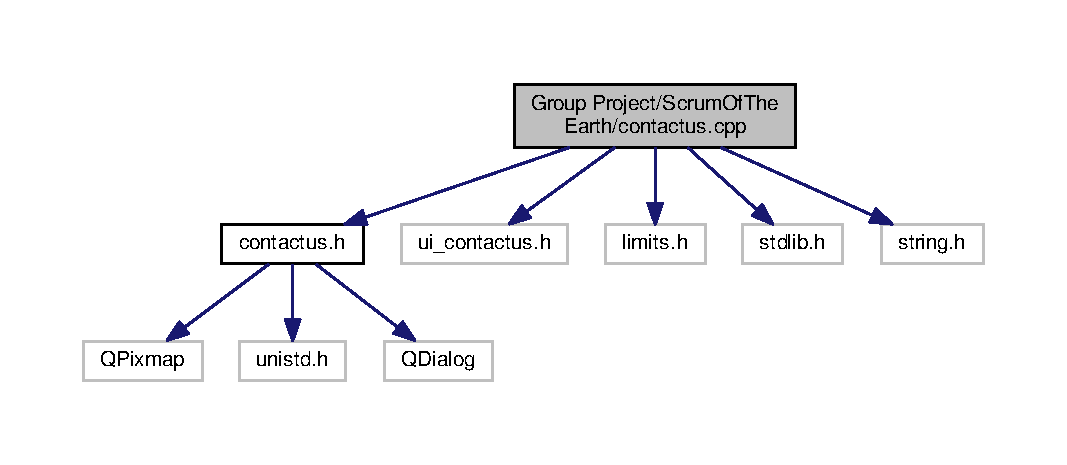
\includegraphics[width=350pt]{contactus_8cpp__incl}
\end{center}
\end{figure}

\hypertarget{contactus_8h}{}\section{Group Project/\+Scrum\+Of\+The\+Earth/contactus.h File Reference}
\label{contactus_8h}\index{Group Project/\+Scrum\+Of\+The\+Earth/contactus.\+h@{Group Project/\+Scrum\+Of\+The\+Earth/contactus.\+h}}
{\ttfamily \#include $<$Q\+Pixmap$>$}\\*
{\ttfamily \#include $<$unistd.\+h$>$}\\*
{\ttfamily \#include $<$Q\+Dialog$>$}\\*
Include dependency graph for contactus.\+h\+:\nopagebreak
\begin{figure}[H]
\begin{center}
\leavevmode
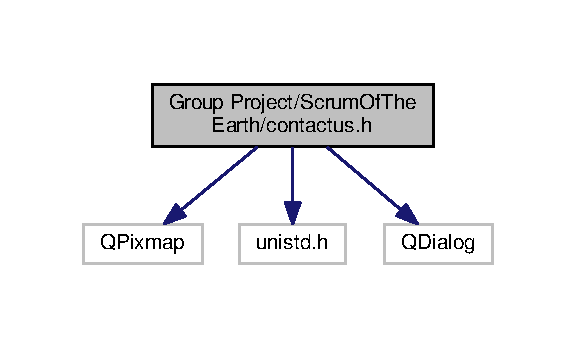
\includegraphics[width=277pt]{contactus_8h__incl}
\end{center}
\end{figure}
This graph shows which files directly or indirectly include this file\+:\nopagebreak
\begin{figure}[H]
\begin{center}
\leavevmode
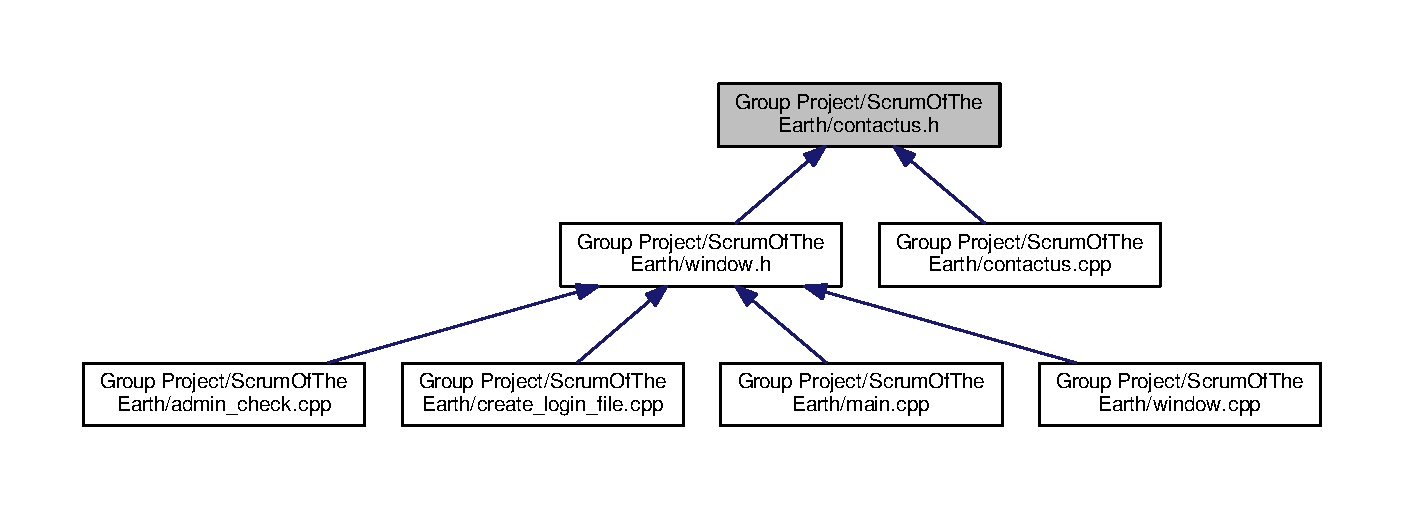
\includegraphics[width=350pt]{contactus_8h__dep__incl}
\end{center}
\end{figure}
\subsection*{Classes}
\begin{DoxyCompactItemize}
\item 
class \hyperlink{classContactUs}{Contact\+Us}
\begin{DoxyCompactList}\small\item\em The \hyperlink{classContactUs}{Contact\+Us} class provides functionality for the contact us window. \end{DoxyCompactList}\end{DoxyCompactItemize}
\subsection*{Namespaces}
\begin{DoxyCompactItemize}
\item 
 \hyperlink{namespaceUi}{Ui}
\end{DoxyCompactItemize}

\hypertarget{create__login__file_8cpp}{}\section{Group Project/\+Scrum\+Of\+The\+Earth/create\+\_\+login\+\_\+file.cpp File Reference}
\label{create__login__file_8cpp}\index{Group Project/\+Scrum\+Of\+The\+Earth/create\+\_\+login\+\_\+file.\+cpp@{Group Project/\+Scrum\+Of\+The\+Earth/create\+\_\+login\+\_\+file.\+cpp}}
{\ttfamily \#include \char`\"{}window.\+h\char`\"{}}\\*
{\ttfamily \#include $<$fstream$>$}\\*
Include dependency graph for create\+\_\+login\+\_\+file.\+cpp\+:\nopagebreak
\begin{figure}[H]
\begin{center}
\leavevmode
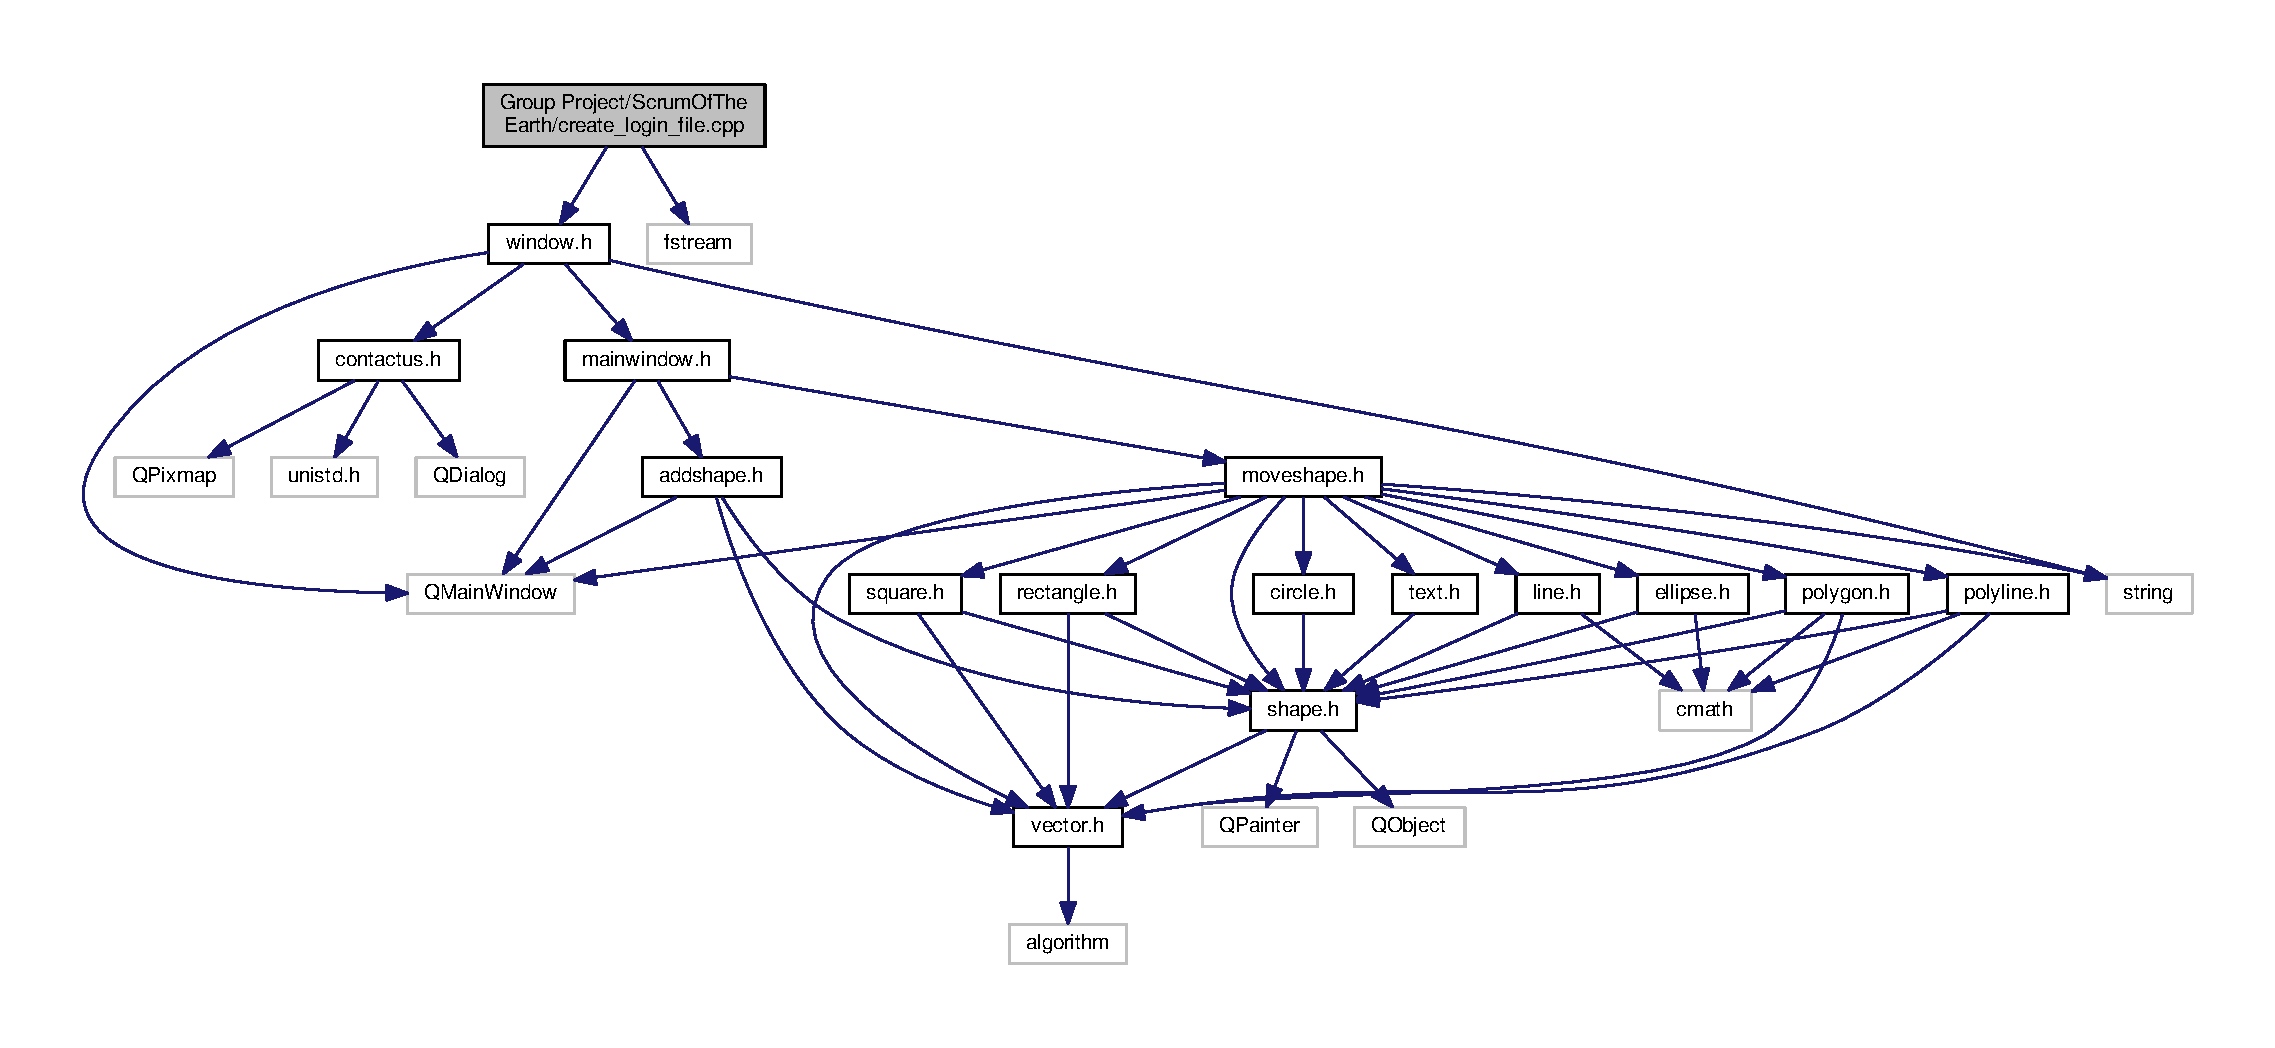
\includegraphics[width=350pt]{create__login__file_8cpp__incl}
\end{center}
\end{figure}

\hypertarget{delete__zeros_8cpp}{}\section{Group Project/\+Scrum\+Of\+The\+Earth/delete\+\_\+zeros.cpp File Reference}
\label{delete__zeros_8cpp}\index{Group Project/\+Scrum\+Of\+The\+Earth/delete\+\_\+zeros.\+cpp@{Group Project/\+Scrum\+Of\+The\+Earth/delete\+\_\+zeros.\+cpp}}
{\ttfamily \#include \char`\"{}delete\+\_\+zeros.\+h\char`\"{}}\\*
Include dependency graph for delete\+\_\+zeros.\+cpp\+:\nopagebreak
\begin{figure}[H]
\begin{center}
\leavevmode
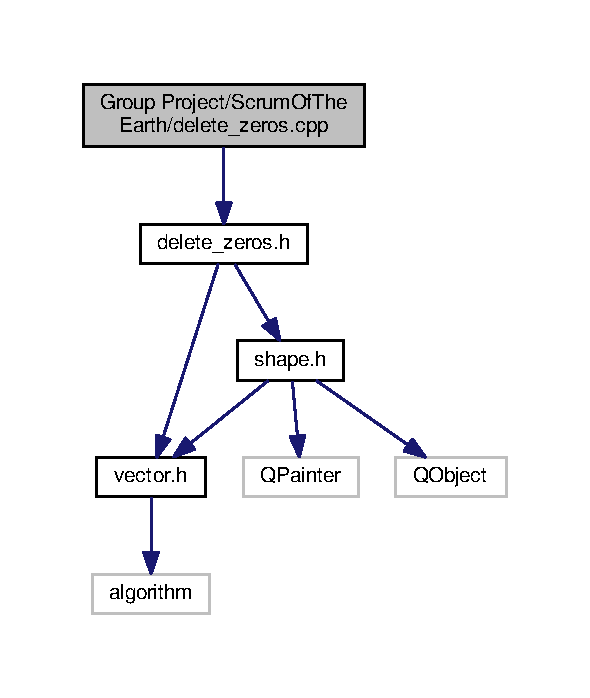
\includegraphics[width=283pt]{delete__zeros_8cpp__incl}
\end{center}
\end{figure}
\subsection*{Functions}
\begin{DoxyCompactItemize}
\item 
void \hyperlink{delete__zeros_8cpp_a9dec4a09977f70bba53ccc9eb789f752}{delete\+\_\+\+Azeros} (\hyperlink{classmyStd_1_1vector}{my\+Std\+::vector}$<$ \hyperlink{classShape}{Shape} $\ast$ $>$ \&vec)
\begin{DoxyCompactList}\small\item\em delete\+\_\+\+Azeros erases any shape with zero area in a vector of \hyperlink{classShape}{Shape} Pointers \end{DoxyCompactList}\item 
void \hyperlink{delete__zeros_8cpp_afcfd6fbd3a7dab9bdb3ddf2ac08d7586}{delete\+\_\+\+Pzeros} (\hyperlink{classmyStd_1_1vector}{my\+Std\+::vector}$<$ \hyperlink{classShape}{Shape} $\ast$ $>$ \&vec)
\begin{DoxyCompactList}\small\item\em delete\+\_\+\+Pzeros erases any shape with zero perimeter in a vector of \hyperlink{classShape}{Shape} Pointers \end{DoxyCompactList}\end{DoxyCompactItemize}


\subsection{Function Documentation}
\index{delete\+\_\+zeros.\+cpp@{delete\+\_\+zeros.\+cpp}!delete\+\_\+\+Azeros@{delete\+\_\+\+Azeros}}
\index{delete\+\_\+\+Azeros@{delete\+\_\+\+Azeros}!delete\+\_\+zeros.\+cpp@{delete\+\_\+zeros.\+cpp}}
\subsubsection[{\texorpdfstring{delete\+\_\+\+Azeros(my\+Std\+::vector$<$ Shape $\ast$ $>$ \&vec)}{delete_Azeros(myStd::vector< Shape * > &vec)}}]{\setlength{\rightskip}{0pt plus 5cm}void delete\+\_\+\+Azeros (
\begin{DoxyParamCaption}
\item[{{\bf my\+Std\+::vector}$<$ {\bf Shape} $\ast$ $>$ \&}]{vec}
\end{DoxyParamCaption}
)}\hypertarget{delete__zeros_8cpp_a9dec4a09977f70bba53ccc9eb789f752}{}\label{delete__zeros_8cpp_a9dec4a09977f70bba53ccc9eb789f752}


delete\+\_\+\+Azeros erases any shape with zero area in a vector of \hyperlink{classShape}{Shape} Pointers 

\index{delete\+\_\+zeros.\+cpp@{delete\+\_\+zeros.\+cpp}!delete\+\_\+\+Pzeros@{delete\+\_\+\+Pzeros}}
\index{delete\+\_\+\+Pzeros@{delete\+\_\+\+Pzeros}!delete\+\_\+zeros.\+cpp@{delete\+\_\+zeros.\+cpp}}
\subsubsection[{\texorpdfstring{delete\+\_\+\+Pzeros(my\+Std\+::vector$<$ Shape $\ast$ $>$ \&vec)}{delete_Pzeros(myStd::vector< Shape * > &vec)}}]{\setlength{\rightskip}{0pt plus 5cm}void delete\+\_\+\+Pzeros (
\begin{DoxyParamCaption}
\item[{{\bf my\+Std\+::vector}$<$ {\bf Shape} $\ast$ $>$ \&}]{vec}
\end{DoxyParamCaption}
)}\hypertarget{delete__zeros_8cpp_afcfd6fbd3a7dab9bdb3ddf2ac08d7586}{}\label{delete__zeros_8cpp_afcfd6fbd3a7dab9bdb3ddf2ac08d7586}


delete\+\_\+\+Pzeros erases any shape with zero perimeter in a vector of \hyperlink{classShape}{Shape} Pointers 


\hypertarget{delete__zeros_8h}{}\section{Group Project/\+Scrum\+Of\+The\+Earth/delete\+\_\+zeros.h File Reference}
\label{delete__zeros_8h}\index{Group Project/\+Scrum\+Of\+The\+Earth/delete\+\_\+zeros.\+h@{Group Project/\+Scrum\+Of\+The\+Earth/delete\+\_\+zeros.\+h}}
{\ttfamily \#include \char`\"{}vector.\+h\char`\"{}}\\*
{\ttfamily \#include \char`\"{}shape.\+h\char`\"{}}\\*
Include dependency graph for delete\+\_\+zeros.\+h\+:\nopagebreak
\begin{figure}[H]
\begin{center}
\leavevmode
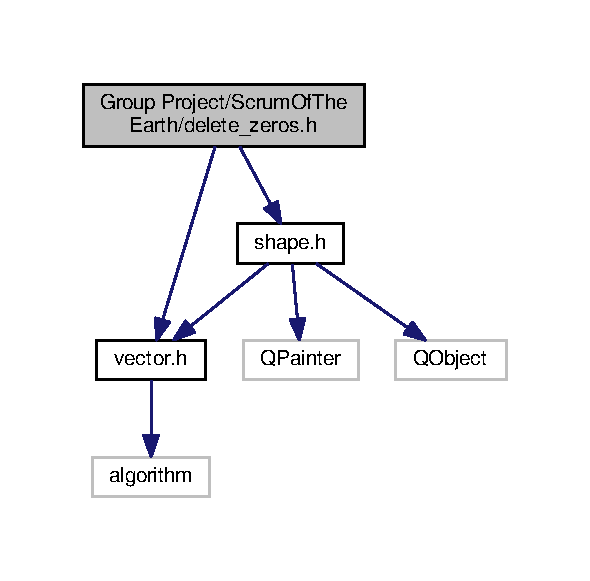
\includegraphics[width=283pt]{delete__zeros_8h__incl}
\end{center}
\end{figure}
This graph shows which files directly or indirectly include this file\+:\nopagebreak
\begin{figure}[H]
\begin{center}
\leavevmode
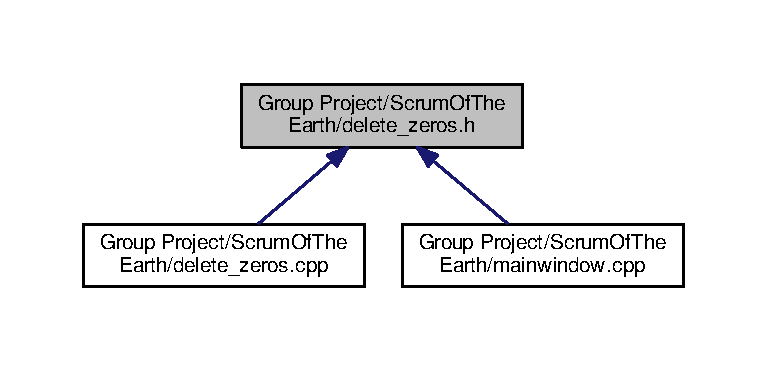
\includegraphics[width=350pt]{delete__zeros_8h__dep__incl}
\end{center}
\end{figure}
\subsection*{Functions}
\begin{DoxyCompactItemize}
\item 
void \hyperlink{delete__zeros_8h_a4ebed1107b5a6f70d9dc7afaaba35565}{delete\+\_\+\+Azeros} (\hyperlink{classmyStd_1_1vector}{my\+Std\+::vector}$<$ \hyperlink{classShape}{Shape} $\ast$ $>$ \&)
\begin{DoxyCompactList}\small\item\em delete\+\_\+\+Azeros erases any shape with zero area in a vector of \hyperlink{classShape}{Shape} Pointers \end{DoxyCompactList}\item 
void \hyperlink{delete__zeros_8h_a2a244a091a5ebad5b1cefbe45d4296df}{delete\+\_\+\+Pzeros} (\hyperlink{classmyStd_1_1vector}{my\+Std\+::vector}$<$ \hyperlink{classShape}{Shape} $\ast$ $>$ \&)
\begin{DoxyCompactList}\small\item\em delete\+\_\+\+Pzeros erases any shape with zero perimeter in a vector of \hyperlink{classShape}{Shape} Pointers \end{DoxyCompactList}\end{DoxyCompactItemize}


\subsection{Function Documentation}
\index{delete\+\_\+zeros.\+h@{delete\+\_\+zeros.\+h}!delete\+\_\+\+Azeros@{delete\+\_\+\+Azeros}}
\index{delete\+\_\+\+Azeros@{delete\+\_\+\+Azeros}!delete\+\_\+zeros.\+h@{delete\+\_\+zeros.\+h}}
\subsubsection[{\texorpdfstring{delete\+\_\+\+Azeros(my\+Std\+::vector$<$ Shape $\ast$ $>$ \&)}{delete_Azeros(myStd::vector< Shape * > &)}}]{\setlength{\rightskip}{0pt plus 5cm}void delete\+\_\+\+Azeros (
\begin{DoxyParamCaption}
\item[{{\bf my\+Std\+::vector}$<$ {\bf Shape} $\ast$ $>$ \&}]{}
\end{DoxyParamCaption}
)}\hypertarget{delete__zeros_8h_a4ebed1107b5a6f70d9dc7afaaba35565}{}\label{delete__zeros_8h_a4ebed1107b5a6f70d9dc7afaaba35565}


delete\+\_\+\+Azeros erases any shape with zero area in a vector of \hyperlink{classShape}{Shape} Pointers 

\index{delete\+\_\+zeros.\+h@{delete\+\_\+zeros.\+h}!delete\+\_\+\+Pzeros@{delete\+\_\+\+Pzeros}}
\index{delete\+\_\+\+Pzeros@{delete\+\_\+\+Pzeros}!delete\+\_\+zeros.\+h@{delete\+\_\+zeros.\+h}}
\subsubsection[{\texorpdfstring{delete\+\_\+\+Pzeros(my\+Std\+::vector$<$ Shape $\ast$ $>$ \&)}{delete_Pzeros(myStd::vector< Shape * > &)}}]{\setlength{\rightskip}{0pt plus 5cm}void delete\+\_\+\+Pzeros (
\begin{DoxyParamCaption}
\item[{{\bf my\+Std\+::vector}$<$ {\bf Shape} $\ast$ $>$ \&}]{}
\end{DoxyParamCaption}
)}\hypertarget{delete__zeros_8h_a2a244a091a5ebad5b1cefbe45d4296df}{}\label{delete__zeros_8h_a2a244a091a5ebad5b1cefbe45d4296df}


delete\+\_\+\+Pzeros erases any shape with zero perimeter in a vector of \hyperlink{classShape}{Shape} Pointers 


\hypertarget{doxygen__log_8txt}{}\section{Group Project/\+Scrum\+Of\+The\+Earth/doxygen\+\_\+log.txt File Reference}
\label{doxygen__log_8txt}\index{Group Project/\+Scrum\+Of\+The\+Earth/doxygen\+\_\+log.\+txt@{Group Project/\+Scrum\+Of\+The\+Earth/doxygen\+\_\+log.\+txt}}

\hypertarget{ellipse_8cpp}{}\section{Group Project/\+Scrum\+Of\+The\+Earth/ellipse.cpp File Reference}
\label{ellipse_8cpp}\index{Group Project/\+Scrum\+Of\+The\+Earth/ellipse.\+cpp@{Group Project/\+Scrum\+Of\+The\+Earth/ellipse.\+cpp}}
{\ttfamily \#include \char`\"{}ellipse.\+h\char`\"{}}\\*
Include dependency graph for ellipse.\+cpp\+:\nopagebreak
\begin{figure}[H]
\begin{center}
\leavevmode
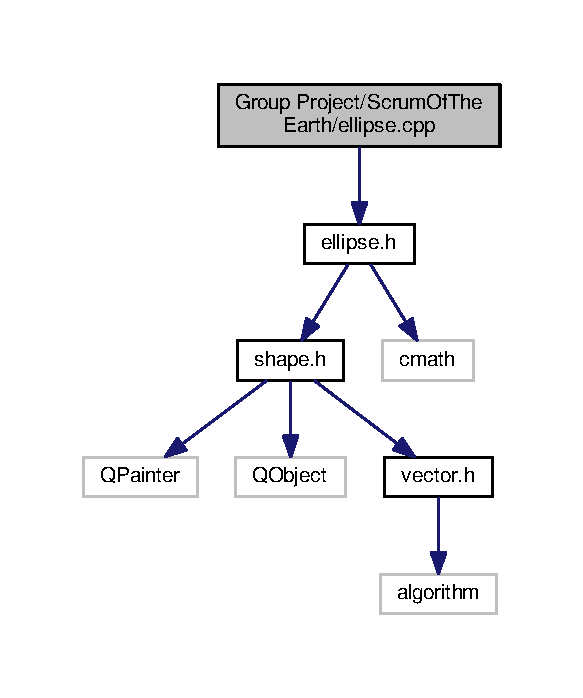
\includegraphics[width=280pt]{ellipse_8cpp__incl}
\end{center}
\end{figure}

\hypertarget{ellipse_8h}{}\section{Group Project/\+Scrum\+Of\+The\+Earth/ellipse.h File Reference}
\label{ellipse_8h}\index{Group Project/\+Scrum\+Of\+The\+Earth/ellipse.\+h@{Group Project/\+Scrum\+Of\+The\+Earth/ellipse.\+h}}
{\ttfamily \#include \char`\"{}shape.\+h\char`\"{}}\\*
{\ttfamily \#include $<$cmath$>$}\\*
Include dependency graph for ellipse.\+h\+:\nopagebreak
\begin{figure}[H]
\begin{center}
\leavevmode
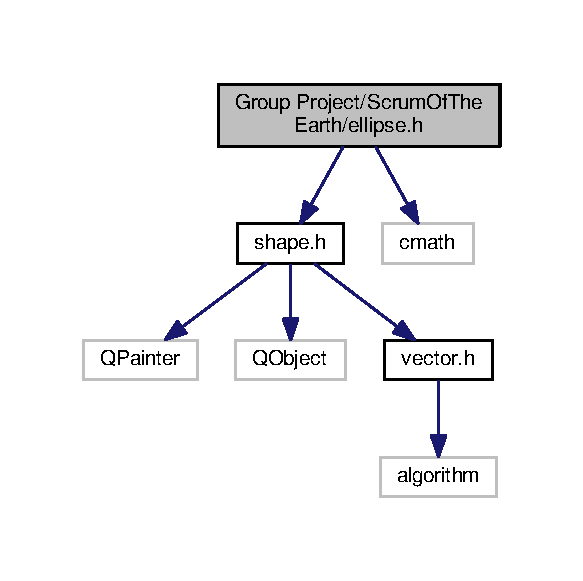
\includegraphics[width=280pt]{ellipse_8h__incl}
\end{center}
\end{figure}
This graph shows which files directly or indirectly include this file\+:\nopagebreak
\begin{figure}[H]
\begin{center}
\leavevmode
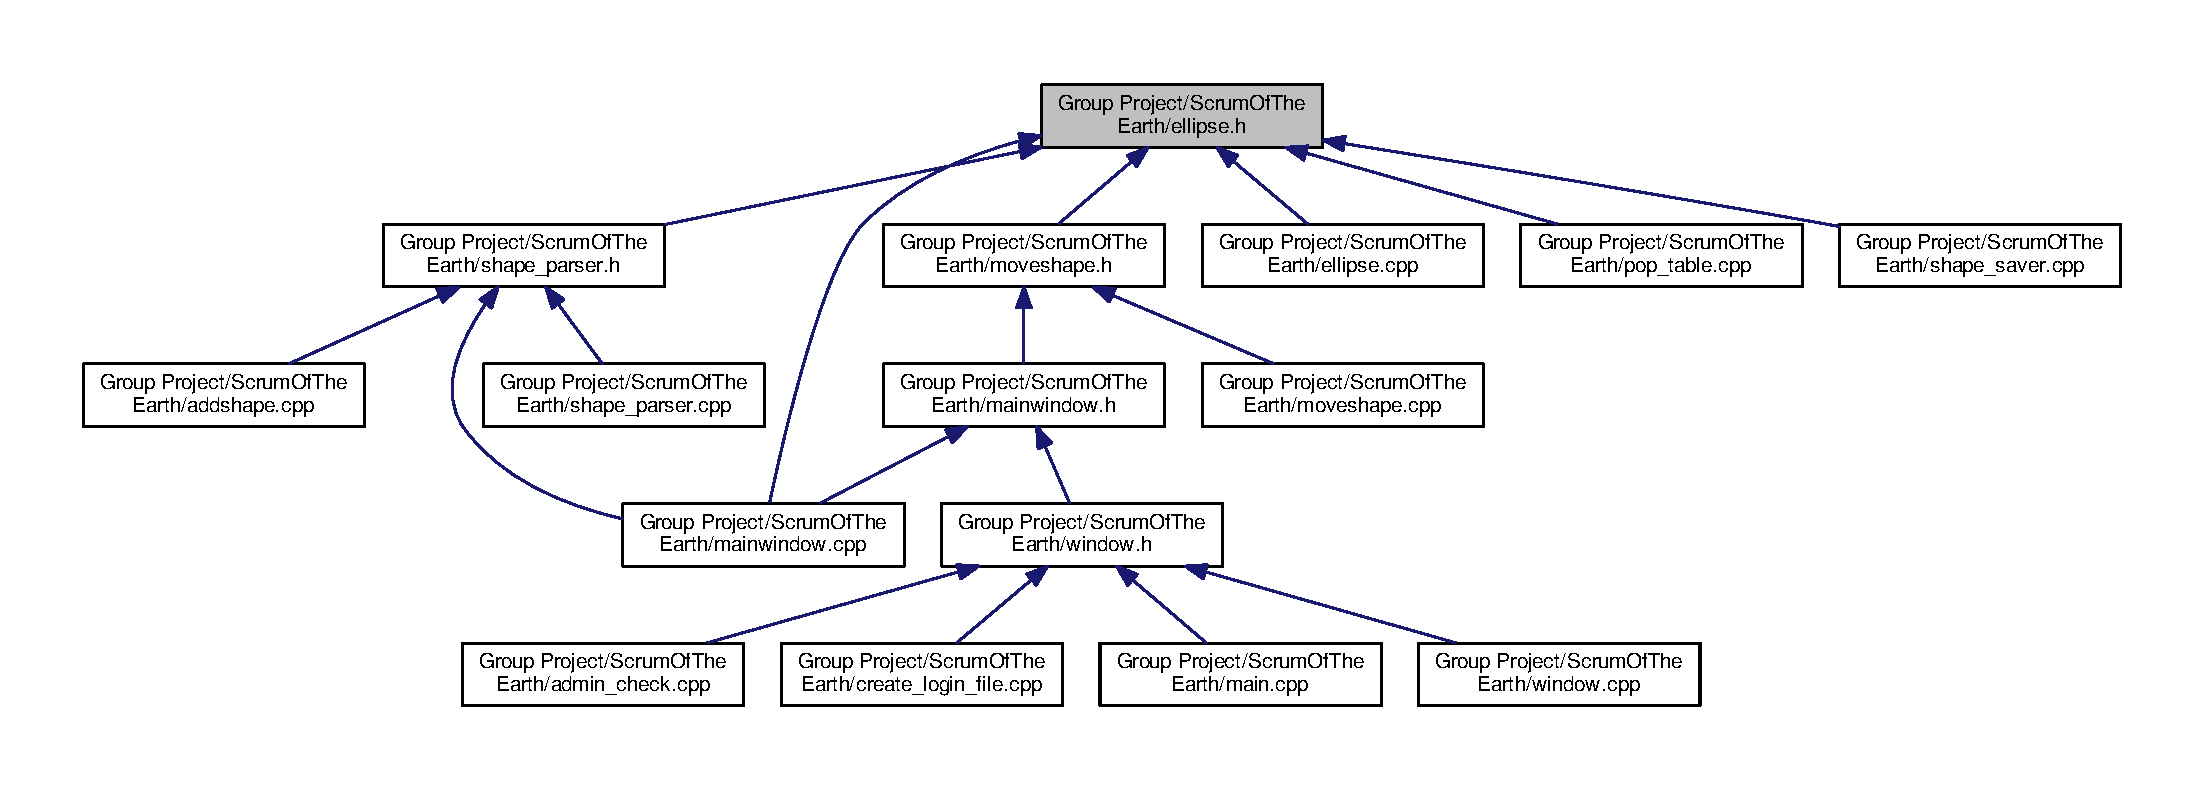
\includegraphics[width=350pt]{ellipse_8h__dep__incl}
\end{center}
\end{figure}
\subsection*{Classes}
\begin{DoxyCompactItemize}
\item 
class \hyperlink{classEllipse}{Ellipse}
\begin{DoxyCompactList}\small\item\em \hyperlink{classEllipse}{Ellipse} class that Q\+Painter can draw. \end{DoxyCompactList}\end{DoxyCompactItemize}

\hypertarget{getstrings_8cpp}{}\section{Group Project/\+Scrum\+Of\+The\+Earth/getstrings.cpp File Reference}
\label{getstrings_8cpp}\index{Group Project/\+Scrum\+Of\+The\+Earth/getstrings.\+cpp@{Group Project/\+Scrum\+Of\+The\+Earth/getstrings.\+cpp}}
{\ttfamily \#include \char`\"{}getstrings.\+h\char`\"{}}\\*
Include dependency graph for getstrings.\+cpp\+:\nopagebreak
\begin{figure}[H]
\begin{center}
\leavevmode
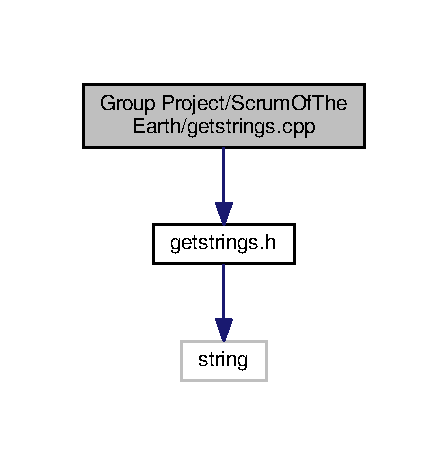
\includegraphics[width=215pt]{getstrings_8cpp__incl}
\end{center}
\end{figure}
\subsection*{Functions}
\begin{DoxyCompactItemize}
\item 
std\+::string \hyperlink{getstrings_8cpp_ae2e8c725725c53aced4754efb1ba3297}{get\+Pen\+Style} (int ps)
\begin{DoxyCompactList}\small\item\em Converts an index to a string for a penstyle. \end{DoxyCompactList}\item 
std\+::string \hyperlink{getstrings_8cpp_a36f20d2b33b32e3051b9439984fa3dc1}{get\+Color} (int color)
\begin{DoxyCompactList}\small\item\em Converts an index to a string for a color. \end{DoxyCompactList}\item 
std\+::string \hyperlink{getstrings_8cpp_ab55986fc16e82140cc960949e8d98fc3}{get\+Pen\+Cap\+Style} (int pcs)
\begin{DoxyCompactList}\small\item\em Converts an index to a string for a pen cap style. \end{DoxyCompactList}\item 
std\+::string \hyperlink{getstrings_8cpp_a59c542c498dce52daab6c95e393084f7}{get\+Pen\+Join\+Style} (int pjs)
\begin{DoxyCompactList}\small\item\em Converts an index to a string for a pen join style. \end{DoxyCompactList}\item 
std\+::string \hyperlink{getstrings_8cpp_a59572458de7eabcb211b12647cd8cc67}{get\+Brush\+Style} (int bs)
\begin{DoxyCompactList}\small\item\em Converts an index to a string for a brush style. \end{DoxyCompactList}\item 
std\+::string \hyperlink{getstrings_8cpp_ab73fa4f5c93f8a3c34cc0a3aaf7508d8}{get\+Text\+Alignment} (int ta)
\begin{DoxyCompactList}\small\item\em Converts an index to a string for a text alignment. \end{DoxyCompactList}\item 
std\+::string \hyperlink{getstrings_8cpp_a362dd7a8956d7364df5cce0070ec15ca}{get\+Font\+Style} (int fs)
\begin{DoxyCompactList}\small\item\em Converts an index to a string for a font style. \end{DoxyCompactList}\item 
std\+::string \hyperlink{getstrings_8cpp_a4d2ad0fcdf9ccdd1fdb8f8da293f051d}{get\+Font\+Weight} (int fw)
\begin{DoxyCompactList}\small\item\em Converts an index to a string for font weight. \end{DoxyCompactList}\end{DoxyCompactItemize}


\subsection{Function Documentation}
\index{getstrings.\+cpp@{getstrings.\+cpp}!get\+Brush\+Style@{get\+Brush\+Style}}
\index{get\+Brush\+Style@{get\+Brush\+Style}!getstrings.\+cpp@{getstrings.\+cpp}}
\subsubsection[{\texorpdfstring{get\+Brush\+Style(int bs)}{getBrushStyle(int bs)}}]{\setlength{\rightskip}{0pt plus 5cm}std\+::string get\+Brush\+Style (
\begin{DoxyParamCaption}
\item[{int}]{bs}
\end{DoxyParamCaption}
)}\hypertarget{getstrings_8cpp_a59572458de7eabcb211b12647cd8cc67}{}\label{getstrings_8cpp_a59572458de7eabcb211b12647cd8cc67}


Converts an index to a string for a brush style. 


\begin{DoxyParams}{Parameters}
{\em index} & for brush style \\
\hline
\end{DoxyParams}
\begin{DoxyReturn}{Returns}
string for brush style 
\end{DoxyReturn}
\index{getstrings.\+cpp@{getstrings.\+cpp}!get\+Color@{get\+Color}}
\index{get\+Color@{get\+Color}!getstrings.\+cpp@{getstrings.\+cpp}}
\subsubsection[{\texorpdfstring{get\+Color(int color)}{getColor(int color)}}]{\setlength{\rightskip}{0pt plus 5cm}std\+::string get\+Color (
\begin{DoxyParamCaption}
\item[{int}]{color}
\end{DoxyParamCaption}
)}\hypertarget{getstrings_8cpp_a36f20d2b33b32e3051b9439984fa3dc1}{}\label{getstrings_8cpp_a36f20d2b33b32e3051b9439984fa3dc1}


Converts an index to a string for a color. 


\begin{DoxyParams}{Parameters}
{\em index} & for color \\
\hline
\end{DoxyParams}
\begin{DoxyReturn}{Returns}
string for color 
\end{DoxyReturn}
\index{getstrings.\+cpp@{getstrings.\+cpp}!get\+Font\+Style@{get\+Font\+Style}}
\index{get\+Font\+Style@{get\+Font\+Style}!getstrings.\+cpp@{getstrings.\+cpp}}
\subsubsection[{\texorpdfstring{get\+Font\+Style(int fs)}{getFontStyle(int fs)}}]{\setlength{\rightskip}{0pt plus 5cm}std\+::string get\+Font\+Style (
\begin{DoxyParamCaption}
\item[{int}]{fs}
\end{DoxyParamCaption}
)}\hypertarget{getstrings_8cpp_a362dd7a8956d7364df5cce0070ec15ca}{}\label{getstrings_8cpp_a362dd7a8956d7364df5cce0070ec15ca}


Converts an index to a string for a font style. 


\begin{DoxyParams}{Parameters}
{\em index} & for font style \\
\hline
\end{DoxyParams}
\begin{DoxyReturn}{Returns}
string for font style 
\end{DoxyReturn}
\index{getstrings.\+cpp@{getstrings.\+cpp}!get\+Font\+Weight@{get\+Font\+Weight}}
\index{get\+Font\+Weight@{get\+Font\+Weight}!getstrings.\+cpp@{getstrings.\+cpp}}
\subsubsection[{\texorpdfstring{get\+Font\+Weight(int fw)}{getFontWeight(int fw)}}]{\setlength{\rightskip}{0pt plus 5cm}std\+::string get\+Font\+Weight (
\begin{DoxyParamCaption}
\item[{int}]{fw}
\end{DoxyParamCaption}
)}\hypertarget{getstrings_8cpp_a4d2ad0fcdf9ccdd1fdb8f8da293f051d}{}\label{getstrings_8cpp_a4d2ad0fcdf9ccdd1fdb8f8da293f051d}


Converts an index to a string for font weight. 


\begin{DoxyParams}{Parameters}
{\em index} & for font weight \\
\hline
\end{DoxyParams}
\begin{DoxyReturn}{Returns}
string for font weight 
\end{DoxyReturn}
\index{getstrings.\+cpp@{getstrings.\+cpp}!get\+Pen\+Cap\+Style@{get\+Pen\+Cap\+Style}}
\index{get\+Pen\+Cap\+Style@{get\+Pen\+Cap\+Style}!getstrings.\+cpp@{getstrings.\+cpp}}
\subsubsection[{\texorpdfstring{get\+Pen\+Cap\+Style(int pcs)}{getPenCapStyle(int pcs)}}]{\setlength{\rightskip}{0pt plus 5cm}std\+::string get\+Pen\+Cap\+Style (
\begin{DoxyParamCaption}
\item[{int}]{pcs}
\end{DoxyParamCaption}
)}\hypertarget{getstrings_8cpp_ab55986fc16e82140cc960949e8d98fc3}{}\label{getstrings_8cpp_ab55986fc16e82140cc960949e8d98fc3}


Converts an index to a string for a pen cap style. 


\begin{DoxyParams}{Parameters}
{\em index} & for pen cap style \\
\hline
\end{DoxyParams}
\begin{DoxyReturn}{Returns}
string for pen cap style 
\end{DoxyReturn}
\index{getstrings.\+cpp@{getstrings.\+cpp}!get\+Pen\+Join\+Style@{get\+Pen\+Join\+Style}}
\index{get\+Pen\+Join\+Style@{get\+Pen\+Join\+Style}!getstrings.\+cpp@{getstrings.\+cpp}}
\subsubsection[{\texorpdfstring{get\+Pen\+Join\+Style(int pjs)}{getPenJoinStyle(int pjs)}}]{\setlength{\rightskip}{0pt plus 5cm}std\+::string get\+Pen\+Join\+Style (
\begin{DoxyParamCaption}
\item[{int}]{pjs}
\end{DoxyParamCaption}
)}\hypertarget{getstrings_8cpp_a59c542c498dce52daab6c95e393084f7}{}\label{getstrings_8cpp_a59c542c498dce52daab6c95e393084f7}


Converts an index to a string for a pen join style. 


\begin{DoxyParams}{Parameters}
{\em index} & for pen join style \\
\hline
\end{DoxyParams}
\begin{DoxyReturn}{Returns}
string for pen join style 
\end{DoxyReturn}
\index{getstrings.\+cpp@{getstrings.\+cpp}!get\+Pen\+Style@{get\+Pen\+Style}}
\index{get\+Pen\+Style@{get\+Pen\+Style}!getstrings.\+cpp@{getstrings.\+cpp}}
\subsubsection[{\texorpdfstring{get\+Pen\+Style(int ps)}{getPenStyle(int ps)}}]{\setlength{\rightskip}{0pt plus 5cm}std\+::string get\+Pen\+Style (
\begin{DoxyParamCaption}
\item[{int}]{ps}
\end{DoxyParamCaption}
)}\hypertarget{getstrings_8cpp_ae2e8c725725c53aced4754efb1ba3297}{}\label{getstrings_8cpp_ae2e8c725725c53aced4754efb1ba3297}


Converts an index to a string for a penstyle. 


\begin{DoxyParams}{Parameters}
{\em index} & for penstyle \\
\hline
\end{DoxyParams}
\begin{DoxyReturn}{Returns}
string of penstyle 
\end{DoxyReturn}
\index{getstrings.\+cpp@{getstrings.\+cpp}!get\+Text\+Alignment@{get\+Text\+Alignment}}
\index{get\+Text\+Alignment@{get\+Text\+Alignment}!getstrings.\+cpp@{getstrings.\+cpp}}
\subsubsection[{\texorpdfstring{get\+Text\+Alignment(int ta)}{getTextAlignment(int ta)}}]{\setlength{\rightskip}{0pt plus 5cm}std\+::string get\+Text\+Alignment (
\begin{DoxyParamCaption}
\item[{int}]{ta}
\end{DoxyParamCaption}
)}\hypertarget{getstrings_8cpp_ab73fa4f5c93f8a3c34cc0a3aaf7508d8}{}\label{getstrings_8cpp_ab73fa4f5c93f8a3c34cc0a3aaf7508d8}


Converts an index to a string for a text alignment. 


\begin{DoxyParams}{Parameters}
{\em index} & for text alignment \\
\hline
\end{DoxyParams}
\begin{DoxyReturn}{Returns}
string for text alignment 
\end{DoxyReturn}

\hypertarget{getstrings_8h}{}\section{Group Project/\+Scrum\+Of\+The\+Earth/getstrings.h File Reference}
\label{getstrings_8h}\index{Group Project/\+Scrum\+Of\+The\+Earth/getstrings.\+h@{Group Project/\+Scrum\+Of\+The\+Earth/getstrings.\+h}}
{\ttfamily \#include $<$string$>$}\\*
Include dependency graph for getstrings.\+h\+:\nopagebreak
\begin{figure}[H]
\begin{center}
\leavevmode
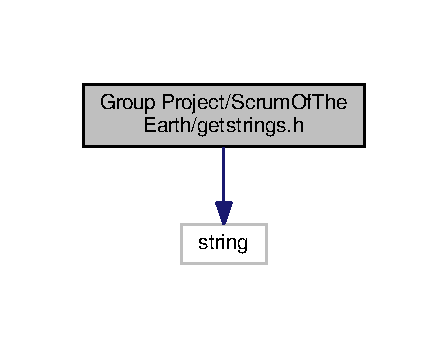
\includegraphics[width=215pt]{getstrings_8h__incl}
\end{center}
\end{figure}
This graph shows which files directly or indirectly include this file\+:\nopagebreak
\begin{figure}[H]
\begin{center}
\leavevmode
\includegraphics[width=350pt]{getstrings_8h__dep__incl}
\end{center}
\end{figure}
\subsection*{Functions}
\begin{DoxyCompactItemize}
\item 
std\+::string \hyperlink{getstrings_8h_ae2e8c725725c53aced4754efb1ba3297}{get\+Pen\+Style} (int ps)
\begin{DoxyCompactList}\small\item\em Converts an index to a string for a penstyle. \end{DoxyCompactList}\item 
std\+::string \hyperlink{getstrings_8h_a36f20d2b33b32e3051b9439984fa3dc1}{get\+Color} (int color)
\begin{DoxyCompactList}\small\item\em Converts an index to a string for a color. \end{DoxyCompactList}\item 
std\+::string \hyperlink{getstrings_8h_ab55986fc16e82140cc960949e8d98fc3}{get\+Pen\+Cap\+Style} (int pcs)
\begin{DoxyCompactList}\small\item\em Converts an index to a string for a pen cap style. \end{DoxyCompactList}\item 
std\+::string \hyperlink{getstrings_8h_a59c542c498dce52daab6c95e393084f7}{get\+Pen\+Join\+Style} (int pjs)
\begin{DoxyCompactList}\small\item\em Converts an index to a string for a pen join style. \end{DoxyCompactList}\item 
std\+::string \hyperlink{getstrings_8h_a59572458de7eabcb211b12647cd8cc67}{get\+Brush\+Style} (int bs)
\begin{DoxyCompactList}\small\item\em Converts an index to a string for a brush style. \end{DoxyCompactList}\item 
std\+::string \hyperlink{getstrings_8h_ab73fa4f5c93f8a3c34cc0a3aaf7508d8}{get\+Text\+Alignment} (int ta)
\begin{DoxyCompactList}\small\item\em Converts an index to a string for a text alignment. \end{DoxyCompactList}\item 
std\+::string \hyperlink{getstrings_8h_a362dd7a8956d7364df5cce0070ec15ca}{get\+Font\+Style} (int fs)
\begin{DoxyCompactList}\small\item\em Converts an index to a string for a font style. \end{DoxyCompactList}\item 
std\+::string \hyperlink{getstrings_8h_a4d2ad0fcdf9ccdd1fdb8f8da293f051d}{get\+Font\+Weight} (int fw)
\begin{DoxyCompactList}\small\item\em Converts an index to a string for font weight. \end{DoxyCompactList}\end{DoxyCompactItemize}


\subsection{Function Documentation}
\index{getstrings.\+h@{getstrings.\+h}!get\+Brush\+Style@{get\+Brush\+Style}}
\index{get\+Brush\+Style@{get\+Brush\+Style}!getstrings.\+h@{getstrings.\+h}}
\subsubsection[{\texorpdfstring{get\+Brush\+Style(int bs)}{getBrushStyle(int bs)}}]{\setlength{\rightskip}{0pt plus 5cm}std\+::string get\+Brush\+Style (
\begin{DoxyParamCaption}
\item[{int}]{bs}
\end{DoxyParamCaption}
)}\hypertarget{getstrings_8h_a59572458de7eabcb211b12647cd8cc67}{}\label{getstrings_8h_a59572458de7eabcb211b12647cd8cc67}


Converts an index to a string for a brush style. 


\begin{DoxyParams}{Parameters}
{\em index} & for brush style \\
\hline
\end{DoxyParams}
\begin{DoxyReturn}{Returns}
string for brush style 
\end{DoxyReturn}
\index{getstrings.\+h@{getstrings.\+h}!get\+Color@{get\+Color}}
\index{get\+Color@{get\+Color}!getstrings.\+h@{getstrings.\+h}}
\subsubsection[{\texorpdfstring{get\+Color(int color)}{getColor(int color)}}]{\setlength{\rightskip}{0pt plus 5cm}std\+::string get\+Color (
\begin{DoxyParamCaption}
\item[{int}]{color}
\end{DoxyParamCaption}
)}\hypertarget{getstrings_8h_a36f20d2b33b32e3051b9439984fa3dc1}{}\label{getstrings_8h_a36f20d2b33b32e3051b9439984fa3dc1}


Converts an index to a string for a color. 


\begin{DoxyParams}{Parameters}
{\em index} & for color \\
\hline
\end{DoxyParams}
\begin{DoxyReturn}{Returns}
string for color 
\end{DoxyReturn}
\index{getstrings.\+h@{getstrings.\+h}!get\+Font\+Style@{get\+Font\+Style}}
\index{get\+Font\+Style@{get\+Font\+Style}!getstrings.\+h@{getstrings.\+h}}
\subsubsection[{\texorpdfstring{get\+Font\+Style(int fs)}{getFontStyle(int fs)}}]{\setlength{\rightskip}{0pt plus 5cm}std\+::string get\+Font\+Style (
\begin{DoxyParamCaption}
\item[{int}]{fs}
\end{DoxyParamCaption}
)}\hypertarget{getstrings_8h_a362dd7a8956d7364df5cce0070ec15ca}{}\label{getstrings_8h_a362dd7a8956d7364df5cce0070ec15ca}


Converts an index to a string for a font style. 


\begin{DoxyParams}{Parameters}
{\em index} & for font style \\
\hline
\end{DoxyParams}
\begin{DoxyReturn}{Returns}
string for font style 
\end{DoxyReturn}
\index{getstrings.\+h@{getstrings.\+h}!get\+Font\+Weight@{get\+Font\+Weight}}
\index{get\+Font\+Weight@{get\+Font\+Weight}!getstrings.\+h@{getstrings.\+h}}
\subsubsection[{\texorpdfstring{get\+Font\+Weight(int fw)}{getFontWeight(int fw)}}]{\setlength{\rightskip}{0pt plus 5cm}std\+::string get\+Font\+Weight (
\begin{DoxyParamCaption}
\item[{int}]{fw}
\end{DoxyParamCaption}
)}\hypertarget{getstrings_8h_a4d2ad0fcdf9ccdd1fdb8f8da293f051d}{}\label{getstrings_8h_a4d2ad0fcdf9ccdd1fdb8f8da293f051d}


Converts an index to a string for font weight. 


\begin{DoxyParams}{Parameters}
{\em index} & for font weight \\
\hline
\end{DoxyParams}
\begin{DoxyReturn}{Returns}
string for font weight 
\end{DoxyReturn}
\index{getstrings.\+h@{getstrings.\+h}!get\+Pen\+Cap\+Style@{get\+Pen\+Cap\+Style}}
\index{get\+Pen\+Cap\+Style@{get\+Pen\+Cap\+Style}!getstrings.\+h@{getstrings.\+h}}
\subsubsection[{\texorpdfstring{get\+Pen\+Cap\+Style(int pcs)}{getPenCapStyle(int pcs)}}]{\setlength{\rightskip}{0pt plus 5cm}std\+::string get\+Pen\+Cap\+Style (
\begin{DoxyParamCaption}
\item[{int}]{pcs}
\end{DoxyParamCaption}
)}\hypertarget{getstrings_8h_ab55986fc16e82140cc960949e8d98fc3}{}\label{getstrings_8h_ab55986fc16e82140cc960949e8d98fc3}


Converts an index to a string for a pen cap style. 


\begin{DoxyParams}{Parameters}
{\em index} & for pen cap style \\
\hline
\end{DoxyParams}
\begin{DoxyReturn}{Returns}
string for pen cap style 
\end{DoxyReturn}
\index{getstrings.\+h@{getstrings.\+h}!get\+Pen\+Join\+Style@{get\+Pen\+Join\+Style}}
\index{get\+Pen\+Join\+Style@{get\+Pen\+Join\+Style}!getstrings.\+h@{getstrings.\+h}}
\subsubsection[{\texorpdfstring{get\+Pen\+Join\+Style(int pjs)}{getPenJoinStyle(int pjs)}}]{\setlength{\rightskip}{0pt plus 5cm}std\+::string get\+Pen\+Join\+Style (
\begin{DoxyParamCaption}
\item[{int}]{pjs}
\end{DoxyParamCaption}
)}\hypertarget{getstrings_8h_a59c542c498dce52daab6c95e393084f7}{}\label{getstrings_8h_a59c542c498dce52daab6c95e393084f7}


Converts an index to a string for a pen join style. 


\begin{DoxyParams}{Parameters}
{\em index} & for pen join style \\
\hline
\end{DoxyParams}
\begin{DoxyReturn}{Returns}
string for pen join style 
\end{DoxyReturn}
\index{getstrings.\+h@{getstrings.\+h}!get\+Pen\+Style@{get\+Pen\+Style}}
\index{get\+Pen\+Style@{get\+Pen\+Style}!getstrings.\+h@{getstrings.\+h}}
\subsubsection[{\texorpdfstring{get\+Pen\+Style(int ps)}{getPenStyle(int ps)}}]{\setlength{\rightskip}{0pt plus 5cm}std\+::string get\+Pen\+Style (
\begin{DoxyParamCaption}
\item[{int}]{ps}
\end{DoxyParamCaption}
)}\hypertarget{getstrings_8h_ae2e8c725725c53aced4754efb1ba3297}{}\label{getstrings_8h_ae2e8c725725c53aced4754efb1ba3297}


Converts an index to a string for a penstyle. 


\begin{DoxyParams}{Parameters}
{\em index} & for penstyle \\
\hline
\end{DoxyParams}
\begin{DoxyReturn}{Returns}
string of penstyle 
\end{DoxyReturn}
\index{getstrings.\+h@{getstrings.\+h}!get\+Text\+Alignment@{get\+Text\+Alignment}}
\index{get\+Text\+Alignment@{get\+Text\+Alignment}!getstrings.\+h@{getstrings.\+h}}
\subsubsection[{\texorpdfstring{get\+Text\+Alignment(int ta)}{getTextAlignment(int ta)}}]{\setlength{\rightskip}{0pt plus 5cm}std\+::string get\+Text\+Alignment (
\begin{DoxyParamCaption}
\item[{int}]{ta}
\end{DoxyParamCaption}
)}\hypertarget{getstrings_8h_ab73fa4f5c93f8a3c34cc0a3aaf7508d8}{}\label{getstrings_8h_ab73fa4f5c93f8a3c34cc0a3aaf7508d8}


Converts an index to a string for a text alignment. 


\begin{DoxyParams}{Parameters}
{\em index} & for text alignment \\
\hline
\end{DoxyParams}
\begin{DoxyReturn}{Returns}
string for text alignment 
\end{DoxyReturn}

\hypertarget{line_8cpp}{}\section{Group Project/\+Scrum\+Of\+The\+Earth/line.cpp File Reference}
\label{line_8cpp}\index{Group Project/\+Scrum\+Of\+The\+Earth/line.\+cpp@{Group Project/\+Scrum\+Of\+The\+Earth/line.\+cpp}}
{\ttfamily \#include \char`\"{}line.\+h\char`\"{}}\\*
Include dependency graph for line.\+cpp\+:\nopagebreak
\begin{figure}[H]
\begin{center}
\leavevmode
\includegraphics[width=280pt]{line_8cpp__incl}
\end{center}
\end{figure}

\hypertarget{line_8h}{}\section{Group Project/\+Scrum\+Of\+The\+Earth/line.h File Reference}
\label{line_8h}\index{Group Project/\+Scrum\+Of\+The\+Earth/line.\+h@{Group Project/\+Scrum\+Of\+The\+Earth/line.\+h}}
{\ttfamily \#include \char`\"{}shape.\+h\char`\"{}}\\*
{\ttfamily \#include $<$cmath$>$}\\*
Include dependency graph for line.\+h\+:\nopagebreak
\begin{figure}[H]
\begin{center}
\leavevmode
\includegraphics[width=280pt]{line_8h__incl}
\end{center}
\end{figure}
This graph shows which files directly or indirectly include this file\+:\nopagebreak
\begin{figure}[H]
\begin{center}
\leavevmode
\includegraphics[width=350pt]{line_8h__dep__incl}
\end{center}
\end{figure}
\subsection*{Classes}
\begin{DoxyCompactItemize}
\item 
class \hyperlink{classLine}{Line}
\begin{DoxyCompactList}\small\item\em \hyperlink{classLine}{Line} class that Q\+Painter can draw. \end{DoxyCompactList}\end{DoxyCompactItemize}

\hypertarget{main_8cpp}{}\section{Group Project/\+Scrum\+Of\+The\+Earth/main.cpp File Reference}
\label{main_8cpp}\index{Group Project/\+Scrum\+Of\+The\+Earth/main.\+cpp@{Group Project/\+Scrum\+Of\+The\+Earth/main.\+cpp}}
{\ttfamily \#include \char`\"{}window.\+h\char`\"{}}\\*
{\ttfamily \#include $<$Q\+Application$>$}\\*
{\ttfamily \#include $<$iostream$>$}\\*
{\ttfamily \#include $<$fstream$>$}\\*
{\ttfamily \#include $<$string$>$}\\*
{\ttfamily \#include $<$sstream$>$}\\*
Include dependency graph for main.\+cpp\+:\nopagebreak
\begin{figure}[H]
\begin{center}
\leavevmode
\includegraphics[width=350pt]{main_8cpp__incl}
\end{center}
\end{figure}
\subsection*{Functions}
\begin{DoxyCompactItemize}
\item 
int \hyperlink{main_8cpp_a0ddf1224851353fc92bfbff6f499fa97}{main} (int argc, char $\ast$argv\mbox{[}$\,$\mbox{]})
\begin{DoxyCompactList}\small\item\em main entry point for program \end{DoxyCompactList}\end{DoxyCompactItemize}


\subsection{Function Documentation}
\index{main.\+cpp@{main.\+cpp}!main@{main}}
\index{main@{main}!main.\+cpp@{main.\+cpp}}
\subsubsection[{\texorpdfstring{main(int argc, char $\ast$argv[])}{main(int argc, char *argv[])}}]{\setlength{\rightskip}{0pt plus 5cm}int main (
\begin{DoxyParamCaption}
\item[{int}]{argc, }
\item[{char $\ast$}]{argv\mbox{[}$\,$\mbox{]}}
\end{DoxyParamCaption}
)}\hypertarget{main_8cpp_a0ddf1224851353fc92bfbff6f499fa97}{}\label{main_8cpp_a0ddf1224851353fc92bfbff6f499fa97}


main entry point for program 


\begin{DoxyParams}{Parameters}
{\em argc} & number of arguments \\
\hline
{\em argv} & arguments as cstrings \\
\hline
\end{DoxyParams}
\begin{DoxyReturn}{Returns}

\end{DoxyReturn}

\hypertarget{mainwindow_8cpp}{}\section{Group Project/\+Scrum\+Of\+The\+Earth/mainwindow.cpp File Reference}
\label{mainwindow_8cpp}\index{Group Project/\+Scrum\+Of\+The\+Earth/mainwindow.\+cpp@{Group Project/\+Scrum\+Of\+The\+Earth/mainwindow.\+cpp}}
{\ttfamily \#include \char`\"{}mainwindow.\+h\char`\"{}}\\*
{\ttfamily \#include \char`\"{}ui\+\_\+mainwindow.\+h\char`\"{}}\\*
{\ttfamily \#include $<$Q\+Input\+Dialog$>$}\\*
{\ttfamily \#include \char`\"{}shape.\+h\char`\"{}}\\*
{\ttfamily \#include \char`\"{}square.\+h\char`\"{}}\\*
{\ttfamily \#include \char`\"{}circle.\+h\char`\"{}}\\*
{\ttfamily \#include \char`\"{}ellipse.\+h\char`\"{}}\\*
{\ttfamily \#include \char`\"{}polygon.\+h\char`\"{}}\\*
{\ttfamily \#include \char`\"{}polyline.\+h\char`\"{}}\\*
{\ttfamily \#include \char`\"{}line.\+h\char`\"{}}\\*
{\ttfamily \#include $<$Q\+Point$>$}\\*
{\ttfamily \#include \char`\"{}shape\+\_\+parser.\+h\char`\"{}}\\*
{\ttfamily \#include $<$Q\+Message\+Box$>$}\\*
{\ttfamily \#include \char`\"{}searchandcompare.\+h\char`\"{}}\\*
{\ttfamily \#include \char`\"{}pop\+\_\+table.\+h\char`\"{}}\\*
{\ttfamily \#include $<$Q\+File\+Dialog$>$}\\*
{\ttfamily \#include \char`\"{}delete\+\_\+zeros.\+h\char`\"{}}\\*
{\ttfamily \#include $<$string$>$}\\*
Include dependency graph for mainwindow.\+cpp\+:\nopagebreak
\begin{figure}[H]
\begin{center}
\leavevmode
\includegraphics[width=350pt]{mainwindow_8cpp__incl}
\end{center}
\end{figure}

\hypertarget{mainwindow_8h}{}\section{Group Project/\+Scrum\+Of\+The\+Earth/mainwindow.h File Reference}
\label{mainwindow_8h}\index{Group Project/\+Scrum\+Of\+The\+Earth/mainwindow.\+h@{Group Project/\+Scrum\+Of\+The\+Earth/mainwindow.\+h}}
{\ttfamily \#include \char`\"{}addshape.\+h\char`\"{}}\\*
{\ttfamily \#include \char`\"{}moveshape.\+h\char`\"{}}\\*
{\ttfamily \#include $<$Q\+Main\+Window$>$}\\*
Include dependency graph for mainwindow.\+h\+:\nopagebreak
\begin{figure}[H]
\begin{center}
\leavevmode
\includegraphics[width=350pt]{mainwindow_8h__incl}
\end{center}
\end{figure}
This graph shows which files directly or indirectly include this file\+:\nopagebreak
\begin{figure}[H]
\begin{center}
\leavevmode
\includegraphics[width=350pt]{mainwindow_8h__dep__incl}
\end{center}
\end{figure}
\subsection*{Classes}
\begin{DoxyCompactItemize}
\item 
class \hyperlink{classMainWindow}{Main\+Window}
\begin{DoxyCompactList}\small\item\em The \hyperlink{classMainWindow}{Main\+Window} class provides the environment for the \hyperlink{classRenderArea}{Render\+Area}, Tables, and Buttons. \end{DoxyCompactList}\end{DoxyCompactItemize}
\subsection*{Namespaces}
\begin{DoxyCompactItemize}
\item 
 \hyperlink{namespaceUi}{Ui}
\end{DoxyCompactItemize}

\hypertarget{moveshape_8cpp}{}\section{Group Project/\+Scrum\+Of\+The\+Earth/moveshape.cpp File Reference}
\label{moveshape_8cpp}\index{Group Project/\+Scrum\+Of\+The\+Earth/moveshape.\+cpp@{Group Project/\+Scrum\+Of\+The\+Earth/moveshape.\+cpp}}
{\ttfamily \#include \char`\"{}moveshape.\+h\char`\"{}}\\*
{\ttfamily \#include \char`\"{}ui\+\_\+moveshape.\+h\char`\"{}}\\*
{\ttfamily \#include $<$iostream$>$}\\*
Include dependency graph for moveshape.\+cpp\+:\nopagebreak
\begin{figure}[H]
\begin{center}
\leavevmode
\includegraphics[width=350pt]{moveshape_8cpp__incl}
\end{center}
\end{figure}

\hypertarget{moveshape_8h}{}\section{Group Project/\+Scrum\+Of\+The\+Earth/moveshape.h File Reference}
\label{moveshape_8h}\index{Group Project/\+Scrum\+Of\+The\+Earth/moveshape.\+h@{Group Project/\+Scrum\+Of\+The\+Earth/moveshape.\+h}}
{\ttfamily \#include \char`\"{}vector.\+h\char`\"{}}\\*
{\ttfamily \#include \char`\"{}shape.\+h\char`\"{}}\\*
{\ttfamily \#include \char`\"{}square.\+h\char`\"{}}\\*
{\ttfamily \#include \char`\"{}rectangle.\+h\char`\"{}}\\*
{\ttfamily \#include \char`\"{}line.\+h\char`\"{}}\\*
{\ttfamily \#include \char`\"{}circle.\+h\char`\"{}}\\*
{\ttfamily \#include \char`\"{}ellipse.\+h\char`\"{}}\\*
{\ttfamily \#include \char`\"{}polygon.\+h\char`\"{}}\\*
{\ttfamily \#include \char`\"{}polyline.\+h\char`\"{}}\\*
{\ttfamily \#include \char`\"{}text.\+h\char`\"{}}\\*
{\ttfamily \#include $<$string$>$}\\*
{\ttfamily \#include $<$Q\+Main\+Window$>$}\\*
Include dependency graph for moveshape.\+h\+:\nopagebreak
\begin{figure}[H]
\begin{center}
\leavevmode
\includegraphics[width=350pt]{moveshape_8h__incl}
\end{center}
\end{figure}
This graph shows which files directly or indirectly include this file\+:\nopagebreak
\begin{figure}[H]
\begin{center}
\leavevmode
\includegraphics[width=350pt]{moveshape_8h__dep__incl}
\end{center}
\end{figure}
\subsection*{Classes}
\begin{DoxyCompactItemize}
\item 
class \hyperlink{classMoveShape}{Move\+Shape}
\begin{DoxyCompactList}\small\item\em The \hyperlink{classMoveShape}{Move\+Shape} class provides the interface and functionality for moving shapes. \end{DoxyCompactList}\end{DoxyCompactItemize}
\subsection*{Namespaces}
\begin{DoxyCompactItemize}
\item 
 \hyperlink{namespaceUi}{Ui}
\end{DoxyCompactItemize}

\hypertarget{polygon_8cpp}{}\section{Group Project/\+Scrum\+Of\+The\+Earth/polygon.cpp File Reference}
\label{polygon_8cpp}\index{Group Project/\+Scrum\+Of\+The\+Earth/polygon.\+cpp@{Group Project/\+Scrum\+Of\+The\+Earth/polygon.\+cpp}}
{\ttfamily \#include \char`\"{}polygon.\+h\char`\"{}}\\*
{\ttfamily \#include $<$iostream$>$}\\*
Include dependency graph for polygon.\+cpp\+:\nopagebreak
\begin{figure}[H]
\begin{center}
\leavevmode
\includegraphics[width=350pt]{polygon_8cpp__incl}
\end{center}
\end{figure}

\hypertarget{polygon_8h}{}\section{Group Project/\+Scrum\+Of\+The\+Earth/polygon.h File Reference}
\label{polygon_8h}\index{Group Project/\+Scrum\+Of\+The\+Earth/polygon.\+h@{Group Project/\+Scrum\+Of\+The\+Earth/polygon.\+h}}
{\ttfamily \#include \char`\"{}shape.\+h\char`\"{}}\\*
{\ttfamily \#include \char`\"{}vector.\+h\char`\"{}}\\*
{\ttfamily \#include $<$cmath$>$}\\*
Include dependency graph for polygon.\+h\+:\nopagebreak
\begin{figure}[H]
\begin{center}
\leavevmode
\includegraphics[width=318pt]{polygon_8h__incl}
\end{center}
\end{figure}
This graph shows which files directly or indirectly include this file\+:\nopagebreak
\begin{figure}[H]
\begin{center}
\leavevmode
\includegraphics[width=350pt]{polygon_8h__dep__incl}
\end{center}
\end{figure}
\subsection*{Classes}
\begin{DoxyCompactItemize}
\item 
class \hyperlink{classPolygon}{Polygon}
\begin{DoxyCompactList}\small\item\em \hyperlink{classPolygon}{Polygon} class that Q\+Painter can draw. \end{DoxyCompactList}\end{DoxyCompactItemize}

\hypertarget{polyline_8cpp}{}\section{Group Project/\+Scrum\+Of\+The\+Earth/polyline.cpp File Reference}
\label{polyline_8cpp}\index{Group Project/\+Scrum\+Of\+The\+Earth/polyline.\+cpp@{Group Project/\+Scrum\+Of\+The\+Earth/polyline.\+cpp}}
{\ttfamily \#include \char`\"{}polyline.\+h\char`\"{}}\\*
{\ttfamily \#include $<$iostream$>$}\\*
Include dependency graph for polyline.\+cpp\+:\nopagebreak
\begin{figure}[H]
\begin{center}
\leavevmode
\includegraphics[width=280pt]{polyline_8cpp__incl}
\end{center}
\end{figure}

\hypertarget{polyline_8h}{}\section{Group Project/\+Scrum\+Of\+The\+Earth/polyline.h File Reference}
\label{polyline_8h}\index{Group Project/\+Scrum\+Of\+The\+Earth/polyline.\+h@{Group Project/\+Scrum\+Of\+The\+Earth/polyline.\+h}}
{\ttfamily \#include \char`\"{}vector.\+h\char`\"{}}\\*
{\ttfamily \#include \char`\"{}shape.\+h\char`\"{}}\\*
{\ttfamily \#include $<$cmath$>$}\\*
Include dependency graph for polyline.\+h\+:\nopagebreak
\begin{figure}[H]
\begin{center}
\leavevmode
\includegraphics[width=279pt]{polyline_8h__incl}
\end{center}
\end{figure}
This graph shows which files directly or indirectly include this file\+:\nopagebreak
\begin{figure}[H]
\begin{center}
\leavevmode
\includegraphics[width=350pt]{polyline_8h__dep__incl}
\end{center}
\end{figure}
\subsection*{Classes}
\begin{DoxyCompactItemize}
\item 
class \hyperlink{classPolyline}{Polyline}
\begin{DoxyCompactList}\small\item\em \hyperlink{classPolyline}{Polyline} class that Q\+Painter can draw. \end{DoxyCompactList}\end{DoxyCompactItemize}

\hypertarget{pop__table_8cpp}{}\section{Group Project/\+Scrum\+Of\+The\+Earth/pop\+\_\+table.cpp File Reference}
\label{pop__table_8cpp}\index{Group Project/\+Scrum\+Of\+The\+Earth/pop\+\_\+table.\+cpp@{Group Project/\+Scrum\+Of\+The\+Earth/pop\+\_\+table.\+cpp}}
{\ttfamily \#include \char`\"{}pop\+\_\+table.\+h\char`\"{}}\\*
{\ttfamily \#include \char`\"{}square.\+h\char`\"{}}\\*
{\ttfamily \#include \char`\"{}rectangle.\+h\char`\"{}}\\*
{\ttfamily \#include \char`\"{}circle.\+h\char`\"{}}\\*
{\ttfamily \#include \char`\"{}ellipse.\+h\char`\"{}}\\*
{\ttfamily \#include \char`\"{}text.\+h\char`\"{}}\\*
{\ttfamily \#include \char`\"{}line.\+h\char`\"{}}\\*
{\ttfamily \#include \char`\"{}polyline.\+h\char`\"{}}\\*
{\ttfamily \#include \char`\"{}polygon.\+h\char`\"{}}\\*
{\ttfamily \#include $<$Q\+String$>$}\\*
{\ttfamily \#include $<$iostream$>$}\\*
{\ttfamily \#include $<$string$>$}\\*
Include dependency graph for pop\+\_\+table.\+cpp\+:\nopagebreak
\begin{figure}[H]
\begin{center}
\leavevmode
\includegraphics[width=350pt]{pop__table_8cpp__incl}
\end{center}
\end{figure}
\subsection*{Functions}
\begin{DoxyCompactItemize}
\item 
void \hyperlink{pop__table_8cpp_ada07240decd2206bb697cd31dd579839}{pop\+\_\+\+Atable} (Q\+Table\+Widget $\ast$tble, \hyperlink{classmyStd_1_1vector}{my\+Std\+::vector}$<$ \hyperlink{classShape}{Shape} $\ast$ $>$ vec)
\begin{DoxyCompactList}\small\item\em pop\+\_\+\+Atable populates a given table with shape types, ids, and areas from a vector of \hyperlink{classShape}{Shape} pointers \end{DoxyCompactList}\item 
void \hyperlink{pop__table_8cpp_ad8d8a27f7ccd50e0c6c9173f37c2b8fd}{pop\+\_\+\+Ptable} (Q\+Table\+Widget $\ast$tble, \hyperlink{classmyStd_1_1vector}{my\+Std\+::vector}$<$ \hyperlink{classShape}{Shape} $\ast$ $>$ vec)
\begin{DoxyCompactList}\small\item\em pop\+\_\+\+Ptable populates a given table with shape types, ids, and perimeters from a vector of \hyperlink{classShape}{Shape} pointers \end{DoxyCompactList}\item 
void \hyperlink{pop__table_8cpp_a7e4b678b55853077d6514112c661d121}{fill\+\_\+table} (Q\+Table\+Widget $\ast$tble, \hyperlink{classmyStd_1_1vector}{my\+Std\+::vector}$<$ \hyperlink{classShape}{Shape} $\ast$ $>$ vec)
\begin{DoxyCompactList}\small\item\em fill\+\_\+table populates a given table with all aspects of the Shapes form a vector of \hyperlink{classShape}{Shape} pointers \end{DoxyCompactList}\end{DoxyCompactItemize}


\subsection{Function Documentation}
\index{pop\+\_\+table.\+cpp@{pop\+\_\+table.\+cpp}!fill\+\_\+table@{fill\+\_\+table}}
\index{fill\+\_\+table@{fill\+\_\+table}!pop\+\_\+table.\+cpp@{pop\+\_\+table.\+cpp}}
\subsubsection[{\texorpdfstring{fill\+\_\+table(\+Q\+Table\+Widget $\ast$tble, my\+Std\+::vector$<$ Shape $\ast$ $>$ vec)}{fill_table(QTableWidget *tble, myStd::vector< Shape * > vec)}}]{\setlength{\rightskip}{0pt plus 5cm}void fill\+\_\+table (
\begin{DoxyParamCaption}
\item[{Q\+Table\+Widget $\ast$}]{tble, }
\item[{{\bf my\+Std\+::vector}$<$ {\bf Shape} $\ast$ $>$}]{vec}
\end{DoxyParamCaption}
)}\hypertarget{pop__table_8cpp_a7e4b678b55853077d6514112c661d121}{}\label{pop__table_8cpp_a7e4b678b55853077d6514112c661d121}


fill\+\_\+table populates a given table with all aspects of the Shapes form a vector of \hyperlink{classShape}{Shape} pointers 

\index{pop\+\_\+table.\+cpp@{pop\+\_\+table.\+cpp}!pop\+\_\+\+Atable@{pop\+\_\+\+Atable}}
\index{pop\+\_\+\+Atable@{pop\+\_\+\+Atable}!pop\+\_\+table.\+cpp@{pop\+\_\+table.\+cpp}}
\subsubsection[{\texorpdfstring{pop\+\_\+\+Atable(\+Q\+Table\+Widget $\ast$tble, my\+Std\+::vector$<$ Shape $\ast$ $>$ vec)}{pop_Atable(QTableWidget *tble, myStd::vector< Shape * > vec)}}]{\setlength{\rightskip}{0pt plus 5cm}void pop\+\_\+\+Atable (
\begin{DoxyParamCaption}
\item[{Q\+Table\+Widget $\ast$}]{tble, }
\item[{{\bf my\+Std\+::vector}$<$ {\bf Shape} $\ast$ $>$}]{vec}
\end{DoxyParamCaption}
)}\hypertarget{pop__table_8cpp_ada07240decd2206bb697cd31dd579839}{}\label{pop__table_8cpp_ada07240decd2206bb697cd31dd579839}


pop\+\_\+\+Atable populates a given table with shape types, ids, and areas from a vector of \hyperlink{classShape}{Shape} pointers 

\index{pop\+\_\+table.\+cpp@{pop\+\_\+table.\+cpp}!pop\+\_\+\+Ptable@{pop\+\_\+\+Ptable}}
\index{pop\+\_\+\+Ptable@{pop\+\_\+\+Ptable}!pop\+\_\+table.\+cpp@{pop\+\_\+table.\+cpp}}
\subsubsection[{\texorpdfstring{pop\+\_\+\+Ptable(\+Q\+Table\+Widget $\ast$tble, my\+Std\+::vector$<$ Shape $\ast$ $>$ vec)}{pop_Ptable(QTableWidget *tble, myStd::vector< Shape * > vec)}}]{\setlength{\rightskip}{0pt plus 5cm}void pop\+\_\+\+Ptable (
\begin{DoxyParamCaption}
\item[{Q\+Table\+Widget $\ast$}]{tble, }
\item[{{\bf my\+Std\+::vector}$<$ {\bf Shape} $\ast$ $>$}]{vec}
\end{DoxyParamCaption}
)}\hypertarget{pop__table_8cpp_ad8d8a27f7ccd50e0c6c9173f37c2b8fd}{}\label{pop__table_8cpp_ad8d8a27f7ccd50e0c6c9173f37c2b8fd}


pop\+\_\+\+Ptable populates a given table with shape types, ids, and perimeters from a vector of \hyperlink{classShape}{Shape} pointers 


\hypertarget{pop__table_8h}{}\section{Group Project/\+Scrum\+Of\+The\+Earth/pop\+\_\+table.h File Reference}
\label{pop__table_8h}\index{Group Project/\+Scrum\+Of\+The\+Earth/pop\+\_\+table.\+h@{Group Project/\+Scrum\+Of\+The\+Earth/pop\+\_\+table.\+h}}
{\ttfamily \#include \char`\"{}vector.\+h\char`\"{}}\\*
{\ttfamily \#include $<$Q\+Table\+Widget$>$}\\*
{\ttfamily \#include \char`\"{}shape.\+h\char`\"{}}\\*
Include dependency graph for pop\+\_\+table.\+h\+:\nopagebreak
\begin{figure}[H]
\begin{center}
\leavevmode
\includegraphics[width=301pt]{pop__table_8h__incl}
\end{center}
\end{figure}
This graph shows which files directly or indirectly include this file\+:\nopagebreak
\begin{figure}[H]
\begin{center}
\leavevmode
\includegraphics[width=350pt]{pop__table_8h__dep__incl}
\end{center}
\end{figure}
\subsection*{Functions}
\begin{DoxyCompactItemize}
\item 
void \hyperlink{pop__table_8h_a7cfa9abf76a3ab65ebd5506ad1ee21f2}{pop\+\_\+\+Atable} (Q\+Table\+Widget $\ast$, \hyperlink{classmyStd_1_1vector}{my\+Std\+::vector}$<$ \hyperlink{classShape}{Shape} $\ast$ $>$)
\begin{DoxyCompactList}\small\item\em pop\+\_\+\+Atable populates a given table with shape types, ids, and areas from a vector of \hyperlink{classShape}{Shape} pointers \end{DoxyCompactList}\item 
void \hyperlink{pop__table_8h_a3a41a87f334ddb881f4532c8080f7101}{pop\+\_\+\+Ptable} (Q\+Table\+Widget $\ast$, \hyperlink{classmyStd_1_1vector}{my\+Std\+::vector}$<$ \hyperlink{classShape}{Shape} $\ast$ $>$)
\begin{DoxyCompactList}\small\item\em pop\+\_\+\+Ptable populates a given table with shape types, ids, and perimeters from a vector of \hyperlink{classShape}{Shape} pointers \end{DoxyCompactList}\item 
void \hyperlink{pop__table_8h_a6f42cb3c5185e6fdaf9c12c620c5b87f}{fill\+\_\+table} (Q\+Table\+Widget $\ast$, \hyperlink{classmyStd_1_1vector}{my\+Std\+::vector}$<$ \hyperlink{classShape}{Shape} $\ast$ $>$)
\begin{DoxyCompactList}\small\item\em fill\+\_\+table populates a given table with all aspects of the Shapes form a vector of \hyperlink{classShape}{Shape} pointers \end{DoxyCompactList}\end{DoxyCompactItemize}


\subsection{Function Documentation}
\index{pop\+\_\+table.\+h@{pop\+\_\+table.\+h}!fill\+\_\+table@{fill\+\_\+table}}
\index{fill\+\_\+table@{fill\+\_\+table}!pop\+\_\+table.\+h@{pop\+\_\+table.\+h}}
\subsubsection[{\texorpdfstring{fill\+\_\+table(\+Q\+Table\+Widget $\ast$, my\+Std\+::vector$<$ Shape $\ast$ $>$)}{fill_table(QTableWidget *, myStd::vector< Shape * >)}}]{\setlength{\rightskip}{0pt plus 5cm}void fill\+\_\+table (
\begin{DoxyParamCaption}
\item[{Q\+Table\+Widget $\ast$}]{, }
\item[{{\bf my\+Std\+::vector}$<$ {\bf Shape} $\ast$ $>$}]{}
\end{DoxyParamCaption}
)}\hypertarget{pop__table_8h_a6f42cb3c5185e6fdaf9c12c620c5b87f}{}\label{pop__table_8h_a6f42cb3c5185e6fdaf9c12c620c5b87f}


fill\+\_\+table populates a given table with all aspects of the Shapes form a vector of \hyperlink{classShape}{Shape} pointers 

\index{pop\+\_\+table.\+h@{pop\+\_\+table.\+h}!pop\+\_\+\+Atable@{pop\+\_\+\+Atable}}
\index{pop\+\_\+\+Atable@{pop\+\_\+\+Atable}!pop\+\_\+table.\+h@{pop\+\_\+table.\+h}}
\subsubsection[{\texorpdfstring{pop\+\_\+\+Atable(\+Q\+Table\+Widget $\ast$, my\+Std\+::vector$<$ Shape $\ast$ $>$)}{pop_Atable(QTableWidget *, myStd::vector< Shape * >)}}]{\setlength{\rightskip}{0pt plus 5cm}void pop\+\_\+\+Atable (
\begin{DoxyParamCaption}
\item[{Q\+Table\+Widget $\ast$}]{, }
\item[{{\bf my\+Std\+::vector}$<$ {\bf Shape} $\ast$ $>$}]{}
\end{DoxyParamCaption}
)}\hypertarget{pop__table_8h_a7cfa9abf76a3ab65ebd5506ad1ee21f2}{}\label{pop__table_8h_a7cfa9abf76a3ab65ebd5506ad1ee21f2}


pop\+\_\+\+Atable populates a given table with shape types, ids, and areas from a vector of \hyperlink{classShape}{Shape} pointers 

\index{pop\+\_\+table.\+h@{pop\+\_\+table.\+h}!pop\+\_\+\+Ptable@{pop\+\_\+\+Ptable}}
\index{pop\+\_\+\+Ptable@{pop\+\_\+\+Ptable}!pop\+\_\+table.\+h@{pop\+\_\+table.\+h}}
\subsubsection[{\texorpdfstring{pop\+\_\+\+Ptable(\+Q\+Table\+Widget $\ast$, my\+Std\+::vector$<$ Shape $\ast$ $>$)}{pop_Ptable(QTableWidget *, myStd::vector< Shape * >)}}]{\setlength{\rightskip}{0pt plus 5cm}void pop\+\_\+\+Ptable (
\begin{DoxyParamCaption}
\item[{Q\+Table\+Widget $\ast$}]{, }
\item[{{\bf my\+Std\+::vector}$<$ {\bf Shape} $\ast$ $>$}]{}
\end{DoxyParamCaption}
)}\hypertarget{pop__table_8h_a3a41a87f334ddb881f4532c8080f7101}{}\label{pop__table_8h_a3a41a87f334ddb881f4532c8080f7101}


pop\+\_\+\+Ptable populates a given table with shape types, ids, and perimeters from a vector of \hyperlink{classShape}{Shape} pointers 


\hypertarget{rectangle_8cpp}{}\section{Group Project/\+Scrum\+Of\+The\+Earth/rectangle.cpp File Reference}
\label{rectangle_8cpp}\index{Group Project/\+Scrum\+Of\+The\+Earth/rectangle.\+cpp@{Group Project/\+Scrum\+Of\+The\+Earth/rectangle.\+cpp}}
{\ttfamily \#include \char`\"{}rectangle.\+h\char`\"{}}\\*
Include dependency graph for rectangle.\+cpp\+:\nopagebreak
\begin{figure}[H]
\begin{center}
\leavevmode
\includegraphics[width=282pt]{rectangle_8cpp__incl}
\end{center}
\end{figure}

\hypertarget{rectangle_8h}{}\section{Group Project/\+Scrum\+Of\+The\+Earth/rectangle.h File Reference}
\label{rectangle_8h}\index{Group Project/\+Scrum\+Of\+The\+Earth/rectangle.\+h@{Group Project/\+Scrum\+Of\+The\+Earth/rectangle.\+h}}
{\ttfamily \#include \char`\"{}shape.\+h\char`\"{}}\\*
{\ttfamily \#include \char`\"{}vector.\+h\char`\"{}}\\*
Include dependency graph for rectangle.\+h\+:\nopagebreak
\begin{figure}[H]
\begin{center}
\leavevmode
\includegraphics[width=282pt]{rectangle_8h__incl}
\end{center}
\end{figure}
This graph shows which files directly or indirectly include this file\+:\nopagebreak
\begin{figure}[H]
\begin{center}
\leavevmode
\includegraphics[width=350pt]{rectangle_8h__dep__incl}
\end{center}
\end{figure}
\subsection*{Classes}
\begin{DoxyCompactItemize}
\item 
class \hyperlink{classRectangle}{Rectangle}
\begin{DoxyCompactList}\small\item\em \hyperlink{classRectangle}{Rectangle} class that Q\+Painter can draw. \end{DoxyCompactList}\end{DoxyCompactItemize}

\hypertarget{renderarea_8h}{}\section{Group Project/\+Scrum\+Of\+The\+Earth/renderarea.h File Reference}
\label{renderarea_8h}\index{Group Project/\+Scrum\+Of\+The\+Earth/renderarea.\+h@{Group Project/\+Scrum\+Of\+The\+Earth/renderarea.\+h}}
{\ttfamily \#include $<$Q\+Widget$>$}\\*
{\ttfamily \#include \char`\"{}shape.\+h\char`\"{}}\\*
{\ttfamily \#include \char`\"{}vector.\+h\char`\"{}}\\*
{\ttfamily \#include $<$iostream$>$}\\*
Include dependency graph for renderarea.\+h\+:\nopagebreak
\begin{figure}[H]
\begin{center}
\leavevmode
\includegraphics[width=324pt]{renderarea_8h__incl}
\end{center}
\end{figure}
\subsection*{Classes}
\begin{DoxyCompactItemize}
\item 
class \hyperlink{classRenderArea}{Render\+Area}
\begin{DoxyCompactList}\small\item\em The \hyperlink{classRenderArea}{Render\+Area} class provides the environment for drawing shapes. \end{DoxyCompactList}\end{DoxyCompactItemize}

\hypertarget{searchandcompare_8cpp}{}\section{Group Project/\+Scrum\+Of\+The\+Earth/searchandcompare.cpp File Reference}
\label{searchandcompare_8cpp}\index{Group Project/\+Scrum\+Of\+The\+Earth/searchandcompare.\+cpp@{Group Project/\+Scrum\+Of\+The\+Earth/searchandcompare.\+cpp}}
{\ttfamily \#include \char`\"{}searchandcompare.\+h\char`\"{}}\\*
Include dependency graph for searchandcompare.\+cpp\+:\nopagebreak
\begin{figure}[H]
\begin{center}
\leavevmode
\includegraphics[width=288pt]{searchandcompare_8cpp__incl}
\end{center}
\end{figure}
\subsection*{Functions}
\begin{DoxyCompactItemize}
\item 
bool \hyperlink{searchandcompare_8cpp_a474fd352edcedaea9235d8708336d6e0}{cmp\+Id} (\hyperlink{classShape}{Shape} $\ast$s1, \hyperlink{classShape}{Shape} $\ast$s2)
\begin{DoxyCompactList}\small\item\em cmp\+Id compares the id of two shapes and returns true if the id of the first shape is greater. Otherwise, false \end{DoxyCompactList}\item 
bool \hyperlink{searchandcompare_8cpp_a55d382d6ff217cba8f8a1d647d3f5e02}{cmp\+Area} (\hyperlink{classShape}{Shape} $\ast$s1, \hyperlink{classShape}{Shape} $\ast$s2)
\begin{DoxyCompactList}\small\item\em cmp\+Area compares the area of two shapes and returns true if the area of the first shape is greater. Otherwise, false \end{DoxyCompactList}\item 
bool \hyperlink{searchandcompare_8cpp_ab91f3b00a32d9f439cecf4f29ce6eb29}{cmp\+Peri} (\hyperlink{classShape}{Shape} $\ast$s1, \hyperlink{classShape}{Shape} $\ast$s2)
\begin{DoxyCompactList}\small\item\em cmp\+Peri compares the perimeter of two shapes and returns true if the perimeter of the first shape is greater. Otherwise, false \end{DoxyCompactList}\item 
int \hyperlink{searchandcompare_8cpp_ae156afea82af96484e6d6f00195737aa}{find\+Shape} (\hyperlink{classmyStd_1_1vector}{my\+Std\+::vector}$<$ \hyperlink{classShape}{Shape} $\ast$ $>$ vec, unsigned int id)
\begin{DoxyCompactList}\small\item\em find\+Shape finds a shape with the given id in the given vector of shape pointers \end{DoxyCompactList}\end{DoxyCompactItemize}


\subsection{Function Documentation}
\index{searchandcompare.\+cpp@{searchandcompare.\+cpp}!cmp\+Area@{cmp\+Area}}
\index{cmp\+Area@{cmp\+Area}!searchandcompare.\+cpp@{searchandcompare.\+cpp}}
\subsubsection[{\texorpdfstring{cmp\+Area(\+Shape $\ast$s1, Shape $\ast$s2)}{cmpArea(Shape *s1, Shape *s2)}}]{\setlength{\rightskip}{0pt plus 5cm}bool cmp\+Area (
\begin{DoxyParamCaption}
\item[{{\bf Shape} $\ast$}]{s1, }
\item[{{\bf Shape} $\ast$}]{s2}
\end{DoxyParamCaption}
)}\hypertarget{searchandcompare_8cpp_a55d382d6ff217cba8f8a1d647d3f5e02}{}\label{searchandcompare_8cpp_a55d382d6ff217cba8f8a1d647d3f5e02}


cmp\+Area compares the area of two shapes and returns true if the area of the first shape is greater. Otherwise, false 


\begin{DoxyParams}{Parameters}
{\em s1} & \hyperlink{classShape}{Shape} 1 \\
\hline
{\em s2} & \hyperlink{classShape}{Shape} 2 \\
\hline
\end{DoxyParams}
\begin{DoxyReturn}{Returns}
bool \hyperlink{classShape}{Shape} 1\textquotesingle{}s perimeter is greater or not 
\end{DoxyReturn}
\index{searchandcompare.\+cpp@{searchandcompare.\+cpp}!cmp\+Id@{cmp\+Id}}
\index{cmp\+Id@{cmp\+Id}!searchandcompare.\+cpp@{searchandcompare.\+cpp}}
\subsubsection[{\texorpdfstring{cmp\+Id(\+Shape $\ast$s1, Shape $\ast$s2)}{cmpId(Shape *s1, Shape *s2)}}]{\setlength{\rightskip}{0pt plus 5cm}bool cmp\+Id (
\begin{DoxyParamCaption}
\item[{{\bf Shape} $\ast$}]{s1, }
\item[{{\bf Shape} $\ast$}]{s2}
\end{DoxyParamCaption}
)}\hypertarget{searchandcompare_8cpp_a474fd352edcedaea9235d8708336d6e0}{}\label{searchandcompare_8cpp_a474fd352edcedaea9235d8708336d6e0}


cmp\+Id compares the id of two shapes and returns true if the id of the first shape is greater. Otherwise, false 


\begin{DoxyParams}{Parameters}
{\em s1} & \hyperlink{classShape}{Shape} 1 \\
\hline
{\em s2} & \hyperlink{classShape}{Shape} 2 \\
\hline
\end{DoxyParams}
\begin{DoxyReturn}{Returns}
bool \hyperlink{classShape}{Shape} 1\textquotesingle{}s id is greater or not 
\end{DoxyReturn}
\index{searchandcompare.\+cpp@{searchandcompare.\+cpp}!cmp\+Peri@{cmp\+Peri}}
\index{cmp\+Peri@{cmp\+Peri}!searchandcompare.\+cpp@{searchandcompare.\+cpp}}
\subsubsection[{\texorpdfstring{cmp\+Peri(\+Shape $\ast$s1, Shape $\ast$s2)}{cmpPeri(Shape *s1, Shape *s2)}}]{\setlength{\rightskip}{0pt plus 5cm}bool cmp\+Peri (
\begin{DoxyParamCaption}
\item[{{\bf Shape} $\ast$}]{s1, }
\item[{{\bf Shape} $\ast$}]{s2}
\end{DoxyParamCaption}
)}\hypertarget{searchandcompare_8cpp_ab91f3b00a32d9f439cecf4f29ce6eb29}{}\label{searchandcompare_8cpp_ab91f3b00a32d9f439cecf4f29ce6eb29}


cmp\+Peri compares the perimeter of two shapes and returns true if the perimeter of the first shape is greater. Otherwise, false 


\begin{DoxyParams}{Parameters}
{\em s1} & \hyperlink{classShape}{Shape} 1 \\
\hline
{\em s2} & \hyperlink{classShape}{Shape} 2 \\
\hline
\end{DoxyParams}
\begin{DoxyReturn}{Returns}
bool \hyperlink{classShape}{Shape} 1\textquotesingle{}s perimeter is greater or not 
\end{DoxyReturn}
\index{searchandcompare.\+cpp@{searchandcompare.\+cpp}!find\+Shape@{find\+Shape}}
\index{find\+Shape@{find\+Shape}!searchandcompare.\+cpp@{searchandcompare.\+cpp}}
\subsubsection[{\texorpdfstring{find\+Shape(my\+Std\+::vector$<$ Shape $\ast$ $>$ vec, unsigned int id)}{findShape(myStd::vector< Shape * > vec, unsigned int id)}}]{\setlength{\rightskip}{0pt plus 5cm}int find\+Shape (
\begin{DoxyParamCaption}
\item[{{\bf my\+Std\+::vector}$<$ {\bf Shape} $\ast$ $>$}]{, }
\item[{unsigned}]{int}
\end{DoxyParamCaption}
)}\hypertarget{searchandcompare_8cpp_ae156afea82af96484e6d6f00195737aa}{}\label{searchandcompare_8cpp_ae156afea82af96484e6d6f00195737aa}


find\+Shape finds a shape with the given id in the given vector of shape pointers 

\begin{DoxyReturn}{Returns}

\end{DoxyReturn}

\hypertarget{searchandcompare_8h}{}\section{Group Project/\+Scrum\+Of\+The\+Earth/searchandcompare.h File Reference}
\label{searchandcompare_8h}\index{Group Project/\+Scrum\+Of\+The\+Earth/searchandcompare.\+h@{Group Project/\+Scrum\+Of\+The\+Earth/searchandcompare.\+h}}
{\ttfamily \#include \char`\"{}vector.\+h\char`\"{}}\\*
{\ttfamily \#include \char`\"{}shape.\+h\char`\"{}}\\*
Include dependency graph for searchandcompare.\+h\+:\nopagebreak
\begin{figure}[H]
\begin{center}
\leavevmode
\includegraphics[width=283pt]{searchandcompare_8h__incl}
\end{center}
\end{figure}
This graph shows which files directly or indirectly include this file\+:\nopagebreak
\begin{figure}[H]
\begin{center}
\leavevmode
\includegraphics[width=350pt]{searchandcompare_8h__dep__incl}
\end{center}
\end{figure}
\subsection*{Functions}
\begin{DoxyCompactItemize}
\item 
bool \hyperlink{searchandcompare_8h_a474fd352edcedaea9235d8708336d6e0}{cmp\+Id} (\hyperlink{classShape}{Shape} $\ast$s1, \hyperlink{classShape}{Shape} $\ast$s2)
\begin{DoxyCompactList}\small\item\em cmp\+Id compares the id of two shapes and returns true if the id of the first shape is greater. Otherwise, false \end{DoxyCompactList}\item 
bool \hyperlink{searchandcompare_8h_a55d382d6ff217cba8f8a1d647d3f5e02}{cmp\+Area} (\hyperlink{classShape}{Shape} $\ast$s1, \hyperlink{classShape}{Shape} $\ast$s2)
\begin{DoxyCompactList}\small\item\em cmp\+Area compares the area of two shapes and returns true if the area of the first shape is greater. Otherwise, false \end{DoxyCompactList}\item 
bool \hyperlink{searchandcompare_8h_ab91f3b00a32d9f439cecf4f29ce6eb29}{cmp\+Peri} (\hyperlink{classShape}{Shape} $\ast$s1, \hyperlink{classShape}{Shape} $\ast$s2)
\begin{DoxyCompactList}\small\item\em cmp\+Peri compares the perimeter of two shapes and returns true if the perimeter of the first shape is greater. Otherwise, false \end{DoxyCompactList}\item 
int \hyperlink{searchandcompare_8h_a4eb63ab42e0f441cc4158b619f33cd55}{find\+Shape} (\hyperlink{classmyStd_1_1vector}{my\+Std\+::vector}$<$ \hyperlink{classShape}{Shape} $\ast$ $>$, unsigned int)
\begin{DoxyCompactList}\small\item\em find\+Shape finds a shape with the given id in the given vector of shape pointers \end{DoxyCompactList}\item 
{\footnotesize template$<$typename T $>$ }\\void \hyperlink{searchandcompare_8h_a742638b7b3ac69d2e7c4f5074fde8481}{selection\+\_\+sort} (\hyperlink{classmyStd_1_1vector}{my\+Std\+::vector}$<$ T $>$ \&vec, bool($\ast$cmp)(T, T))
\begin{DoxyCompactList}\small\item\em sorts a given vector of type T with any comparison function \end{DoxyCompactList}\end{DoxyCompactItemize}


\subsection{Function Documentation}
\index{searchandcompare.\+h@{searchandcompare.\+h}!cmp\+Area@{cmp\+Area}}
\index{cmp\+Area@{cmp\+Area}!searchandcompare.\+h@{searchandcompare.\+h}}
\subsubsection[{\texorpdfstring{cmp\+Area(\+Shape $\ast$s1, Shape $\ast$s2)}{cmpArea(Shape *s1, Shape *s2)}}]{\setlength{\rightskip}{0pt plus 5cm}bool cmp\+Area (
\begin{DoxyParamCaption}
\item[{{\bf Shape} $\ast$}]{s1, }
\item[{{\bf Shape} $\ast$}]{s2}
\end{DoxyParamCaption}
)}\hypertarget{searchandcompare_8h_a55d382d6ff217cba8f8a1d647d3f5e02}{}\label{searchandcompare_8h_a55d382d6ff217cba8f8a1d647d3f5e02}


cmp\+Area compares the area of two shapes and returns true if the area of the first shape is greater. Otherwise, false 


\begin{DoxyParams}{Parameters}
{\em s1} & \hyperlink{classShape}{Shape} 1 \\
\hline
{\em s2} & \hyperlink{classShape}{Shape} 2 \\
\hline
\end{DoxyParams}
\begin{DoxyReturn}{Returns}
bool \hyperlink{classShape}{Shape} 1\textquotesingle{}s perimeter is greater or not 
\end{DoxyReturn}
\index{searchandcompare.\+h@{searchandcompare.\+h}!cmp\+Id@{cmp\+Id}}
\index{cmp\+Id@{cmp\+Id}!searchandcompare.\+h@{searchandcompare.\+h}}
\subsubsection[{\texorpdfstring{cmp\+Id(\+Shape $\ast$s1, Shape $\ast$s2)}{cmpId(Shape *s1, Shape *s2)}}]{\setlength{\rightskip}{0pt plus 5cm}bool cmp\+Id (
\begin{DoxyParamCaption}
\item[{{\bf Shape} $\ast$}]{s1, }
\item[{{\bf Shape} $\ast$}]{s2}
\end{DoxyParamCaption}
)}\hypertarget{searchandcompare_8h_a474fd352edcedaea9235d8708336d6e0}{}\label{searchandcompare_8h_a474fd352edcedaea9235d8708336d6e0}


cmp\+Id compares the id of two shapes and returns true if the id of the first shape is greater. Otherwise, false 


\begin{DoxyParams}{Parameters}
{\em s1} & \hyperlink{classShape}{Shape} 1 \\
\hline
{\em s2} & \hyperlink{classShape}{Shape} 2 \\
\hline
\end{DoxyParams}
\begin{DoxyReturn}{Returns}
bool \hyperlink{classShape}{Shape} 1\textquotesingle{}s id is greater or not 
\end{DoxyReturn}
\index{searchandcompare.\+h@{searchandcompare.\+h}!cmp\+Peri@{cmp\+Peri}}
\index{cmp\+Peri@{cmp\+Peri}!searchandcompare.\+h@{searchandcompare.\+h}}
\subsubsection[{\texorpdfstring{cmp\+Peri(\+Shape $\ast$s1, Shape $\ast$s2)}{cmpPeri(Shape *s1, Shape *s2)}}]{\setlength{\rightskip}{0pt plus 5cm}bool cmp\+Peri (
\begin{DoxyParamCaption}
\item[{{\bf Shape} $\ast$}]{s1, }
\item[{{\bf Shape} $\ast$}]{s2}
\end{DoxyParamCaption}
)}\hypertarget{searchandcompare_8h_ab91f3b00a32d9f439cecf4f29ce6eb29}{}\label{searchandcompare_8h_ab91f3b00a32d9f439cecf4f29ce6eb29}


cmp\+Peri compares the perimeter of two shapes and returns true if the perimeter of the first shape is greater. Otherwise, false 


\begin{DoxyParams}{Parameters}
{\em s1} & \hyperlink{classShape}{Shape} 1 \\
\hline
{\em s2} & \hyperlink{classShape}{Shape} 2 \\
\hline
\end{DoxyParams}
\begin{DoxyReturn}{Returns}
bool \hyperlink{classShape}{Shape} 1\textquotesingle{}s perimeter is greater or not 
\end{DoxyReturn}
\index{searchandcompare.\+h@{searchandcompare.\+h}!find\+Shape@{find\+Shape}}
\index{find\+Shape@{find\+Shape}!searchandcompare.\+h@{searchandcompare.\+h}}
\subsubsection[{\texorpdfstring{find\+Shape(my\+Std\+::vector$<$ Shape $\ast$ $>$, unsigned int)}{findShape(myStd::vector< Shape * >, unsigned int)}}]{\setlength{\rightskip}{0pt plus 5cm}int find\+Shape (
\begin{DoxyParamCaption}
\item[{{\bf my\+Std\+::vector}$<$ {\bf Shape} $\ast$ $>$}]{, }
\item[{unsigned}]{int}
\end{DoxyParamCaption}
)}\hypertarget{searchandcompare_8h_a4eb63ab42e0f441cc4158b619f33cd55}{}\label{searchandcompare_8h_a4eb63ab42e0f441cc4158b619f33cd55}


find\+Shape finds a shape with the given id in the given vector of shape pointers 

\begin{DoxyReturn}{Returns}

\end{DoxyReturn}
\index{searchandcompare.\+h@{searchandcompare.\+h}!selection\+\_\+sort@{selection\+\_\+sort}}
\index{selection\+\_\+sort@{selection\+\_\+sort}!searchandcompare.\+h@{searchandcompare.\+h}}
\subsubsection[{\texorpdfstring{selection\+\_\+sort(my\+Std\+::vector$<$ T $>$ \&vec, bool($\ast$cmp)(\+T, T))}{selection_sort(myStd::vector< T > &vec, bool(*cmp)(T, T))}}]{\setlength{\rightskip}{0pt plus 5cm}template$<$typename T $>$ void selection\+\_\+sort (
\begin{DoxyParamCaption}
\item[{{\bf my\+Std\+::vector}$<$ T $>$ \&}]{vec, }
\item[{bool($\ast$)(T, T)}]{cmp}
\end{DoxyParamCaption}
)}\hypertarget{searchandcompare_8h_a742638b7b3ac69d2e7c4f5074fde8481}{}\label{searchandcompare_8h_a742638b7b3ac69d2e7c4f5074fde8481}


sorts a given vector of type T with any comparison function 


\hypertarget{shape_8h}{}\section{Group Project/\+Scrum\+Of\+The\+Earth/shape.h File Reference}
\label{shape_8h}\index{Group Project/\+Scrum\+Of\+The\+Earth/shape.\+h@{Group Project/\+Scrum\+Of\+The\+Earth/shape.\+h}}
{\ttfamily \#include $<$Q\+Painter$>$}\\*
{\ttfamily \#include $<$Q\+Object$>$}\\*
{\ttfamily \#include \char`\"{}vector.\+h\char`\"{}}\\*
Include dependency graph for shape.\+h\+:\nopagebreak
\begin{figure}[H]
\begin{center}
\leavevmode
\includegraphics[width=279pt]{shape_8h__incl}
\end{center}
\end{figure}
This graph shows which files directly or indirectly include this file\+:\nopagebreak
\begin{figure}[H]
\begin{center}
\leavevmode
\includegraphics[width=350pt]{shape_8h__dep__incl}
\end{center}
\end{figure}
\subsection*{Classes}
\begin{DoxyCompactItemize}
\item 
class \hyperlink{classShape}{Shape}
\begin{DoxyCompactList}\small\item\em Abstract Base Class for shapes that get rendered by the Q\+Painter. \end{DoxyCompactList}\end{DoxyCompactItemize}
\subsection*{Functions}
\begin{DoxyCompactItemize}
\item 
void \hyperlink{shape_8h_a10f04d837286200d6897a667cd7baa1e}{shape\+\_\+saver} (\hyperlink{classmyStd_1_1vector}{my\+Std\+::vector}$<$ \hyperlink{classShape}{Shape} $\ast$ $>$ \&vec, const char $\ast$filename)
\begin{DoxyCompactList}\small\item\em Saves a vector of shape pointers to a file. \end{DoxyCompactList}\end{DoxyCompactItemize}


\subsection{Function Documentation}
\index{shape.\+h@{shape.\+h}!shape\+\_\+saver@{shape\+\_\+saver}}
\index{shape\+\_\+saver@{shape\+\_\+saver}!shape.\+h@{shape.\+h}}
\subsubsection[{\texorpdfstring{shape\+\_\+saver(my\+Std\+::vector$<$ Shape $\ast$ $>$ \&vec, const char $\ast$filename)}{shape_saver(myStd::vector< Shape * > &vec, const char *filename)}}]{\setlength{\rightskip}{0pt plus 5cm}void shape\+\_\+saver (
\begin{DoxyParamCaption}
\item[{{\bf my\+Std\+::vector}$<$ {\bf Shape} $\ast$ $>$ \&}]{vec, }
\item[{const char $\ast$}]{filename}
\end{DoxyParamCaption}
)}\hypertarget{shape_8h_a10f04d837286200d6897a667cd7baa1e}{}\label{shape_8h_a10f04d837286200d6897a667cd7baa1e}


Saves a vector of shape pointers to a file. 


\begin{DoxyParams}{Parameters}
{\em vector} & of shapes \\
\hline
{\em filename} & as c-\/string \\
\hline
\end{DoxyParams}

\hypertarget{shape__input__file__specs_8txt}{}\section{Group Project/\+Scrum\+Of\+The\+Earth/shape\+\_\+input\+\_\+file\+\_\+specs.txt File Reference}
\label{shape__input__file__specs_8txt}\index{Group Project/\+Scrum\+Of\+The\+Earth/shape\+\_\+input\+\_\+file\+\_\+specs.\+txt@{Group Project/\+Scrum\+Of\+The\+Earth/shape\+\_\+input\+\_\+file\+\_\+specs.\+txt}}
\subsection*{Variables}
\begin{DoxyCompactItemize}
\item 
S\+H\+A\+PE \hyperlink{shape__input__file__specs_8txt_a4846c923b7033536e65792b7e6d2040b}{T\+Y\+PE}
\item 
S\+H\+A\+PE D\+I\+M\+E\+N\+S\+I\+ON \&P\+R\+O\+P\+E\+R\+TY S\+P\+E\+CS \hyperlink{shape__input__file__specs_8txt_a467b0c8874f7e5c808ddbfae7144d412}{Shape\+Id}
\item 
S\+H\+A\+PE D\+I\+M\+E\+N\+S\+I\+ON \&P\+R\+O\+P\+E\+R\+TY S\+P\+E\+CS unique \hyperlink{shape__input__file__specs_8txt_a76cb42f46f7adc2fe2ae77fd213e21e1}{Shape\+Type}
\item 
S\+H\+A\+PE D\+I\+M\+E\+N\+S\+I\+ON \&P\+R\+O\+P\+E\+R\+TY S\+P\+E\+CS unique \hyperlink{shape__input__file__specs_8txt_a7f7aae76d6fc1caf3d692a8b6bb9a9b7}{Polyline}
\item 
S\+H\+A\+PE D\+I\+M\+E\+N\+S\+I\+ON \&P\+R\+O\+P\+E\+R\+TY S\+P\+E\+CS unique \hyperlink{shape__input__file__specs_8txt_a04e906b8dbbb27ddcde493daa87543f4}{Polygon}
\item 
S\+H\+A\+PE D\+I\+M\+E\+N\+S\+I\+ON \&P\+R\+O\+P\+E\+R\+TY S\+P\+E\+CS unique \hyperlink{shape__input__file__specs_8txt_abd9fcf84705ffbf8fa1f2c58d3938cb6}{Rectangle}
\item 
S\+H\+A\+PE D\+I\+M\+E\+N\+S\+I\+ON \&P\+R\+O\+P\+E\+R\+TY S\+P\+E\+CS unique \hyperlink{shape__input__file__specs_8txt_ad077d50a4f33b6bb8f3d3b5f14c196fd}{Square} \mbox{[}rectangle, \hyperlink{shape__input__file__specs_8txt_a2e02238fe11bc76d2a69c565c7391545}{l}=w\mbox{]}
\item 
S\+H\+A\+PE D\+I\+M\+E\+N\+S\+I\+ON \&P\+R\+O\+P\+E\+R\+TY S\+P\+E\+CS unique \hyperlink{shape__input__file__specs_8txt_a0d2a35a3e8361f31d6ad940ea7b1864c}{Ellipse}
\item 
S\+H\+A\+PE D\+I\+M\+E\+N\+S\+I\+ON \&P\+R\+O\+P\+E\+R\+TY S\+P\+E\+CS unique \hyperlink{shape__input__file__specs_8txt_af42de4b736c5bed215a1faf053c5ef86}{Circle} \mbox{[}ellipse, \hyperlink{shape__input__file__specs_8txt_ae28cf074afc52317b2105a81fa268a8c}{a}=b\mbox{]}
\item 
S\+H\+A\+PE D\+I\+M\+E\+N\+S\+I\+ON \&P\+R\+O\+P\+E\+R\+TY S\+P\+E\+CS unique \hyperlink{classText}{Text} \hyperlink{shape__input__file__specs_8txt_a1bf25e58b08ba78abc93f104f4bc2914}{Shape\+Dimensions}
\item 
S\+H\+A\+PE D\+I\+M\+E\+N\+S\+I\+ON \&P\+R\+O\+P\+E\+R\+TY S\+P\+E\+CS unique \hyperlink{classText}{Text} \hyperlink{shape__input__file__specs_8txt_ae6da77b2f90c75c4b96658c20d0f9938}{y1}
\item 
S\+H\+A\+PE D\+I\+M\+E\+N\+S\+I\+ON \&P\+R\+O\+P\+E\+R\+TY S\+P\+E\+CS unique \hyperlink{classText}{Text} \hyperlink{shape__input__file__specs_8txt_a9f1fa2fb07ac3e1d8394274cb160df5c}{x2}
\item 
S\+H\+A\+PE D\+I\+M\+E\+N\+S\+I\+ON \&P\+R\+O\+P\+E\+R\+TY S\+P\+E\+CS unique \hyperlink{classText}{Text} \hyperlink{shape__input__file__specs_8txt_a87b0346d2b040fbc73601f3fd8171852}{y2}\mbox{[}\hyperlink{shape__input__file__specs_8txt_a9f1fa2fb07ac3e1d8394274cb160df5c}{x2} points\mbox{]} \hyperlink{classPolyline}{Polyline} \hyperlink{shape__input__file__specs_8txt_a2c75107475dd4c72dd2083af2e04d090}{x1}
\item 
S\+H\+A\+PE D\+I\+M\+E\+N\+S\+I\+ON \&P\+R\+O\+P\+E\+R\+TY S\+P\+E\+CS unique \hyperlink{classText}{Text} y2\mbox{[}\hyperlink{shape__input__file__specs_8txt_a9f1fa2fb07ac3e1d8394274cb160df5c}{x2} points\mbox{]} \hyperlink{classPolyline}{Polyline} \hyperlink{shape__input__file__specs_8txt_a87b0346d2b040fbc73601f3fd8171852}{y2}
\item 
S\+H\+A\+PE D\+I\+M\+E\+N\+S\+I\+ON \&P\+R\+O\+P\+E\+R\+TY S\+P\+E\+CS unique \hyperlink{classText}{Text} \hyperlink{shape__input__file__specs_8txt_a87b0346d2b040fbc73601f3fd8171852}{y2}\mbox{[}\hyperlink{shape__input__file__specs_8txt_a9f1fa2fb07ac3e1d8394274cb160df5c}{x2} points\mbox{]} \hyperlink{classPolyline}{Polyline} \hyperlink{shape__input__file__specs_8txt_a5d57507e254e2593e5a0a6a08c551eed}{x3}
\item 
S\+H\+A\+PE D\+I\+M\+E\+N\+S\+I\+ON \&P\+R\+O\+P\+E\+R\+TY S\+P\+E\+CS unique \hyperlink{classText}{Text} \hyperlink{shape__input__file__specs_8txt_a87b0346d2b040fbc73601f3fd8171852}{y2}\mbox{[}\hyperlink{shape__input__file__specs_8txt_a9f1fa2fb07ac3e1d8394274cb160df5c}{x2} points\mbox{]} \hyperlink{classPolyline}{Polyline} \hyperlink{shape__input__file__specs_8txt_a0f1cc68600a86252d2497b6b561b3c25}{y3}
\item 
S\+H\+A\+PE D\+I\+M\+E\+N\+S\+I\+ON \&P\+R\+O\+P\+E\+R\+TY S\+P\+E\+CS unique \hyperlink{classText}{Text} \hyperlink{shape__input__file__specs_8txt_a87b0346d2b040fbc73601f3fd8171852}{y2}\mbox{[}\hyperlink{shape__input__file__specs_8txt_a9f1fa2fb07ac3e1d8394274cb160df5c}{x2} points\mbox{]} \hyperlink{classPolyline}{Polyline} \hyperlink{shape__input__file__specs_8txt_a7c48dc90493b459f75b4b7583faca250}{xN}
\item 
S\+H\+A\+PE D\+I\+M\+E\+N\+S\+I\+ON \&P\+R\+O\+P\+E\+R\+TY S\+P\+E\+CS unique \hyperlink{classText}{Text} \hyperlink{shape__input__file__specs_8txt_a87b0346d2b040fbc73601f3fd8171852}{y2}\mbox{[}\hyperlink{shape__input__file__specs_8txt_a9f1fa2fb07ac3e1d8394274cb160df5c}{x2} points\mbox{]} \hyperlink{classPolyline}{Polyline} yN\mbox{[}sequence of N points\mbox{]} \hyperlink{classPolygon}{Polygon} yN\mbox{[}sequence of N points\mbox{]} \hyperlink{classRectangle}{Rectangle} \hyperlink{shape__input__file__specs_8txt_a2e02238fe11bc76d2a69c565c7391545}{l}
\item 
S\+H\+A\+PE D\+I\+M\+E\+N\+S\+I\+ON \&P\+R\+O\+P\+E\+R\+TY S\+P\+E\+CS unique \hyperlink{classText}{Text} \hyperlink{shape__input__file__specs_8txt_a87b0346d2b040fbc73601f3fd8171852}{y2}\mbox{[}\hyperlink{shape__input__file__specs_8txt_a9f1fa2fb07ac3e1d8394274cb160df5c}{x2} points\mbox{]} \hyperlink{classPolyline}{Polyline} yN\mbox{[}sequence of N points\mbox{]} \hyperlink{classPolygon}{Polygon} yN\mbox{[}sequence of N points\mbox{]} \hyperlink{classRectangle}{Rectangle} w\mbox{[}\hyperlink{shape__input__file__specs_8txt_a2c75107475dd4c72dd2083af2e04d090}{x1}, y1\+:top left, l\+:length, w\+:width\mbox{]} \hyperlink{classSquare}{Square} \hyperlink{shape__input__file__specs_8txt_a2e02238fe11bc76d2a69c565c7391545}{l}\mbox{[}\hyperlink{shape__input__file__specs_8txt_a2c75107475dd4c72dd2083af2e04d090}{x1}, y1\+:top left, l\+:length\mbox{]} \hyperlink{classEllipse}{Ellipse} \hyperlink{shape__input__file__specs_8txt_ae28cf074afc52317b2105a81fa268a8c}{a}
\item 
S\+H\+A\+PE D\+I\+M\+E\+N\+S\+I\+ON \&P\+R\+O\+P\+E\+R\+TY S\+P\+E\+CS unique \hyperlink{classText}{Text} \hyperlink{shape__input__file__specs_8txt_a87b0346d2b040fbc73601f3fd8171852}{y2}\mbox{[}\hyperlink{shape__input__file__specs_8txt_a9f1fa2fb07ac3e1d8394274cb160df5c}{x2} points\mbox{]} \hyperlink{classPolyline}{Polyline} yN\mbox{[}sequence of N points\mbox{]} \hyperlink{classPolygon}{Polygon} yN\mbox{[}sequence of N points\mbox{]} \hyperlink{classRectangle}{Rectangle} w\mbox{[}\hyperlink{shape__input__file__specs_8txt_a2c75107475dd4c72dd2083af2e04d090}{x1}, y1\+:top left, l\+:length, w\+:width\mbox{]} \hyperlink{classSquare}{Square} \hyperlink{shape__input__file__specs_8txt_a2e02238fe11bc76d2a69c565c7391545}{l}\mbox{[}\hyperlink{shape__input__file__specs_8txt_a2c75107475dd4c72dd2083af2e04d090}{x1}, y1\+:top left, l\+:length\mbox{]} \hyperlink{classEllipse}{Ellipse} b\mbox{[}\hyperlink{shape__input__file__specs_8txt_a2c75107475dd4c72dd2083af2e04d090}{x1}, y1\+:top left, a\+:semi major axis, b\+:semi minor axis\mbox{]} \hyperlink{classCircle}{Circle} r\mbox{[}\hyperlink{shape__input__file__specs_8txt_a2c75107475dd4c72dd2083af2e04d090}{x1}, y1\+:top left, r\+:radius\mbox{]} \hyperlink{classText}{Text} w\mbox{[}\hyperlink{shape__input__file__specs_8txt_a2c75107475dd4c72dd2083af2e04d090}{x1}, y1\+:top left, l\+:length, w\+:width...\+defines \hyperlink{shape__input__file__specs_8txt_ae28cf074afc52317b2105a81fa268a8c}{a} bounding rectangle\mbox{]} \hyperlink{shape__input__file__specs_8txt_a0fa4282f357d62c83340e0b9b2c142b6}{Pen\+Color}
\item 
S\+H\+A\+PE D\+I\+M\+E\+N\+S\+I\+ON \&P\+R\+O\+P\+E\+R\+TY S\+P\+E\+CS unique \hyperlink{classText}{Text} \hyperlink{shape__input__file__specs_8txt_a87b0346d2b040fbc73601f3fd8171852}{y2}\mbox{[}\hyperlink{shape__input__file__specs_8txt_a9f1fa2fb07ac3e1d8394274cb160df5c}{x2} points\mbox{]} \hyperlink{classPolyline}{Polyline} yN\mbox{[}sequence of N points\mbox{]} \hyperlink{classPolygon}{Polygon} yN\mbox{[}sequence of N points\mbox{]} \hyperlink{classRectangle}{Rectangle} w\mbox{[}\hyperlink{shape__input__file__specs_8txt_a2c75107475dd4c72dd2083af2e04d090}{x1}, y1\+:top left, l\+:length, w\+:width\mbox{]} \hyperlink{classSquare}{Square} \hyperlink{shape__input__file__specs_8txt_a2e02238fe11bc76d2a69c565c7391545}{l}\mbox{[}\hyperlink{shape__input__file__specs_8txt_a2c75107475dd4c72dd2083af2e04d090}{x1}, y1\+:top left, l\+:length\mbox{]} \hyperlink{classEllipse}{Ellipse} b\mbox{[}\hyperlink{shape__input__file__specs_8txt_a2c75107475dd4c72dd2083af2e04d090}{x1}, y1\+:top left, a\+:semi major axis, b\+:semi minor axis\mbox{]} \hyperlink{classCircle}{Circle} r\mbox{[}\hyperlink{shape__input__file__specs_8txt_a2c75107475dd4c72dd2083af2e04d090}{x1}, y1\+:top left, r\+:radius\mbox{]} \hyperlink{classText}{Text} w\mbox{[}\hyperlink{shape__input__file__specs_8txt_a2c75107475dd4c72dd2083af2e04d090}{x1}, y1\+:top left, l\+:length, w\+:width...\+defines \hyperlink{shape__input__file__specs_8txt_ae28cf074afc52317b2105a81fa268a8c}{a} bounding rectangle\mbox{]} \hyperlink{shape__input__file__specs_8txt_a54a8afc7fef4e6a72193d1b76188b473}{black}
\item 
S\+H\+A\+PE D\+I\+M\+E\+N\+S\+I\+ON \&P\+R\+O\+P\+E\+R\+TY S\+P\+E\+CS unique \hyperlink{classText}{Text} \hyperlink{shape__input__file__specs_8txt_a87b0346d2b040fbc73601f3fd8171852}{y2}\mbox{[}\hyperlink{shape__input__file__specs_8txt_a9f1fa2fb07ac3e1d8394274cb160df5c}{x2} points\mbox{]} \hyperlink{classPolyline}{Polyline} yN\mbox{[}sequence of N points\mbox{]} \hyperlink{classPolygon}{Polygon} yN\mbox{[}sequence of N points\mbox{]} \hyperlink{classRectangle}{Rectangle} w\mbox{[}\hyperlink{shape__input__file__specs_8txt_a2c75107475dd4c72dd2083af2e04d090}{x1}, y1\+:top left, l\+:length, w\+:width\mbox{]} \hyperlink{classSquare}{Square} \hyperlink{shape__input__file__specs_8txt_a2e02238fe11bc76d2a69c565c7391545}{l}\mbox{[}\hyperlink{shape__input__file__specs_8txt_a2c75107475dd4c72dd2083af2e04d090}{x1}, y1\+:top left, l\+:length\mbox{]} \hyperlink{classEllipse}{Ellipse} b\mbox{[}\hyperlink{shape__input__file__specs_8txt_a2c75107475dd4c72dd2083af2e04d090}{x1}, y1\+:top left, a\+:semi major axis, b\+:semi minor axis\mbox{]} \hyperlink{classCircle}{Circle} r\mbox{[}\hyperlink{shape__input__file__specs_8txt_a2c75107475dd4c72dd2083af2e04d090}{x1}, y1\+:top left, r\+:radius\mbox{]} \hyperlink{classText}{Text} w\mbox{[}\hyperlink{shape__input__file__specs_8txt_a2c75107475dd4c72dd2083af2e04d090}{x1}, y1\+:top left, l\+:length, w\+:width...\+defines \hyperlink{shape__input__file__specs_8txt_ae28cf074afc52317b2105a81fa268a8c}{a} bounding rectangle\mbox{]} \hyperlink{shape__input__file__specs_8txt_abb95a9d7d8170fbc37399adf2435c1d4}{red}
\item 
S\+H\+A\+PE D\+I\+M\+E\+N\+S\+I\+ON \&P\+R\+O\+P\+E\+R\+TY S\+P\+E\+CS unique \hyperlink{classText}{Text} \hyperlink{shape__input__file__specs_8txt_a87b0346d2b040fbc73601f3fd8171852}{y2}\mbox{[}\hyperlink{shape__input__file__specs_8txt_a9f1fa2fb07ac3e1d8394274cb160df5c}{x2} points\mbox{]} \hyperlink{classPolyline}{Polyline} yN\mbox{[}sequence of N points\mbox{]} \hyperlink{classPolygon}{Polygon} yN\mbox{[}sequence of N points\mbox{]} \hyperlink{classRectangle}{Rectangle} w\mbox{[}\hyperlink{shape__input__file__specs_8txt_a2c75107475dd4c72dd2083af2e04d090}{x1}, y1\+:top left, l\+:length, w\+:width\mbox{]} \hyperlink{classSquare}{Square} \hyperlink{shape__input__file__specs_8txt_a2e02238fe11bc76d2a69c565c7391545}{l}\mbox{[}\hyperlink{shape__input__file__specs_8txt_a2c75107475dd4c72dd2083af2e04d090}{x1}, y1\+:top left, l\+:length\mbox{]} \hyperlink{classEllipse}{Ellipse} b\mbox{[}\hyperlink{shape__input__file__specs_8txt_a2c75107475dd4c72dd2083af2e04d090}{x1}, y1\+:top left, a\+:semi major axis, b\+:semi minor axis\mbox{]} \hyperlink{classCircle}{Circle} r\mbox{[}\hyperlink{shape__input__file__specs_8txt_a2c75107475dd4c72dd2083af2e04d090}{x1}, y1\+:top left, r\+:radius\mbox{]} \hyperlink{classText}{Text} w\mbox{[}\hyperlink{shape__input__file__specs_8txt_a2c75107475dd4c72dd2083af2e04d090}{x1}, y1\+:top left, l\+:length, w\+:width...\+defines \hyperlink{shape__input__file__specs_8txt_ae28cf074afc52317b2105a81fa268a8c}{a} bounding rectangle\mbox{]} \hyperlink{shape__input__file__specs_8txt_aab3139c695d35a69810f54c8dc5251d6}{green}
\item 
S\+H\+A\+PE D\+I\+M\+E\+N\+S\+I\+ON \&P\+R\+O\+P\+E\+R\+TY S\+P\+E\+CS unique \hyperlink{classText}{Text} \hyperlink{shape__input__file__specs_8txt_a87b0346d2b040fbc73601f3fd8171852}{y2}\mbox{[}\hyperlink{shape__input__file__specs_8txt_a9f1fa2fb07ac3e1d8394274cb160df5c}{x2} points\mbox{]} \hyperlink{classPolyline}{Polyline} yN\mbox{[}sequence of N points\mbox{]} \hyperlink{classPolygon}{Polygon} yN\mbox{[}sequence of N points\mbox{]} \hyperlink{classRectangle}{Rectangle} w\mbox{[}\hyperlink{shape__input__file__specs_8txt_a2c75107475dd4c72dd2083af2e04d090}{x1}, y1\+:top left, l\+:length, w\+:width\mbox{]} \hyperlink{classSquare}{Square} \hyperlink{shape__input__file__specs_8txt_a2e02238fe11bc76d2a69c565c7391545}{l}\mbox{[}\hyperlink{shape__input__file__specs_8txt_a2c75107475dd4c72dd2083af2e04d090}{x1}, y1\+:top left, l\+:length\mbox{]} \hyperlink{classEllipse}{Ellipse} b\mbox{[}\hyperlink{shape__input__file__specs_8txt_a2c75107475dd4c72dd2083af2e04d090}{x1}, y1\+:top left, a\+:semi major axis, b\+:semi minor axis\mbox{]} \hyperlink{classCircle}{Circle} r\mbox{[}\hyperlink{shape__input__file__specs_8txt_a2c75107475dd4c72dd2083af2e04d090}{x1}, y1\+:top left, r\+:radius\mbox{]} \hyperlink{classText}{Text} w\mbox{[}\hyperlink{shape__input__file__specs_8txt_a2c75107475dd4c72dd2083af2e04d090}{x1}, y1\+:top left, l\+:length, w\+:width...\+defines \hyperlink{shape__input__file__specs_8txt_ae28cf074afc52317b2105a81fa268a8c}{a} bounding rectangle\mbox{]} \hyperlink{shape__input__file__specs_8txt_a502b3afd7545a4195802c325ab686a9f}{blue}
\item 
S\+H\+A\+PE D\+I\+M\+E\+N\+S\+I\+ON \&P\+R\+O\+P\+E\+R\+TY S\+P\+E\+CS unique \hyperlink{classText}{Text} \hyperlink{shape__input__file__specs_8txt_a87b0346d2b040fbc73601f3fd8171852}{y2}\mbox{[}\hyperlink{shape__input__file__specs_8txt_a9f1fa2fb07ac3e1d8394274cb160df5c}{x2} points\mbox{]} \hyperlink{classPolyline}{Polyline} yN\mbox{[}sequence of N points\mbox{]} \hyperlink{classPolygon}{Polygon} yN\mbox{[}sequence of N points\mbox{]} \hyperlink{classRectangle}{Rectangle} w\mbox{[}\hyperlink{shape__input__file__specs_8txt_a2c75107475dd4c72dd2083af2e04d090}{x1}, y1\+:top left, l\+:length, w\+:width\mbox{]} \hyperlink{classSquare}{Square} \hyperlink{shape__input__file__specs_8txt_a2e02238fe11bc76d2a69c565c7391545}{l}\mbox{[}\hyperlink{shape__input__file__specs_8txt_a2c75107475dd4c72dd2083af2e04d090}{x1}, y1\+:top left, l\+:length\mbox{]} \hyperlink{classEllipse}{Ellipse} b\mbox{[}\hyperlink{shape__input__file__specs_8txt_a2c75107475dd4c72dd2083af2e04d090}{x1}, y1\+:top left, a\+:semi major axis, b\+:semi minor axis\mbox{]} \hyperlink{classCircle}{Circle} r\mbox{[}\hyperlink{shape__input__file__specs_8txt_a2c75107475dd4c72dd2083af2e04d090}{x1}, y1\+:top left, r\+:radius\mbox{]} \hyperlink{classText}{Text} w\mbox{[}\hyperlink{shape__input__file__specs_8txt_a2c75107475dd4c72dd2083af2e04d090}{x1}, y1\+:top left, l\+:length, w\+:width...\+defines \hyperlink{shape__input__file__specs_8txt_ae28cf074afc52317b2105a81fa268a8c}{a} bounding rectangle\mbox{]} \hyperlink{shape__input__file__specs_8txt_a35e09d3e179c027a035bde31a31b4496}{cyan}
\item 
S\+H\+A\+PE D\+I\+M\+E\+N\+S\+I\+ON \&P\+R\+O\+P\+E\+R\+TY S\+P\+E\+CS unique \hyperlink{classText}{Text} \hyperlink{shape__input__file__specs_8txt_a87b0346d2b040fbc73601f3fd8171852}{y2}\mbox{[}\hyperlink{shape__input__file__specs_8txt_a9f1fa2fb07ac3e1d8394274cb160df5c}{x2} points\mbox{]} \hyperlink{classPolyline}{Polyline} yN\mbox{[}sequence of N points\mbox{]} \hyperlink{classPolygon}{Polygon} yN\mbox{[}sequence of N points\mbox{]} \hyperlink{classRectangle}{Rectangle} w\mbox{[}\hyperlink{shape__input__file__specs_8txt_a2c75107475dd4c72dd2083af2e04d090}{x1}, y1\+:top left, l\+:length, w\+:width\mbox{]} \hyperlink{classSquare}{Square} \hyperlink{shape__input__file__specs_8txt_a2e02238fe11bc76d2a69c565c7391545}{l}\mbox{[}\hyperlink{shape__input__file__specs_8txt_a2c75107475dd4c72dd2083af2e04d090}{x1}, y1\+:top left, l\+:length\mbox{]} \hyperlink{classEllipse}{Ellipse} b\mbox{[}\hyperlink{shape__input__file__specs_8txt_a2c75107475dd4c72dd2083af2e04d090}{x1}, y1\+:top left, a\+:semi major axis, b\+:semi minor axis\mbox{]} \hyperlink{classCircle}{Circle} r\mbox{[}\hyperlink{shape__input__file__specs_8txt_a2c75107475dd4c72dd2083af2e04d090}{x1}, y1\+:top left, r\+:radius\mbox{]} \hyperlink{classText}{Text} w\mbox{[}\hyperlink{shape__input__file__specs_8txt_a2c75107475dd4c72dd2083af2e04d090}{x1}, y1\+:top left, l\+:length, w\+:width...\+defines \hyperlink{shape__input__file__specs_8txt_ae28cf074afc52317b2105a81fa268a8c}{a} bounding rectangle\mbox{]} \hyperlink{shape__input__file__specs_8txt_a31668012af4e119081d3a9775a7e89b3}{magenta}
\item 
S\+H\+A\+PE D\+I\+M\+E\+N\+S\+I\+ON \&P\+R\+O\+P\+E\+R\+TY S\+P\+E\+CS unique \hyperlink{classText}{Text} \hyperlink{shape__input__file__specs_8txt_a87b0346d2b040fbc73601f3fd8171852}{y2}\mbox{[}\hyperlink{shape__input__file__specs_8txt_a9f1fa2fb07ac3e1d8394274cb160df5c}{x2} points\mbox{]} \hyperlink{classPolyline}{Polyline} yN\mbox{[}sequence of N points\mbox{]} \hyperlink{classPolygon}{Polygon} yN\mbox{[}sequence of N points\mbox{]} \hyperlink{classRectangle}{Rectangle} w\mbox{[}\hyperlink{shape__input__file__specs_8txt_a2c75107475dd4c72dd2083af2e04d090}{x1}, y1\+:top left, l\+:length, w\+:width\mbox{]} \hyperlink{classSquare}{Square} \hyperlink{shape__input__file__specs_8txt_a2e02238fe11bc76d2a69c565c7391545}{l}\mbox{[}\hyperlink{shape__input__file__specs_8txt_a2c75107475dd4c72dd2083af2e04d090}{x1}, y1\+:top left, l\+:length\mbox{]} \hyperlink{classEllipse}{Ellipse} b\mbox{[}\hyperlink{shape__input__file__specs_8txt_a2c75107475dd4c72dd2083af2e04d090}{x1}, y1\+:top left, a\+:semi major axis, b\+:semi minor axis\mbox{]} \hyperlink{classCircle}{Circle} r\mbox{[}\hyperlink{shape__input__file__specs_8txt_a2c75107475dd4c72dd2083af2e04d090}{x1}, y1\+:top left, r\+:radius\mbox{]} \hyperlink{classText}{Text} w\mbox{[}\hyperlink{shape__input__file__specs_8txt_a2c75107475dd4c72dd2083af2e04d090}{x1}, y1\+:top left, l\+:length, w\+:width...\+defines \hyperlink{shape__input__file__specs_8txt_ae28cf074afc52317b2105a81fa268a8c}{a} bounding rectangle\mbox{]} \hyperlink{shape__input__file__specs_8txt_a3420c3b88f0e5d261e62e78f08802981}{yellow}
\item 
S\+H\+A\+PE D\+I\+M\+E\+N\+S\+I\+ON \&P\+R\+O\+P\+E\+R\+TY S\+P\+E\+CS unique \hyperlink{classText}{Text} \hyperlink{shape__input__file__specs_8txt_a87b0346d2b040fbc73601f3fd8171852}{y2}\mbox{[}\hyperlink{shape__input__file__specs_8txt_a9f1fa2fb07ac3e1d8394274cb160df5c}{x2} points\mbox{]} \hyperlink{classPolyline}{Polyline} yN\mbox{[}sequence of N points\mbox{]} \hyperlink{classPolygon}{Polygon} yN\mbox{[}sequence of N points\mbox{]} \hyperlink{classRectangle}{Rectangle} w\mbox{[}\hyperlink{shape__input__file__specs_8txt_a2c75107475dd4c72dd2083af2e04d090}{x1}, y1\+:top left, l\+:length, w\+:width\mbox{]} \hyperlink{classSquare}{Square} \hyperlink{shape__input__file__specs_8txt_a2e02238fe11bc76d2a69c565c7391545}{l}\mbox{[}\hyperlink{shape__input__file__specs_8txt_a2c75107475dd4c72dd2083af2e04d090}{x1}, y1\+:top left, l\+:length\mbox{]} \hyperlink{classEllipse}{Ellipse} b\mbox{[}\hyperlink{shape__input__file__specs_8txt_a2c75107475dd4c72dd2083af2e04d090}{x1}, y1\+:top left, a\+:semi major axis, b\+:semi minor axis\mbox{]} \hyperlink{classCircle}{Circle} r\mbox{[}\hyperlink{shape__input__file__specs_8txt_a2c75107475dd4c72dd2083af2e04d090}{x1}, y1\+:top left, r\+:radius\mbox{]} \hyperlink{classText}{Text} w\mbox{[}\hyperlink{shape__input__file__specs_8txt_a2c75107475dd4c72dd2083af2e04d090}{x1}, y1\+:top left, l\+:length, w\+:width...\+defines \hyperlink{shape__input__file__specs_8txt_ae28cf074afc52317b2105a81fa268a8c}{a} bounding rectangle\mbox{]} gray\mbox{[}Qt\+::\+Global\+Color enum\mbox{]} \hyperlink{shape__input__file__specs_8txt_ac9be3af6537ae5a8802a4af83fcffb8c}{Pen\+Width}
\item 
S\+H\+A\+PE D\+I\+M\+E\+N\+S\+I\+ON \&P\+R\+O\+P\+E\+R\+TY S\+P\+E\+CS unique \hyperlink{classText}{Text} \hyperlink{shape__input__file__specs_8txt_a87b0346d2b040fbc73601f3fd8171852}{y2}\mbox{[}\hyperlink{shape__input__file__specs_8txt_a9f1fa2fb07ac3e1d8394274cb160df5c}{x2} points\mbox{]} \hyperlink{classPolyline}{Polyline} yN\mbox{[}sequence of N points\mbox{]} \hyperlink{classPolygon}{Polygon} yN\mbox{[}sequence of N points\mbox{]} \hyperlink{classRectangle}{Rectangle} w\mbox{[}\hyperlink{shape__input__file__specs_8txt_a2c75107475dd4c72dd2083af2e04d090}{x1}, y1\+:top left, l\+:length, w\+:width\mbox{]} \hyperlink{classSquare}{Square} \hyperlink{shape__input__file__specs_8txt_a2e02238fe11bc76d2a69c565c7391545}{l}\mbox{[}\hyperlink{shape__input__file__specs_8txt_a2c75107475dd4c72dd2083af2e04d090}{x1}, y1\+:top left, l\+:length\mbox{]} \hyperlink{classEllipse}{Ellipse} b\mbox{[}\hyperlink{shape__input__file__specs_8txt_a2c75107475dd4c72dd2083af2e04d090}{x1}, y1\+:top left, a\+:semi major axis, b\+:semi minor axis\mbox{]} \hyperlink{classCircle}{Circle} r\mbox{[}\hyperlink{shape__input__file__specs_8txt_a2c75107475dd4c72dd2083af2e04d090}{x1}, y1\+:top left, r\+:radius\mbox{]} \hyperlink{classText}{Text} w\mbox{[}\hyperlink{shape__input__file__specs_8txt_a2c75107475dd4c72dd2083af2e04d090}{x1}, y1\+:top left, l\+:length, w\+:width...\+defines \hyperlink{shape__input__file__specs_8txt_ae28cf074afc52317b2105a81fa268a8c}{a} bounding rectangle\mbox{]} gray\mbox{[}Qt\+::\+Global\+Color enum\mbox{]} \hyperlink{shape__input__file__specs_8txt_a6e3dfa56f90db6599b3b0115169d618f}{Solid\+Line}
\item 
S\+H\+A\+PE D\+I\+M\+E\+N\+S\+I\+ON \&P\+R\+O\+P\+E\+R\+TY S\+P\+E\+CS unique \hyperlink{classText}{Text} \hyperlink{shape__input__file__specs_8txt_a87b0346d2b040fbc73601f3fd8171852}{y2}\mbox{[}\hyperlink{shape__input__file__specs_8txt_a9f1fa2fb07ac3e1d8394274cb160df5c}{x2} points\mbox{]} \hyperlink{classPolyline}{Polyline} yN\mbox{[}sequence of N points\mbox{]} \hyperlink{classPolygon}{Polygon} yN\mbox{[}sequence of N points\mbox{]} \hyperlink{classRectangle}{Rectangle} w\mbox{[}\hyperlink{shape__input__file__specs_8txt_a2c75107475dd4c72dd2083af2e04d090}{x1}, y1\+:top left, l\+:length, w\+:width\mbox{]} \hyperlink{classSquare}{Square} \hyperlink{shape__input__file__specs_8txt_a2e02238fe11bc76d2a69c565c7391545}{l}\mbox{[}\hyperlink{shape__input__file__specs_8txt_a2c75107475dd4c72dd2083af2e04d090}{x1}, y1\+:top left, l\+:length\mbox{]} \hyperlink{classEllipse}{Ellipse} b\mbox{[}\hyperlink{shape__input__file__specs_8txt_a2c75107475dd4c72dd2083af2e04d090}{x1}, y1\+:top left, a\+:semi major axis, b\+:semi minor axis\mbox{]} \hyperlink{classCircle}{Circle} r\mbox{[}\hyperlink{shape__input__file__specs_8txt_a2c75107475dd4c72dd2083af2e04d090}{x1}, y1\+:top left, r\+:radius\mbox{]} \hyperlink{classText}{Text} w\mbox{[}\hyperlink{shape__input__file__specs_8txt_a2c75107475dd4c72dd2083af2e04d090}{x1}, y1\+:top left, l\+:length, w\+:width...\+defines \hyperlink{shape__input__file__specs_8txt_ae28cf074afc52317b2105a81fa268a8c}{a} bounding rectangle\mbox{]} gray\mbox{[}Qt\+::\+Global\+Color enum\mbox{]} \hyperlink{shape__input__file__specs_8txt_a441e15ffcd042d37c9239405240cda6a}{Dash\+Line}
\item 
S\+H\+A\+PE D\+I\+M\+E\+N\+S\+I\+ON \&P\+R\+O\+P\+E\+R\+TY S\+P\+E\+CS unique \hyperlink{classText}{Text} \hyperlink{shape__input__file__specs_8txt_a87b0346d2b040fbc73601f3fd8171852}{y2}\mbox{[}\hyperlink{shape__input__file__specs_8txt_a9f1fa2fb07ac3e1d8394274cb160df5c}{x2} points\mbox{]} \hyperlink{classPolyline}{Polyline} yN\mbox{[}sequence of N points\mbox{]} \hyperlink{classPolygon}{Polygon} yN\mbox{[}sequence of N points\mbox{]} \hyperlink{classRectangle}{Rectangle} w\mbox{[}\hyperlink{shape__input__file__specs_8txt_a2c75107475dd4c72dd2083af2e04d090}{x1}, y1\+:top left, l\+:length, w\+:width\mbox{]} \hyperlink{classSquare}{Square} \hyperlink{shape__input__file__specs_8txt_a2e02238fe11bc76d2a69c565c7391545}{l}\mbox{[}\hyperlink{shape__input__file__specs_8txt_a2c75107475dd4c72dd2083af2e04d090}{x1}, y1\+:top left, l\+:length\mbox{]} \hyperlink{classEllipse}{Ellipse} b\mbox{[}\hyperlink{shape__input__file__specs_8txt_a2c75107475dd4c72dd2083af2e04d090}{x1}, y1\+:top left, a\+:semi major axis, b\+:semi minor axis\mbox{]} \hyperlink{classCircle}{Circle} r\mbox{[}\hyperlink{shape__input__file__specs_8txt_a2c75107475dd4c72dd2083af2e04d090}{x1}, y1\+:top left, r\+:radius\mbox{]} \hyperlink{classText}{Text} w\mbox{[}\hyperlink{shape__input__file__specs_8txt_a2c75107475dd4c72dd2083af2e04d090}{x1}, y1\+:top left, l\+:length, w\+:width...\+defines \hyperlink{shape__input__file__specs_8txt_ae28cf074afc52317b2105a81fa268a8c}{a} bounding rectangle\mbox{]} gray\mbox{[}Qt\+::\+Global\+Color enum\mbox{]} \hyperlink{shape__input__file__specs_8txt_a9dd44362ce176c29c65b56add41cf11a}{Dot\+Line}
\item 
S\+H\+A\+PE D\+I\+M\+E\+N\+S\+I\+ON \&P\+R\+O\+P\+E\+R\+TY S\+P\+E\+CS unique \hyperlink{classText}{Text} \hyperlink{shape__input__file__specs_8txt_a87b0346d2b040fbc73601f3fd8171852}{y2}\mbox{[}\hyperlink{shape__input__file__specs_8txt_a9f1fa2fb07ac3e1d8394274cb160df5c}{x2} points\mbox{]} \hyperlink{classPolyline}{Polyline} yN\mbox{[}sequence of N points\mbox{]} \hyperlink{classPolygon}{Polygon} yN\mbox{[}sequence of N points\mbox{]} \hyperlink{classRectangle}{Rectangle} w\mbox{[}\hyperlink{shape__input__file__specs_8txt_a2c75107475dd4c72dd2083af2e04d090}{x1}, y1\+:top left, l\+:length, w\+:width\mbox{]} \hyperlink{classSquare}{Square} \hyperlink{shape__input__file__specs_8txt_a2e02238fe11bc76d2a69c565c7391545}{l}\mbox{[}\hyperlink{shape__input__file__specs_8txt_a2c75107475dd4c72dd2083af2e04d090}{x1}, y1\+:top left, l\+:length\mbox{]} \hyperlink{classEllipse}{Ellipse} b\mbox{[}\hyperlink{shape__input__file__specs_8txt_a2c75107475dd4c72dd2083af2e04d090}{x1}, y1\+:top left, a\+:semi major axis, b\+:semi minor axis\mbox{]} \hyperlink{classCircle}{Circle} r\mbox{[}\hyperlink{shape__input__file__specs_8txt_a2c75107475dd4c72dd2083af2e04d090}{x1}, y1\+:top left, r\+:radius\mbox{]} \hyperlink{classText}{Text} w\mbox{[}\hyperlink{shape__input__file__specs_8txt_a2c75107475dd4c72dd2083af2e04d090}{x1}, y1\+:top left, l\+:length, w\+:width...\+defines \hyperlink{shape__input__file__specs_8txt_ae28cf074afc52317b2105a81fa268a8c}{a} bounding rectangle\mbox{]} gray\mbox{[}Qt\+::\+Global\+Color enum\mbox{]} \hyperlink{shape__input__file__specs_8txt_a9d5081cd9ba835c8db9fdedf4c8ee19a}{Dash\+Dot\+Line}
\item 
S\+H\+A\+PE D\+I\+M\+E\+N\+S\+I\+ON \&P\+R\+O\+P\+E\+R\+TY S\+P\+E\+CS unique \hyperlink{classText}{Text} \hyperlink{shape__input__file__specs_8txt_a87b0346d2b040fbc73601f3fd8171852}{y2}\mbox{[}\hyperlink{shape__input__file__specs_8txt_a9f1fa2fb07ac3e1d8394274cb160df5c}{x2} points\mbox{]} \hyperlink{classPolyline}{Polyline} yN\mbox{[}sequence of N points\mbox{]} \hyperlink{classPolygon}{Polygon} yN\mbox{[}sequence of N points\mbox{]} \hyperlink{classRectangle}{Rectangle} w\mbox{[}\hyperlink{shape__input__file__specs_8txt_a2c75107475dd4c72dd2083af2e04d090}{x1}, y1\+:top left, l\+:length, w\+:width\mbox{]} \hyperlink{classSquare}{Square} \hyperlink{shape__input__file__specs_8txt_a2e02238fe11bc76d2a69c565c7391545}{l}\mbox{[}\hyperlink{shape__input__file__specs_8txt_a2c75107475dd4c72dd2083af2e04d090}{x1}, y1\+:top left, l\+:length\mbox{]} \hyperlink{classEllipse}{Ellipse} b\mbox{[}\hyperlink{shape__input__file__specs_8txt_a2c75107475dd4c72dd2083af2e04d090}{x1}, y1\+:top left, a\+:semi major axis, b\+:semi minor axis\mbox{]} \hyperlink{classCircle}{Circle} r\mbox{[}\hyperlink{shape__input__file__specs_8txt_a2c75107475dd4c72dd2083af2e04d090}{x1}, y1\+:top left, r\+:radius\mbox{]} \hyperlink{classText}{Text} w\mbox{[}\hyperlink{shape__input__file__specs_8txt_a2c75107475dd4c72dd2083af2e04d090}{x1}, y1\+:top left, l\+:length, w\+:width...\+defines \hyperlink{shape__input__file__specs_8txt_ae28cf074afc52317b2105a81fa268a8c}{a} bounding rectangle\mbox{]} gray\mbox{[}Qt\+::\+Global\+Color enum\mbox{]} Dash\+Dot\+Dot\+Line\mbox{[}Qt\+::\+Pen\+Style enum\mbox{]} \hyperlink{shape__input__file__specs_8txt_a622efdcfef6789d4367974d2fe79019e}{Pen\+Cap\+Style}
\item 
S\+H\+A\+PE D\+I\+M\+E\+N\+S\+I\+ON \&P\+R\+O\+P\+E\+R\+TY S\+P\+E\+CS unique \hyperlink{classText}{Text} \hyperlink{shape__input__file__specs_8txt_a87b0346d2b040fbc73601f3fd8171852}{y2}\mbox{[}\hyperlink{shape__input__file__specs_8txt_a9f1fa2fb07ac3e1d8394274cb160df5c}{x2} points\mbox{]} \hyperlink{classPolyline}{Polyline} yN\mbox{[}sequence of N points\mbox{]} \hyperlink{classPolygon}{Polygon} yN\mbox{[}sequence of N points\mbox{]} \hyperlink{classRectangle}{Rectangle} w\mbox{[}\hyperlink{shape__input__file__specs_8txt_a2c75107475dd4c72dd2083af2e04d090}{x1}, y1\+:top left, l\+:length, w\+:width\mbox{]} \hyperlink{classSquare}{Square} \hyperlink{shape__input__file__specs_8txt_a2e02238fe11bc76d2a69c565c7391545}{l}\mbox{[}\hyperlink{shape__input__file__specs_8txt_a2c75107475dd4c72dd2083af2e04d090}{x1}, y1\+:top left, l\+:length\mbox{]} \hyperlink{classEllipse}{Ellipse} b\mbox{[}\hyperlink{shape__input__file__specs_8txt_a2c75107475dd4c72dd2083af2e04d090}{x1}, y1\+:top left, a\+:semi major axis, b\+:semi minor axis\mbox{]} \hyperlink{classCircle}{Circle} r\mbox{[}\hyperlink{shape__input__file__specs_8txt_a2c75107475dd4c72dd2083af2e04d090}{x1}, y1\+:top left, r\+:radius\mbox{]} \hyperlink{classText}{Text} w\mbox{[}\hyperlink{shape__input__file__specs_8txt_a2c75107475dd4c72dd2083af2e04d090}{x1}, y1\+:top left, l\+:length, w\+:width...\+defines \hyperlink{shape__input__file__specs_8txt_ae28cf074afc52317b2105a81fa268a8c}{a} bounding rectangle\mbox{]} gray\mbox{[}Qt\+::\+Global\+Color enum\mbox{]} Dash\+Dot\+Dot\+Line\mbox{[}Qt\+::\+Pen\+Style enum\mbox{]} \hyperlink{shape__input__file__specs_8txt_a022664fcd4bcb6fd131f71acd9191b4e}{Square\+Cap}
\item 
S\+H\+A\+PE D\+I\+M\+E\+N\+S\+I\+ON \&P\+R\+O\+P\+E\+R\+TY S\+P\+E\+CS unique \hyperlink{classText}{Text} \hyperlink{shape__input__file__specs_8txt_a87b0346d2b040fbc73601f3fd8171852}{y2}\mbox{[}\hyperlink{shape__input__file__specs_8txt_a9f1fa2fb07ac3e1d8394274cb160df5c}{x2} points\mbox{]} \hyperlink{classPolyline}{Polyline} yN\mbox{[}sequence of N points\mbox{]} \hyperlink{classPolygon}{Polygon} yN\mbox{[}sequence of N points\mbox{]} \hyperlink{classRectangle}{Rectangle} w\mbox{[}\hyperlink{shape__input__file__specs_8txt_a2c75107475dd4c72dd2083af2e04d090}{x1}, y1\+:top left, l\+:length, w\+:width\mbox{]} \hyperlink{classSquare}{Square} \hyperlink{shape__input__file__specs_8txt_a2e02238fe11bc76d2a69c565c7391545}{l}\mbox{[}\hyperlink{shape__input__file__specs_8txt_a2c75107475dd4c72dd2083af2e04d090}{x1}, y1\+:top left, l\+:length\mbox{]} \hyperlink{classEllipse}{Ellipse} b\mbox{[}\hyperlink{shape__input__file__specs_8txt_a2c75107475dd4c72dd2083af2e04d090}{x1}, y1\+:top left, a\+:semi major axis, b\+:semi minor axis\mbox{]} \hyperlink{classCircle}{Circle} r\mbox{[}\hyperlink{shape__input__file__specs_8txt_a2c75107475dd4c72dd2083af2e04d090}{x1}, y1\+:top left, r\+:radius\mbox{]} \hyperlink{classText}{Text} w\mbox{[}\hyperlink{shape__input__file__specs_8txt_a2c75107475dd4c72dd2083af2e04d090}{x1}, y1\+:top left, l\+:length, w\+:width...\+defines \hyperlink{shape__input__file__specs_8txt_ae28cf074afc52317b2105a81fa268a8c}{a} bounding rectangle\mbox{]} gray\mbox{[}Qt\+::\+Global\+Color enum\mbox{]} Dash\+Dot\+Dot\+Line\mbox{[}Qt\+::\+Pen\+Style enum\mbox{]} Round\+Cap\mbox{[}\hyperlink{shape__input__file__specs_8txt_a622efdcfef6789d4367974d2fe79019e}{Qt\+::\+Pen\+Cap\+Style} enum\mbox{]} \hyperlink{shape__input__file__specs_8txt_a007db2043c6063881de2043c05c9c4a9}{Pen\+Join\+Style}
\item 
S\+H\+A\+PE D\+I\+M\+E\+N\+S\+I\+ON \&P\+R\+O\+P\+E\+R\+TY S\+P\+E\+CS unique \hyperlink{classText}{Text} \hyperlink{shape__input__file__specs_8txt_a87b0346d2b040fbc73601f3fd8171852}{y2}\mbox{[}\hyperlink{shape__input__file__specs_8txt_a9f1fa2fb07ac3e1d8394274cb160df5c}{x2} points\mbox{]} \hyperlink{classPolyline}{Polyline} yN\mbox{[}sequence of N points\mbox{]} \hyperlink{classPolygon}{Polygon} yN\mbox{[}sequence of N points\mbox{]} \hyperlink{classRectangle}{Rectangle} w\mbox{[}\hyperlink{shape__input__file__specs_8txt_a2c75107475dd4c72dd2083af2e04d090}{x1}, y1\+:top left, l\+:length, w\+:width\mbox{]} \hyperlink{classSquare}{Square} \hyperlink{shape__input__file__specs_8txt_a2e02238fe11bc76d2a69c565c7391545}{l}\mbox{[}\hyperlink{shape__input__file__specs_8txt_a2c75107475dd4c72dd2083af2e04d090}{x1}, y1\+:top left, l\+:length\mbox{]} \hyperlink{classEllipse}{Ellipse} b\mbox{[}\hyperlink{shape__input__file__specs_8txt_a2c75107475dd4c72dd2083af2e04d090}{x1}, y1\+:top left, a\+:semi major axis, b\+:semi minor axis\mbox{]} \hyperlink{classCircle}{Circle} r\mbox{[}\hyperlink{shape__input__file__specs_8txt_a2c75107475dd4c72dd2083af2e04d090}{x1}, y1\+:top left, r\+:radius\mbox{]} \hyperlink{classText}{Text} w\mbox{[}\hyperlink{shape__input__file__specs_8txt_a2c75107475dd4c72dd2083af2e04d090}{x1}, y1\+:top left, l\+:length, w\+:width...\+defines \hyperlink{shape__input__file__specs_8txt_ae28cf074afc52317b2105a81fa268a8c}{a} bounding rectangle\mbox{]} gray\mbox{[}Qt\+::\+Global\+Color enum\mbox{]} Dash\+Dot\+Dot\+Line\mbox{[}Qt\+::\+Pen\+Style enum\mbox{]} Round\+Cap\mbox{[}\hyperlink{shape__input__file__specs_8txt_a622efdcfef6789d4367974d2fe79019e}{Qt\+::\+Pen\+Cap\+Style} enum\mbox{]} \hyperlink{shape__input__file__specs_8txt_a5375660f38f399a9c1c854c3579fdce5}{Bevel\+Join}
\item 
S\+H\+A\+PE D\+I\+M\+E\+N\+S\+I\+ON \&P\+R\+O\+P\+E\+R\+TY S\+P\+E\+CS unique \hyperlink{classText}{Text} \hyperlink{shape__input__file__specs_8txt_a87b0346d2b040fbc73601f3fd8171852}{y2}\mbox{[}\hyperlink{shape__input__file__specs_8txt_a9f1fa2fb07ac3e1d8394274cb160df5c}{x2} points\mbox{]} \hyperlink{classPolyline}{Polyline} yN\mbox{[}sequence of N points\mbox{]} \hyperlink{classPolygon}{Polygon} yN\mbox{[}sequence of N points\mbox{]} \hyperlink{classRectangle}{Rectangle} w\mbox{[}\hyperlink{shape__input__file__specs_8txt_a2c75107475dd4c72dd2083af2e04d090}{x1}, y1\+:top left, l\+:length, w\+:width\mbox{]} \hyperlink{classSquare}{Square} \hyperlink{shape__input__file__specs_8txt_a2e02238fe11bc76d2a69c565c7391545}{l}\mbox{[}\hyperlink{shape__input__file__specs_8txt_a2c75107475dd4c72dd2083af2e04d090}{x1}, y1\+:top left, l\+:length\mbox{]} \hyperlink{classEllipse}{Ellipse} b\mbox{[}\hyperlink{shape__input__file__specs_8txt_a2c75107475dd4c72dd2083af2e04d090}{x1}, y1\+:top left, a\+:semi major axis, b\+:semi minor axis\mbox{]} \hyperlink{classCircle}{Circle} r\mbox{[}\hyperlink{shape__input__file__specs_8txt_a2c75107475dd4c72dd2083af2e04d090}{x1}, y1\+:top left, r\+:radius\mbox{]} \hyperlink{classText}{Text} w\mbox{[}\hyperlink{shape__input__file__specs_8txt_a2c75107475dd4c72dd2083af2e04d090}{x1}, y1\+:top left, l\+:length, w\+:width...\+defines \hyperlink{shape__input__file__specs_8txt_ae28cf074afc52317b2105a81fa268a8c}{a} bounding rectangle\mbox{]} gray\mbox{[}Qt\+::\+Global\+Color enum\mbox{]} Dash\+Dot\+Dot\+Line\mbox{[}Qt\+::\+Pen\+Style enum\mbox{]} Round\+Cap\mbox{[}\hyperlink{shape__input__file__specs_8txt_a622efdcfef6789d4367974d2fe79019e}{Qt\+::\+Pen\+Cap\+Style} enum\mbox{]} Round\+Join\mbox{[}\hyperlink{shape__input__file__specs_8txt_a007db2043c6063881de2043c05c9c4a9}{Qt\+::\+Pen\+Join\+Style} enum\mbox{]} \hyperlink{shape__input__file__specs_8txt_a354fc5430ab296aed56472b5bd70b09e}{Brush\+Color}
\item 
S\+H\+A\+PE D\+I\+M\+E\+N\+S\+I\+ON \&P\+R\+O\+P\+E\+R\+TY S\+P\+E\+CS unique \hyperlink{classText}{Text} \hyperlink{shape__input__file__specs_8txt_a87b0346d2b040fbc73601f3fd8171852}{y2}\mbox{[}\hyperlink{shape__input__file__specs_8txt_a9f1fa2fb07ac3e1d8394274cb160df5c}{x2} points\mbox{]} \hyperlink{classPolyline}{Polyline} yN\mbox{[}sequence of N points\mbox{]} \hyperlink{classPolygon}{Polygon} yN\mbox{[}sequence of N points\mbox{]} \hyperlink{classRectangle}{Rectangle} w\mbox{[}\hyperlink{shape__input__file__specs_8txt_a2c75107475dd4c72dd2083af2e04d090}{x1}, y1\+:top left, l\+:length, w\+:width\mbox{]} \hyperlink{classSquare}{Square} \hyperlink{shape__input__file__specs_8txt_a2e02238fe11bc76d2a69c565c7391545}{l}\mbox{[}\hyperlink{shape__input__file__specs_8txt_a2c75107475dd4c72dd2083af2e04d090}{x1}, y1\+:top left, l\+:length\mbox{]} \hyperlink{classEllipse}{Ellipse} b\mbox{[}\hyperlink{shape__input__file__specs_8txt_a2c75107475dd4c72dd2083af2e04d090}{x1}, y1\+:top left, a\+:semi major axis, b\+:semi minor axis\mbox{]} \hyperlink{classCircle}{Circle} r\mbox{[}\hyperlink{shape__input__file__specs_8txt_a2c75107475dd4c72dd2083af2e04d090}{x1}, y1\+:top left, r\+:radius\mbox{]} \hyperlink{classText}{Text} w\mbox{[}\hyperlink{shape__input__file__specs_8txt_a2c75107475dd4c72dd2083af2e04d090}{x1}, y1\+:top left, l\+:length, w\+:width...\+defines \hyperlink{shape__input__file__specs_8txt_ae28cf074afc52317b2105a81fa268a8c}{a} bounding rectangle\mbox{]} gray\mbox{[}Qt\+::\+Global\+Color enum\mbox{]} Dash\+Dot\+Dot\+Line\mbox{[}Qt\+::\+Pen\+Style enum\mbox{]} Round\+Cap\mbox{[}\hyperlink{shape__input__file__specs_8txt_a622efdcfef6789d4367974d2fe79019e}{Qt\+::\+Pen\+Cap\+Style} enum\mbox{]} Round\+Join\mbox{[}\hyperlink{shape__input__file__specs_8txt_a007db2043c6063881de2043c05c9c4a9}{Qt\+::\+Pen\+Join\+Style} enum\mbox{]} gray\mbox{[}Qt\+::\+Global\+Color enum\mbox{]} \hyperlink{shape__input__file__specs_8txt_ad07f6fe6c28dcb0b3bdc324a72d0051f}{Brush\+Style}
\item 
S\+H\+A\+PE D\+I\+M\+E\+N\+S\+I\+ON \&P\+R\+O\+P\+E\+R\+TY S\+P\+E\+CS unique \hyperlink{classText}{Text} \hyperlink{shape__input__file__specs_8txt_a87b0346d2b040fbc73601f3fd8171852}{y2}\mbox{[}\hyperlink{shape__input__file__specs_8txt_a9f1fa2fb07ac3e1d8394274cb160df5c}{x2} points\mbox{]} \hyperlink{classPolyline}{Polyline} yN\mbox{[}sequence of N points\mbox{]} \hyperlink{classPolygon}{Polygon} yN\mbox{[}sequence of N points\mbox{]} \hyperlink{classRectangle}{Rectangle} w\mbox{[}\hyperlink{shape__input__file__specs_8txt_a2c75107475dd4c72dd2083af2e04d090}{x1}, y1\+:top left, l\+:length, w\+:width\mbox{]} \hyperlink{classSquare}{Square} \hyperlink{shape__input__file__specs_8txt_a2e02238fe11bc76d2a69c565c7391545}{l}\mbox{[}\hyperlink{shape__input__file__specs_8txt_a2c75107475dd4c72dd2083af2e04d090}{x1}, y1\+:top left, l\+:length\mbox{]} \hyperlink{classEllipse}{Ellipse} b\mbox{[}\hyperlink{shape__input__file__specs_8txt_a2c75107475dd4c72dd2083af2e04d090}{x1}, y1\+:top left, a\+:semi major axis, b\+:semi minor axis\mbox{]} \hyperlink{classCircle}{Circle} r\mbox{[}\hyperlink{shape__input__file__specs_8txt_a2c75107475dd4c72dd2083af2e04d090}{x1}, y1\+:top left, r\+:radius\mbox{]} \hyperlink{classText}{Text} w\mbox{[}\hyperlink{shape__input__file__specs_8txt_a2c75107475dd4c72dd2083af2e04d090}{x1}, y1\+:top left, l\+:length, w\+:width...\+defines \hyperlink{shape__input__file__specs_8txt_ae28cf074afc52317b2105a81fa268a8c}{a} bounding rectangle\mbox{]} gray\mbox{[}Qt\+::\+Global\+Color enum\mbox{]} Dash\+Dot\+Dot\+Line\mbox{[}Qt\+::\+Pen\+Style enum\mbox{]} Round\+Cap\mbox{[}\hyperlink{shape__input__file__specs_8txt_a622efdcfef6789d4367974d2fe79019e}{Qt\+::\+Pen\+Cap\+Style} enum\mbox{]} Round\+Join\mbox{[}\hyperlink{shape__input__file__specs_8txt_a007db2043c6063881de2043c05c9c4a9}{Qt\+::\+Pen\+Join\+Style} enum\mbox{]} gray\mbox{[}Qt\+::\+Global\+Color enum\mbox{]} \hyperlink{shape__input__file__specs_8txt_a97b62d570251a80c34bc3055dab54ac6}{Hor\+Pattern}
\item 
S\+H\+A\+PE D\+I\+M\+E\+N\+S\+I\+ON \&P\+R\+O\+P\+E\+R\+TY S\+P\+E\+CS unique \hyperlink{classText}{Text} \hyperlink{shape__input__file__specs_8txt_a87b0346d2b040fbc73601f3fd8171852}{y2}\mbox{[}\hyperlink{shape__input__file__specs_8txt_a9f1fa2fb07ac3e1d8394274cb160df5c}{x2} points\mbox{]} \hyperlink{classPolyline}{Polyline} yN\mbox{[}sequence of N points\mbox{]} \hyperlink{classPolygon}{Polygon} yN\mbox{[}sequence of N points\mbox{]} \hyperlink{classRectangle}{Rectangle} w\mbox{[}\hyperlink{shape__input__file__specs_8txt_a2c75107475dd4c72dd2083af2e04d090}{x1}, y1\+:top left, l\+:length, w\+:width\mbox{]} \hyperlink{classSquare}{Square} \hyperlink{shape__input__file__specs_8txt_a2e02238fe11bc76d2a69c565c7391545}{l}\mbox{[}\hyperlink{shape__input__file__specs_8txt_a2c75107475dd4c72dd2083af2e04d090}{x1}, y1\+:top left, l\+:length\mbox{]} \hyperlink{classEllipse}{Ellipse} b\mbox{[}\hyperlink{shape__input__file__specs_8txt_a2c75107475dd4c72dd2083af2e04d090}{x1}, y1\+:top left, a\+:semi major axis, b\+:semi minor axis\mbox{]} \hyperlink{classCircle}{Circle} r\mbox{[}\hyperlink{shape__input__file__specs_8txt_a2c75107475dd4c72dd2083af2e04d090}{x1}, y1\+:top left, r\+:radius\mbox{]} \hyperlink{classText}{Text} w\mbox{[}\hyperlink{shape__input__file__specs_8txt_a2c75107475dd4c72dd2083af2e04d090}{x1}, y1\+:top left, l\+:length, w\+:width...\+defines \hyperlink{shape__input__file__specs_8txt_ae28cf074afc52317b2105a81fa268a8c}{a} bounding rectangle\mbox{]} gray\mbox{[}Qt\+::\+Global\+Color enum\mbox{]} Dash\+Dot\+Dot\+Line\mbox{[}Qt\+::\+Pen\+Style enum\mbox{]} Round\+Cap\mbox{[}\hyperlink{shape__input__file__specs_8txt_a622efdcfef6789d4367974d2fe79019e}{Qt\+::\+Pen\+Cap\+Style} enum\mbox{]} Round\+Join\mbox{[}\hyperlink{shape__input__file__specs_8txt_a007db2043c6063881de2043c05c9c4a9}{Qt\+::\+Pen\+Join\+Style} enum\mbox{]} gray\mbox{[}Qt\+::\+Global\+Color enum\mbox{]} \hyperlink{shape__input__file__specs_8txt_abe8b0fed5e2471bcf0087a518498641a}{Ver\+Pattern}
\item 
S\+H\+A\+PE D\+I\+M\+E\+N\+S\+I\+ON \&P\+R\+O\+P\+E\+R\+TY S\+P\+E\+CS unique \hyperlink{classText}{Text} \hyperlink{shape__input__file__specs_8txt_a87b0346d2b040fbc73601f3fd8171852}{y2}\mbox{[}\hyperlink{shape__input__file__specs_8txt_a9f1fa2fb07ac3e1d8394274cb160df5c}{x2} points\mbox{]} \hyperlink{classPolyline}{Polyline} yN\mbox{[}sequence of N points\mbox{]} \hyperlink{classPolygon}{Polygon} yN\mbox{[}sequence of N points\mbox{]} \hyperlink{classRectangle}{Rectangle} w\mbox{[}\hyperlink{shape__input__file__specs_8txt_a2c75107475dd4c72dd2083af2e04d090}{x1}, y1\+:top left, l\+:length, w\+:width\mbox{]} \hyperlink{classSquare}{Square} \hyperlink{shape__input__file__specs_8txt_a2e02238fe11bc76d2a69c565c7391545}{l}\mbox{[}\hyperlink{shape__input__file__specs_8txt_a2c75107475dd4c72dd2083af2e04d090}{x1}, y1\+:top left, l\+:length\mbox{]} \hyperlink{classEllipse}{Ellipse} b\mbox{[}\hyperlink{shape__input__file__specs_8txt_a2c75107475dd4c72dd2083af2e04d090}{x1}, y1\+:top left, a\+:semi major axis, b\+:semi minor axis\mbox{]} \hyperlink{classCircle}{Circle} r\mbox{[}\hyperlink{shape__input__file__specs_8txt_a2c75107475dd4c72dd2083af2e04d090}{x1}, y1\+:top left, r\+:radius\mbox{]} \hyperlink{classText}{Text} w\mbox{[}\hyperlink{shape__input__file__specs_8txt_a2c75107475dd4c72dd2083af2e04d090}{x1}, y1\+:top left, l\+:length, w\+:width...\+defines \hyperlink{shape__input__file__specs_8txt_ae28cf074afc52317b2105a81fa268a8c}{a} bounding rectangle\mbox{]} gray\mbox{[}Qt\+::\+Global\+Color enum\mbox{]} Dash\+Dot\+Dot\+Line\mbox{[}Qt\+::\+Pen\+Style enum\mbox{]} Round\+Cap\mbox{[}\hyperlink{shape__input__file__specs_8txt_a622efdcfef6789d4367974d2fe79019e}{Qt\+::\+Pen\+Cap\+Style} enum\mbox{]} Round\+Join\mbox{[}\hyperlink{shape__input__file__specs_8txt_a007db2043c6063881de2043c05c9c4a9}{Qt\+::\+Pen\+Join\+Style} enum\mbox{]} gray\mbox{[}Qt\+::\+Global\+Color enum\mbox{]} No\+Brush\mbox{[}\hyperlink{shape__input__file__specs_8txt_ad07f6fe6c28dcb0b3bdc324a72d0051f}{Qt\+::\+Brush\+Style} enum\mbox{]} \hyperlink{shape__input__file__specs_8txt_ad48ae5b86ba47f707c0ef94fb9249560}{Text\+String}
\item 
S\+H\+A\+PE D\+I\+M\+E\+N\+S\+I\+ON \&P\+R\+O\+P\+E\+R\+TY S\+P\+E\+CS unique \hyperlink{classText}{Text} \hyperlink{shape__input__file__specs_8txt_a87b0346d2b040fbc73601f3fd8171852}{y2}\mbox{[}\hyperlink{shape__input__file__specs_8txt_a9f1fa2fb07ac3e1d8394274cb160df5c}{x2} points\mbox{]} \hyperlink{classPolyline}{Polyline} yN\mbox{[}sequence of N points\mbox{]} \hyperlink{classPolygon}{Polygon} yN\mbox{[}sequence of N points\mbox{]} \hyperlink{classRectangle}{Rectangle} w\mbox{[}\hyperlink{shape__input__file__specs_8txt_a2c75107475dd4c72dd2083af2e04d090}{x1}, y1\+:top left, l\+:length, w\+:width\mbox{]} \hyperlink{classSquare}{Square} \hyperlink{shape__input__file__specs_8txt_a2e02238fe11bc76d2a69c565c7391545}{l}\mbox{[}\hyperlink{shape__input__file__specs_8txt_a2c75107475dd4c72dd2083af2e04d090}{x1}, y1\+:top left, l\+:length\mbox{]} \hyperlink{classEllipse}{Ellipse} b\mbox{[}\hyperlink{shape__input__file__specs_8txt_a2c75107475dd4c72dd2083af2e04d090}{x1}, y1\+:top left, a\+:semi major axis, b\+:semi minor axis\mbox{]} \hyperlink{classCircle}{Circle} r\mbox{[}\hyperlink{shape__input__file__specs_8txt_a2c75107475dd4c72dd2083af2e04d090}{x1}, y1\+:top left, r\+:radius\mbox{]} \hyperlink{classText}{Text} w\mbox{[}\hyperlink{shape__input__file__specs_8txt_a2c75107475dd4c72dd2083af2e04d090}{x1}, y1\+:top left, l\+:length, w\+:width...\+defines \hyperlink{shape__input__file__specs_8txt_ae28cf074afc52317b2105a81fa268a8c}{a} bounding rectangle\mbox{]} gray\mbox{[}Qt\+::\+Global\+Color enum\mbox{]} Dash\+Dot\+Dot\+Line\mbox{[}Qt\+::\+Pen\+Style enum\mbox{]} Round\+Cap\mbox{[}\hyperlink{shape__input__file__specs_8txt_a622efdcfef6789d4367974d2fe79019e}{Qt\+::\+Pen\+Cap\+Style} enum\mbox{]} Round\+Join\mbox{[}\hyperlink{shape__input__file__specs_8txt_a007db2043c6063881de2043c05c9c4a9}{Qt\+::\+Pen\+Join\+Style} enum\mbox{]} gray\mbox{[}Qt\+::\+Global\+Color enum\mbox{]} No\+Brush\mbox{[}\hyperlink{shape__input__file__specs_8txt_ad07f6fe6c28dcb0b3bdc324a72d0051f}{Qt\+::\+Brush\+Style} enum\mbox{]} gray\mbox{[}Qt\+::\+Global\+Color enum\mbox{]} \hyperlink{shape__input__file__specs_8txt_a1f13b9fbbcf54ce40d242716deecf3d5}{Text\+Alignment}
\item 
S\+H\+A\+PE D\+I\+M\+E\+N\+S\+I\+ON \&P\+R\+O\+P\+E\+R\+TY S\+P\+E\+CS unique \hyperlink{classText}{Text} \hyperlink{shape__input__file__specs_8txt_a87b0346d2b040fbc73601f3fd8171852}{y2}\mbox{[}\hyperlink{shape__input__file__specs_8txt_a9f1fa2fb07ac3e1d8394274cb160df5c}{x2} points\mbox{]} \hyperlink{classPolyline}{Polyline} yN\mbox{[}sequence of N points\mbox{]} \hyperlink{classPolygon}{Polygon} yN\mbox{[}sequence of N points\mbox{]} \hyperlink{classRectangle}{Rectangle} w\mbox{[}\hyperlink{shape__input__file__specs_8txt_a2c75107475dd4c72dd2083af2e04d090}{x1}, y1\+:top left, l\+:length, w\+:width\mbox{]} \hyperlink{classSquare}{Square} \hyperlink{shape__input__file__specs_8txt_a2e02238fe11bc76d2a69c565c7391545}{l}\mbox{[}\hyperlink{shape__input__file__specs_8txt_a2c75107475dd4c72dd2083af2e04d090}{x1}, y1\+:top left, l\+:length\mbox{]} \hyperlink{classEllipse}{Ellipse} b\mbox{[}\hyperlink{shape__input__file__specs_8txt_a2c75107475dd4c72dd2083af2e04d090}{x1}, y1\+:top left, a\+:semi major axis, b\+:semi minor axis\mbox{]} \hyperlink{classCircle}{Circle} r\mbox{[}\hyperlink{shape__input__file__specs_8txt_a2c75107475dd4c72dd2083af2e04d090}{x1}, y1\+:top left, r\+:radius\mbox{]} \hyperlink{classText}{Text} w\mbox{[}\hyperlink{shape__input__file__specs_8txt_a2c75107475dd4c72dd2083af2e04d090}{x1}, y1\+:top left, l\+:length, w\+:width...\+defines \hyperlink{shape__input__file__specs_8txt_ae28cf074afc52317b2105a81fa268a8c}{a} bounding rectangle\mbox{]} gray\mbox{[}Qt\+::\+Global\+Color enum\mbox{]} Dash\+Dot\+Dot\+Line\mbox{[}Qt\+::\+Pen\+Style enum\mbox{]} Round\+Cap\mbox{[}\hyperlink{shape__input__file__specs_8txt_a622efdcfef6789d4367974d2fe79019e}{Qt\+::\+Pen\+Cap\+Style} enum\mbox{]} Round\+Join\mbox{[}\hyperlink{shape__input__file__specs_8txt_a007db2043c6063881de2043c05c9c4a9}{Qt\+::\+Pen\+Join\+Style} enum\mbox{]} gray\mbox{[}Qt\+::\+Global\+Color enum\mbox{]} No\+Brush\mbox{[}\hyperlink{shape__input__file__specs_8txt_ad07f6fe6c28dcb0b3bdc324a72d0051f}{Qt\+::\+Brush\+Style} enum\mbox{]} gray\mbox{[}Qt\+::\+Global\+Color enum\mbox{]} \hyperlink{shape__input__file__specs_8txt_aafd721ba2c64294fd06ac546c7addf5e}{Align\+Right}
\item 
S\+H\+A\+PE D\+I\+M\+E\+N\+S\+I\+ON \&P\+R\+O\+P\+E\+R\+TY S\+P\+E\+CS unique \hyperlink{classText}{Text} \hyperlink{shape__input__file__specs_8txt_a87b0346d2b040fbc73601f3fd8171852}{y2}\mbox{[}\hyperlink{shape__input__file__specs_8txt_a9f1fa2fb07ac3e1d8394274cb160df5c}{x2} points\mbox{]} \hyperlink{classPolyline}{Polyline} yN\mbox{[}sequence of N points\mbox{]} \hyperlink{classPolygon}{Polygon} yN\mbox{[}sequence of N points\mbox{]} \hyperlink{classRectangle}{Rectangle} w\mbox{[}\hyperlink{shape__input__file__specs_8txt_a2c75107475dd4c72dd2083af2e04d090}{x1}, y1\+:top left, l\+:length, w\+:width\mbox{]} \hyperlink{classSquare}{Square} \hyperlink{shape__input__file__specs_8txt_a2e02238fe11bc76d2a69c565c7391545}{l}\mbox{[}\hyperlink{shape__input__file__specs_8txt_a2c75107475dd4c72dd2083af2e04d090}{x1}, y1\+:top left, l\+:length\mbox{]} \hyperlink{classEllipse}{Ellipse} b\mbox{[}\hyperlink{shape__input__file__specs_8txt_a2c75107475dd4c72dd2083af2e04d090}{x1}, y1\+:top left, a\+:semi major axis, b\+:semi minor axis\mbox{]} \hyperlink{classCircle}{Circle} r\mbox{[}\hyperlink{shape__input__file__specs_8txt_a2c75107475dd4c72dd2083af2e04d090}{x1}, y1\+:top left, r\+:radius\mbox{]} \hyperlink{classText}{Text} w\mbox{[}\hyperlink{shape__input__file__specs_8txt_a2c75107475dd4c72dd2083af2e04d090}{x1}, y1\+:top left, l\+:length, w\+:width...\+defines \hyperlink{shape__input__file__specs_8txt_ae28cf074afc52317b2105a81fa268a8c}{a} bounding rectangle\mbox{]} gray\mbox{[}Qt\+::\+Global\+Color enum\mbox{]} Dash\+Dot\+Dot\+Line\mbox{[}Qt\+::\+Pen\+Style enum\mbox{]} Round\+Cap\mbox{[}\hyperlink{shape__input__file__specs_8txt_a622efdcfef6789d4367974d2fe79019e}{Qt\+::\+Pen\+Cap\+Style} enum\mbox{]} Round\+Join\mbox{[}\hyperlink{shape__input__file__specs_8txt_a007db2043c6063881de2043c05c9c4a9}{Qt\+::\+Pen\+Join\+Style} enum\mbox{]} gray\mbox{[}Qt\+::\+Global\+Color enum\mbox{]} No\+Brush\mbox{[}\hyperlink{shape__input__file__specs_8txt_ad07f6fe6c28dcb0b3bdc324a72d0051f}{Qt\+::\+Brush\+Style} enum\mbox{]} gray\mbox{[}Qt\+::\+Global\+Color enum\mbox{]} \hyperlink{shape__input__file__specs_8txt_aee1cc7fcf53eb2309c193209ca375621}{Align\+Top}
\item 
S\+H\+A\+PE D\+I\+M\+E\+N\+S\+I\+ON \&P\+R\+O\+P\+E\+R\+TY S\+P\+E\+CS unique \hyperlink{classText}{Text} \hyperlink{shape__input__file__specs_8txt_a87b0346d2b040fbc73601f3fd8171852}{y2}\mbox{[}\hyperlink{shape__input__file__specs_8txt_a9f1fa2fb07ac3e1d8394274cb160df5c}{x2} points\mbox{]} \hyperlink{classPolyline}{Polyline} yN\mbox{[}sequence of N points\mbox{]} \hyperlink{classPolygon}{Polygon} yN\mbox{[}sequence of N points\mbox{]} \hyperlink{classRectangle}{Rectangle} w\mbox{[}\hyperlink{shape__input__file__specs_8txt_a2c75107475dd4c72dd2083af2e04d090}{x1}, y1\+:top left, l\+:length, w\+:width\mbox{]} \hyperlink{classSquare}{Square} \hyperlink{shape__input__file__specs_8txt_a2e02238fe11bc76d2a69c565c7391545}{l}\mbox{[}\hyperlink{shape__input__file__specs_8txt_a2c75107475dd4c72dd2083af2e04d090}{x1}, y1\+:top left, l\+:length\mbox{]} \hyperlink{classEllipse}{Ellipse} b\mbox{[}\hyperlink{shape__input__file__specs_8txt_a2c75107475dd4c72dd2083af2e04d090}{x1}, y1\+:top left, a\+:semi major axis, b\+:semi minor axis\mbox{]} \hyperlink{classCircle}{Circle} r\mbox{[}\hyperlink{shape__input__file__specs_8txt_a2c75107475dd4c72dd2083af2e04d090}{x1}, y1\+:top left, r\+:radius\mbox{]} \hyperlink{classText}{Text} w\mbox{[}\hyperlink{shape__input__file__specs_8txt_a2c75107475dd4c72dd2083af2e04d090}{x1}, y1\+:top left, l\+:length, w\+:width...\+defines \hyperlink{shape__input__file__specs_8txt_ae28cf074afc52317b2105a81fa268a8c}{a} bounding rectangle\mbox{]} gray\mbox{[}Qt\+::\+Global\+Color enum\mbox{]} Dash\+Dot\+Dot\+Line\mbox{[}Qt\+::\+Pen\+Style enum\mbox{]} Round\+Cap\mbox{[}\hyperlink{shape__input__file__specs_8txt_a622efdcfef6789d4367974d2fe79019e}{Qt\+::\+Pen\+Cap\+Style} enum\mbox{]} Round\+Join\mbox{[}\hyperlink{shape__input__file__specs_8txt_a007db2043c6063881de2043c05c9c4a9}{Qt\+::\+Pen\+Join\+Style} enum\mbox{]} gray\mbox{[}Qt\+::\+Global\+Color enum\mbox{]} No\+Brush\mbox{[}\hyperlink{shape__input__file__specs_8txt_ad07f6fe6c28dcb0b3bdc324a72d0051f}{Qt\+::\+Brush\+Style} enum\mbox{]} gray\mbox{[}Qt\+::\+Global\+Color enum\mbox{]} \hyperlink{shape__input__file__specs_8txt_af05cf9503398beaab2d0f1cde0af87ff}{Align\+Bottom}
\item 
S\+H\+A\+PE D\+I\+M\+E\+N\+S\+I\+ON \&P\+R\+O\+P\+E\+R\+TY S\+P\+E\+CS unique \hyperlink{classText}{Text} \hyperlink{shape__input__file__specs_8txt_a87b0346d2b040fbc73601f3fd8171852}{y2}\mbox{[}\hyperlink{shape__input__file__specs_8txt_a9f1fa2fb07ac3e1d8394274cb160df5c}{x2} points\mbox{]} \hyperlink{classPolyline}{Polyline} yN\mbox{[}sequence of N points\mbox{]} \hyperlink{classPolygon}{Polygon} yN\mbox{[}sequence of N points\mbox{]} \hyperlink{classRectangle}{Rectangle} w\mbox{[}\hyperlink{shape__input__file__specs_8txt_a2c75107475dd4c72dd2083af2e04d090}{x1}, y1\+:top left, l\+:length, w\+:width\mbox{]} \hyperlink{classSquare}{Square} \hyperlink{shape__input__file__specs_8txt_a2e02238fe11bc76d2a69c565c7391545}{l}\mbox{[}\hyperlink{shape__input__file__specs_8txt_a2c75107475dd4c72dd2083af2e04d090}{x1}, y1\+:top left, l\+:length\mbox{]} \hyperlink{classEllipse}{Ellipse} b\mbox{[}\hyperlink{shape__input__file__specs_8txt_a2c75107475dd4c72dd2083af2e04d090}{x1}, y1\+:top left, a\+:semi major axis, b\+:semi minor axis\mbox{]} \hyperlink{classCircle}{Circle} r\mbox{[}\hyperlink{shape__input__file__specs_8txt_a2c75107475dd4c72dd2083af2e04d090}{x1}, y1\+:top left, r\+:radius\mbox{]} \hyperlink{classText}{Text} w\mbox{[}\hyperlink{shape__input__file__specs_8txt_a2c75107475dd4c72dd2083af2e04d090}{x1}, y1\+:top left, l\+:length, w\+:width...\+defines \hyperlink{shape__input__file__specs_8txt_ae28cf074afc52317b2105a81fa268a8c}{a} bounding rectangle\mbox{]} gray\mbox{[}Qt\+::\+Global\+Color enum\mbox{]} Dash\+Dot\+Dot\+Line\mbox{[}Qt\+::\+Pen\+Style enum\mbox{]} Round\+Cap\mbox{[}\hyperlink{shape__input__file__specs_8txt_a622efdcfef6789d4367974d2fe79019e}{Qt\+::\+Pen\+Cap\+Style} enum\mbox{]} Round\+Join\mbox{[}\hyperlink{shape__input__file__specs_8txt_a007db2043c6063881de2043c05c9c4a9}{Qt\+::\+Pen\+Join\+Style} enum\mbox{]} gray\mbox{[}Qt\+::\+Global\+Color enum\mbox{]} No\+Brush\mbox{[}\hyperlink{shape__input__file__specs_8txt_ad07f6fe6c28dcb0b3bdc324a72d0051f}{Qt\+::\+Brush\+Style} enum\mbox{]} gray\mbox{[}Qt\+::\+Global\+Color enum\mbox{]} Align\+Center\mbox{[}Qt\+::\+Alignment\+Flag enum\mbox{]} \hyperlink{shape__input__file__specs_8txt_ae0e0a84c60f03a686d6e986e9d69145b}{Text\+Point\+Size}
\item 
S\+H\+A\+PE D\+I\+M\+E\+N\+S\+I\+ON \&P\+R\+O\+P\+E\+R\+TY S\+P\+E\+CS unique \hyperlink{classText}{Text} \hyperlink{shape__input__file__specs_8txt_a87b0346d2b040fbc73601f3fd8171852}{y2}\mbox{[}\hyperlink{shape__input__file__specs_8txt_a9f1fa2fb07ac3e1d8394274cb160df5c}{x2} points\mbox{]} \hyperlink{classPolyline}{Polyline} yN\mbox{[}sequence of N points\mbox{]} \hyperlink{classPolygon}{Polygon} yN\mbox{[}sequence of N points\mbox{]} \hyperlink{classRectangle}{Rectangle} w\mbox{[}\hyperlink{shape__input__file__specs_8txt_a2c75107475dd4c72dd2083af2e04d090}{x1}, y1\+:top left, l\+:length, w\+:width\mbox{]} \hyperlink{classSquare}{Square} \hyperlink{shape__input__file__specs_8txt_a2e02238fe11bc76d2a69c565c7391545}{l}\mbox{[}\hyperlink{shape__input__file__specs_8txt_a2c75107475dd4c72dd2083af2e04d090}{x1}, y1\+:top left, l\+:length\mbox{]} \hyperlink{classEllipse}{Ellipse} b\mbox{[}\hyperlink{shape__input__file__specs_8txt_a2c75107475dd4c72dd2083af2e04d090}{x1}, y1\+:top left, a\+:semi major axis, b\+:semi minor axis\mbox{]} \hyperlink{classCircle}{Circle} r\mbox{[}\hyperlink{shape__input__file__specs_8txt_a2c75107475dd4c72dd2083af2e04d090}{x1}, y1\+:top left, r\+:radius\mbox{]} \hyperlink{classText}{Text} w\mbox{[}\hyperlink{shape__input__file__specs_8txt_a2c75107475dd4c72dd2083af2e04d090}{x1}, y1\+:top left, l\+:length, w\+:width...\+defines \hyperlink{shape__input__file__specs_8txt_ae28cf074afc52317b2105a81fa268a8c}{a} bounding rectangle\mbox{]} gray\mbox{[}Qt\+::\+Global\+Color enum\mbox{]} Dash\+Dot\+Dot\+Line\mbox{[}Qt\+::\+Pen\+Style enum\mbox{]} Round\+Cap\mbox{[}\hyperlink{shape__input__file__specs_8txt_a622efdcfef6789d4367974d2fe79019e}{Qt\+::\+Pen\+Cap\+Style} enum\mbox{]} Round\+Join\mbox{[}\hyperlink{shape__input__file__specs_8txt_a007db2043c6063881de2043c05c9c4a9}{Qt\+::\+Pen\+Join\+Style} enum\mbox{]} gray\mbox{[}Qt\+::\+Global\+Color enum\mbox{]} No\+Brush\mbox{[}\hyperlink{shape__input__file__specs_8txt_ad07f6fe6c28dcb0b3bdc324a72d0051f}{Qt\+::\+Brush\+Style} enum\mbox{]} gray\mbox{[}Qt\+::\+Global\+Color enum\mbox{]} Align\+Center\mbox{[}Qt\+::\+Alignment\+Flag enum\mbox{]} \hyperlink{shape__input__file__specs_8txt_aa5d9b1deea09aad740806cc98f7cc740}{Courier}
\item 
S\+H\+A\+PE D\+I\+M\+E\+N\+S\+I\+ON \&P\+R\+O\+P\+E\+R\+TY S\+P\+E\+CS unique \hyperlink{classText}{Text} \hyperlink{shape__input__file__specs_8txt_a87b0346d2b040fbc73601f3fd8171852}{y2}\mbox{[}\hyperlink{shape__input__file__specs_8txt_a9f1fa2fb07ac3e1d8394274cb160df5c}{x2} points\mbox{]} \hyperlink{classPolyline}{Polyline} yN\mbox{[}sequence of N points\mbox{]} \hyperlink{classPolygon}{Polygon} yN\mbox{[}sequence of N points\mbox{]} \hyperlink{classRectangle}{Rectangle} w\mbox{[}\hyperlink{shape__input__file__specs_8txt_a2c75107475dd4c72dd2083af2e04d090}{x1}, y1\+:top left, l\+:length, w\+:width\mbox{]} \hyperlink{classSquare}{Square} \hyperlink{shape__input__file__specs_8txt_a2e02238fe11bc76d2a69c565c7391545}{l}\mbox{[}\hyperlink{shape__input__file__specs_8txt_a2c75107475dd4c72dd2083af2e04d090}{x1}, y1\+:top left, l\+:length\mbox{]} \hyperlink{classEllipse}{Ellipse} b\mbox{[}\hyperlink{shape__input__file__specs_8txt_a2c75107475dd4c72dd2083af2e04d090}{x1}, y1\+:top left, a\+:semi major axis, b\+:semi minor axis\mbox{]} \hyperlink{classCircle}{Circle} r\mbox{[}\hyperlink{shape__input__file__specs_8txt_a2c75107475dd4c72dd2083af2e04d090}{x1}, y1\+:top left, r\+:radius\mbox{]} \hyperlink{classText}{Text} w\mbox{[}\hyperlink{shape__input__file__specs_8txt_a2c75107475dd4c72dd2083af2e04d090}{x1}, y1\+:top left, l\+:length, w\+:width...\+defines \hyperlink{shape__input__file__specs_8txt_ae28cf074afc52317b2105a81fa268a8c}{a} bounding rectangle\mbox{]} gray\mbox{[}Qt\+::\+Global\+Color enum\mbox{]} Dash\+Dot\+Dot\+Line\mbox{[}Qt\+::\+Pen\+Style enum\mbox{]} Round\+Cap\mbox{[}\hyperlink{shape__input__file__specs_8txt_a622efdcfef6789d4367974d2fe79019e}{Qt\+::\+Pen\+Cap\+Style} enum\mbox{]} Round\+Join\mbox{[}\hyperlink{shape__input__file__specs_8txt_a007db2043c6063881de2043c05c9c4a9}{Qt\+::\+Pen\+Join\+Style} enum\mbox{]} gray\mbox{[}Qt\+::\+Global\+Color enum\mbox{]} No\+Brush\mbox{[}\hyperlink{shape__input__file__specs_8txt_ad07f6fe6c28dcb0b3bdc324a72d0051f}{Qt\+::\+Brush\+Style} enum\mbox{]} gray\mbox{[}Qt\+::\+Global\+Color enum\mbox{]} Align\+Center\mbox{[}Qt\+::\+Alignment\+Flag enum\mbox{]} \hyperlink{shape__input__file__specs_8txt_a29385f48845f4580b6fa961e5dfbc5d1}{Helvetica}
\item 
S\+H\+A\+PE D\+I\+M\+E\+N\+S\+I\+ON \&P\+R\+O\+P\+E\+R\+TY S\+P\+E\+CS unique \hyperlink{classText}{Text} \hyperlink{shape__input__file__specs_8txt_a87b0346d2b040fbc73601f3fd8171852}{y2}\mbox{[}\hyperlink{shape__input__file__specs_8txt_a9f1fa2fb07ac3e1d8394274cb160df5c}{x2} points\mbox{]} \hyperlink{classPolyline}{Polyline} yN\mbox{[}sequence of N points\mbox{]} \hyperlink{classPolygon}{Polygon} yN\mbox{[}sequence of N points\mbox{]} \hyperlink{classRectangle}{Rectangle} w\mbox{[}\hyperlink{shape__input__file__specs_8txt_a2c75107475dd4c72dd2083af2e04d090}{x1}, y1\+:top left, l\+:length, w\+:width\mbox{]} \hyperlink{classSquare}{Square} \hyperlink{shape__input__file__specs_8txt_a2e02238fe11bc76d2a69c565c7391545}{l}\mbox{[}\hyperlink{shape__input__file__specs_8txt_a2c75107475dd4c72dd2083af2e04d090}{x1}, y1\+:top left, l\+:length\mbox{]} \hyperlink{classEllipse}{Ellipse} b\mbox{[}\hyperlink{shape__input__file__specs_8txt_a2c75107475dd4c72dd2083af2e04d090}{x1}, y1\+:top left, a\+:semi major axis, b\+:semi minor axis\mbox{]} \hyperlink{classCircle}{Circle} r\mbox{[}\hyperlink{shape__input__file__specs_8txt_a2c75107475dd4c72dd2083af2e04d090}{x1}, y1\+:top left, r\+:radius\mbox{]} \hyperlink{classText}{Text} w\mbox{[}\hyperlink{shape__input__file__specs_8txt_a2c75107475dd4c72dd2083af2e04d090}{x1}, y1\+:top left, l\+:length, w\+:width...\+defines \hyperlink{shape__input__file__specs_8txt_ae28cf074afc52317b2105a81fa268a8c}{a} bounding rectangle\mbox{]} gray\mbox{[}Qt\+::\+Global\+Color enum\mbox{]} Dash\+Dot\+Dot\+Line\mbox{[}Qt\+::\+Pen\+Style enum\mbox{]} Round\+Cap\mbox{[}\hyperlink{shape__input__file__specs_8txt_a622efdcfef6789d4367974d2fe79019e}{Qt\+::\+Pen\+Cap\+Style} enum\mbox{]} Round\+Join\mbox{[}\hyperlink{shape__input__file__specs_8txt_a007db2043c6063881de2043c05c9c4a9}{Qt\+::\+Pen\+Join\+Style} enum\mbox{]} gray\mbox{[}Qt\+::\+Global\+Color enum\mbox{]} No\+Brush\mbox{[}\hyperlink{shape__input__file__specs_8txt_ad07f6fe6c28dcb0b3bdc324a72d0051f}{Qt\+::\+Brush\+Style} enum\mbox{]} gray\mbox{[}Qt\+::\+Global\+Color enum\mbox{]} Align\+Center\mbox{[}Qt\+::\+Alignment\+Flag enum\mbox{]} Times\mbox{[}string\mbox{]} \hyperlink{shape__input__file__specs_8txt_a60e4bb735145ede5f8b496b1e3ce6422}{Text\+Font\+Style}
\item 
S\+H\+A\+PE D\+I\+M\+E\+N\+S\+I\+ON \&P\+R\+O\+P\+E\+R\+TY S\+P\+E\+CS unique \hyperlink{classText}{Text} \hyperlink{shape__input__file__specs_8txt_a87b0346d2b040fbc73601f3fd8171852}{y2}\mbox{[}\hyperlink{shape__input__file__specs_8txt_a9f1fa2fb07ac3e1d8394274cb160df5c}{x2} points\mbox{]} \hyperlink{classPolyline}{Polyline} yN\mbox{[}sequence of N points\mbox{]} \hyperlink{classPolygon}{Polygon} yN\mbox{[}sequence of N points\mbox{]} \hyperlink{classRectangle}{Rectangle} w\mbox{[}\hyperlink{shape__input__file__specs_8txt_a2c75107475dd4c72dd2083af2e04d090}{x1}, y1\+:top left, l\+:length, w\+:width\mbox{]} \hyperlink{classSquare}{Square} \hyperlink{shape__input__file__specs_8txt_a2e02238fe11bc76d2a69c565c7391545}{l}\mbox{[}\hyperlink{shape__input__file__specs_8txt_a2c75107475dd4c72dd2083af2e04d090}{x1}, y1\+:top left, l\+:length\mbox{]} \hyperlink{classEllipse}{Ellipse} b\mbox{[}\hyperlink{shape__input__file__specs_8txt_a2c75107475dd4c72dd2083af2e04d090}{x1}, y1\+:top left, a\+:semi major axis, b\+:semi minor axis\mbox{]} \hyperlink{classCircle}{Circle} r\mbox{[}\hyperlink{shape__input__file__specs_8txt_a2c75107475dd4c72dd2083af2e04d090}{x1}, y1\+:top left, r\+:radius\mbox{]} \hyperlink{classText}{Text} w\mbox{[}\hyperlink{shape__input__file__specs_8txt_a2c75107475dd4c72dd2083af2e04d090}{x1}, y1\+:top left, l\+:length, w\+:width...\+defines \hyperlink{shape__input__file__specs_8txt_ae28cf074afc52317b2105a81fa268a8c}{a} bounding rectangle\mbox{]} gray\mbox{[}Qt\+::\+Global\+Color enum\mbox{]} Dash\+Dot\+Dot\+Line\mbox{[}Qt\+::\+Pen\+Style enum\mbox{]} Round\+Cap\mbox{[}\hyperlink{shape__input__file__specs_8txt_a622efdcfef6789d4367974d2fe79019e}{Qt\+::\+Pen\+Cap\+Style} enum\mbox{]} Round\+Join\mbox{[}\hyperlink{shape__input__file__specs_8txt_a007db2043c6063881de2043c05c9c4a9}{Qt\+::\+Pen\+Join\+Style} enum\mbox{]} gray\mbox{[}Qt\+::\+Global\+Color enum\mbox{]} No\+Brush\mbox{[}\hyperlink{shape__input__file__specs_8txt_ad07f6fe6c28dcb0b3bdc324a72d0051f}{Qt\+::\+Brush\+Style} enum\mbox{]} gray\mbox{[}Qt\+::\+Global\+Color enum\mbox{]} Align\+Center\mbox{[}Qt\+::\+Alignment\+Flag enum\mbox{]} Times\mbox{[}string\mbox{]} \hyperlink{shape__input__file__specs_8txt_af8a30fd7e4ea37d457398e8571f764eb}{Style\+Italic}
\item 
S\+H\+A\+PE D\+I\+M\+E\+N\+S\+I\+ON \&P\+R\+O\+P\+E\+R\+TY S\+P\+E\+CS unique \hyperlink{classText}{Text} \hyperlink{shape__input__file__specs_8txt_a87b0346d2b040fbc73601f3fd8171852}{y2}\mbox{[}\hyperlink{shape__input__file__specs_8txt_a9f1fa2fb07ac3e1d8394274cb160df5c}{x2} points\mbox{]} \hyperlink{classPolyline}{Polyline} yN\mbox{[}sequence of N points\mbox{]} \hyperlink{classPolygon}{Polygon} yN\mbox{[}sequence of N points\mbox{]} \hyperlink{classRectangle}{Rectangle} w\mbox{[}\hyperlink{shape__input__file__specs_8txt_a2c75107475dd4c72dd2083af2e04d090}{x1}, y1\+:top left, l\+:length, w\+:width\mbox{]} \hyperlink{classSquare}{Square} \hyperlink{shape__input__file__specs_8txt_a2e02238fe11bc76d2a69c565c7391545}{l}\mbox{[}\hyperlink{shape__input__file__specs_8txt_a2c75107475dd4c72dd2083af2e04d090}{x1}, y1\+:top left, l\+:length\mbox{]} \hyperlink{classEllipse}{Ellipse} b\mbox{[}\hyperlink{shape__input__file__specs_8txt_a2c75107475dd4c72dd2083af2e04d090}{x1}, y1\+:top left, a\+:semi major axis, b\+:semi minor axis\mbox{]} \hyperlink{classCircle}{Circle} r\mbox{[}\hyperlink{shape__input__file__specs_8txt_a2c75107475dd4c72dd2083af2e04d090}{x1}, y1\+:top left, r\+:radius\mbox{]} \hyperlink{classText}{Text} w\mbox{[}\hyperlink{shape__input__file__specs_8txt_a2c75107475dd4c72dd2083af2e04d090}{x1}, y1\+:top left, l\+:length, w\+:width...\+defines \hyperlink{shape__input__file__specs_8txt_ae28cf074afc52317b2105a81fa268a8c}{a} bounding rectangle\mbox{]} gray\mbox{[}Qt\+::\+Global\+Color enum\mbox{]} Dash\+Dot\+Dot\+Line\mbox{[}Qt\+::\+Pen\+Style enum\mbox{]} Round\+Cap\mbox{[}\hyperlink{shape__input__file__specs_8txt_a622efdcfef6789d4367974d2fe79019e}{Qt\+::\+Pen\+Cap\+Style} enum\mbox{]} Round\+Join\mbox{[}\hyperlink{shape__input__file__specs_8txt_a007db2043c6063881de2043c05c9c4a9}{Qt\+::\+Pen\+Join\+Style} enum\mbox{]} gray\mbox{[}Qt\+::\+Global\+Color enum\mbox{]} No\+Brush\mbox{[}\hyperlink{shape__input__file__specs_8txt_ad07f6fe6c28dcb0b3bdc324a72d0051f}{Qt\+::\+Brush\+Style} enum\mbox{]} gray\mbox{[}Qt\+::\+Global\+Color enum\mbox{]} Align\+Center\mbox{[}Qt\+::\+Alignment\+Flag enum\mbox{]} Times\mbox{[}string\mbox{]} Style\+Oblique\mbox{[}Q\+Font\+::\+Style enum\mbox{]} \hyperlink{shape__input__file__specs_8txt_af288033940c4625f54a91877603a16a2}{Text\+Font\+Weight}
\item 
S\+H\+A\+PE D\+I\+M\+E\+N\+S\+I\+ON \&P\+R\+O\+P\+E\+R\+TY S\+P\+E\+CS unique \hyperlink{classText}{Text} \hyperlink{shape__input__file__specs_8txt_a87b0346d2b040fbc73601f3fd8171852}{y2}\mbox{[}\hyperlink{shape__input__file__specs_8txt_a9f1fa2fb07ac3e1d8394274cb160df5c}{x2} points\mbox{]} \hyperlink{classPolyline}{Polyline} yN\mbox{[}sequence of N points\mbox{]} \hyperlink{classPolygon}{Polygon} yN\mbox{[}sequence of N points\mbox{]} \hyperlink{classRectangle}{Rectangle} w\mbox{[}\hyperlink{shape__input__file__specs_8txt_a2c75107475dd4c72dd2083af2e04d090}{x1}, y1\+:top left, l\+:length, w\+:width\mbox{]} \hyperlink{classSquare}{Square} \hyperlink{shape__input__file__specs_8txt_a2e02238fe11bc76d2a69c565c7391545}{l}\mbox{[}\hyperlink{shape__input__file__specs_8txt_a2c75107475dd4c72dd2083af2e04d090}{x1}, y1\+:top left, l\+:length\mbox{]} \hyperlink{classEllipse}{Ellipse} b\mbox{[}\hyperlink{shape__input__file__specs_8txt_a2c75107475dd4c72dd2083af2e04d090}{x1}, y1\+:top left, a\+:semi major axis, b\+:semi minor axis\mbox{]} \hyperlink{classCircle}{Circle} r\mbox{[}\hyperlink{shape__input__file__specs_8txt_a2c75107475dd4c72dd2083af2e04d090}{x1}, y1\+:top left, r\+:radius\mbox{]} \hyperlink{classText}{Text} w\mbox{[}\hyperlink{shape__input__file__specs_8txt_a2c75107475dd4c72dd2083af2e04d090}{x1}, y1\+:top left, l\+:length, w\+:width...\+defines \hyperlink{shape__input__file__specs_8txt_ae28cf074afc52317b2105a81fa268a8c}{a} bounding rectangle\mbox{]} gray\mbox{[}Qt\+::\+Global\+Color enum\mbox{]} Dash\+Dot\+Dot\+Line\mbox{[}Qt\+::\+Pen\+Style enum\mbox{]} Round\+Cap\mbox{[}\hyperlink{shape__input__file__specs_8txt_a622efdcfef6789d4367974d2fe79019e}{Qt\+::\+Pen\+Cap\+Style} enum\mbox{]} Round\+Join\mbox{[}\hyperlink{shape__input__file__specs_8txt_a007db2043c6063881de2043c05c9c4a9}{Qt\+::\+Pen\+Join\+Style} enum\mbox{]} gray\mbox{[}Qt\+::\+Global\+Color enum\mbox{]} No\+Brush\mbox{[}\hyperlink{shape__input__file__specs_8txt_ad07f6fe6c28dcb0b3bdc324a72d0051f}{Qt\+::\+Brush\+Style} enum\mbox{]} gray\mbox{[}Qt\+::\+Global\+Color enum\mbox{]} Align\+Center\mbox{[}Qt\+::\+Alignment\+Flag enum\mbox{]} Times\mbox{[}string\mbox{]} Style\+Oblique\mbox{[}Q\+Font\+::\+Style enum\mbox{]} \hyperlink{shape__input__file__specs_8txt_a8326866c3d37167e950130bbd95d25ec}{Light}
\item 
S\+H\+A\+PE D\+I\+M\+E\+N\+S\+I\+ON \&P\+R\+O\+P\+E\+R\+TY S\+P\+E\+CS unique \hyperlink{classText}{Text} \hyperlink{shape__input__file__specs_8txt_a87b0346d2b040fbc73601f3fd8171852}{y2}\mbox{[}\hyperlink{shape__input__file__specs_8txt_a9f1fa2fb07ac3e1d8394274cb160df5c}{x2} points\mbox{]} \hyperlink{classPolyline}{Polyline} yN\mbox{[}sequence of N points\mbox{]} \hyperlink{classPolygon}{Polygon} yN\mbox{[}sequence of N points\mbox{]} \hyperlink{classRectangle}{Rectangle} w\mbox{[}\hyperlink{shape__input__file__specs_8txt_a2c75107475dd4c72dd2083af2e04d090}{x1}, y1\+:top left, l\+:length, w\+:width\mbox{]} \hyperlink{classSquare}{Square} \hyperlink{shape__input__file__specs_8txt_a2e02238fe11bc76d2a69c565c7391545}{l}\mbox{[}\hyperlink{shape__input__file__specs_8txt_a2c75107475dd4c72dd2083af2e04d090}{x1}, y1\+:top left, l\+:length\mbox{]} \hyperlink{classEllipse}{Ellipse} b\mbox{[}\hyperlink{shape__input__file__specs_8txt_a2c75107475dd4c72dd2083af2e04d090}{x1}, y1\+:top left, a\+:semi major axis, b\+:semi minor axis\mbox{]} \hyperlink{classCircle}{Circle} r\mbox{[}\hyperlink{shape__input__file__specs_8txt_a2c75107475dd4c72dd2083af2e04d090}{x1}, y1\+:top left, r\+:radius\mbox{]} \hyperlink{classText}{Text} w\mbox{[}\hyperlink{shape__input__file__specs_8txt_a2c75107475dd4c72dd2083af2e04d090}{x1}, y1\+:top left, l\+:length, w\+:width...\+defines \hyperlink{shape__input__file__specs_8txt_ae28cf074afc52317b2105a81fa268a8c}{a} bounding rectangle\mbox{]} gray\mbox{[}Qt\+::\+Global\+Color enum\mbox{]} Dash\+Dot\+Dot\+Line\mbox{[}Qt\+::\+Pen\+Style enum\mbox{]} Round\+Cap\mbox{[}\hyperlink{shape__input__file__specs_8txt_a622efdcfef6789d4367974d2fe79019e}{Qt\+::\+Pen\+Cap\+Style} enum\mbox{]} Round\+Join\mbox{[}\hyperlink{shape__input__file__specs_8txt_a007db2043c6063881de2043c05c9c4a9}{Qt\+::\+Pen\+Join\+Style} enum\mbox{]} gray\mbox{[}Qt\+::\+Global\+Color enum\mbox{]} No\+Brush\mbox{[}\hyperlink{shape__input__file__specs_8txt_ad07f6fe6c28dcb0b3bdc324a72d0051f}{Qt\+::\+Brush\+Style} enum\mbox{]} gray\mbox{[}Qt\+::\+Global\+Color enum\mbox{]} Align\+Center\mbox{[}Qt\+::\+Alignment\+Flag enum\mbox{]} Times\mbox{[}string\mbox{]} Style\+Oblique\mbox{[}Q\+Font\+::\+Style enum\mbox{]} \hyperlink{shape__input__file__specs_8txt_a0c0bd83f93fb282ea2b33e44c2f3cc34}{Normal}
\end{DoxyCompactItemize}


\subsection{Variable Documentation}
\index{shape\+\_\+input\+\_\+file\+\_\+specs.\+txt@{shape\+\_\+input\+\_\+file\+\_\+specs.\+txt}!a@{a}}
\index{a@{a}!shape\+\_\+input\+\_\+file\+\_\+specs.\+txt@{shape\+\_\+input\+\_\+file\+\_\+specs.\+txt}}
\subsubsection[{\texorpdfstring{a}{a}}]{\setlength{\rightskip}{0pt plus 5cm}S\+H\+A\+PE D\+I\+M\+E\+N\+S\+I\+ON\& P\+R\+O\+P\+E\+R\+TY S\+P\+E\+CS unique {\bf Text} {\bf y2} \mbox{[}{\bf x2} points\mbox{]} {\bf Polyline} yN \mbox{[}sequence of N points\mbox{]} {\bf Polygon} yN \mbox{[}sequence of N points\mbox{]} {\bf Rectangle} w \mbox{[}{\bf x1}, y1\+: top left, l\+: length, w\+: width\mbox{]} {\bf Square} {\bf l} \mbox{[}{\bf x1}, y1\+: top left, l\+: length\mbox{]} {\bf Ellipse} a}\hypertarget{shape__input__file__specs_8txt_ae28cf074afc52317b2105a81fa268a8c}{}\label{shape__input__file__specs_8txt_ae28cf074afc52317b2105a81fa268a8c}
\index{shape\+\_\+input\+\_\+file\+\_\+specs.\+txt@{shape\+\_\+input\+\_\+file\+\_\+specs.\+txt}!Align\+Bottom@{Align\+Bottom}}
\index{Align\+Bottom@{Align\+Bottom}!shape\+\_\+input\+\_\+file\+\_\+specs.\+txt@{shape\+\_\+input\+\_\+file\+\_\+specs.\+txt}}
\subsubsection[{\texorpdfstring{Align\+Bottom}{AlignBottom}}]{\setlength{\rightskip}{0pt plus 5cm}S\+H\+A\+PE D\+I\+M\+E\+N\+S\+I\+ON\& P\+R\+O\+P\+E\+R\+TY S\+P\+E\+CS unique {\bf Text} {\bf y2} \mbox{[}{\bf x2} points\mbox{]} {\bf Polyline} yN \mbox{[}sequence of N points\mbox{]} {\bf Polygon} yN \mbox{[}sequence of N points\mbox{]} {\bf Rectangle} w \mbox{[}{\bf x1}, y1\+: top left, l\+: length, w\+: width\mbox{]} {\bf Square} {\bf l} \mbox{[}{\bf x1}, y1\+: top left, l\+: length\mbox{]} {\bf Ellipse} b \mbox{[}{\bf x1}, y1\+: top left, a\+: semi major axis, b\+: semi minor axis\mbox{]} {\bf Circle} r \mbox{[}{\bf x1}, y1\+: top left, r\+: radius\mbox{]} {\bf Text} w \mbox{[}{\bf x1}, y1\+: top left, l\+: length, w\+: width ... defines {\bf a} bounding rectangle\mbox{]} gray \mbox{[}Qt\+::\+Global\+Color enum\mbox{]} Dash\+Dot\+Dot\+Line \mbox{[}Qt\+::\+Pen\+Style enum\mbox{]} Round\+Cap \mbox{[}{\bf Qt\+::\+Pen\+Cap\+Style} enum\mbox{]} Round\+Join \mbox{[}{\bf Qt\+::\+Pen\+Join\+Style} enum\mbox{]} gray \mbox{[}Qt\+::\+Global\+Color enum\mbox{]} No\+Brush \mbox{[}{\bf Qt\+::\+Brush\+Style} enum\mbox{]} gray \mbox{[}Qt\+::\+Global\+Color enum\mbox{]} Align\+Bottom}\hypertarget{shape__input__file__specs_8txt_af05cf9503398beaab2d0f1cde0af87ff}{}\label{shape__input__file__specs_8txt_af05cf9503398beaab2d0f1cde0af87ff}
\index{shape\+\_\+input\+\_\+file\+\_\+specs.\+txt@{shape\+\_\+input\+\_\+file\+\_\+specs.\+txt}!Align\+Right@{Align\+Right}}
\index{Align\+Right@{Align\+Right}!shape\+\_\+input\+\_\+file\+\_\+specs.\+txt@{shape\+\_\+input\+\_\+file\+\_\+specs.\+txt}}
\subsubsection[{\texorpdfstring{Align\+Right}{AlignRight}}]{\setlength{\rightskip}{0pt plus 5cm}S\+H\+A\+PE D\+I\+M\+E\+N\+S\+I\+ON\& P\+R\+O\+P\+E\+R\+TY S\+P\+E\+CS unique {\bf Text} {\bf y2} \mbox{[}{\bf x2} points\mbox{]} {\bf Polyline} yN \mbox{[}sequence of N points\mbox{]} {\bf Polygon} yN \mbox{[}sequence of N points\mbox{]} {\bf Rectangle} w \mbox{[}{\bf x1}, y1\+: top left, l\+: length, w\+: width\mbox{]} {\bf Square} {\bf l} \mbox{[}{\bf x1}, y1\+: top left, l\+: length\mbox{]} {\bf Ellipse} b \mbox{[}{\bf x1}, y1\+: top left, a\+: semi major axis, b\+: semi minor axis\mbox{]} {\bf Circle} r \mbox{[}{\bf x1}, y1\+: top left, r\+: radius\mbox{]} {\bf Text} w \mbox{[}{\bf x1}, y1\+: top left, l\+: length, w\+: width ... defines {\bf a} bounding rectangle\mbox{]} gray \mbox{[}Qt\+::\+Global\+Color enum\mbox{]} Dash\+Dot\+Dot\+Line \mbox{[}Qt\+::\+Pen\+Style enum\mbox{]} Round\+Cap \mbox{[}{\bf Qt\+::\+Pen\+Cap\+Style} enum\mbox{]} Round\+Join \mbox{[}{\bf Qt\+::\+Pen\+Join\+Style} enum\mbox{]} gray \mbox{[}Qt\+::\+Global\+Color enum\mbox{]} No\+Brush \mbox{[}{\bf Qt\+::\+Brush\+Style} enum\mbox{]} gray \mbox{[}Qt\+::\+Global\+Color enum\mbox{]} Align\+Right}\hypertarget{shape__input__file__specs_8txt_aafd721ba2c64294fd06ac546c7addf5e}{}\label{shape__input__file__specs_8txt_aafd721ba2c64294fd06ac546c7addf5e}
\index{shape\+\_\+input\+\_\+file\+\_\+specs.\+txt@{shape\+\_\+input\+\_\+file\+\_\+specs.\+txt}!Align\+Top@{Align\+Top}}
\index{Align\+Top@{Align\+Top}!shape\+\_\+input\+\_\+file\+\_\+specs.\+txt@{shape\+\_\+input\+\_\+file\+\_\+specs.\+txt}}
\subsubsection[{\texorpdfstring{Align\+Top}{AlignTop}}]{\setlength{\rightskip}{0pt plus 5cm}S\+H\+A\+PE D\+I\+M\+E\+N\+S\+I\+ON\& P\+R\+O\+P\+E\+R\+TY S\+P\+E\+CS unique {\bf Text} {\bf y2} \mbox{[}{\bf x2} points\mbox{]} {\bf Polyline} yN \mbox{[}sequence of N points\mbox{]} {\bf Polygon} yN \mbox{[}sequence of N points\mbox{]} {\bf Rectangle} w \mbox{[}{\bf x1}, y1\+: top left, l\+: length, w\+: width\mbox{]} {\bf Square} {\bf l} \mbox{[}{\bf x1}, y1\+: top left, l\+: length\mbox{]} {\bf Ellipse} b \mbox{[}{\bf x1}, y1\+: top left, a\+: semi major axis, b\+: semi minor axis\mbox{]} {\bf Circle} r \mbox{[}{\bf x1}, y1\+: top left, r\+: radius\mbox{]} {\bf Text} w \mbox{[}{\bf x1}, y1\+: top left, l\+: length, w\+: width ... defines {\bf a} bounding rectangle\mbox{]} gray \mbox{[}Qt\+::\+Global\+Color enum\mbox{]} Dash\+Dot\+Dot\+Line \mbox{[}Qt\+::\+Pen\+Style enum\mbox{]} Round\+Cap \mbox{[}{\bf Qt\+::\+Pen\+Cap\+Style} enum\mbox{]} Round\+Join \mbox{[}{\bf Qt\+::\+Pen\+Join\+Style} enum\mbox{]} gray \mbox{[}Qt\+::\+Global\+Color enum\mbox{]} No\+Brush \mbox{[}{\bf Qt\+::\+Brush\+Style} enum\mbox{]} gray \mbox{[}Qt\+::\+Global\+Color enum\mbox{]} Align\+Top}\hypertarget{shape__input__file__specs_8txt_aee1cc7fcf53eb2309c193209ca375621}{}\label{shape__input__file__specs_8txt_aee1cc7fcf53eb2309c193209ca375621}
\index{shape\+\_\+input\+\_\+file\+\_\+specs.\+txt@{shape\+\_\+input\+\_\+file\+\_\+specs.\+txt}!Bevel\+Join@{Bevel\+Join}}
\index{Bevel\+Join@{Bevel\+Join}!shape\+\_\+input\+\_\+file\+\_\+specs.\+txt@{shape\+\_\+input\+\_\+file\+\_\+specs.\+txt}}
\subsubsection[{\texorpdfstring{Bevel\+Join}{BevelJoin}}]{\setlength{\rightskip}{0pt plus 5cm}S\+H\+A\+PE D\+I\+M\+E\+N\+S\+I\+ON\& P\+R\+O\+P\+E\+R\+TY S\+P\+E\+CS unique {\bf Text} {\bf y2} \mbox{[}{\bf x2} points\mbox{]} {\bf Polyline} yN \mbox{[}sequence of N points\mbox{]} {\bf Polygon} yN \mbox{[}sequence of N points\mbox{]} {\bf Rectangle} w \mbox{[}{\bf x1}, y1\+: top left, l\+: length, w\+: width\mbox{]} {\bf Square} {\bf l} \mbox{[}{\bf x1}, y1\+: top left, l\+: length\mbox{]} {\bf Ellipse} b \mbox{[}{\bf x1}, y1\+: top left, a\+: semi major axis, b\+: semi minor axis\mbox{]} {\bf Circle} r \mbox{[}{\bf x1}, y1\+: top left, r\+: radius\mbox{]} {\bf Text} w \mbox{[}{\bf x1}, y1\+: top left, l\+: length, w\+: width ... defines {\bf a} bounding rectangle\mbox{]} gray \mbox{[}Qt\+::\+Global\+Color enum\mbox{]} Dash\+Dot\+Dot\+Line \mbox{[}Qt\+::\+Pen\+Style enum\mbox{]} Round\+Cap \mbox{[}{\bf Qt\+::\+Pen\+Cap\+Style} enum\mbox{]} Bevel\+Join}\hypertarget{shape__input__file__specs_8txt_a5375660f38f399a9c1c854c3579fdce5}{}\label{shape__input__file__specs_8txt_a5375660f38f399a9c1c854c3579fdce5}
\index{shape\+\_\+input\+\_\+file\+\_\+specs.\+txt@{shape\+\_\+input\+\_\+file\+\_\+specs.\+txt}!black@{black}}
\index{black@{black}!shape\+\_\+input\+\_\+file\+\_\+specs.\+txt@{shape\+\_\+input\+\_\+file\+\_\+specs.\+txt}}
\subsubsection[{\texorpdfstring{black}{black}}]{\setlength{\rightskip}{0pt plus 5cm}S\+H\+A\+PE D\+I\+M\+E\+N\+S\+I\+ON\& P\+R\+O\+P\+E\+R\+TY S\+P\+E\+CS unique {\bf Text} {\bf y2} \mbox{[}{\bf x2} points\mbox{]} {\bf Polyline} yN \mbox{[}sequence of N points\mbox{]} {\bf Polygon} yN \mbox{[}sequence of N points\mbox{]} {\bf Rectangle} w \mbox{[}{\bf x1}, y1\+: top left, l\+: length, w\+: width\mbox{]} {\bf Square} {\bf l} \mbox{[}{\bf x1}, y1\+: top left, l\+: length\mbox{]} {\bf Ellipse} b \mbox{[}{\bf x1}, y1\+: top left, a\+: semi major axis, b\+: semi minor axis\mbox{]} {\bf Circle} r \mbox{[}{\bf x1}, y1\+: top left, r\+: radius\mbox{]} {\bf Text} w \mbox{[}{\bf x1}, y1\+: top left, l\+: length, w\+: width ... defines {\bf a} bounding rectangle\mbox{]} gray \mbox{[}Qt\+::\+Global\+Color enum\mbox{]} Dash\+Dot\+Dot\+Line \mbox{[}Qt\+::\+Pen\+Style enum\mbox{]} Round\+Cap \mbox{[}{\bf Qt\+::\+Pen\+Cap\+Style} enum\mbox{]} Round\+Join \mbox{[}{\bf Qt\+::\+Pen\+Join\+Style} enum\mbox{]} gray \mbox{[}Qt\+::\+Global\+Color enum\mbox{]} No\+Brush \mbox{[}{\bf Qt\+::\+Brush\+Style} enum\mbox{]} black}\hypertarget{shape__input__file__specs_8txt_a54a8afc7fef4e6a72193d1b76188b473}{}\label{shape__input__file__specs_8txt_a54a8afc7fef4e6a72193d1b76188b473}
\index{shape\+\_\+input\+\_\+file\+\_\+specs.\+txt@{shape\+\_\+input\+\_\+file\+\_\+specs.\+txt}!blue@{blue}}
\index{blue@{blue}!shape\+\_\+input\+\_\+file\+\_\+specs.\+txt@{shape\+\_\+input\+\_\+file\+\_\+specs.\+txt}}
\subsubsection[{\texorpdfstring{blue}{blue}}]{\setlength{\rightskip}{0pt plus 5cm}S\+H\+A\+PE D\+I\+M\+E\+N\+S\+I\+ON\& P\+R\+O\+P\+E\+R\+TY S\+P\+E\+CS unique {\bf Text} {\bf y2} \mbox{[}{\bf x2} points\mbox{]} {\bf Polyline} yN \mbox{[}sequence of N points\mbox{]} {\bf Polygon} yN \mbox{[}sequence of N points\mbox{]} {\bf Rectangle} w \mbox{[}{\bf x1}, y1\+: top left, l\+: length, w\+: width\mbox{]} {\bf Square} {\bf l} \mbox{[}{\bf x1}, y1\+: top left, l\+: length\mbox{]} {\bf Ellipse} b \mbox{[}{\bf x1}, y1\+: top left, a\+: semi major axis, b\+: semi minor axis\mbox{]} {\bf Circle} r \mbox{[}{\bf x1}, y1\+: top left, r\+: radius\mbox{]} {\bf Text} w \mbox{[}{\bf x1}, y1\+: top left, l\+: length, w\+: width ... defines {\bf a} bounding rectangle\mbox{]} gray \mbox{[}Qt\+::\+Global\+Color enum\mbox{]} Dash\+Dot\+Dot\+Line \mbox{[}Qt\+::\+Pen\+Style enum\mbox{]} Round\+Cap \mbox{[}{\bf Qt\+::\+Pen\+Cap\+Style} enum\mbox{]} Round\+Join \mbox{[}{\bf Qt\+::\+Pen\+Join\+Style} enum\mbox{]} gray \mbox{[}Qt\+::\+Global\+Color enum\mbox{]} No\+Brush \mbox{[}{\bf Qt\+::\+Brush\+Style} enum\mbox{]} blue}\hypertarget{shape__input__file__specs_8txt_a502b3afd7545a4195802c325ab686a9f}{}\label{shape__input__file__specs_8txt_a502b3afd7545a4195802c325ab686a9f}
\index{shape\+\_\+input\+\_\+file\+\_\+specs.\+txt@{shape\+\_\+input\+\_\+file\+\_\+specs.\+txt}!Brush\+Color@{Brush\+Color}}
\index{Brush\+Color@{Brush\+Color}!shape\+\_\+input\+\_\+file\+\_\+specs.\+txt@{shape\+\_\+input\+\_\+file\+\_\+specs.\+txt}}
\subsubsection[{\texorpdfstring{Brush\+Color}{BrushColor}}]{\setlength{\rightskip}{0pt plus 5cm}S\+H\+A\+PE D\+I\+M\+E\+N\+S\+I\+ON\& P\+R\+O\+P\+E\+R\+TY S\+P\+E\+CS unique {\bf Text} {\bf y2} \mbox{[}{\bf x2} points\mbox{]} {\bf Polyline} yN \mbox{[}sequence of N points\mbox{]} {\bf Polygon} yN \mbox{[}sequence of N points\mbox{]} {\bf Rectangle} w \mbox{[}{\bf x1}, y1\+: top left, l\+: length, w\+: width\mbox{]} {\bf Square} {\bf l} \mbox{[}{\bf x1}, y1\+: top left, l\+: length\mbox{]} {\bf Ellipse} b \mbox{[}{\bf x1}, y1\+: top left, a\+: semi major axis, b\+: semi minor axis\mbox{]} {\bf Circle} r \mbox{[}{\bf x1}, y1\+: top left, r\+: radius\mbox{]} {\bf Text} w \mbox{[}{\bf x1}, y1\+: top left, l\+: length, w\+: width ... defines {\bf a} bounding rectangle\mbox{]} gray \mbox{[}Qt\+::\+Global\+Color enum\mbox{]} Dash\+Dot\+Dot\+Line \mbox{[}Qt\+::\+Pen\+Style enum\mbox{]} Round\+Cap \mbox{[}{\bf Qt\+::\+Pen\+Cap\+Style} enum\mbox{]} Round\+Join \mbox{[}{\bf Qt\+::\+Pen\+Join\+Style} enum\mbox{]} Brush\+Color}\hypertarget{shape__input__file__specs_8txt_a354fc5430ab296aed56472b5bd70b09e}{}\label{shape__input__file__specs_8txt_a354fc5430ab296aed56472b5bd70b09e}
\index{shape\+\_\+input\+\_\+file\+\_\+specs.\+txt@{shape\+\_\+input\+\_\+file\+\_\+specs.\+txt}!Brush\+Style@{Brush\+Style}}
\index{Brush\+Style@{Brush\+Style}!shape\+\_\+input\+\_\+file\+\_\+specs.\+txt@{shape\+\_\+input\+\_\+file\+\_\+specs.\+txt}}
\subsubsection[{\texorpdfstring{Brush\+Style}{BrushStyle}}]{\setlength{\rightskip}{0pt plus 5cm}S\+H\+A\+PE D\+I\+M\+E\+N\+S\+I\+ON\& P\+R\+O\+P\+E\+R\+TY S\+P\+E\+CS unique {\bf Text} {\bf y2} \mbox{[}{\bf x2} points\mbox{]} {\bf Polyline} yN \mbox{[}sequence of N points\mbox{]} {\bf Polygon} yN \mbox{[}sequence of N points\mbox{]} {\bf Rectangle} w \mbox{[}{\bf x1}, y1\+: top left, l\+: length, w\+: width\mbox{]} {\bf Square} {\bf l} \mbox{[}{\bf x1}, y1\+: top left, l\+: length\mbox{]} {\bf Ellipse} b \mbox{[}{\bf x1}, y1\+: top left, a\+: semi major axis, b\+: semi minor axis\mbox{]} {\bf Circle} r \mbox{[}{\bf x1}, y1\+: top left, r\+: radius\mbox{]} {\bf Text} w \mbox{[}{\bf x1}, y1\+: top left, l\+: length, w\+: width ... defines {\bf a} bounding rectangle\mbox{]} gray \mbox{[}Qt\+::\+Global\+Color enum\mbox{]} Dash\+Dot\+Dot\+Line \mbox{[}Qt\+::\+Pen\+Style enum\mbox{]} Round\+Cap \mbox{[}{\bf Qt\+::\+Pen\+Cap\+Style} enum\mbox{]} Round\+Join \mbox{[}{\bf Qt\+::\+Pen\+Join\+Style} enum\mbox{]} gray \mbox{[}Qt\+::\+Global\+Color enum\mbox{]} Brush\+Style}\hypertarget{shape__input__file__specs_8txt_ad07f6fe6c28dcb0b3bdc324a72d0051f}{}\label{shape__input__file__specs_8txt_ad07f6fe6c28dcb0b3bdc324a72d0051f}
\index{shape\+\_\+input\+\_\+file\+\_\+specs.\+txt@{shape\+\_\+input\+\_\+file\+\_\+specs.\+txt}!Circle@{Circle}}
\index{Circle@{Circle}!shape\+\_\+input\+\_\+file\+\_\+specs.\+txt@{shape\+\_\+input\+\_\+file\+\_\+specs.\+txt}}
\subsubsection[{\texorpdfstring{Circle}{Circle}}]{\setlength{\rightskip}{0pt plus 5cm}S\+H\+A\+PE D\+I\+M\+E\+N\+S\+I\+ON\& P\+R\+O\+P\+E\+R\+TY S\+P\+E\+CS unique {\bf Circle}\mbox{[}ellipse, {\bf a}=b\mbox{]}}\hypertarget{shape__input__file__specs_8txt_af42de4b736c5bed215a1faf053c5ef86}{}\label{shape__input__file__specs_8txt_af42de4b736c5bed215a1faf053c5ef86}
\index{shape\+\_\+input\+\_\+file\+\_\+specs.\+txt@{shape\+\_\+input\+\_\+file\+\_\+specs.\+txt}!Courier@{Courier}}
\index{Courier@{Courier}!shape\+\_\+input\+\_\+file\+\_\+specs.\+txt@{shape\+\_\+input\+\_\+file\+\_\+specs.\+txt}}
\subsubsection[{\texorpdfstring{Courier}{Courier}}]{\setlength{\rightskip}{0pt plus 5cm}S\+H\+A\+PE D\+I\+M\+E\+N\+S\+I\+ON\& P\+R\+O\+P\+E\+R\+TY S\+P\+E\+CS unique {\bf Text} {\bf y2} \mbox{[}{\bf x2} points\mbox{]} {\bf Polyline} yN \mbox{[}sequence of N points\mbox{]} {\bf Polygon} yN \mbox{[}sequence of N points\mbox{]} {\bf Rectangle} w \mbox{[}{\bf x1}, y1\+: top left, l\+: length, w\+: width\mbox{]} {\bf Square} {\bf l} \mbox{[}{\bf x1}, y1\+: top left, l\+: length\mbox{]} {\bf Ellipse} b \mbox{[}{\bf x1}, y1\+: top left, a\+: semi major axis, b\+: semi minor axis\mbox{]} {\bf Circle} r \mbox{[}{\bf x1}, y1\+: top left, r\+: radius\mbox{]} {\bf Text} w \mbox{[}{\bf x1}, y1\+: top left, l\+: length, w\+: width ... defines {\bf a} bounding rectangle\mbox{]} gray \mbox{[}Qt\+::\+Global\+Color enum\mbox{]} Dash\+Dot\+Dot\+Line \mbox{[}Qt\+::\+Pen\+Style enum\mbox{]} Round\+Cap \mbox{[}{\bf Qt\+::\+Pen\+Cap\+Style} enum\mbox{]} Round\+Join \mbox{[}{\bf Qt\+::\+Pen\+Join\+Style} enum\mbox{]} gray \mbox{[}Qt\+::\+Global\+Color enum\mbox{]} No\+Brush \mbox{[}{\bf Qt\+::\+Brush\+Style} enum\mbox{]} gray \mbox{[}Qt\+::\+Global\+Color enum\mbox{]} Align\+Center \mbox{[}Qt\+::\+Alignment\+Flag enum\mbox{]} Courier}\hypertarget{shape__input__file__specs_8txt_aa5d9b1deea09aad740806cc98f7cc740}{}\label{shape__input__file__specs_8txt_aa5d9b1deea09aad740806cc98f7cc740}
\index{shape\+\_\+input\+\_\+file\+\_\+specs.\+txt@{shape\+\_\+input\+\_\+file\+\_\+specs.\+txt}!cyan@{cyan}}
\index{cyan@{cyan}!shape\+\_\+input\+\_\+file\+\_\+specs.\+txt@{shape\+\_\+input\+\_\+file\+\_\+specs.\+txt}}
\subsubsection[{\texorpdfstring{cyan}{cyan}}]{\setlength{\rightskip}{0pt plus 5cm}S\+H\+A\+PE D\+I\+M\+E\+N\+S\+I\+ON\& P\+R\+O\+P\+E\+R\+TY S\+P\+E\+CS unique {\bf Text} {\bf y2} \mbox{[}{\bf x2} points\mbox{]} {\bf Polyline} yN \mbox{[}sequence of N points\mbox{]} {\bf Polygon} yN \mbox{[}sequence of N points\mbox{]} {\bf Rectangle} w \mbox{[}{\bf x1}, y1\+: top left, l\+: length, w\+: width\mbox{]} {\bf Square} {\bf l} \mbox{[}{\bf x1}, y1\+: top left, l\+: length\mbox{]} {\bf Ellipse} b \mbox{[}{\bf x1}, y1\+: top left, a\+: semi major axis, b\+: semi minor axis\mbox{]} {\bf Circle} r \mbox{[}{\bf x1}, y1\+: top left, r\+: radius\mbox{]} {\bf Text} w \mbox{[}{\bf x1}, y1\+: top left, l\+: length, w\+: width ... defines {\bf a} bounding rectangle\mbox{]} gray \mbox{[}Qt\+::\+Global\+Color enum\mbox{]} Dash\+Dot\+Dot\+Line \mbox{[}Qt\+::\+Pen\+Style enum\mbox{]} Round\+Cap \mbox{[}{\bf Qt\+::\+Pen\+Cap\+Style} enum\mbox{]} Round\+Join \mbox{[}{\bf Qt\+::\+Pen\+Join\+Style} enum\mbox{]} gray \mbox{[}Qt\+::\+Global\+Color enum\mbox{]} No\+Brush \mbox{[}{\bf Qt\+::\+Brush\+Style} enum\mbox{]} cyan}\hypertarget{shape__input__file__specs_8txt_a35e09d3e179c027a035bde31a31b4496}{}\label{shape__input__file__specs_8txt_a35e09d3e179c027a035bde31a31b4496}
\index{shape\+\_\+input\+\_\+file\+\_\+specs.\+txt@{shape\+\_\+input\+\_\+file\+\_\+specs.\+txt}!Dash\+Dot\+Line@{Dash\+Dot\+Line}}
\index{Dash\+Dot\+Line@{Dash\+Dot\+Line}!shape\+\_\+input\+\_\+file\+\_\+specs.\+txt@{shape\+\_\+input\+\_\+file\+\_\+specs.\+txt}}
\subsubsection[{\texorpdfstring{Dash\+Dot\+Line}{DashDotLine}}]{\setlength{\rightskip}{0pt plus 5cm}S\+H\+A\+PE D\+I\+M\+E\+N\+S\+I\+ON\& P\+R\+O\+P\+E\+R\+TY S\+P\+E\+CS unique {\bf Text} {\bf y2} \mbox{[}{\bf x2} points\mbox{]} {\bf Polyline} yN \mbox{[}sequence of N points\mbox{]} {\bf Polygon} yN \mbox{[}sequence of N points\mbox{]} {\bf Rectangle} w \mbox{[}{\bf x1}, y1\+: top left, l\+: length, w\+: width\mbox{]} {\bf Square} {\bf l} \mbox{[}{\bf x1}, y1\+: top left, l\+: length\mbox{]} {\bf Ellipse} b \mbox{[}{\bf x1}, y1\+: top left, a\+: semi major axis, b\+: semi minor axis\mbox{]} {\bf Circle} r \mbox{[}{\bf x1}, y1\+: top left, r\+: radius\mbox{]} {\bf Text} w \mbox{[}{\bf x1}, y1\+: top left, l\+: length, w\+: width ... defines {\bf a} bounding rectangle\mbox{]} gray \mbox{[}Qt\+::\+Global\+Color enum\mbox{]} Dash\+Dot\+Line}\hypertarget{shape__input__file__specs_8txt_a9d5081cd9ba835c8db9fdedf4c8ee19a}{}\label{shape__input__file__specs_8txt_a9d5081cd9ba835c8db9fdedf4c8ee19a}
\index{shape\+\_\+input\+\_\+file\+\_\+specs.\+txt@{shape\+\_\+input\+\_\+file\+\_\+specs.\+txt}!Dash\+Line@{Dash\+Line}}
\index{Dash\+Line@{Dash\+Line}!shape\+\_\+input\+\_\+file\+\_\+specs.\+txt@{shape\+\_\+input\+\_\+file\+\_\+specs.\+txt}}
\subsubsection[{\texorpdfstring{Dash\+Line}{DashLine}}]{\setlength{\rightskip}{0pt plus 5cm}S\+H\+A\+PE D\+I\+M\+E\+N\+S\+I\+ON\& P\+R\+O\+P\+E\+R\+TY S\+P\+E\+CS unique {\bf Text} {\bf y2} \mbox{[}{\bf x2} points\mbox{]} {\bf Polyline} yN \mbox{[}sequence of N points\mbox{]} {\bf Polygon} yN \mbox{[}sequence of N points\mbox{]} {\bf Rectangle} w \mbox{[}{\bf x1}, y1\+: top left, l\+: length, w\+: width\mbox{]} {\bf Square} {\bf l} \mbox{[}{\bf x1}, y1\+: top left, l\+: length\mbox{]} {\bf Ellipse} b \mbox{[}{\bf x1}, y1\+: top left, a\+: semi major axis, b\+: semi minor axis\mbox{]} {\bf Circle} r \mbox{[}{\bf x1}, y1\+: top left, r\+: radius\mbox{]} {\bf Text} w \mbox{[}{\bf x1}, y1\+: top left, l\+: length, w\+: width ... defines {\bf a} bounding rectangle\mbox{]} gray \mbox{[}Qt\+::\+Global\+Color enum\mbox{]} Dash\+Line}\hypertarget{shape__input__file__specs_8txt_a441e15ffcd042d37c9239405240cda6a}{}\label{shape__input__file__specs_8txt_a441e15ffcd042d37c9239405240cda6a}
\index{shape\+\_\+input\+\_\+file\+\_\+specs.\+txt@{shape\+\_\+input\+\_\+file\+\_\+specs.\+txt}!Dot\+Line@{Dot\+Line}}
\index{Dot\+Line@{Dot\+Line}!shape\+\_\+input\+\_\+file\+\_\+specs.\+txt@{shape\+\_\+input\+\_\+file\+\_\+specs.\+txt}}
\subsubsection[{\texorpdfstring{Dot\+Line}{DotLine}}]{\setlength{\rightskip}{0pt plus 5cm}S\+H\+A\+PE D\+I\+M\+E\+N\+S\+I\+ON\& P\+R\+O\+P\+E\+R\+TY S\+P\+E\+CS unique {\bf Text} {\bf y2} \mbox{[}{\bf x2} points\mbox{]} {\bf Polyline} yN \mbox{[}sequence of N points\mbox{]} {\bf Polygon} yN \mbox{[}sequence of N points\mbox{]} {\bf Rectangle} w \mbox{[}{\bf x1}, y1\+: top left, l\+: length, w\+: width\mbox{]} {\bf Square} {\bf l} \mbox{[}{\bf x1}, y1\+: top left, l\+: length\mbox{]} {\bf Ellipse} b \mbox{[}{\bf x1}, y1\+: top left, a\+: semi major axis, b\+: semi minor axis\mbox{]} {\bf Circle} r \mbox{[}{\bf x1}, y1\+: top left, r\+: radius\mbox{]} {\bf Text} w \mbox{[}{\bf x1}, y1\+: top left, l\+: length, w\+: width ... defines {\bf a} bounding rectangle\mbox{]} gray \mbox{[}Qt\+::\+Global\+Color enum\mbox{]} Dot\+Line}\hypertarget{shape__input__file__specs_8txt_a9dd44362ce176c29c65b56add41cf11a}{}\label{shape__input__file__specs_8txt_a9dd44362ce176c29c65b56add41cf11a}
\index{shape\+\_\+input\+\_\+file\+\_\+specs.\+txt@{shape\+\_\+input\+\_\+file\+\_\+specs.\+txt}!Ellipse@{Ellipse}}
\index{Ellipse@{Ellipse}!shape\+\_\+input\+\_\+file\+\_\+specs.\+txt@{shape\+\_\+input\+\_\+file\+\_\+specs.\+txt}}
\subsubsection[{\texorpdfstring{Ellipse}{Ellipse}}]{\setlength{\rightskip}{0pt plus 5cm}S\+H\+A\+PE D\+I\+M\+E\+N\+S\+I\+ON\& P\+R\+O\+P\+E\+R\+TY S\+P\+E\+CS unique {\bf Ellipse}}\hypertarget{shape__input__file__specs_8txt_a0d2a35a3e8361f31d6ad940ea7b1864c}{}\label{shape__input__file__specs_8txt_a0d2a35a3e8361f31d6ad940ea7b1864c}
\index{shape\+\_\+input\+\_\+file\+\_\+specs.\+txt@{shape\+\_\+input\+\_\+file\+\_\+specs.\+txt}!green@{green}}
\index{green@{green}!shape\+\_\+input\+\_\+file\+\_\+specs.\+txt@{shape\+\_\+input\+\_\+file\+\_\+specs.\+txt}}
\subsubsection[{\texorpdfstring{green}{green}}]{\setlength{\rightskip}{0pt plus 5cm}S\+H\+A\+PE D\+I\+M\+E\+N\+S\+I\+ON\& P\+R\+O\+P\+E\+R\+TY S\+P\+E\+CS unique {\bf Text} {\bf y2} \mbox{[}{\bf x2} points\mbox{]} {\bf Polyline} yN \mbox{[}sequence of N points\mbox{]} {\bf Polygon} yN \mbox{[}sequence of N points\mbox{]} {\bf Rectangle} w \mbox{[}{\bf x1}, y1\+: top left, l\+: length, w\+: width\mbox{]} {\bf Square} {\bf l} \mbox{[}{\bf x1}, y1\+: top left, l\+: length\mbox{]} {\bf Ellipse} b \mbox{[}{\bf x1}, y1\+: top left, a\+: semi major axis, b\+: semi minor axis\mbox{]} {\bf Circle} r \mbox{[}{\bf x1}, y1\+: top left, r\+: radius\mbox{]} {\bf Text} w \mbox{[}{\bf x1}, y1\+: top left, l\+: length, w\+: width ... defines {\bf a} bounding rectangle\mbox{]} gray \mbox{[}Qt\+::\+Global\+Color enum\mbox{]} Dash\+Dot\+Dot\+Line \mbox{[}Qt\+::\+Pen\+Style enum\mbox{]} Round\+Cap \mbox{[}{\bf Qt\+::\+Pen\+Cap\+Style} enum\mbox{]} Round\+Join \mbox{[}{\bf Qt\+::\+Pen\+Join\+Style} enum\mbox{]} gray \mbox{[}Qt\+::\+Global\+Color enum\mbox{]} No\+Brush \mbox{[}{\bf Qt\+::\+Brush\+Style} enum\mbox{]} green}\hypertarget{shape__input__file__specs_8txt_aab3139c695d35a69810f54c8dc5251d6}{}\label{shape__input__file__specs_8txt_aab3139c695d35a69810f54c8dc5251d6}
\index{shape\+\_\+input\+\_\+file\+\_\+specs.\+txt@{shape\+\_\+input\+\_\+file\+\_\+specs.\+txt}!Helvetica@{Helvetica}}
\index{Helvetica@{Helvetica}!shape\+\_\+input\+\_\+file\+\_\+specs.\+txt@{shape\+\_\+input\+\_\+file\+\_\+specs.\+txt}}
\subsubsection[{\texorpdfstring{Helvetica}{Helvetica}}]{\setlength{\rightskip}{0pt plus 5cm}S\+H\+A\+PE D\+I\+M\+E\+N\+S\+I\+ON\& P\+R\+O\+P\+E\+R\+TY S\+P\+E\+CS unique {\bf Text} {\bf y2} \mbox{[}{\bf x2} points\mbox{]} {\bf Polyline} yN \mbox{[}sequence of N points\mbox{]} {\bf Polygon} yN \mbox{[}sequence of N points\mbox{]} {\bf Rectangle} w \mbox{[}{\bf x1}, y1\+: top left, l\+: length, w\+: width\mbox{]} {\bf Square} {\bf l} \mbox{[}{\bf x1}, y1\+: top left, l\+: length\mbox{]} {\bf Ellipse} b \mbox{[}{\bf x1}, y1\+: top left, a\+: semi major axis, b\+: semi minor axis\mbox{]} {\bf Circle} r \mbox{[}{\bf x1}, y1\+: top left, r\+: radius\mbox{]} {\bf Text} w \mbox{[}{\bf x1}, y1\+: top left, l\+: length, w\+: width ... defines {\bf a} bounding rectangle\mbox{]} gray \mbox{[}Qt\+::\+Global\+Color enum\mbox{]} Dash\+Dot\+Dot\+Line \mbox{[}Qt\+::\+Pen\+Style enum\mbox{]} Round\+Cap \mbox{[}{\bf Qt\+::\+Pen\+Cap\+Style} enum\mbox{]} Round\+Join \mbox{[}{\bf Qt\+::\+Pen\+Join\+Style} enum\mbox{]} gray \mbox{[}Qt\+::\+Global\+Color enum\mbox{]} No\+Brush \mbox{[}{\bf Qt\+::\+Brush\+Style} enum\mbox{]} gray \mbox{[}Qt\+::\+Global\+Color enum\mbox{]} Align\+Center \mbox{[}Qt\+::\+Alignment\+Flag enum\mbox{]} Helvetica}\hypertarget{shape__input__file__specs_8txt_a29385f48845f4580b6fa961e5dfbc5d1}{}\label{shape__input__file__specs_8txt_a29385f48845f4580b6fa961e5dfbc5d1}
\index{shape\+\_\+input\+\_\+file\+\_\+specs.\+txt@{shape\+\_\+input\+\_\+file\+\_\+specs.\+txt}!Hor\+Pattern@{Hor\+Pattern}}
\index{Hor\+Pattern@{Hor\+Pattern}!shape\+\_\+input\+\_\+file\+\_\+specs.\+txt@{shape\+\_\+input\+\_\+file\+\_\+specs.\+txt}}
\subsubsection[{\texorpdfstring{Hor\+Pattern}{HorPattern}}]{\setlength{\rightskip}{0pt plus 5cm}S\+H\+A\+PE D\+I\+M\+E\+N\+S\+I\+ON\& P\+R\+O\+P\+E\+R\+TY S\+P\+E\+CS unique {\bf Text} {\bf y2} \mbox{[}{\bf x2} points\mbox{]} {\bf Polyline} yN \mbox{[}sequence of N points\mbox{]} {\bf Polygon} yN \mbox{[}sequence of N points\mbox{]} {\bf Rectangle} w \mbox{[}{\bf x1}, y1\+: top left, l\+: length, w\+: width\mbox{]} {\bf Square} {\bf l} \mbox{[}{\bf x1}, y1\+: top left, l\+: length\mbox{]} {\bf Ellipse} b \mbox{[}{\bf x1}, y1\+: top left, a\+: semi major axis, b\+: semi minor axis\mbox{]} {\bf Circle} r \mbox{[}{\bf x1}, y1\+: top left, r\+: radius\mbox{]} {\bf Text} w \mbox{[}{\bf x1}, y1\+: top left, l\+: length, w\+: width ... defines {\bf a} bounding rectangle\mbox{]} gray \mbox{[}Qt\+::\+Global\+Color enum\mbox{]} Dash\+Dot\+Dot\+Line \mbox{[}Qt\+::\+Pen\+Style enum\mbox{]} Round\+Cap \mbox{[}{\bf Qt\+::\+Pen\+Cap\+Style} enum\mbox{]} Round\+Join \mbox{[}{\bf Qt\+::\+Pen\+Join\+Style} enum\mbox{]} gray \mbox{[}Qt\+::\+Global\+Color enum\mbox{]} Hor\+Pattern}\hypertarget{shape__input__file__specs_8txt_a97b62d570251a80c34bc3055dab54ac6}{}\label{shape__input__file__specs_8txt_a97b62d570251a80c34bc3055dab54ac6}
\index{shape\+\_\+input\+\_\+file\+\_\+specs.\+txt@{shape\+\_\+input\+\_\+file\+\_\+specs.\+txt}!l@{l}}
\index{l@{l}!shape\+\_\+input\+\_\+file\+\_\+specs.\+txt@{shape\+\_\+input\+\_\+file\+\_\+specs.\+txt}}
\subsubsection[{\texorpdfstring{l}{l}}]{\setlength{\rightskip}{0pt plus 5cm}S\+H\+A\+PE D\+I\+M\+E\+N\+S\+I\+ON\& P\+R\+O\+P\+E\+R\+TY S\+P\+E\+CS unique {\bf Text} {\bf y2} \mbox{[}{\bf x2} points\mbox{]} {\bf Polyline} yN \mbox{[}sequence of N points\mbox{]} {\bf Polygon} yN \mbox{[}sequence of N points\mbox{]} {\bf Rectangle} w \mbox{[}{\bf x1}, y1\+: top left, l\+: length, w\+: width\mbox{]} {\bf Square} l \mbox{[}{\bf x1}, y1\+: top left, l\+: length\mbox{]} {\bf Ellipse} b \mbox{[}{\bf x1}, y1\+: top left, a\+: semi major axis, b\+: semi minor axis\mbox{]} {\bf Circle} r \mbox{[}{\bf x1}, y1\+: top left, r\+: radius\mbox{]} {\bf Text} l}\hypertarget{shape__input__file__specs_8txt_a2e02238fe11bc76d2a69c565c7391545}{}\label{shape__input__file__specs_8txt_a2e02238fe11bc76d2a69c565c7391545}
\index{shape\+\_\+input\+\_\+file\+\_\+specs.\+txt@{shape\+\_\+input\+\_\+file\+\_\+specs.\+txt}!Light@{Light}}
\index{Light@{Light}!shape\+\_\+input\+\_\+file\+\_\+specs.\+txt@{shape\+\_\+input\+\_\+file\+\_\+specs.\+txt}}
\subsubsection[{\texorpdfstring{Light}{Light}}]{\setlength{\rightskip}{0pt plus 5cm}S\+H\+A\+PE D\+I\+M\+E\+N\+S\+I\+ON\& P\+R\+O\+P\+E\+R\+TY S\+P\+E\+CS unique {\bf Text} {\bf y2} \mbox{[}{\bf x2} points\mbox{]} {\bf Polyline} yN \mbox{[}sequence of N points\mbox{]} {\bf Polygon} yN \mbox{[}sequence of N points\mbox{]} {\bf Rectangle} w \mbox{[}{\bf x1}, y1\+: top left, l\+: length, w\+: width\mbox{]} {\bf Square} {\bf l} \mbox{[}{\bf x1}, y1\+: top left, l\+: length\mbox{]} {\bf Ellipse} b \mbox{[}{\bf x1}, y1\+: top left, a\+: semi major axis, b\+: semi minor axis\mbox{]} {\bf Circle} r \mbox{[}{\bf x1}, y1\+: top left, r\+: radius\mbox{]} {\bf Text} w \mbox{[}{\bf x1}, y1\+: top left, l\+: length, w\+: width ... defines {\bf a} bounding rectangle\mbox{]} gray \mbox{[}Qt\+::\+Global\+Color enum\mbox{]} Dash\+Dot\+Dot\+Line \mbox{[}Qt\+::\+Pen\+Style enum\mbox{]} Round\+Cap \mbox{[}{\bf Qt\+::\+Pen\+Cap\+Style} enum\mbox{]} Round\+Join \mbox{[}{\bf Qt\+::\+Pen\+Join\+Style} enum\mbox{]} gray \mbox{[}Qt\+::\+Global\+Color enum\mbox{]} No\+Brush \mbox{[}{\bf Qt\+::\+Brush\+Style} enum\mbox{]} gray \mbox{[}Qt\+::\+Global\+Color enum\mbox{]} Align\+Center \mbox{[}Qt\+::\+Alignment\+Flag enum\mbox{]} Times \mbox{[}string\mbox{]} Style\+Oblique \mbox{[}Q\+Font\+::\+Style enum\mbox{]} Light}\hypertarget{shape__input__file__specs_8txt_a8326866c3d37167e950130bbd95d25ec}{}\label{shape__input__file__specs_8txt_a8326866c3d37167e950130bbd95d25ec}
\index{shape\+\_\+input\+\_\+file\+\_\+specs.\+txt@{shape\+\_\+input\+\_\+file\+\_\+specs.\+txt}!magenta@{magenta}}
\index{magenta@{magenta}!shape\+\_\+input\+\_\+file\+\_\+specs.\+txt@{shape\+\_\+input\+\_\+file\+\_\+specs.\+txt}}
\subsubsection[{\texorpdfstring{magenta}{magenta}}]{\setlength{\rightskip}{0pt plus 5cm}S\+H\+A\+PE D\+I\+M\+E\+N\+S\+I\+ON\& P\+R\+O\+P\+E\+R\+TY S\+P\+E\+CS unique {\bf Text} {\bf y2} \mbox{[}{\bf x2} points\mbox{]} {\bf Polyline} yN \mbox{[}sequence of N points\mbox{]} {\bf Polygon} yN \mbox{[}sequence of N points\mbox{]} {\bf Rectangle} w \mbox{[}{\bf x1}, y1\+: top left, l\+: length, w\+: width\mbox{]} {\bf Square} {\bf l} \mbox{[}{\bf x1}, y1\+: top left, l\+: length\mbox{]} {\bf Ellipse} b \mbox{[}{\bf x1}, y1\+: top left, a\+: semi major axis, b\+: semi minor axis\mbox{]} {\bf Circle} r \mbox{[}{\bf x1}, y1\+: top left, r\+: radius\mbox{]} {\bf Text} w \mbox{[}{\bf x1}, y1\+: top left, l\+: length, w\+: width ... defines {\bf a} bounding rectangle\mbox{]} gray \mbox{[}Qt\+::\+Global\+Color enum\mbox{]} Dash\+Dot\+Dot\+Line \mbox{[}Qt\+::\+Pen\+Style enum\mbox{]} Round\+Cap \mbox{[}{\bf Qt\+::\+Pen\+Cap\+Style} enum\mbox{]} Round\+Join \mbox{[}{\bf Qt\+::\+Pen\+Join\+Style} enum\mbox{]} gray \mbox{[}Qt\+::\+Global\+Color enum\mbox{]} No\+Brush \mbox{[}{\bf Qt\+::\+Brush\+Style} enum\mbox{]} magenta}\hypertarget{shape__input__file__specs_8txt_a31668012af4e119081d3a9775a7e89b3}{}\label{shape__input__file__specs_8txt_a31668012af4e119081d3a9775a7e89b3}
\index{shape\+\_\+input\+\_\+file\+\_\+specs.\+txt@{shape\+\_\+input\+\_\+file\+\_\+specs.\+txt}!Normal@{Normal}}
\index{Normal@{Normal}!shape\+\_\+input\+\_\+file\+\_\+specs.\+txt@{shape\+\_\+input\+\_\+file\+\_\+specs.\+txt}}
\subsubsection[{\texorpdfstring{Normal}{Normal}}]{\setlength{\rightskip}{0pt plus 5cm}S\+H\+A\+PE D\+I\+M\+E\+N\+S\+I\+ON\& P\+R\+O\+P\+E\+R\+TY S\+P\+E\+CS unique {\bf Text} {\bf y2} \mbox{[}{\bf x2} points\mbox{]} {\bf Polyline} yN \mbox{[}sequence of N points\mbox{]} {\bf Polygon} yN \mbox{[}sequence of N points\mbox{]} {\bf Rectangle} w \mbox{[}{\bf x1}, y1\+: top left, l\+: length, w\+: width\mbox{]} {\bf Square} {\bf l} \mbox{[}{\bf x1}, y1\+: top left, l\+: length\mbox{]} {\bf Ellipse} b \mbox{[}{\bf x1}, y1\+: top left, a\+: semi major axis, b\+: semi minor axis\mbox{]} {\bf Circle} r \mbox{[}{\bf x1}, y1\+: top left, r\+: radius\mbox{]} {\bf Text} w \mbox{[}{\bf x1}, y1\+: top left, l\+: length, w\+: width ... defines {\bf a} bounding rectangle\mbox{]} gray \mbox{[}Qt\+::\+Global\+Color enum\mbox{]} Dash\+Dot\+Dot\+Line \mbox{[}Qt\+::\+Pen\+Style enum\mbox{]} Round\+Cap \mbox{[}{\bf Qt\+::\+Pen\+Cap\+Style} enum\mbox{]} Round\+Join \mbox{[}{\bf Qt\+::\+Pen\+Join\+Style} enum\mbox{]} gray \mbox{[}Qt\+::\+Global\+Color enum\mbox{]} No\+Brush \mbox{[}{\bf Qt\+::\+Brush\+Style} enum\mbox{]} gray \mbox{[}Qt\+::\+Global\+Color enum\mbox{]} Align\+Center \mbox{[}Qt\+::\+Alignment\+Flag enum\mbox{]} Times \mbox{[}string\mbox{]} Style\+Oblique \mbox{[}Q\+Font\+::\+Style enum\mbox{]} Normal}\hypertarget{shape__input__file__specs_8txt_a0c0bd83f93fb282ea2b33e44c2f3cc34}{}\label{shape__input__file__specs_8txt_a0c0bd83f93fb282ea2b33e44c2f3cc34}
\index{shape\+\_\+input\+\_\+file\+\_\+specs.\+txt@{shape\+\_\+input\+\_\+file\+\_\+specs.\+txt}!Pen\+Cap\+Style@{Pen\+Cap\+Style}}
\index{Pen\+Cap\+Style@{Pen\+Cap\+Style}!shape\+\_\+input\+\_\+file\+\_\+specs.\+txt@{shape\+\_\+input\+\_\+file\+\_\+specs.\+txt}}
\subsubsection[{\texorpdfstring{Pen\+Cap\+Style}{PenCapStyle}}]{\setlength{\rightskip}{0pt plus 5cm}S\+H\+A\+PE D\+I\+M\+E\+N\+S\+I\+ON\& P\+R\+O\+P\+E\+R\+TY S\+P\+E\+CS unique {\bf Text} {\bf y2} \mbox{[}{\bf x2} points\mbox{]} {\bf Polyline} yN \mbox{[}sequence of N points\mbox{]} {\bf Polygon} yN \mbox{[}sequence of N points\mbox{]} {\bf Rectangle} w \mbox{[}{\bf x1}, y1\+: top left, l\+: length, w\+: width\mbox{]} {\bf Square} {\bf l} \mbox{[}{\bf x1}, y1\+: top left, l\+: length\mbox{]} {\bf Ellipse} b \mbox{[}{\bf x1}, y1\+: top left, a\+: semi major axis, b\+: semi minor axis\mbox{]} {\bf Circle} r \mbox{[}{\bf x1}, y1\+: top left, r\+: radius\mbox{]} {\bf Text} w \mbox{[}{\bf x1}, y1\+: top left, l\+: length, w\+: width ... defines {\bf a} bounding rectangle\mbox{]} gray \mbox{[}Qt\+::\+Global\+Color enum\mbox{]} Dash\+Dot\+Dot\+Line \mbox{[}Qt\+::\+Pen\+Style enum\mbox{]} Pen\+Cap\+Style}\hypertarget{shape__input__file__specs_8txt_a622efdcfef6789d4367974d2fe79019e}{}\label{shape__input__file__specs_8txt_a622efdcfef6789d4367974d2fe79019e}
\index{shape\+\_\+input\+\_\+file\+\_\+specs.\+txt@{shape\+\_\+input\+\_\+file\+\_\+specs.\+txt}!Pen\+Color@{Pen\+Color}}
\index{Pen\+Color@{Pen\+Color}!shape\+\_\+input\+\_\+file\+\_\+specs.\+txt@{shape\+\_\+input\+\_\+file\+\_\+specs.\+txt}}
\subsubsection[{\texorpdfstring{Pen\+Color}{PenColor}}]{\setlength{\rightskip}{0pt plus 5cm}{\bf Shape\+Id} Pen\+Color}\hypertarget{shape__input__file__specs_8txt_a0fa4282f357d62c83340e0b9b2c142b6}{}\label{shape__input__file__specs_8txt_a0fa4282f357d62c83340e0b9b2c142b6}
\index{shape\+\_\+input\+\_\+file\+\_\+specs.\+txt@{shape\+\_\+input\+\_\+file\+\_\+specs.\+txt}!Pen\+Join\+Style@{Pen\+Join\+Style}}
\index{Pen\+Join\+Style@{Pen\+Join\+Style}!shape\+\_\+input\+\_\+file\+\_\+specs.\+txt@{shape\+\_\+input\+\_\+file\+\_\+specs.\+txt}}
\subsubsection[{\texorpdfstring{Pen\+Join\+Style}{PenJoinStyle}}]{\setlength{\rightskip}{0pt plus 5cm}S\+H\+A\+PE D\+I\+M\+E\+N\+S\+I\+ON\& P\+R\+O\+P\+E\+R\+TY S\+P\+E\+CS unique {\bf Text} {\bf y2} \mbox{[}{\bf x2} points\mbox{]} {\bf Polyline} yN \mbox{[}sequence of N points\mbox{]} {\bf Polygon} yN \mbox{[}sequence of N points\mbox{]} {\bf Rectangle} w \mbox{[}{\bf x1}, y1\+: top left, l\+: length, w\+: width\mbox{]} {\bf Square} {\bf l} \mbox{[}{\bf x1}, y1\+: top left, l\+: length\mbox{]} {\bf Ellipse} b \mbox{[}{\bf x1}, y1\+: top left, a\+: semi major axis, b\+: semi minor axis\mbox{]} {\bf Circle} r \mbox{[}{\bf x1}, y1\+: top left, r\+: radius\mbox{]} {\bf Text} w \mbox{[}{\bf x1}, y1\+: top left, l\+: length, w\+: width ... defines {\bf a} bounding rectangle\mbox{]} gray \mbox{[}Qt\+::\+Global\+Color enum\mbox{]} Dash\+Dot\+Dot\+Line \mbox{[}Qt\+::\+Pen\+Style enum\mbox{]} Round\+Cap \mbox{[}{\bf Qt\+::\+Pen\+Cap\+Style} enum\mbox{]} Pen\+Join\+Style}\hypertarget{shape__input__file__specs_8txt_a007db2043c6063881de2043c05c9c4a9}{}\label{shape__input__file__specs_8txt_a007db2043c6063881de2043c05c9c4a9}
\index{shape\+\_\+input\+\_\+file\+\_\+specs.\+txt@{shape\+\_\+input\+\_\+file\+\_\+specs.\+txt}!Pen\+Width@{Pen\+Width}}
\index{Pen\+Width@{Pen\+Width}!shape\+\_\+input\+\_\+file\+\_\+specs.\+txt@{shape\+\_\+input\+\_\+file\+\_\+specs.\+txt}}
\subsubsection[{\texorpdfstring{Pen\+Width}{PenWidth}}]{\setlength{\rightskip}{0pt plus 5cm}S\+H\+A\+PE D\+I\+M\+E\+N\+S\+I\+ON\& P\+R\+O\+P\+E\+R\+TY S\+P\+E\+CS unique {\bf Text} {\bf y2} \mbox{[}{\bf x2} points\mbox{]} {\bf Polyline} yN \mbox{[}sequence of N points\mbox{]} {\bf Polygon} yN \mbox{[}sequence of N points\mbox{]} {\bf Rectangle} w \mbox{[}{\bf x1}, y1\+: top left, l\+: length, w\+: width\mbox{]} {\bf Square} {\bf l} \mbox{[}{\bf x1}, y1\+: top left, l\+: length\mbox{]} {\bf Ellipse} b \mbox{[}{\bf x1}, y1\+: top left, a\+: semi major axis, b\+: semi minor axis\mbox{]} {\bf Circle} r \mbox{[}{\bf x1}, y1\+: top left, r\+: radius\mbox{]} {\bf Text} w \mbox{[}{\bf x1}, y1\+: top left, l\+: length, w\+: width ... defines {\bf a} bounding rectangle\mbox{]} gray \mbox{[}Qt\+::\+Global\+Color enum\mbox{]} Pen\+Width}\hypertarget{shape__input__file__specs_8txt_ac9be3af6537ae5a8802a4af83fcffb8c}{}\label{shape__input__file__specs_8txt_ac9be3af6537ae5a8802a4af83fcffb8c}
\index{shape\+\_\+input\+\_\+file\+\_\+specs.\+txt@{shape\+\_\+input\+\_\+file\+\_\+specs.\+txt}!Polygon@{Polygon}}
\index{Polygon@{Polygon}!shape\+\_\+input\+\_\+file\+\_\+specs.\+txt@{shape\+\_\+input\+\_\+file\+\_\+specs.\+txt}}
\subsubsection[{\texorpdfstring{Polygon}{Polygon}}]{\setlength{\rightskip}{0pt plus 5cm}S\+H\+A\+PE D\+I\+M\+E\+N\+S\+I\+ON\& P\+R\+O\+P\+E\+R\+TY S\+P\+E\+CS unique {\bf Polygon}}\hypertarget{shape__input__file__specs_8txt_a04e906b8dbbb27ddcde493daa87543f4}{}\label{shape__input__file__specs_8txt_a04e906b8dbbb27ddcde493daa87543f4}
\index{shape\+\_\+input\+\_\+file\+\_\+specs.\+txt@{shape\+\_\+input\+\_\+file\+\_\+specs.\+txt}!Polyline@{Polyline}}
\index{Polyline@{Polyline}!shape\+\_\+input\+\_\+file\+\_\+specs.\+txt@{shape\+\_\+input\+\_\+file\+\_\+specs.\+txt}}
\subsubsection[{\texorpdfstring{Polyline}{Polyline}}]{\setlength{\rightskip}{0pt plus 5cm}S\+H\+A\+PE D\+I\+M\+E\+N\+S\+I\+ON\& P\+R\+O\+P\+E\+R\+TY S\+P\+E\+CS unique {\bf Polyline}}\hypertarget{shape__input__file__specs_8txt_a7f7aae76d6fc1caf3d692a8b6bb9a9b7}{}\label{shape__input__file__specs_8txt_a7f7aae76d6fc1caf3d692a8b6bb9a9b7}
\index{shape\+\_\+input\+\_\+file\+\_\+specs.\+txt@{shape\+\_\+input\+\_\+file\+\_\+specs.\+txt}!Rectangle@{Rectangle}}
\index{Rectangle@{Rectangle}!shape\+\_\+input\+\_\+file\+\_\+specs.\+txt@{shape\+\_\+input\+\_\+file\+\_\+specs.\+txt}}
\subsubsection[{\texorpdfstring{Rectangle}{Rectangle}}]{\setlength{\rightskip}{0pt plus 5cm}S\+H\+A\+PE D\+I\+M\+E\+N\+S\+I\+ON\& P\+R\+O\+P\+E\+R\+TY S\+P\+E\+CS unique {\bf Rectangle}}\hypertarget{shape__input__file__specs_8txt_abd9fcf84705ffbf8fa1f2c58d3938cb6}{}\label{shape__input__file__specs_8txt_abd9fcf84705ffbf8fa1f2c58d3938cb6}
\index{shape\+\_\+input\+\_\+file\+\_\+specs.\+txt@{shape\+\_\+input\+\_\+file\+\_\+specs.\+txt}!red@{red}}
\index{red@{red}!shape\+\_\+input\+\_\+file\+\_\+specs.\+txt@{shape\+\_\+input\+\_\+file\+\_\+specs.\+txt}}
\subsubsection[{\texorpdfstring{red}{red}}]{\setlength{\rightskip}{0pt plus 5cm}S\+H\+A\+PE D\+I\+M\+E\+N\+S\+I\+ON\& P\+R\+O\+P\+E\+R\+TY S\+P\+E\+CS unique {\bf Text} {\bf y2} \mbox{[}{\bf x2} points\mbox{]} {\bf Polyline} yN \mbox{[}sequence of N points\mbox{]} {\bf Polygon} yN \mbox{[}sequence of N points\mbox{]} {\bf Rectangle} w \mbox{[}{\bf x1}, y1\+: top left, l\+: length, w\+: width\mbox{]} {\bf Square} {\bf l} \mbox{[}{\bf x1}, y1\+: top left, l\+: length\mbox{]} {\bf Ellipse} b \mbox{[}{\bf x1}, y1\+: top left, a\+: semi major axis, b\+: semi minor axis\mbox{]} {\bf Circle} r \mbox{[}{\bf x1}, y1\+: top left, r\+: radius\mbox{]} {\bf Text} w \mbox{[}{\bf x1}, y1\+: top left, l\+: length, w\+: width ... defines {\bf a} bounding rectangle\mbox{]} gray \mbox{[}Qt\+::\+Global\+Color enum\mbox{]} Dash\+Dot\+Dot\+Line \mbox{[}Qt\+::\+Pen\+Style enum\mbox{]} Round\+Cap \mbox{[}{\bf Qt\+::\+Pen\+Cap\+Style} enum\mbox{]} Round\+Join \mbox{[}{\bf Qt\+::\+Pen\+Join\+Style} enum\mbox{]} gray \mbox{[}Qt\+::\+Global\+Color enum\mbox{]} No\+Brush \mbox{[}{\bf Qt\+::\+Brush\+Style} enum\mbox{]} red}\hypertarget{shape__input__file__specs_8txt_abb95a9d7d8170fbc37399adf2435c1d4}{}\label{shape__input__file__specs_8txt_abb95a9d7d8170fbc37399adf2435c1d4}
\index{shape\+\_\+input\+\_\+file\+\_\+specs.\+txt@{shape\+\_\+input\+\_\+file\+\_\+specs.\+txt}!Shape\+Dimensions@{Shape\+Dimensions}}
\index{Shape\+Dimensions@{Shape\+Dimensions}!shape\+\_\+input\+\_\+file\+\_\+specs.\+txt@{shape\+\_\+input\+\_\+file\+\_\+specs.\+txt}}
\subsubsection[{\texorpdfstring{Shape\+Dimensions}{ShapeDimensions}}]{\setlength{\rightskip}{0pt plus 5cm}S\+H\+A\+PE D\+I\+M\+E\+N\+S\+I\+ON\& P\+R\+O\+P\+E\+R\+TY S\+P\+E\+CS unique {\bf Text} Shape\+Dimensions}\hypertarget{shape__input__file__specs_8txt_a1bf25e58b08ba78abc93f104f4bc2914}{}\label{shape__input__file__specs_8txt_a1bf25e58b08ba78abc93f104f4bc2914}
\index{shape\+\_\+input\+\_\+file\+\_\+specs.\+txt@{shape\+\_\+input\+\_\+file\+\_\+specs.\+txt}!Shape\+Id@{Shape\+Id}}
\index{Shape\+Id@{Shape\+Id}!shape\+\_\+input\+\_\+file\+\_\+specs.\+txt@{shape\+\_\+input\+\_\+file\+\_\+specs.\+txt}}
\subsubsection[{\texorpdfstring{Shape\+Id}{ShapeId}}]{\setlength{\rightskip}{0pt plus 5cm}S\+H\+A\+PE D\+I\+M\+E\+N\+S\+I\+ON\& P\+R\+O\+P\+E\+R\+TY S\+P\+E\+CS Shape\+Id}\hypertarget{shape__input__file__specs_8txt_a467b0c8874f7e5c808ddbfae7144d412}{}\label{shape__input__file__specs_8txt_a467b0c8874f7e5c808ddbfae7144d412}
\index{shape\+\_\+input\+\_\+file\+\_\+specs.\+txt@{shape\+\_\+input\+\_\+file\+\_\+specs.\+txt}!Shape\+Type@{Shape\+Type}}
\index{Shape\+Type@{Shape\+Type}!shape\+\_\+input\+\_\+file\+\_\+specs.\+txt@{shape\+\_\+input\+\_\+file\+\_\+specs.\+txt}}
\subsubsection[{\texorpdfstring{Shape\+Type}{ShapeType}}]{\setlength{\rightskip}{0pt plus 5cm}S\+H\+A\+PE D\+I\+M\+E\+N\+S\+I\+ON\& P\+R\+O\+P\+E\+R\+TY S\+P\+E\+CS unique Shape\+Type}\hypertarget{shape__input__file__specs_8txt_a76cb42f46f7adc2fe2ae77fd213e21e1}{}\label{shape__input__file__specs_8txt_a76cb42f46f7adc2fe2ae77fd213e21e1}
\index{shape\+\_\+input\+\_\+file\+\_\+specs.\+txt@{shape\+\_\+input\+\_\+file\+\_\+specs.\+txt}!Solid\+Line@{Solid\+Line}}
\index{Solid\+Line@{Solid\+Line}!shape\+\_\+input\+\_\+file\+\_\+specs.\+txt@{shape\+\_\+input\+\_\+file\+\_\+specs.\+txt}}
\subsubsection[{\texorpdfstring{Solid\+Line}{SolidLine}}]{\setlength{\rightskip}{0pt plus 5cm}S\+H\+A\+PE D\+I\+M\+E\+N\+S\+I\+ON\& P\+R\+O\+P\+E\+R\+TY S\+P\+E\+CS unique {\bf Text} {\bf y2} \mbox{[}{\bf x2} points\mbox{]} {\bf Polyline} yN \mbox{[}sequence of N points\mbox{]} {\bf Polygon} yN \mbox{[}sequence of N points\mbox{]} {\bf Rectangle} w \mbox{[}{\bf x1}, y1\+: top left, l\+: length, w\+: width\mbox{]} {\bf Square} {\bf l} \mbox{[}{\bf x1}, y1\+: top left, l\+: length\mbox{]} {\bf Ellipse} b \mbox{[}{\bf x1}, y1\+: top left, a\+: semi major axis, b\+: semi minor axis\mbox{]} {\bf Circle} r \mbox{[}{\bf x1}, y1\+: top left, r\+: radius\mbox{]} {\bf Text} w \mbox{[}{\bf x1}, y1\+: top left, l\+: length, w\+: width ... defines {\bf a} bounding rectangle\mbox{]} gray \mbox{[}Qt\+::\+Global\+Color enum\mbox{]} Solid\+Line}\hypertarget{shape__input__file__specs_8txt_a6e3dfa56f90db6599b3b0115169d618f}{}\label{shape__input__file__specs_8txt_a6e3dfa56f90db6599b3b0115169d618f}
\index{shape\+\_\+input\+\_\+file\+\_\+specs.\+txt@{shape\+\_\+input\+\_\+file\+\_\+specs.\+txt}!Square@{Square}}
\index{Square@{Square}!shape\+\_\+input\+\_\+file\+\_\+specs.\+txt@{shape\+\_\+input\+\_\+file\+\_\+specs.\+txt}}
\subsubsection[{\texorpdfstring{Square}{Square}}]{\setlength{\rightskip}{0pt plus 5cm}S\+H\+A\+PE D\+I\+M\+E\+N\+S\+I\+ON\& P\+R\+O\+P\+E\+R\+TY S\+P\+E\+CS unique {\bf Square}\mbox{[}rectangle, {\bf l}=w\mbox{]}}\hypertarget{shape__input__file__specs_8txt_ad077d50a4f33b6bb8f3d3b5f14c196fd}{}\label{shape__input__file__specs_8txt_ad077d50a4f33b6bb8f3d3b5f14c196fd}
\index{shape\+\_\+input\+\_\+file\+\_\+specs.\+txt@{shape\+\_\+input\+\_\+file\+\_\+specs.\+txt}!Square\+Cap@{Square\+Cap}}
\index{Square\+Cap@{Square\+Cap}!shape\+\_\+input\+\_\+file\+\_\+specs.\+txt@{shape\+\_\+input\+\_\+file\+\_\+specs.\+txt}}
\subsubsection[{\texorpdfstring{Square\+Cap}{SquareCap}}]{\setlength{\rightskip}{0pt plus 5cm}S\+H\+A\+PE D\+I\+M\+E\+N\+S\+I\+ON\& P\+R\+O\+P\+E\+R\+TY S\+P\+E\+CS unique {\bf Text} {\bf y2} \mbox{[}{\bf x2} points\mbox{]} {\bf Polyline} yN \mbox{[}sequence of N points\mbox{]} {\bf Polygon} yN \mbox{[}sequence of N points\mbox{]} {\bf Rectangle} w \mbox{[}{\bf x1}, y1\+: top left, l\+: length, w\+: width\mbox{]} {\bf Square} {\bf l} \mbox{[}{\bf x1}, y1\+: top left, l\+: length\mbox{]} {\bf Ellipse} b \mbox{[}{\bf x1}, y1\+: top left, a\+: semi major axis, b\+: semi minor axis\mbox{]} {\bf Circle} r \mbox{[}{\bf x1}, y1\+: top left, r\+: radius\mbox{]} {\bf Text} w \mbox{[}{\bf x1}, y1\+: top left, l\+: length, w\+: width ... defines {\bf a} bounding rectangle\mbox{]} gray \mbox{[}Qt\+::\+Global\+Color enum\mbox{]} Dash\+Dot\+Dot\+Line \mbox{[}Qt\+::\+Pen\+Style enum\mbox{]} Square\+Cap}\hypertarget{shape__input__file__specs_8txt_a022664fcd4bcb6fd131f71acd9191b4e}{}\label{shape__input__file__specs_8txt_a022664fcd4bcb6fd131f71acd9191b4e}
\index{shape\+\_\+input\+\_\+file\+\_\+specs.\+txt@{shape\+\_\+input\+\_\+file\+\_\+specs.\+txt}!Style\+Italic@{Style\+Italic}}
\index{Style\+Italic@{Style\+Italic}!shape\+\_\+input\+\_\+file\+\_\+specs.\+txt@{shape\+\_\+input\+\_\+file\+\_\+specs.\+txt}}
\subsubsection[{\texorpdfstring{Style\+Italic}{StyleItalic}}]{\setlength{\rightskip}{0pt plus 5cm}S\+H\+A\+PE D\+I\+M\+E\+N\+S\+I\+ON\& P\+R\+O\+P\+E\+R\+TY S\+P\+E\+CS unique {\bf Text} {\bf y2} \mbox{[}{\bf x2} points\mbox{]} {\bf Polyline} yN \mbox{[}sequence of N points\mbox{]} {\bf Polygon} yN \mbox{[}sequence of N points\mbox{]} {\bf Rectangle} w \mbox{[}{\bf x1}, y1\+: top left, l\+: length, w\+: width\mbox{]} {\bf Square} {\bf l} \mbox{[}{\bf x1}, y1\+: top left, l\+: length\mbox{]} {\bf Ellipse} b \mbox{[}{\bf x1}, y1\+: top left, a\+: semi major axis, b\+: semi minor axis\mbox{]} {\bf Circle} r \mbox{[}{\bf x1}, y1\+: top left, r\+: radius\mbox{]} {\bf Text} w \mbox{[}{\bf x1}, y1\+: top left, l\+: length, w\+: width ... defines {\bf a} bounding rectangle\mbox{]} gray \mbox{[}Qt\+::\+Global\+Color enum\mbox{]} Dash\+Dot\+Dot\+Line \mbox{[}Qt\+::\+Pen\+Style enum\mbox{]} Round\+Cap \mbox{[}{\bf Qt\+::\+Pen\+Cap\+Style} enum\mbox{]} Round\+Join \mbox{[}{\bf Qt\+::\+Pen\+Join\+Style} enum\mbox{]} gray \mbox{[}Qt\+::\+Global\+Color enum\mbox{]} No\+Brush \mbox{[}{\bf Qt\+::\+Brush\+Style} enum\mbox{]} gray \mbox{[}Qt\+::\+Global\+Color enum\mbox{]} Align\+Center \mbox{[}Qt\+::\+Alignment\+Flag enum\mbox{]} Times \mbox{[}string\mbox{]} Style\+Italic}\hypertarget{shape__input__file__specs_8txt_af8a30fd7e4ea37d457398e8571f764eb}{}\label{shape__input__file__specs_8txt_af8a30fd7e4ea37d457398e8571f764eb}
\index{shape\+\_\+input\+\_\+file\+\_\+specs.\+txt@{shape\+\_\+input\+\_\+file\+\_\+specs.\+txt}!Text\+Alignment@{Text\+Alignment}}
\index{Text\+Alignment@{Text\+Alignment}!shape\+\_\+input\+\_\+file\+\_\+specs.\+txt@{shape\+\_\+input\+\_\+file\+\_\+specs.\+txt}}
\subsubsection[{\texorpdfstring{Text\+Alignment}{TextAlignment}}]{\setlength{\rightskip}{0pt plus 5cm}S\+H\+A\+PE D\+I\+M\+E\+N\+S\+I\+ON\& P\+R\+O\+P\+E\+R\+TY S\+P\+E\+CS unique {\bf Text} {\bf y2} \mbox{[}{\bf x2} points\mbox{]} {\bf Polyline} yN \mbox{[}sequence of N points\mbox{]} {\bf Polygon} yN \mbox{[}sequence of N points\mbox{]} {\bf Rectangle} w \mbox{[}{\bf x1}, y1\+: top left, l\+: length, w\+: width\mbox{]} {\bf Square} {\bf l} \mbox{[}{\bf x1}, y1\+: top left, l\+: length\mbox{]} {\bf Ellipse} b \mbox{[}{\bf x1}, y1\+: top left, a\+: semi major axis, b\+: semi minor axis\mbox{]} {\bf Circle} r \mbox{[}{\bf x1}, y1\+: top left, r\+: radius\mbox{]} {\bf Text} w \mbox{[}{\bf x1}, y1\+: top left, l\+: length, w\+: width ... defines {\bf a} bounding rectangle\mbox{]} gray \mbox{[}Qt\+::\+Global\+Color enum\mbox{]} Dash\+Dot\+Dot\+Line \mbox{[}Qt\+::\+Pen\+Style enum\mbox{]} Round\+Cap \mbox{[}{\bf Qt\+::\+Pen\+Cap\+Style} enum\mbox{]} Round\+Join \mbox{[}{\bf Qt\+::\+Pen\+Join\+Style} enum\mbox{]} gray \mbox{[}Qt\+::\+Global\+Color enum\mbox{]} No\+Brush \mbox{[}{\bf Qt\+::\+Brush\+Style} enum\mbox{]} gray \mbox{[}Qt\+::\+Global\+Color enum\mbox{]} Text\+Alignment}\hypertarget{shape__input__file__specs_8txt_a1f13b9fbbcf54ce40d242716deecf3d5}{}\label{shape__input__file__specs_8txt_a1f13b9fbbcf54ce40d242716deecf3d5}
\index{shape\+\_\+input\+\_\+file\+\_\+specs.\+txt@{shape\+\_\+input\+\_\+file\+\_\+specs.\+txt}!Text\+Font\+Style@{Text\+Font\+Style}}
\index{Text\+Font\+Style@{Text\+Font\+Style}!shape\+\_\+input\+\_\+file\+\_\+specs.\+txt@{shape\+\_\+input\+\_\+file\+\_\+specs.\+txt}}
\subsubsection[{\texorpdfstring{Text\+Font\+Style}{TextFontStyle}}]{\setlength{\rightskip}{0pt plus 5cm}S\+H\+A\+PE D\+I\+M\+E\+N\+S\+I\+ON\& P\+R\+O\+P\+E\+R\+TY S\+P\+E\+CS unique {\bf Text} {\bf y2} \mbox{[}{\bf x2} points\mbox{]} {\bf Polyline} yN \mbox{[}sequence of N points\mbox{]} {\bf Polygon} yN \mbox{[}sequence of N points\mbox{]} {\bf Rectangle} w \mbox{[}{\bf x1}, y1\+: top left, l\+: length, w\+: width\mbox{]} {\bf Square} {\bf l} \mbox{[}{\bf x1}, y1\+: top left, l\+: length\mbox{]} {\bf Ellipse} b \mbox{[}{\bf x1}, y1\+: top left, a\+: semi major axis, b\+: semi minor axis\mbox{]} {\bf Circle} r \mbox{[}{\bf x1}, y1\+: top left, r\+: radius\mbox{]} {\bf Text} w \mbox{[}{\bf x1}, y1\+: top left, l\+: length, w\+: width ... defines {\bf a} bounding rectangle\mbox{]} gray \mbox{[}Qt\+::\+Global\+Color enum\mbox{]} Dash\+Dot\+Dot\+Line \mbox{[}Qt\+::\+Pen\+Style enum\mbox{]} Round\+Cap \mbox{[}{\bf Qt\+::\+Pen\+Cap\+Style} enum\mbox{]} Round\+Join \mbox{[}{\bf Qt\+::\+Pen\+Join\+Style} enum\mbox{]} gray \mbox{[}Qt\+::\+Global\+Color enum\mbox{]} No\+Brush \mbox{[}{\bf Qt\+::\+Brush\+Style} enum\mbox{]} gray \mbox{[}Qt\+::\+Global\+Color enum\mbox{]} Align\+Center \mbox{[}Qt\+::\+Alignment\+Flag enum\mbox{]} Times \mbox{[}string\mbox{]} Text\+Font\+Style}\hypertarget{shape__input__file__specs_8txt_a60e4bb735145ede5f8b496b1e3ce6422}{}\label{shape__input__file__specs_8txt_a60e4bb735145ede5f8b496b1e3ce6422}
\index{shape\+\_\+input\+\_\+file\+\_\+specs.\+txt@{shape\+\_\+input\+\_\+file\+\_\+specs.\+txt}!Text\+Font\+Weight@{Text\+Font\+Weight}}
\index{Text\+Font\+Weight@{Text\+Font\+Weight}!shape\+\_\+input\+\_\+file\+\_\+specs.\+txt@{shape\+\_\+input\+\_\+file\+\_\+specs.\+txt}}
\subsubsection[{\texorpdfstring{Text\+Font\+Weight}{TextFontWeight}}]{\setlength{\rightskip}{0pt plus 5cm}S\+H\+A\+PE D\+I\+M\+E\+N\+S\+I\+ON\& P\+R\+O\+P\+E\+R\+TY S\+P\+E\+CS unique {\bf Text} {\bf y2} \mbox{[}{\bf x2} points\mbox{]} {\bf Polyline} yN \mbox{[}sequence of N points\mbox{]} {\bf Polygon} yN \mbox{[}sequence of N points\mbox{]} {\bf Rectangle} w \mbox{[}{\bf x1}, y1\+: top left, l\+: length, w\+: width\mbox{]} {\bf Square} {\bf l} \mbox{[}{\bf x1}, y1\+: top left, l\+: length\mbox{]} {\bf Ellipse} b \mbox{[}{\bf x1}, y1\+: top left, a\+: semi major axis, b\+: semi minor axis\mbox{]} {\bf Circle} r \mbox{[}{\bf x1}, y1\+: top left, r\+: radius\mbox{]} {\bf Text} w \mbox{[}{\bf x1}, y1\+: top left, l\+: length, w\+: width ... defines {\bf a} bounding rectangle\mbox{]} gray \mbox{[}Qt\+::\+Global\+Color enum\mbox{]} Dash\+Dot\+Dot\+Line \mbox{[}Qt\+::\+Pen\+Style enum\mbox{]} Round\+Cap \mbox{[}{\bf Qt\+::\+Pen\+Cap\+Style} enum\mbox{]} Round\+Join \mbox{[}{\bf Qt\+::\+Pen\+Join\+Style} enum\mbox{]} gray \mbox{[}Qt\+::\+Global\+Color enum\mbox{]} No\+Brush \mbox{[}{\bf Qt\+::\+Brush\+Style} enum\mbox{]} gray \mbox{[}Qt\+::\+Global\+Color enum\mbox{]} Align\+Center \mbox{[}Qt\+::\+Alignment\+Flag enum\mbox{]} Times \mbox{[}string\mbox{]} Style\+Oblique \mbox{[}Q\+Font\+::\+Style enum\mbox{]} Text\+Font\+Weight}\hypertarget{shape__input__file__specs_8txt_af288033940c4625f54a91877603a16a2}{}\label{shape__input__file__specs_8txt_af288033940c4625f54a91877603a16a2}
\index{shape\+\_\+input\+\_\+file\+\_\+specs.\+txt@{shape\+\_\+input\+\_\+file\+\_\+specs.\+txt}!Text\+Point\+Size@{Text\+Point\+Size}}
\index{Text\+Point\+Size@{Text\+Point\+Size}!shape\+\_\+input\+\_\+file\+\_\+specs.\+txt@{shape\+\_\+input\+\_\+file\+\_\+specs.\+txt}}
\subsubsection[{\texorpdfstring{Text\+Point\+Size}{TextPointSize}}]{\setlength{\rightskip}{0pt plus 5cm}S\+H\+A\+PE D\+I\+M\+E\+N\+S\+I\+ON\& P\+R\+O\+P\+E\+R\+TY S\+P\+E\+CS unique {\bf Text} {\bf y2} \mbox{[}{\bf x2} points\mbox{]} {\bf Polyline} yN \mbox{[}sequence of N points\mbox{]} {\bf Polygon} yN \mbox{[}sequence of N points\mbox{]} {\bf Rectangle} w \mbox{[}{\bf x1}, y1\+: top left, l\+: length, w\+: width\mbox{]} {\bf Square} {\bf l} \mbox{[}{\bf x1}, y1\+: top left, l\+: length\mbox{]} {\bf Ellipse} b \mbox{[}{\bf x1}, y1\+: top left, a\+: semi major axis, b\+: semi minor axis\mbox{]} {\bf Circle} r \mbox{[}{\bf x1}, y1\+: top left, r\+: radius\mbox{]} {\bf Text} w \mbox{[}{\bf x1}, y1\+: top left, l\+: length, w\+: width ... defines {\bf a} bounding rectangle\mbox{]} gray \mbox{[}Qt\+::\+Global\+Color enum\mbox{]} Dash\+Dot\+Dot\+Line \mbox{[}Qt\+::\+Pen\+Style enum\mbox{]} Round\+Cap \mbox{[}{\bf Qt\+::\+Pen\+Cap\+Style} enum\mbox{]} Round\+Join \mbox{[}{\bf Qt\+::\+Pen\+Join\+Style} enum\mbox{]} gray \mbox{[}Qt\+::\+Global\+Color enum\mbox{]} No\+Brush \mbox{[}{\bf Qt\+::\+Brush\+Style} enum\mbox{]} gray \mbox{[}Qt\+::\+Global\+Color enum\mbox{]} Align\+Center \mbox{[}Qt\+::\+Alignment\+Flag enum\mbox{]} Text\+Point\+Size}\hypertarget{shape__input__file__specs_8txt_ae0e0a84c60f03a686d6e986e9d69145b}{}\label{shape__input__file__specs_8txt_ae0e0a84c60f03a686d6e986e9d69145b}
\index{shape\+\_\+input\+\_\+file\+\_\+specs.\+txt@{shape\+\_\+input\+\_\+file\+\_\+specs.\+txt}!Text\+String@{Text\+String}}
\index{Text\+String@{Text\+String}!shape\+\_\+input\+\_\+file\+\_\+specs.\+txt@{shape\+\_\+input\+\_\+file\+\_\+specs.\+txt}}
\subsubsection[{\texorpdfstring{Text\+String}{TextString}}]{\setlength{\rightskip}{0pt plus 5cm}S\+H\+A\+PE D\+I\+M\+E\+N\+S\+I\+ON\& P\+R\+O\+P\+E\+R\+TY S\+P\+E\+CS unique {\bf Text} {\bf y2} \mbox{[}{\bf x2} points\mbox{]} {\bf Polyline} yN \mbox{[}sequence of N points\mbox{]} {\bf Polygon} yN \mbox{[}sequence of N points\mbox{]} {\bf Rectangle} w \mbox{[}{\bf x1}, y1\+: top left, l\+: length, w\+: width\mbox{]} {\bf Square} {\bf l} \mbox{[}{\bf x1}, y1\+: top left, l\+: length\mbox{]} {\bf Ellipse} b \mbox{[}{\bf x1}, y1\+: top left, a\+: semi major axis, b\+: semi minor axis\mbox{]} {\bf Circle} r \mbox{[}{\bf x1}, y1\+: top left, r\+: radius\mbox{]} {\bf Text} w \mbox{[}{\bf x1}, y1\+: top left, l\+: length, w\+: width ... defines {\bf a} bounding rectangle\mbox{]} gray \mbox{[}Qt\+::\+Global\+Color enum\mbox{]} Dash\+Dot\+Dot\+Line \mbox{[}Qt\+::\+Pen\+Style enum\mbox{]} Round\+Cap \mbox{[}{\bf Qt\+::\+Pen\+Cap\+Style} enum\mbox{]} Round\+Join \mbox{[}{\bf Qt\+::\+Pen\+Join\+Style} enum\mbox{]} gray \mbox{[}Qt\+::\+Global\+Color enum\mbox{]} No\+Brush \mbox{[}{\bf Qt\+::\+Brush\+Style} enum\mbox{]} Text\+String}\hypertarget{shape__input__file__specs_8txt_ad48ae5b86ba47f707c0ef94fb9249560}{}\label{shape__input__file__specs_8txt_ad48ae5b86ba47f707c0ef94fb9249560}
\index{shape\+\_\+input\+\_\+file\+\_\+specs.\+txt@{shape\+\_\+input\+\_\+file\+\_\+specs.\+txt}!T\+Y\+PE@{T\+Y\+PE}}
\index{T\+Y\+PE@{T\+Y\+PE}!shape\+\_\+input\+\_\+file\+\_\+specs.\+txt@{shape\+\_\+input\+\_\+file\+\_\+specs.\+txt}}
\subsubsection[{\texorpdfstring{T\+Y\+PE}{TYPE}}]{\setlength{\rightskip}{0pt plus 5cm}S\+H\+A\+PE T\+Y\+PE}\hypertarget{shape__input__file__specs_8txt_a4846c923b7033536e65792b7e6d2040b}{}\label{shape__input__file__specs_8txt_a4846c923b7033536e65792b7e6d2040b}
\index{shape\+\_\+input\+\_\+file\+\_\+specs.\+txt@{shape\+\_\+input\+\_\+file\+\_\+specs.\+txt}!Ver\+Pattern@{Ver\+Pattern}}
\index{Ver\+Pattern@{Ver\+Pattern}!shape\+\_\+input\+\_\+file\+\_\+specs.\+txt@{shape\+\_\+input\+\_\+file\+\_\+specs.\+txt}}
\subsubsection[{\texorpdfstring{Ver\+Pattern}{VerPattern}}]{\setlength{\rightskip}{0pt plus 5cm}S\+H\+A\+PE D\+I\+M\+E\+N\+S\+I\+ON\& P\+R\+O\+P\+E\+R\+TY S\+P\+E\+CS unique {\bf Text} {\bf y2} \mbox{[}{\bf x2} points\mbox{]} {\bf Polyline} yN \mbox{[}sequence of N points\mbox{]} {\bf Polygon} yN \mbox{[}sequence of N points\mbox{]} {\bf Rectangle} w \mbox{[}{\bf x1}, y1\+: top left, l\+: length, w\+: width\mbox{]} {\bf Square} {\bf l} \mbox{[}{\bf x1}, y1\+: top left, l\+: length\mbox{]} {\bf Ellipse} b \mbox{[}{\bf x1}, y1\+: top left, a\+: semi major axis, b\+: semi minor axis\mbox{]} {\bf Circle} r \mbox{[}{\bf x1}, y1\+: top left, r\+: radius\mbox{]} {\bf Text} w \mbox{[}{\bf x1}, y1\+: top left, l\+: length, w\+: width ... defines {\bf a} bounding rectangle\mbox{]} gray \mbox{[}Qt\+::\+Global\+Color enum\mbox{]} Dash\+Dot\+Dot\+Line \mbox{[}Qt\+::\+Pen\+Style enum\mbox{]} Round\+Cap \mbox{[}{\bf Qt\+::\+Pen\+Cap\+Style} enum\mbox{]} Round\+Join \mbox{[}{\bf Qt\+::\+Pen\+Join\+Style} enum\mbox{]} gray \mbox{[}Qt\+::\+Global\+Color enum\mbox{]} Ver\+Pattern}\hypertarget{shape__input__file__specs_8txt_abe8b0fed5e2471bcf0087a518498641a}{}\label{shape__input__file__specs_8txt_abe8b0fed5e2471bcf0087a518498641a}
\index{shape\+\_\+input\+\_\+file\+\_\+specs.\+txt@{shape\+\_\+input\+\_\+file\+\_\+specs.\+txt}!x1@{x1}}
\index{x1@{x1}!shape\+\_\+input\+\_\+file\+\_\+specs.\+txt@{shape\+\_\+input\+\_\+file\+\_\+specs.\+txt}}
\subsubsection[{\texorpdfstring{x1}{x1}}]{\setlength{\rightskip}{0pt plus 5cm}S\+H\+A\+PE D\+I\+M\+E\+N\+S\+I\+ON\& P\+R\+O\+P\+E\+R\+TY S\+P\+E\+CS unique {\bf Text} {\bf y2} \mbox{[}{\bf x2} points\mbox{]} {\bf Polyline} yN \mbox{[}sequence of N points\mbox{]} {\bf Polygon} yN \mbox{[}sequence of N points\mbox{]} {\bf Rectangle} w \mbox{[}x1, y1\+: top left, l\+: length, w\+: width\mbox{]} {\bf Square} {\bf l} \mbox{[}x1, y1\+: top left, l\+: length\mbox{]} {\bf Ellipse} b \mbox{[}x1, y1\+: top left, a\+: semi major axis, b\+: semi minor axis\mbox{]} {\bf Circle} r \mbox{[}x1, y1\+: top left, r\+: radius\mbox{]} {\bf Text} x1}\hypertarget{shape__input__file__specs_8txt_a2c75107475dd4c72dd2083af2e04d090}{}\label{shape__input__file__specs_8txt_a2c75107475dd4c72dd2083af2e04d090}
\index{shape\+\_\+input\+\_\+file\+\_\+specs.\+txt@{shape\+\_\+input\+\_\+file\+\_\+specs.\+txt}!x2@{x2}}
\index{x2@{x2}!shape\+\_\+input\+\_\+file\+\_\+specs.\+txt@{shape\+\_\+input\+\_\+file\+\_\+specs.\+txt}}
\subsubsection[{\texorpdfstring{x2}{x2}}]{\setlength{\rightskip}{0pt plus 5cm}S\+H\+A\+PE D\+I\+M\+E\+N\+S\+I\+ON\& P\+R\+O\+P\+E\+R\+TY S\+P\+E\+CS unique {\bf Text} {\bf y2} \mbox{[}x2 points\mbox{]} {\bf Polyline} yN \mbox{[}sequence of N points\mbox{]} {\bf Polygon} x2}\hypertarget{shape__input__file__specs_8txt_a9f1fa2fb07ac3e1d8394274cb160df5c}{}\label{shape__input__file__specs_8txt_a9f1fa2fb07ac3e1d8394274cb160df5c}
\index{shape\+\_\+input\+\_\+file\+\_\+specs.\+txt@{shape\+\_\+input\+\_\+file\+\_\+specs.\+txt}!x3@{x3}}
\index{x3@{x3}!shape\+\_\+input\+\_\+file\+\_\+specs.\+txt@{shape\+\_\+input\+\_\+file\+\_\+specs.\+txt}}
\subsubsection[{\texorpdfstring{x3}{x3}}]{\setlength{\rightskip}{0pt plus 5cm}S\+H\+A\+PE D\+I\+M\+E\+N\+S\+I\+ON\& P\+R\+O\+P\+E\+R\+TY S\+P\+E\+CS unique {\bf Text} {\bf y2} \mbox{[}{\bf x2} points\mbox{]} {\bf Polyline} yN \mbox{[}sequence of N points\mbox{]} {\bf Polygon} x3}\hypertarget{shape__input__file__specs_8txt_a5d57507e254e2593e5a0a6a08c551eed}{}\label{shape__input__file__specs_8txt_a5d57507e254e2593e5a0a6a08c551eed}
\index{shape\+\_\+input\+\_\+file\+\_\+specs.\+txt@{shape\+\_\+input\+\_\+file\+\_\+specs.\+txt}!xN@{xN}}
\index{xN@{xN}!shape\+\_\+input\+\_\+file\+\_\+specs.\+txt@{shape\+\_\+input\+\_\+file\+\_\+specs.\+txt}}
\subsubsection[{\texorpdfstring{xN}{xN}}]{\setlength{\rightskip}{0pt plus 5cm}S\+H\+A\+PE D\+I\+M\+E\+N\+S\+I\+ON\& P\+R\+O\+P\+E\+R\+TY S\+P\+E\+CS unique {\bf Text} {\bf y2} \mbox{[}{\bf x2} points\mbox{]} {\bf Polyline} yN \mbox{[}sequence of N points\mbox{]} {\bf Polygon} xN}\hypertarget{shape__input__file__specs_8txt_a7c48dc90493b459f75b4b7583faca250}{}\label{shape__input__file__specs_8txt_a7c48dc90493b459f75b4b7583faca250}
\index{shape\+\_\+input\+\_\+file\+\_\+specs.\+txt@{shape\+\_\+input\+\_\+file\+\_\+specs.\+txt}!y1@{y1}}
\index{y1@{y1}!shape\+\_\+input\+\_\+file\+\_\+specs.\+txt@{shape\+\_\+input\+\_\+file\+\_\+specs.\+txt}}
\subsubsection[{\texorpdfstring{y1}{y1}}]{\setlength{\rightskip}{0pt plus 5cm}S\+H\+A\+PE D\+I\+M\+E\+N\+S\+I\+ON\& P\+R\+O\+P\+E\+R\+TY S\+P\+E\+CS unique {\bf Text} {\bf y2} \mbox{[}{\bf x2} points\mbox{]} {\bf Polyline} yN \mbox{[}sequence of N points\mbox{]} {\bf Polygon} yN \mbox{[}sequence of N points\mbox{]} {\bf Rectangle} w \mbox{[}{\bf x1}, y1\+: top left, l\+: length, w\+: width\mbox{]} {\bf Square} {\bf l} \mbox{[}{\bf x1}, y1\+: top left, l\+: length\mbox{]} {\bf Ellipse} b \mbox{[}{\bf x1}, y1\+: top left, a\+: semi major axis, b\+: semi minor axis\mbox{]} {\bf Circle} r \mbox{[}{\bf x1}, y1\+: top left, r\+: radius\mbox{]} {\bf Text} y1}\hypertarget{shape__input__file__specs_8txt_ae6da77b2f90c75c4b96658c20d0f9938}{}\label{shape__input__file__specs_8txt_ae6da77b2f90c75c4b96658c20d0f9938}
\index{shape\+\_\+input\+\_\+file\+\_\+specs.\+txt@{shape\+\_\+input\+\_\+file\+\_\+specs.\+txt}!y2@{y2}}
\index{y2@{y2}!shape\+\_\+input\+\_\+file\+\_\+specs.\+txt@{shape\+\_\+input\+\_\+file\+\_\+specs.\+txt}}
\subsubsection[{\texorpdfstring{y2}{y2}}]{\setlength{\rightskip}{0pt plus 5cm}S\+H\+A\+PE D\+I\+M\+E\+N\+S\+I\+ON \&P\+R\+O\+P\+E\+R\+TY S\+P\+E\+CS unique {\bf Text} y2}\hypertarget{shape__input__file__specs_8txt_a87b0346d2b040fbc73601f3fd8171852}{}\label{shape__input__file__specs_8txt_a87b0346d2b040fbc73601f3fd8171852}
\index{shape\+\_\+input\+\_\+file\+\_\+specs.\+txt@{shape\+\_\+input\+\_\+file\+\_\+specs.\+txt}!y3@{y3}}
\index{y3@{y3}!shape\+\_\+input\+\_\+file\+\_\+specs.\+txt@{shape\+\_\+input\+\_\+file\+\_\+specs.\+txt}}
\subsubsection[{\texorpdfstring{y3}{y3}}]{\setlength{\rightskip}{0pt plus 5cm}S\+H\+A\+PE D\+I\+M\+E\+N\+S\+I\+ON\& P\+R\+O\+P\+E\+R\+TY S\+P\+E\+CS unique {\bf Text} {\bf y2} \mbox{[}{\bf x2} points\mbox{]} {\bf Polyline} yN \mbox{[}sequence of N points\mbox{]} {\bf Polygon} y3}\hypertarget{shape__input__file__specs_8txt_a0f1cc68600a86252d2497b6b561b3c25}{}\label{shape__input__file__specs_8txt_a0f1cc68600a86252d2497b6b561b3c25}
\index{shape\+\_\+input\+\_\+file\+\_\+specs.\+txt@{shape\+\_\+input\+\_\+file\+\_\+specs.\+txt}!yellow@{yellow}}
\index{yellow@{yellow}!shape\+\_\+input\+\_\+file\+\_\+specs.\+txt@{shape\+\_\+input\+\_\+file\+\_\+specs.\+txt}}
\subsubsection[{\texorpdfstring{yellow}{yellow}}]{\setlength{\rightskip}{0pt plus 5cm}S\+H\+A\+PE D\+I\+M\+E\+N\+S\+I\+ON\& P\+R\+O\+P\+E\+R\+TY S\+P\+E\+CS unique {\bf Text} {\bf y2} \mbox{[}{\bf x2} points\mbox{]} {\bf Polyline} yN \mbox{[}sequence of N points\mbox{]} {\bf Polygon} yN \mbox{[}sequence of N points\mbox{]} {\bf Rectangle} w \mbox{[}{\bf x1}, y1\+: top left, l\+: length, w\+: width\mbox{]} {\bf Square} {\bf l} \mbox{[}{\bf x1}, y1\+: top left, l\+: length\mbox{]} {\bf Ellipse} b \mbox{[}{\bf x1}, y1\+: top left, a\+: semi major axis, b\+: semi minor axis\mbox{]} {\bf Circle} r \mbox{[}{\bf x1}, y1\+: top left, r\+: radius\mbox{]} {\bf Text} w \mbox{[}{\bf x1}, y1\+: top left, l\+: length, w\+: width ... defines {\bf a} bounding rectangle\mbox{]} gray \mbox{[}Qt\+::\+Global\+Color enum\mbox{]} Dash\+Dot\+Dot\+Line \mbox{[}Qt\+::\+Pen\+Style enum\mbox{]} Round\+Cap \mbox{[}{\bf Qt\+::\+Pen\+Cap\+Style} enum\mbox{]} Round\+Join \mbox{[}{\bf Qt\+::\+Pen\+Join\+Style} enum\mbox{]} gray \mbox{[}Qt\+::\+Global\+Color enum\mbox{]} No\+Brush \mbox{[}{\bf Qt\+::\+Brush\+Style} enum\mbox{]} yellow}\hypertarget{shape__input__file__specs_8txt_a3420c3b88f0e5d261e62e78f08802981}{}\label{shape__input__file__specs_8txt_a3420c3b88f0e5d261e62e78f08802981}

\hypertarget{shape__parser_8cpp}{}\section{Group Project/\+Scrum\+Of\+The\+Earth/shape\+\_\+parser.cpp File Reference}
\label{shape__parser_8cpp}\index{Group Project/\+Scrum\+Of\+The\+Earth/shape\+\_\+parser.\+cpp@{Group Project/\+Scrum\+Of\+The\+Earth/shape\+\_\+parser.\+cpp}}
{\ttfamily \#include \char`\"{}shape\+\_\+parser.\+h\char`\"{}}\\*
Include dependency graph for shape\+\_\+parser.\+cpp\+:\nopagebreak
\begin{figure}[H]
\begin{center}
\leavevmode
\includegraphics[width=350pt]{shape__parser_8cpp__incl}
\end{center}
\end{figure}
\subsection*{Functions}
\begin{DoxyCompactItemize}
\item 
void \hyperlink{shape__parser_8cpp_a974d730d36b48de12f933bd6837c3945}{shape\+\_\+parser} (\hyperlink{classmyStd_1_1vector}{my\+Std\+::vector}$<$ \hyperlink{classShape}{Shape} $\ast$ $>$ \&vec, const char $\ast$filename, bool \&ok)
\begin{DoxyCompactList}\small\item\em Populates a vector from a given file sets a bool whether it was successful or not. \end{DoxyCompactList}\item 
Qt\+::\+Global\+Color \hyperlink{shape__parser_8cpp_a2c61664825e7a6fc795b3e09ceaf3cfb}{convert\+Color} (const string \&str)
\begin{DoxyCompactList}\small\item\em convert\+Color converts a string to a Global color \end{DoxyCompactList}\item 
Qt\+::\+Pen\+Style \hyperlink{shape__parser_8cpp_abea29c7c6d822b6e91197cc8b4227163}{convert\+Pen\+Style} (const string \&str)
\begin{DoxyCompactList}\small\item\em convert\+Pen\+Style converts a string to a Qt\+::\+Pen\+Style \end{DoxyCompactList}\item 
\hyperlink{shape__input__file__specs_8txt_a622efdcfef6789d4367974d2fe79019e}{Qt\+::\+Pen\+Cap\+Style} \hyperlink{shape__parser_8cpp_aefa934c732e9330a92992acfcdeec657}{convert\+Pen\+Cap\+Style} (const string \&str)
\begin{DoxyCompactList}\small\item\em convert\+Pen\+Cap\+Style converts a string to a Qt\+::\+Pen\+Cap\+Style \end{DoxyCompactList}\item 
\hyperlink{shape__input__file__specs_8txt_a007db2043c6063881de2043c05c9c4a9}{Qt\+::\+Pen\+Join\+Style} \hyperlink{shape__parser_8cpp_a5f6ab2c31f9f5787d1287ba30dd64c2a}{convert\+Pen\+Join\+Style} (const string \&str)
\begin{DoxyCompactList}\small\item\em convert\+Pen\+Join\+Style converts a string to a Qt\+::\+Pen\+Join\+Style  \end{DoxyCompactList}\item 
\hyperlink{shape__input__file__specs_8txt_ad07f6fe6c28dcb0b3bdc324a72d0051f}{Qt\+::\+Brush\+Style} \hyperlink{shape__parser_8cpp_a99a3a2753023ca33b73919a4c21f91e5}{convert\+Brush\+Style} (const string \&str)
\begin{DoxyCompactList}\small\item\em convert\+Brush\+Style converts a string to a Qt\+::\+Brush\+Style \end{DoxyCompactList}\item 
Qt\+::\+Alignment\+Flag \hyperlink{shape__parser_8cpp_acb20b2a1821efbc389be50edbcbec9e3}{convert\+Alignment} (const string \&str)
\begin{DoxyCompactList}\small\item\em convert\+Alignment converts a string to a Qt\+::\+Alignment\+Flag \end{DoxyCompactList}\item 
Q\+Font\+::\+Style \hyperlink{shape__parser_8cpp_af40aab66f89a294e6dde68829c2295de}{convert\+Style} (const string \&str)
\begin{DoxyCompactList}\small\item\em convert\+Style converts a string to a Q\+Font\+::\+Style \end{DoxyCompactList}\item 
Q\+Font\+::\+Weight \hyperlink{shape__parser_8cpp_a44489cc593506cc129150108ebf495a7}{convert\+Weight} (const string \&str)
\begin{DoxyCompactList}\small\item\em convert\+Weight converts a string to a Q\+Font\+::\+Weight \end{DoxyCompactList}\end{DoxyCompactItemize}


\subsection{Function Documentation}
\index{shape\+\_\+parser.\+cpp@{shape\+\_\+parser.\+cpp}!convert\+Alignment@{convert\+Alignment}}
\index{convert\+Alignment@{convert\+Alignment}!shape\+\_\+parser.\+cpp@{shape\+\_\+parser.\+cpp}}
\subsubsection[{\texorpdfstring{convert\+Alignment(const string \&str)}{convertAlignment(const string &str)}}]{\setlength{\rightskip}{0pt plus 5cm}Qt\+::\+Alignment\+Flag convert\+Alignment (
\begin{DoxyParamCaption}
\item[{const string \&}]{}
\end{DoxyParamCaption}
)}\hypertarget{shape__parser_8cpp_acb20b2a1821efbc389be50edbcbec9e3}{}\label{shape__parser_8cpp_acb20b2a1821efbc389be50edbcbec9e3}


convert\+Alignment converts a string to a Qt\+::\+Alignment\+Flag 

\begin{DoxyReturn}{Returns}
Alignment\+Flag 
\end{DoxyReturn}
\index{shape\+\_\+parser.\+cpp@{shape\+\_\+parser.\+cpp}!convert\+Brush\+Style@{convert\+Brush\+Style}}
\index{convert\+Brush\+Style@{convert\+Brush\+Style}!shape\+\_\+parser.\+cpp@{shape\+\_\+parser.\+cpp}}
\subsubsection[{\texorpdfstring{convert\+Brush\+Style(const string \&str)}{convertBrushStyle(const string &str)}}]{\setlength{\rightskip}{0pt plus 5cm}{\bf Qt\+::\+Brush\+Style} convert\+Brush\+Style (
\begin{DoxyParamCaption}
\item[{const string \&}]{}
\end{DoxyParamCaption}
)}\hypertarget{shape__parser_8cpp_a99a3a2753023ca33b73919a4c21f91e5}{}\label{shape__parser_8cpp_a99a3a2753023ca33b73919a4c21f91e5}


convert\+Brush\+Style converts a string to a Qt\+::\+Brush\+Style 

\begin{DoxyReturn}{Returns}
Brush\+Style 
\end{DoxyReturn}
\index{shape\+\_\+parser.\+cpp@{shape\+\_\+parser.\+cpp}!convert\+Color@{convert\+Color}}
\index{convert\+Color@{convert\+Color}!shape\+\_\+parser.\+cpp@{shape\+\_\+parser.\+cpp}}
\subsubsection[{\texorpdfstring{convert\+Color(const string \&str)}{convertColor(const string &str)}}]{\setlength{\rightskip}{0pt plus 5cm}Qt\+::\+Global\+Color convert\+Color (
\begin{DoxyParamCaption}
\item[{const string \&}]{}
\end{DoxyParamCaption}
)}\hypertarget{shape__parser_8cpp_a2c61664825e7a6fc795b3e09ceaf3cfb}{}\label{shape__parser_8cpp_a2c61664825e7a6fc795b3e09ceaf3cfb}


convert\+Color converts a string to a Global color 

\begin{DoxyReturn}{Returns}
Qt\+::\+Global\+Color color 
\end{DoxyReturn}
\index{shape\+\_\+parser.\+cpp@{shape\+\_\+parser.\+cpp}!convert\+Pen\+Cap\+Style@{convert\+Pen\+Cap\+Style}}
\index{convert\+Pen\+Cap\+Style@{convert\+Pen\+Cap\+Style}!shape\+\_\+parser.\+cpp@{shape\+\_\+parser.\+cpp}}
\subsubsection[{\texorpdfstring{convert\+Pen\+Cap\+Style(const string \&str)}{convertPenCapStyle(const string &str)}}]{\setlength{\rightskip}{0pt plus 5cm}{\bf Qt\+::\+Pen\+Cap\+Style} convert\+Pen\+Cap\+Style (
\begin{DoxyParamCaption}
\item[{const string \&}]{}
\end{DoxyParamCaption}
)}\hypertarget{shape__parser_8cpp_aefa934c732e9330a92992acfcdeec657}{}\label{shape__parser_8cpp_aefa934c732e9330a92992acfcdeec657}


convert\+Pen\+Cap\+Style converts a string to a Qt\+::\+Pen\+Cap\+Style 

\begin{DoxyReturn}{Returns}
Pen\+Cap\+Style 
\end{DoxyReturn}
\index{shape\+\_\+parser.\+cpp@{shape\+\_\+parser.\+cpp}!convert\+Pen\+Join\+Style@{convert\+Pen\+Join\+Style}}
\index{convert\+Pen\+Join\+Style@{convert\+Pen\+Join\+Style}!shape\+\_\+parser.\+cpp@{shape\+\_\+parser.\+cpp}}
\subsubsection[{\texorpdfstring{convert\+Pen\+Join\+Style(const string \&str)}{convertPenJoinStyle(const string &str)}}]{\setlength{\rightskip}{0pt plus 5cm}{\bf Qt\+::\+Pen\+Join\+Style} convert\+Pen\+Join\+Style (
\begin{DoxyParamCaption}
\item[{const string \&}]{str}
\end{DoxyParamCaption}
)}\hypertarget{shape__parser_8cpp_a5f6ab2c31f9f5787d1287ba30dd64c2a}{}\label{shape__parser_8cpp_a5f6ab2c31f9f5787d1287ba30dd64c2a}


convert\+Pen\+Join\+Style converts a string to a Qt\+::\+Pen\+Join\+Style  

\index{shape\+\_\+parser.\+cpp@{shape\+\_\+parser.\+cpp}!convert\+Pen\+Style@{convert\+Pen\+Style}}
\index{convert\+Pen\+Style@{convert\+Pen\+Style}!shape\+\_\+parser.\+cpp@{shape\+\_\+parser.\+cpp}}
\subsubsection[{\texorpdfstring{convert\+Pen\+Style(const string \&str)}{convertPenStyle(const string &str)}}]{\setlength{\rightskip}{0pt plus 5cm}Qt\+::\+Pen\+Style convert\+Pen\+Style (
\begin{DoxyParamCaption}
\item[{const string \&}]{}
\end{DoxyParamCaption}
)}\hypertarget{shape__parser_8cpp_abea29c7c6d822b6e91197cc8b4227163}{}\label{shape__parser_8cpp_abea29c7c6d822b6e91197cc8b4227163}


convert\+Pen\+Style converts a string to a Qt\+::\+Pen\+Style 

\begin{DoxyReturn}{Returns}
Pen\+Style 
\end{DoxyReturn}
\index{shape\+\_\+parser.\+cpp@{shape\+\_\+parser.\+cpp}!convert\+Style@{convert\+Style}}
\index{convert\+Style@{convert\+Style}!shape\+\_\+parser.\+cpp@{shape\+\_\+parser.\+cpp}}
\subsubsection[{\texorpdfstring{convert\+Style(const string \&str)}{convertStyle(const string &str)}}]{\setlength{\rightskip}{0pt plus 5cm}Q\+Font\+::\+Style convert\+Style (
\begin{DoxyParamCaption}
\item[{const string \&}]{}
\end{DoxyParamCaption}
)}\hypertarget{shape__parser_8cpp_af40aab66f89a294e6dde68829c2295de}{}\label{shape__parser_8cpp_af40aab66f89a294e6dde68829c2295de}


convert\+Style converts a string to a Q\+Font\+::\+Style 

\begin{DoxyReturn}{Returns}
Font\+Style 
\end{DoxyReturn}
\index{shape\+\_\+parser.\+cpp@{shape\+\_\+parser.\+cpp}!convert\+Weight@{convert\+Weight}}
\index{convert\+Weight@{convert\+Weight}!shape\+\_\+parser.\+cpp@{shape\+\_\+parser.\+cpp}}
\subsubsection[{\texorpdfstring{convert\+Weight(const string \&str)}{convertWeight(const string &str)}}]{\setlength{\rightskip}{0pt plus 5cm}Q\+Font\+::\+Weight convert\+Weight (
\begin{DoxyParamCaption}
\item[{const string \&}]{str}
\end{DoxyParamCaption}
)}\hypertarget{shape__parser_8cpp_a44489cc593506cc129150108ebf495a7}{}\label{shape__parser_8cpp_a44489cc593506cc129150108ebf495a7}


convert\+Weight converts a string to a Q\+Font\+::\+Weight 


\begin{DoxyParams}{Parameters}
{\em str} & \\
\hline
\end{DoxyParams}
\begin{DoxyReturn}{Returns}
Font\+Weight 
\end{DoxyReturn}
\index{shape\+\_\+parser.\+cpp@{shape\+\_\+parser.\+cpp}!shape\+\_\+parser@{shape\+\_\+parser}}
\index{shape\+\_\+parser@{shape\+\_\+parser}!shape\+\_\+parser.\+cpp@{shape\+\_\+parser.\+cpp}}
\subsubsection[{\texorpdfstring{shape\+\_\+parser(my\+Std\+::vector$<$ Shape $\ast$ $>$ \&vec, const char $\ast$filename, bool \&ok)}{shape_parser(myStd::vector< Shape * > &vec, const char *filename, bool &ok)}}]{\setlength{\rightskip}{0pt plus 5cm}void shape\+\_\+parser (
\begin{DoxyParamCaption}
\item[{{\bf my\+Std\+::vector}$<$ {\bf Shape} $\ast$ $>$ \&}]{vec, }
\item[{const char $\ast$}]{filename, }
\item[{bool \&}]{ok}
\end{DoxyParamCaption}
)}\hypertarget{shape__parser_8cpp_a974d730d36b48de12f933bd6837c3945}{}\label{shape__parser_8cpp_a974d730d36b48de12f933bd6837c3945}


Populates a vector from a given file sets a bool whether it was successful or not. 


\begin{DoxyParams}{Parameters}
{\em vector} & of shape pointers \\
\hline
{\em filename} & of shape to read from \\
\hline
{\em bool} & for ok status \\
\hline
\end{DoxyParams}

\hypertarget{shape__parser_8h}{}\section{Group Project/\+Scrum\+Of\+The\+Earth/shape\+\_\+parser.h File Reference}
\label{shape__parser_8h}\index{Group Project/\+Scrum\+Of\+The\+Earth/shape\+\_\+parser.\+h@{Group Project/\+Scrum\+Of\+The\+Earth/shape\+\_\+parser.\+h}}
{\ttfamily \#include $<$fstream$>$}\\*
{\ttfamily \#include $<$sstream$>$}\\*
{\ttfamily \#include $<$iostream$>$}\\*
{\ttfamily \#include $<$string$>$}\\*
{\ttfamily \#include $<$Q\+Color$>$}\\*
{\ttfamily \#include $<$Q\+String$>$}\\*
{\ttfamily \#include \char`\"{}vector.\+h\char`\"{}}\\*
{\ttfamily \#include \char`\"{}shape.\+h\char`\"{}}\\*
{\ttfamily \#include \char`\"{}line.\+h\char`\"{}}\\*
{\ttfamily \#include \char`\"{}polyline.\+h\char`\"{}}\\*
{\ttfamily \#include \char`\"{}polygon.\+h\char`\"{}}\\*
{\ttfamily \#include \char`\"{}rectangle.\+h\char`\"{}}\\*
{\ttfamily \#include \char`\"{}square.\+h\char`\"{}}\\*
{\ttfamily \#include \char`\"{}ellipse.\+h\char`\"{}}\\*
{\ttfamily \#include \char`\"{}circle.\+h\char`\"{}}\\*
{\ttfamily \#include \char`\"{}text.\+h\char`\"{}}\\*
Include dependency graph for shape\+\_\+parser.\+h\+:\nopagebreak
\begin{figure}[H]
\begin{center}
\leavevmode
\includegraphics[width=350pt]{shape__parser_8h__incl}
\end{center}
\end{figure}
This graph shows which files directly or indirectly include this file\+:\nopagebreak
\begin{figure}[H]
\begin{center}
\leavevmode
\includegraphics[width=350pt]{shape__parser_8h__dep__incl}
\end{center}
\end{figure}
\subsection*{Functions}
\begin{DoxyCompactItemize}
\item 
Qt\+::\+Global\+Color \hyperlink{shape__parser_8h_aff16a7903323ad4fc58e57d0041b71f8}{convert\+Color} (const string \&)
\begin{DoxyCompactList}\small\item\em convert\+Color converts a string to a Global color \end{DoxyCompactList}\item 
Qt\+::\+Pen\+Style \hyperlink{shape__parser_8h_a13124250b0e7a0b9b6c068bb61694975}{convert\+Pen\+Style} (const string \&)
\begin{DoxyCompactList}\small\item\em convert\+Pen\+Style converts a string to a Qt\+::\+Pen\+Style \end{DoxyCompactList}\item 
\hyperlink{shape__input__file__specs_8txt_a622efdcfef6789d4367974d2fe79019e}{Qt\+::\+Pen\+Cap\+Style} \hyperlink{shape__parser_8h_a0da0910b8fe68a6609f1885a917f3991}{convert\+Pen\+Cap\+Style} (const string \&)
\begin{DoxyCompactList}\small\item\em convert\+Pen\+Cap\+Style converts a string to a Qt\+::\+Pen\+Cap\+Style \end{DoxyCompactList}\item 
\hyperlink{shape__input__file__specs_8txt_a007db2043c6063881de2043c05c9c4a9}{Qt\+::\+Pen\+Join\+Style} \hyperlink{shape__parser_8h_a81e52a74d817ed2578caaa92e118ac31}{convert\+Pen\+Join\+Style} (const string \&)
\begin{DoxyCompactList}\small\item\em convert\+Pen\+Join\+Style converts a string to a Qt\+::\+Pen\+Join\+Style  \end{DoxyCompactList}\item 
\hyperlink{shape__input__file__specs_8txt_ad07f6fe6c28dcb0b3bdc324a72d0051f}{Qt\+::\+Brush\+Style} \hyperlink{shape__parser_8h_a9a5c8ce3f289bcde928844d519226445}{convert\+Brush\+Style} (const string \&)
\begin{DoxyCompactList}\small\item\em convert\+Brush\+Style converts a string to a Qt\+::\+Brush\+Style \end{DoxyCompactList}\item 
Qt\+::\+Alignment\+Flag \hyperlink{shape__parser_8h_a39bb592ec09a0750a290f2ac4e89bcf0}{convert\+Alignment} (const string \&)
\begin{DoxyCompactList}\small\item\em convert\+Alignment converts a string to a Qt\+::\+Alignment\+Flag \end{DoxyCompactList}\item 
Q\+Font\+::\+Style \hyperlink{shape__parser_8h_a15e9b26d40ac42c7e60318e6aaa75e58}{convert\+Style} (const string \&)
\begin{DoxyCompactList}\small\item\em convert\+Style converts a string to a Q\+Font\+::\+Style \end{DoxyCompactList}\item 
Q\+Font\+::\+Weight \hyperlink{shape__parser_8h_a44489cc593506cc129150108ebf495a7}{convert\+Weight} (const string \&str)
\begin{DoxyCompactList}\small\item\em convert\+Weight converts a string to a Q\+Font\+::\+Weight \end{DoxyCompactList}\item 
void \hyperlink{shape__parser_8h_a974d730d36b48de12f933bd6837c3945}{shape\+\_\+parser} (\hyperlink{classmyStd_1_1vector}{my\+Std\+::vector}$<$ \hyperlink{classShape}{Shape} $\ast$ $>$ \&vec, const char $\ast$filename, bool \&ok)
\begin{DoxyCompactList}\small\item\em Populates a vector from a given file sets a bool whether it was successful or not. \end{DoxyCompactList}\end{DoxyCompactItemize}


\subsection{Function Documentation}
\index{shape\+\_\+parser.\+h@{shape\+\_\+parser.\+h}!convert\+Alignment@{convert\+Alignment}}
\index{convert\+Alignment@{convert\+Alignment}!shape\+\_\+parser.\+h@{shape\+\_\+parser.\+h}}
\subsubsection[{\texorpdfstring{convert\+Alignment(const string \&)}{convertAlignment(const string &)}}]{\setlength{\rightskip}{0pt plus 5cm}Qt\+::\+Alignment\+Flag convert\+Alignment (
\begin{DoxyParamCaption}
\item[{const string \&}]{}
\end{DoxyParamCaption}
)}\hypertarget{shape__parser_8h_a39bb592ec09a0750a290f2ac4e89bcf0}{}\label{shape__parser_8h_a39bb592ec09a0750a290f2ac4e89bcf0}


convert\+Alignment converts a string to a Qt\+::\+Alignment\+Flag 

\begin{DoxyReturn}{Returns}
Alignment\+Flag 
\end{DoxyReturn}
\index{shape\+\_\+parser.\+h@{shape\+\_\+parser.\+h}!convert\+Brush\+Style@{convert\+Brush\+Style}}
\index{convert\+Brush\+Style@{convert\+Brush\+Style}!shape\+\_\+parser.\+h@{shape\+\_\+parser.\+h}}
\subsubsection[{\texorpdfstring{convert\+Brush\+Style(const string \&)}{convertBrushStyle(const string &)}}]{\setlength{\rightskip}{0pt plus 5cm}{\bf Qt\+::\+Brush\+Style} convert\+Brush\+Style (
\begin{DoxyParamCaption}
\item[{const string \&}]{}
\end{DoxyParamCaption}
)}\hypertarget{shape__parser_8h_a9a5c8ce3f289bcde928844d519226445}{}\label{shape__parser_8h_a9a5c8ce3f289bcde928844d519226445}


convert\+Brush\+Style converts a string to a Qt\+::\+Brush\+Style 

\begin{DoxyReturn}{Returns}
Brush\+Style 
\end{DoxyReturn}
\index{shape\+\_\+parser.\+h@{shape\+\_\+parser.\+h}!convert\+Color@{convert\+Color}}
\index{convert\+Color@{convert\+Color}!shape\+\_\+parser.\+h@{shape\+\_\+parser.\+h}}
\subsubsection[{\texorpdfstring{convert\+Color(const string \&)}{convertColor(const string &)}}]{\setlength{\rightskip}{0pt plus 5cm}Qt\+::\+Global\+Color convert\+Color (
\begin{DoxyParamCaption}
\item[{const string \&}]{}
\end{DoxyParamCaption}
)}\hypertarget{shape__parser_8h_aff16a7903323ad4fc58e57d0041b71f8}{}\label{shape__parser_8h_aff16a7903323ad4fc58e57d0041b71f8}


convert\+Color converts a string to a Global color 

\begin{DoxyReturn}{Returns}
Qt\+::\+Global\+Color color 
\end{DoxyReturn}
\index{shape\+\_\+parser.\+h@{shape\+\_\+parser.\+h}!convert\+Pen\+Cap\+Style@{convert\+Pen\+Cap\+Style}}
\index{convert\+Pen\+Cap\+Style@{convert\+Pen\+Cap\+Style}!shape\+\_\+parser.\+h@{shape\+\_\+parser.\+h}}
\subsubsection[{\texorpdfstring{convert\+Pen\+Cap\+Style(const string \&)}{convertPenCapStyle(const string &)}}]{\setlength{\rightskip}{0pt plus 5cm}{\bf Qt\+::\+Pen\+Cap\+Style} convert\+Pen\+Cap\+Style (
\begin{DoxyParamCaption}
\item[{const string \&}]{}
\end{DoxyParamCaption}
)}\hypertarget{shape__parser_8h_a0da0910b8fe68a6609f1885a917f3991}{}\label{shape__parser_8h_a0da0910b8fe68a6609f1885a917f3991}


convert\+Pen\+Cap\+Style converts a string to a Qt\+::\+Pen\+Cap\+Style 

\begin{DoxyReturn}{Returns}
Pen\+Cap\+Style 
\end{DoxyReturn}
\index{shape\+\_\+parser.\+h@{shape\+\_\+parser.\+h}!convert\+Pen\+Join\+Style@{convert\+Pen\+Join\+Style}}
\index{convert\+Pen\+Join\+Style@{convert\+Pen\+Join\+Style}!shape\+\_\+parser.\+h@{shape\+\_\+parser.\+h}}
\subsubsection[{\texorpdfstring{convert\+Pen\+Join\+Style(const string \&)}{convertPenJoinStyle(const string &)}}]{\setlength{\rightskip}{0pt plus 5cm}{\bf Qt\+::\+Pen\+Join\+Style} convert\+Pen\+Join\+Style (
\begin{DoxyParamCaption}
\item[{const string \&}]{}
\end{DoxyParamCaption}
)}\hypertarget{shape__parser_8h_a81e52a74d817ed2578caaa92e118ac31}{}\label{shape__parser_8h_a81e52a74d817ed2578caaa92e118ac31}


convert\+Pen\+Join\+Style converts a string to a Qt\+::\+Pen\+Join\+Style  

\index{shape\+\_\+parser.\+h@{shape\+\_\+parser.\+h}!convert\+Pen\+Style@{convert\+Pen\+Style}}
\index{convert\+Pen\+Style@{convert\+Pen\+Style}!shape\+\_\+parser.\+h@{shape\+\_\+parser.\+h}}
\subsubsection[{\texorpdfstring{convert\+Pen\+Style(const string \&)}{convertPenStyle(const string &)}}]{\setlength{\rightskip}{0pt plus 5cm}Qt\+::\+Pen\+Style convert\+Pen\+Style (
\begin{DoxyParamCaption}
\item[{const string \&}]{}
\end{DoxyParamCaption}
)}\hypertarget{shape__parser_8h_a13124250b0e7a0b9b6c068bb61694975}{}\label{shape__parser_8h_a13124250b0e7a0b9b6c068bb61694975}


convert\+Pen\+Style converts a string to a Qt\+::\+Pen\+Style 

\begin{DoxyReturn}{Returns}
Pen\+Style 
\end{DoxyReturn}
\index{shape\+\_\+parser.\+h@{shape\+\_\+parser.\+h}!convert\+Style@{convert\+Style}}
\index{convert\+Style@{convert\+Style}!shape\+\_\+parser.\+h@{shape\+\_\+parser.\+h}}
\subsubsection[{\texorpdfstring{convert\+Style(const string \&)}{convertStyle(const string &)}}]{\setlength{\rightskip}{0pt plus 5cm}Q\+Font\+::\+Style convert\+Style (
\begin{DoxyParamCaption}
\item[{const string \&}]{}
\end{DoxyParamCaption}
)}\hypertarget{shape__parser_8h_a15e9b26d40ac42c7e60318e6aaa75e58}{}\label{shape__parser_8h_a15e9b26d40ac42c7e60318e6aaa75e58}


convert\+Style converts a string to a Q\+Font\+::\+Style 

\begin{DoxyReturn}{Returns}
Font\+Style 
\end{DoxyReturn}
\index{shape\+\_\+parser.\+h@{shape\+\_\+parser.\+h}!convert\+Weight@{convert\+Weight}}
\index{convert\+Weight@{convert\+Weight}!shape\+\_\+parser.\+h@{shape\+\_\+parser.\+h}}
\subsubsection[{\texorpdfstring{convert\+Weight(const string \&str)}{convertWeight(const string &str)}}]{\setlength{\rightskip}{0pt plus 5cm}Q\+Font\+::\+Weight convert\+Weight (
\begin{DoxyParamCaption}
\item[{const string \&}]{str}
\end{DoxyParamCaption}
)}\hypertarget{shape__parser_8h_a44489cc593506cc129150108ebf495a7}{}\label{shape__parser_8h_a44489cc593506cc129150108ebf495a7}


convert\+Weight converts a string to a Q\+Font\+::\+Weight 


\begin{DoxyParams}{Parameters}
{\em str} & \\
\hline
\end{DoxyParams}
\begin{DoxyReturn}{Returns}
Font\+Weight 
\end{DoxyReturn}
\index{shape\+\_\+parser.\+h@{shape\+\_\+parser.\+h}!shape\+\_\+parser@{shape\+\_\+parser}}
\index{shape\+\_\+parser@{shape\+\_\+parser}!shape\+\_\+parser.\+h@{shape\+\_\+parser.\+h}}
\subsubsection[{\texorpdfstring{shape\+\_\+parser(my\+Std\+::vector$<$ Shape $\ast$ $>$ \&vec, const char $\ast$filename, bool \&ok)}{shape_parser(myStd::vector< Shape * > &vec, const char *filename, bool &ok)}}]{\setlength{\rightskip}{0pt plus 5cm}void shape\+\_\+parser (
\begin{DoxyParamCaption}
\item[{{\bf my\+Std\+::vector}$<$ {\bf Shape} $\ast$ $>$ \&}]{vec, }
\item[{const char $\ast$}]{filename, }
\item[{bool \&}]{ok}
\end{DoxyParamCaption}
)}\hypertarget{shape__parser_8h_a974d730d36b48de12f933bd6837c3945}{}\label{shape__parser_8h_a974d730d36b48de12f933bd6837c3945}


Populates a vector from a given file sets a bool whether it was successful or not. 


\begin{DoxyParams}{Parameters}
{\em vector} & of shape pointers \\
\hline
{\em filename} & of shape to read from \\
\hline
{\em bool} & for ok status \\
\hline
\end{DoxyParams}

\hypertarget{shape__saver_8cpp}{}\section{Group Project/\+Scrum\+Of\+The\+Earth/shape\+\_\+saver.cpp File Reference}
\label{shape__saver_8cpp}\index{Group Project/\+Scrum\+Of\+The\+Earth/shape\+\_\+saver.\+cpp@{Group Project/\+Scrum\+Of\+The\+Earth/shape\+\_\+saver.\+cpp}}
{\ttfamily \#include \char`\"{}shape.\+h\char`\"{}}\\*
{\ttfamily \#include \char`\"{}square.\+h\char`\"{}}\\*
{\ttfamily \#include \char`\"{}rectangle.\+h\char`\"{}}\\*
{\ttfamily \#include \char`\"{}line.\+h\char`\"{}}\\*
{\ttfamily \#include \char`\"{}circle.\+h\char`\"{}}\\*
{\ttfamily \#include \char`\"{}ellipse.\+h\char`\"{}}\\*
{\ttfamily \#include \char`\"{}polygon.\+h\char`\"{}}\\*
{\ttfamily \#include \char`\"{}polyline.\+h\char`\"{}}\\*
{\ttfamily \#include \char`\"{}text.\+h\char`\"{}}\\*
{\ttfamily \#include $<$string$>$}\\*
{\ttfamily \#include $<$fstream$>$}\\*
{\ttfamily \#include $<$typeinfo$>$}\\*
{\ttfamily \#include $<$map$>$}\\*
{\ttfamily \#include $<$iostream$>$}\\*
Include dependency graph for shape\+\_\+saver.\+cpp\+:\nopagebreak
\begin{figure}[H]
\begin{center}
\leavevmode
\includegraphics[width=350pt]{shape__saver_8cpp__incl}
\end{center}
\end{figure}
\subsection*{Functions}
\begin{DoxyCompactItemize}
\item 
void \hyperlink{shape__saver_8cpp_a10f04d837286200d6897a667cd7baa1e}{shape\+\_\+saver} (\hyperlink{classmyStd_1_1vector}{my\+Std\+::vector}$<$ \hyperlink{classShape}{Shape} $\ast$ $>$ \&vec, const char $\ast$filename)
\begin{DoxyCompactList}\small\item\em Saves a vector of shape pointers to a file. \end{DoxyCompactList}\end{DoxyCompactItemize}


\subsection{Function Documentation}
\index{shape\+\_\+saver.\+cpp@{shape\+\_\+saver.\+cpp}!shape\+\_\+saver@{shape\+\_\+saver}}
\index{shape\+\_\+saver@{shape\+\_\+saver}!shape\+\_\+saver.\+cpp@{shape\+\_\+saver.\+cpp}}
\subsubsection[{\texorpdfstring{shape\+\_\+saver(my\+Std\+::vector$<$ Shape $\ast$ $>$ \&vec, const char $\ast$filename)}{shape_saver(myStd::vector< Shape * > &vec, const char *filename)}}]{\setlength{\rightskip}{0pt plus 5cm}void shape\+\_\+saver (
\begin{DoxyParamCaption}
\item[{{\bf my\+Std\+::vector}$<$ {\bf Shape} $\ast$ $>$ \&}]{vec, }
\item[{const char $\ast$}]{filename}
\end{DoxyParamCaption}
)}\hypertarget{shape__saver_8cpp_a10f04d837286200d6897a667cd7baa1e}{}\label{shape__saver_8cpp_a10f04d837286200d6897a667cd7baa1e}


Saves a vector of shape pointers to a file. 


\begin{DoxyParams}{Parameters}
{\em vector} & of shapes \\
\hline
{\em filename} & as c-\/string \\
\hline
\end{DoxyParams}

\hypertarget{shapes_8txt}{}\section{Group Project/\+Scrum\+Of\+The\+Earth/shapes.txt File Reference}
\label{shapes_8txt}\index{Group Project/\+Scrum\+Of\+The\+Earth/shapes.\+txt@{Group Project/\+Scrum\+Of\+The\+Earth/shapes.\+txt}}
\subsection*{Variables}
\begin{DoxyCompactItemize}
\item 
\hyperlink{shape__input__file__specs_8txt_a467b0c8874f7e5c808ddbfae7144d412}{Shape\+Id} \hyperlink{shapes_8txt_acb227b3ee2e839ee3237ece2e8082307}{\+\_\+\+\_\+pad0\+\_\+\+\_\+}
\item 
\hyperlink{shape__input__file__specs_8txt_a467b0c8874f7e5c808ddbfae7144d412}{Shape\+Id} \hyperlink{shapes_8txt_a0fa4282f357d62c83340e0b9b2c142b6}{Pen\+Color}
\end{DoxyCompactItemize}


\subsection{Variable Documentation}
\index{shapes.\+txt@{shapes.\+txt}!\+\_\+\+\_\+pad0\+\_\+\+\_\+@{\+\_\+\+\_\+pad0\+\_\+\+\_\+}}
\index{\+\_\+\+\_\+pad0\+\_\+\+\_\+@{\+\_\+\+\_\+pad0\+\_\+\+\_\+}!shapes.\+txt@{shapes.\+txt}}
\subsubsection[{\texorpdfstring{\+\_\+\+\_\+pad0\+\_\+\+\_\+}{__pad0__}}]{\setlength{\rightskip}{0pt plus 5cm}{\bf Shape\+Id} \+\_\+\+\_\+pad0\+\_\+\+\_\+}\hypertarget{shapes_8txt_acb227b3ee2e839ee3237ece2e8082307}{}\label{shapes_8txt_acb227b3ee2e839ee3237ece2e8082307}
\index{shapes.\+txt@{shapes.\+txt}!Pen\+Color@{Pen\+Color}}
\index{Pen\+Color@{Pen\+Color}!shapes.\+txt@{shapes.\+txt}}
\subsubsection[{\texorpdfstring{Pen\+Color}{PenColor}}]{\setlength{\rightskip}{0pt plus 5cm}{\bf Shape\+Id} Pen\+Color}\hypertarget{shapes_8txt_a0fa4282f357d62c83340e0b9b2c142b6}{}\label{shapes_8txt_a0fa4282f357d62c83340e0b9b2c142b6}

\hypertarget{square_8cpp}{}\section{Group Project/\+Scrum\+Of\+The\+Earth/square.cpp File Reference}
\label{square_8cpp}\index{Group Project/\+Scrum\+Of\+The\+Earth/square.\+cpp@{Group Project/\+Scrum\+Of\+The\+Earth/square.\+cpp}}
{\ttfamily \#include \char`\"{}square.\+h\char`\"{}}\\*
{\ttfamily \#include $<$Q\+Rect$>$}\\*
Include dependency graph for square.\+cpp\+:\nopagebreak
\begin{figure}[H]
\begin{center}
\leavevmode
\includegraphics[width=316pt]{square_8cpp__incl}
\end{center}
\end{figure}

\hypertarget{square_8h}{}\section{Group Project/\+Scrum\+Of\+The\+Earth/square.h File Reference}
\label{square_8h}\index{Group Project/\+Scrum\+Of\+The\+Earth/square.\+h@{Group Project/\+Scrum\+Of\+The\+Earth/square.\+h}}
{\ttfamily \#include \char`\"{}shape.\+h\char`\"{}}\\*
{\ttfamily \#include \char`\"{}vector.\+h\char`\"{}}\\*
Include dependency graph for square.\+h\+:\nopagebreak
\begin{figure}[H]
\begin{center}
\leavevmode
\includegraphics[width=282pt]{square_8h__incl}
\end{center}
\end{figure}
This graph shows which files directly or indirectly include this file\+:\nopagebreak
\begin{figure}[H]
\begin{center}
\leavevmode
\includegraphics[width=350pt]{square_8h__dep__incl}
\end{center}
\end{figure}
\subsection*{Classes}
\begin{DoxyCompactItemize}
\item 
class \hyperlink{classSquare}{Square}
\begin{DoxyCompactList}\small\item\em \hyperlink{classSquare}{Square} class that Q\+Painter can draw. \end{DoxyCompactList}\end{DoxyCompactItemize}

\hypertarget{text_8cpp}{}\section{Group Project/\+Scrum\+Of\+The\+Earth/text.cpp File Reference}
\label{text_8cpp}\index{Group Project/\+Scrum\+Of\+The\+Earth/text.\+cpp@{Group Project/\+Scrum\+Of\+The\+Earth/text.\+cpp}}
{\ttfamily \#include \char`\"{}text.\+h\char`\"{}}\\*
Include dependency graph for text.\+cpp\+:\nopagebreak
\begin{figure}[H]
\begin{center}
\leavevmode
\includegraphics[width=279pt]{text_8cpp__incl}
\end{center}
\end{figure}

\hypertarget{text_8h}{}\section{Group Project/\+Scrum\+Of\+The\+Earth/text.h File Reference}
\label{text_8h}\index{Group Project/\+Scrum\+Of\+The\+Earth/text.\+h@{Group Project/\+Scrum\+Of\+The\+Earth/text.\+h}}
{\ttfamily \#include \char`\"{}shape.\+h\char`\"{}}\\*
Include dependency graph for text.\+h\+:\nopagebreak
\begin{figure}[H]
\begin{center}
\leavevmode
\includegraphics[width=279pt]{text_8h__incl}
\end{center}
\end{figure}
This graph shows which files directly or indirectly include this file\+:\nopagebreak
\begin{figure}[H]
\begin{center}
\leavevmode
\includegraphics[width=350pt]{text_8h__dep__incl}
\end{center}
\end{figure}
\subsection*{Classes}
\begin{DoxyCompactItemize}
\item 
class \hyperlink{classText}{Text}
\begin{DoxyCompactList}\small\item\em \hyperlink{classText}{Text} class that Q\+Painter can draw. \end{DoxyCompactList}\end{DoxyCompactItemize}

\hypertarget{vector_8h}{}\section{Group Project/\+Scrum\+Of\+The\+Earth/vector.h File Reference}
\label{vector_8h}\index{Group Project/\+Scrum\+Of\+The\+Earth/vector.\+h@{Group Project/\+Scrum\+Of\+The\+Earth/vector.\+h}}
{\ttfamily \#include $<$algorithm$>$}\\*
Include dependency graph for vector.\+h\+:\nopagebreak
\begin{figure}[H]
\begin{center}
\leavevmode
\includegraphics[width=215pt]{vector_8h__incl}
\end{center}
\end{figure}
This graph shows which files directly or indirectly include this file\+:\nopagebreak
\begin{figure}[H]
\begin{center}
\leavevmode
\includegraphics[width=350pt]{vector_8h__dep__incl}
\end{center}
\end{figure}
\subsection*{Classes}
\begin{DoxyCompactItemize}
\item 
class \hyperlink{classmyStd_1_1vector}{my\+Std\+::vector$<$ T $>$}
\begin{DoxyCompactList}\small\item\em The vector class provides a templated dynamic array for use. \end{DoxyCompactList}\end{DoxyCompactItemize}
\subsection*{Namespaces}
\begin{DoxyCompactItemize}
\item 
 \hyperlink{namespacemyStd}{my\+Std}
\begin{DoxyCompactList}\small\item\em Contains Templated Vector. \end{DoxyCompactList}\end{DoxyCompactItemize}

\hypertarget{window_8cpp}{}\section{Group Project/\+Scrum\+Of\+The\+Earth/window.cpp File Reference}
\label{window_8cpp}\index{Group Project/\+Scrum\+Of\+The\+Earth/window.\+cpp@{Group Project/\+Scrum\+Of\+The\+Earth/window.\+cpp}}
{\ttfamily \#include \char`\"{}window.\+h\char`\"{}}\\*
{\ttfamily \#include \char`\"{}ui\+\_\+window.\+h\char`\"{}}\\*
{\ttfamily \#include $<$Q\+Message\+Box$>$}\\*
{\ttfamily \#include $<$iostream$>$}\\*
{\ttfamily \#include $<$Q\+File$>$}\\*
Include dependency graph for window.\+cpp\+:\nopagebreak
\begin{figure}[H]
\begin{center}
\leavevmode
\includegraphics[width=350pt]{window_8cpp__incl}
\end{center}
\end{figure}

\hypertarget{window_8h}{}\section{Group Project/\+Scrum\+Of\+The\+Earth/window.h File Reference}
\label{window_8h}\index{Group Project/\+Scrum\+Of\+The\+Earth/window.\+h@{Group Project/\+Scrum\+Of\+The\+Earth/window.\+h}}
{\ttfamily \#include $<$Q\+Main\+Window$>$}\\*
{\ttfamily \#include \char`\"{}contactus.\+h\char`\"{}}\\*
{\ttfamily \#include \char`\"{}mainwindow.\+h\char`\"{}}\\*
{\ttfamily \#include $<$string$>$}\\*
Include dependency graph for window.\+h\+:\nopagebreak
\begin{figure}[H]
\begin{center}
\leavevmode
\includegraphics[width=350pt]{window_8h__incl}
\end{center}
\end{figure}
This graph shows which files directly or indirectly include this file\+:\nopagebreak
\begin{figure}[H]
\begin{center}
\leavevmode
\includegraphics[width=350pt]{window_8h__dep__incl}
\end{center}
\end{figure}
\subsection*{Classes}
\begin{DoxyCompactItemize}
\item 
class \hyperlink{classWindow}{Window}
\begin{DoxyCompactList}\small\item\em The \hyperlink{classWindow}{Window} class displays the login window and provides functionality for it. \end{DoxyCompactList}\end{DoxyCompactItemize}
\subsection*{Namespaces}
\begin{DoxyCompactItemize}
\item 
 \hyperlink{namespaceUi}{Ui}
\end{DoxyCompactItemize}

%--- End generated contents ---

% Index
\backmatter
\newpage
\phantomsection
\clearemptydoublepage
\addcontentsline{toc}{chapter}{Index}
\printindex

\end{document}
